\documentclass[twoside]{book}

% Packages required by doxygen
\usepackage{fixltx2e}
\usepackage{calc}
\usepackage{doxygen}
\usepackage[export]{adjustbox} % also loads graphicx
\usepackage{graphicx}
\usepackage[utf8]{inputenc}
\usepackage{makeidx}
\usepackage{multicol}
\usepackage{multirow}
\PassOptionsToPackage{warn}{textcomp}
\usepackage{textcomp}
\usepackage[nointegrals]{wasysym}
\usepackage[table]{xcolor}

% Font selection
\usepackage[T1]{fontenc}
\usepackage[scaled=.90]{helvet}
\usepackage{courier}
\usepackage{amssymb}
\usepackage{sectsty}
\renewcommand{\familydefault}{\sfdefault}
\allsectionsfont{%
  \fontseries{bc}\selectfont%
  \color{darkgray}%
}
\renewcommand{\DoxyLabelFont}{%
  \fontseries{bc}\selectfont%
  \color{darkgray}%
}
\newcommand{\+}{\discretionary{\mbox{\scriptsize$\hookleftarrow$}}{}{}}

% Page & text layout
\usepackage{geometry}
\geometry{%
  a4paper,%
  top=2.5cm,%
  bottom=2.5cm,%
  left=2.5cm,%
  right=2.5cm%
}
\tolerance=750
\hfuzz=15pt
\hbadness=750
\setlength{\emergencystretch}{15pt}
\setlength{\parindent}{0cm}
\setlength{\parskip}{3ex plus 2ex minus 2ex}
\makeatletter
\renewcommand{\paragraph}{%
  \@startsection{paragraph}{4}{0ex}{-1.0ex}{1.0ex}{%
    \normalfont\normalsize\bfseries\SS@parafont%
  }%
}
\renewcommand{\subparagraph}{%
  \@startsection{subparagraph}{5}{0ex}{-1.0ex}{1.0ex}{%
    \normalfont\normalsize\bfseries\SS@subparafont%
  }%
}
\makeatother

% Headers & footers
\usepackage{fancyhdr}
\pagestyle{fancyplain}
\fancyhead[LE]{\fancyplain{}{\bfseries\thepage}}
\fancyhead[CE]{\fancyplain{}{}}
\fancyhead[RE]{\fancyplain{}{\bfseries\leftmark}}
\fancyhead[LO]{\fancyplain{}{\bfseries\rightmark}}
\fancyhead[CO]{\fancyplain{}{}}
\fancyhead[RO]{\fancyplain{}{\bfseries\thepage}}
\fancyfoot[LE]{\fancyplain{}{}}
\fancyfoot[CE]{\fancyplain{}{}}
\fancyfoot[RE]{\fancyplain{}{\bfseries\scriptsize Generated by Doxygen }}
\fancyfoot[LO]{\fancyplain{}{\bfseries\scriptsize Generated by Doxygen }}
\fancyfoot[CO]{\fancyplain{}{}}
\fancyfoot[RO]{\fancyplain{}{}}
\renewcommand{\footrulewidth}{0.4pt}
\renewcommand{\chaptermark}[1]{%
  \markboth{#1}{}%
}
\renewcommand{\sectionmark}[1]{%
  \markright{\thesection\ #1}%
}

% Indices & bibliography
\usepackage{natbib}
\usepackage[titles]{tocloft}
\setcounter{tocdepth}{3}
\setcounter{secnumdepth}{5}
\makeindex

% Hyperlinks (required, but should be loaded last)
\usepackage{ifpdf}
\ifpdf
  \usepackage[pdftex,pagebackref=true]{hyperref}
\else
  \usepackage[ps2pdf,pagebackref=true]{hyperref}
\fi
\hypersetup{%
  colorlinks=true,%
  linkcolor=blue,%
  citecolor=blue,%
  unicode%
}

% Custom commands
\newcommand{\clearemptydoublepage}{%
  \newpage{\pagestyle{empty}\cleardoublepage}%
}

\usepackage{caption}
\captionsetup{labelsep=space,justification=centering,font={bf},singlelinecheck=off,skip=4pt,position=top}

%===== C O N T E N T S =====

\begin{document}

% Titlepage & ToC
\hypersetup{pageanchor=false,
             bookmarksnumbered=true,
             pdfencoding=unicode
            }
\pagenumbering{alph}
\begin{titlepage}
\vspace*{7cm}
\begin{center}%
{\Large Bridges-\/\+Python-\/2.4 \\[1ex]\large 2.\+4.\+1 }\\
\vspace*{1cm}
{\large Generated by Doxygen 1.8.14}\\
\end{center}
\end{titlepage}
\clearemptydoublepage
\pagenumbering{roman}
\tableofcontents
\clearemptydoublepage
\pagenumbering{arabic}
\hypersetup{pageanchor=true}

%--- Begin generated contents ---
\chapter{Namespace Index}
\section{Namespace List}
Here is a list of all namespaces with brief descriptions\+:\begin{DoxyCompactList}
\item\contentsline{section}{\hyperlink{namespacebridges}{bridges} \\*This class can be used to create arrays of type Element$<$\+E$>$ where E is a generic type representation application specific data. Arrays are internally represented as 1\+D arrays; currently 1\+D, 2\+D and 3\+D arrays are supported }{\pageref{namespacebridges}}{}
\item\contentsline{section}{\hyperlink{namespacebridges_1_1base64}{bridges\+::base64} }{\pageref{namespacebridges_1_1base64}}{}
\item\contentsline{section}{\hyperlink{namespacebridges_1_1_j_s_o_n_util}{bridges\+::\+J\+S\+O\+N\+Util} }{\pageref{namespacebridges_1_1_j_s_o_n_util}}{}
\end{DoxyCompactList}

\chapter{Hierarchical Index}
\section{Class Hierarchy}
This inheritance list is sorted roughly, but not completely, alphabetically\+:\begin{DoxyCompactList}
\item \contentsline{section}{bridges\+:\+:dataset\+:\+:Actor\+Movie\+I\+M\+DB}{\pageref{classbridges_1_1dataset_1_1_actor_movie_i_m_d_b}}{}
\item \contentsline{section}{Audio\+Channel}{\pageref{class_audio_channel}}{}
\item \contentsline{section}{bridges\+:\+:dataset\+:\+:Book}{\pageref{classbridges_1_1dataset_1_1_book}}{}
\item \contentsline{section}{bridges\+:\+:datastructure\+:\+:Array3D$<$ E $>$\+:\+:Bracket\+\_\+helper}{\pageref{structbridges_1_1datastructure_1_1_array3_d_1_1_bracket__helper}}{}
\item \contentsline{section}{bridges\+:\+:datastructure\+:\+:Array2D$<$ E $>$\+:\+:Bracket\+\_\+helper}{\pageref{structbridges_1_1datastructure_1_1_array2_d_1_1_bracket__helper}}{}
\item \contentsline{section}{bridges\+:\+:datastructure\+:\+:Array3D$<$ E $>$\+:\+:Bracket\+\_\+helper2}{\pageref{structbridges_1_1datastructure_1_1_array3_d_1_1_bracket__helper2}}{}
\item \contentsline{section}{bridges\+:\+:datastructure\+:\+:Array3D$<$ E $>$\+:\+:Bracket\+\_\+helper2\+\_\+const}{\pageref{structbridges_1_1datastructure_1_1_array3_d_1_1_bracket__helper2__const}}{}
\item \contentsline{section}{bridges\+:\+:datastructure\+:\+:Array2D$<$ E $>$\+:\+:Bracket\+\_\+helper\+\_\+const}{\pageref{structbridges_1_1datastructure_1_1_array2_d_1_1_bracket__helper__const}}{}
\item \contentsline{section}{bridges\+:\+:datastructure\+:\+:Array3D$<$ E $>$\+:\+:Bracket\+\_\+helper\+\_\+const}{\pageref{structbridges_1_1datastructure_1_1_array3_d_1_1_bracket__helper__const}}{}
\item \contentsline{section}{bridges\+:\+:datastructure\+:\+:Grid$<$ E $>$\+:\+:Bracket\+Helper}{\pageref{classbridges_1_1datastructure_1_1_grid_1_1_bracket_helper}}{}
\item \contentsline{section}{bridges\+:\+:datastructure\+:\+:Grid$<$ E $>$\+:\+:Bracket\+Helper\+Const}{\pageref{classbridges_1_1datastructure_1_1_grid_1_1_bracket_helper_const}}{}
\item \contentsline{section}{bridges\+:\+:Bridges}{\pageref{classbridges_1_1_bridges}}{}
\item \contentsline{section}{bridges\+:\+:Cache}{\pageref{classbridges_1_1_cache}}{}
\begin{DoxyCompactList}
\item \contentsline{section}{bridges\+:\+:lru\+Cache}{\pageref{classbridges_1_1lru_cache}}{}
\item \contentsline{section}{bridges\+:\+:Simple\+Cache}{\pageref{classbridges_1_1_simple_cache}}{}
\end{DoxyCompactList}
\item \contentsline{section}{bridges\+:\+:dataset\+:\+:Cancer\+Incidence}{\pageref{classbridges_1_1dataset_1_1_cancer_incidence}}{}
\item \contentsline{section}{bridges\+:\+:datastructure\+:\+:Circ\+D\+Lelement$<$ E $>$\+:\+:Circ\+D\+Lelement\+\_\+constlisthelper}{\pageref{classbridges_1_1datastructure_1_1_circ_d_lelement_1_1_circ_d_lelement__constlisthelper}}{}
\item \contentsline{section}{bridges\+:\+:datastructure\+:\+:Circ\+D\+Lelement$<$ E $>$\+:\+:Circ\+D\+Lelement\+\_\+listhelper}{\pageref{classbridges_1_1datastructure_1_1_circ_d_lelement_1_1_circ_d_lelement__listhelper}}{}
\item \contentsline{section}{bridges\+:\+:datastructure\+:\+:Circ\+S\+Lelement$<$ E $>$\+:\+:Circ\+S\+Lelement\+\_\+constlisthelper}{\pageref{classbridges_1_1datastructure_1_1_circ_s_lelement_1_1_circ_s_lelement__constlisthelper}}{}
\item \contentsline{section}{bridges\+:\+:datastructure\+:\+:Circ\+S\+Lelement$<$ E $>$\+:\+:Circ\+S\+Lelement\+\_\+listhelper}{\pageref{classbridges_1_1datastructure_1_1_circ_s_lelement_1_1_circ_s_lelement__listhelper}}{}
\item \contentsline{section}{bridges\+:\+:datastructure\+:\+:Color}{\pageref{classbridges_1_1datastructure_1_1_color}}{}
\item \contentsline{section}{bridges\+:\+:datastructure\+:\+:Array1D$<$ E $>$\+:\+:const\+\_\+iterator}{\pageref{classbridges_1_1datastructure_1_1_array1_d_1_1const__iterator}}{}
\item \contentsline{section}{bridges\+:\+:datastructure\+:\+:Graph\+Adj\+List$<$ K, E1, E2 $>$\+:\+:Key\+Set\+\_\+helper\+:\+:const\+\_\+iterator}{\pageref{classbridges_1_1datastructure_1_1_graph_adj_list_1_1_key_set__helper_1_1const__iterator}}{}
\item \contentsline{section}{bridges\+:\+:datastructure\+:\+:Graph\+Adj\+List$<$ K, E1, E2 $>$\+:\+:Vertex\+Element\+Set\+\_\+listhelper\+:\+:const\+\_\+iterator}{\pageref{classbridges_1_1datastructure_1_1_graph_adj_list_1_1_vertex_element_set__listhelper_1_1const__iterator}}{}
\item \contentsline{section}{bridges\+:\+:datastructure\+:\+:Graph\+Adj\+List$<$ K, E1, E2 $>$\+:\+:const\+Vertex\+Element\+Set\+\_\+listhelper\+:\+:const\+\_\+iterator}{\pageref{classbridges_1_1datastructure_1_1_graph_adj_list_1_1const_vertex_element_set__listhelper_1_1const__iterator}}{}
\item \contentsline{section}{bridges\+:\+:datastructure\+:\+:Graph\+Adj\+List$<$ K, E1, E2 $>$\+:\+:const\+Vertex\+Element\+Set\+\_\+listhelper}{\pageref{classbridges_1_1datastructure_1_1_graph_adj_list_1_1const_vertex_element_set__listhelper}}{}
\item \contentsline{section}{bridges\+:\+:Data\+Source}{\pageref{classbridges_1_1_data_source}}{}
\item \contentsline{section}{bridges\+:\+:datastructure\+:\+:Data\+Structure}{\pageref{classbridges_1_1datastructure_1_1_data_structure}}{}
\begin{DoxyCompactList}
\item \contentsline{section}{bridges\+:\+:datastructure\+:\+:Array$<$ E $>$}{\pageref{classbridges_1_1datastructure_1_1_array}}{}
\begin{DoxyCompactList}
\item \contentsline{section}{bridges\+:\+:datastructure\+:\+:Array1D$<$ E $>$}{\pageref{classbridges_1_1datastructure_1_1_array1_d}}{}
\item \contentsline{section}{bridges\+:\+:datastructure\+:\+:Array2D$<$ E $>$}{\pageref{classbridges_1_1datastructure_1_1_array2_d}}{}
\item \contentsline{section}{bridges\+:\+:datastructure\+:\+:Array3D$<$ E $>$}{\pageref{classbridges_1_1datastructure_1_1_array3_d}}{}
\end{DoxyCompactList}
\item \contentsline{section}{bridges\+:\+:datastructure\+:\+:Audio\+Clip}{\pageref{classbridges_1_1datastructure_1_1_audio_clip}}{}
\item \contentsline{section}{bridges\+:\+:datastructure\+:\+:Element\+Array$<$ E, X, Y, Z $>$}{\pageref{classbridges_1_1datastructure_1_1_element_array}}{}
\item \contentsline{section}{bridges\+:\+:datastructure\+:\+:Graph\+Adj\+List$<$ K, E1, E2 $>$}{\pageref{classbridges_1_1datastructure_1_1_graph_adj_list}}{}
\item \contentsline{section}{bridges\+:\+:datastructure\+:\+:Graph\+Adj\+Matrix$<$ K, E1, E2 $>$}{\pageref{classbridges_1_1datastructure_1_1_graph_adj_matrix}}{}
\item \contentsline{section}{bridges\+:\+:datastructure\+:\+:Grid$<$ E $>$}{\pageref{classbridges_1_1datastructure_1_1_grid}}{}
\item \contentsline{section}{bridges\+:\+:datastructure\+:\+:Line\+Chart}{\pageref{classbridges_1_1datastructure_1_1_line_chart}}{}
\item \contentsline{section}{bridges\+:\+:datastructure\+:\+:S\+Lelement$<$ E $>$}{\pageref{classbridges_1_1datastructure_1_1_s_lelement}}{}
\begin{DoxyCompactList}
\item \contentsline{section}{bridges\+:\+:datastructure\+:\+:Circ\+S\+Lelement$<$ E $>$}{\pageref{classbridges_1_1datastructure_1_1_circ_s_lelement}}{}
\item \contentsline{section}{bridges\+:\+:datastructure\+:\+:D\+Lelement$<$ E $>$}{\pageref{classbridges_1_1datastructure_1_1_d_lelement}}{}
\begin{DoxyCompactList}
\item \contentsline{section}{bridges\+:\+:datastructure\+:\+:Circ\+D\+Lelement$<$ E $>$}{\pageref{classbridges_1_1datastructure_1_1_circ_d_lelement}}{}
\end{DoxyCompactList}
\item \contentsline{section}{bridges\+:\+:datastructure\+:\+:M\+Lelement$<$ E $>$}{\pageref{classbridges_1_1datastructure_1_1_m_lelement}}{}
\end{DoxyCompactList}
\item \contentsline{section}{bridges\+:\+:datastructure\+:\+:Symbol\+Collection}{\pageref{classbridges_1_1datastructure_1_1_symbol_collection}}{}
\item \contentsline{section}{bridges\+:\+:datastructure\+:\+:Tree\+Element$<$ E $>$}{\pageref{classbridges_1_1datastructure_1_1_tree_element}}{}
\begin{DoxyCompactList}
\item \contentsline{section}{bridges\+:\+:datastructure\+:\+:Bin\+Tree\+Element$<$ E $>$}{\pageref{classbridges_1_1datastructure_1_1_bin_tree_element}}{}
\begin{DoxyCompactList}
\item \contentsline{section}{bridges\+:\+:datastructure\+:\+:B\+S\+T\+Element$<$ K, E $>$}{\pageref{classbridges_1_1datastructure_1_1_b_s_t_element}}{}
\begin{DoxyCompactList}
\item \contentsline{section}{bridges\+:\+:datastructure\+:\+:A\+V\+L\+Tree\+Element$<$ K, E $>$}{\pageref{classbridges_1_1datastructure_1_1_a_v_l_tree_element}}{}
\item \contentsline{section}{bridges\+:\+:datastructure\+:\+:Kd\+Tree\+Element$<$ K, E $>$}{\pageref{classbridges_1_1datastructure_1_1_kd_tree_element}}{}
\end{DoxyCompactList}
\end{DoxyCompactList}
\item \contentsline{section}{bridges\+:\+:datastructure\+:\+:B\+T\+Element$<$ E $>$}{\pageref{classbridges_1_1datastructure_1_1_b_t_element}}{}
\end{DoxyCompactList}
\item \contentsline{section}{bridges\+:\+:datastructure\+:\+:Grid$<$ Color $>$}{\pageref{classbridges_1_1datastructure_1_1_grid}}{}
\begin{DoxyCompactList}
\item \contentsline{section}{bridges\+:\+:datastructure\+:\+:Color\+Grid}{\pageref{classbridges_1_1datastructure_1_1_color_grid}}{}
\end{DoxyCompactList}
\item \contentsline{section}{bridges\+:\+:datastructure\+:\+:Grid$<$ Game\+Cell $>$}{\pageref{classbridges_1_1datastructure_1_1_grid}}{}
\begin{DoxyCompactList}
\item \contentsline{section}{bridges\+:\+:game\+:\+:Game\+Grid}{\pageref{classbridges_1_1game_1_1_game_grid}}{}
\end{DoxyCompactList}
\item \contentsline{section}{bridges\+:\+:datastructure\+:\+:S\+Lelement$<$ bridges\+:\+:datastructure\+:\+:Edge$<$ K, E2 $>$ $>$}{\pageref{classbridges_1_1datastructure_1_1_s_lelement}}{}
\end{DoxyCompactList}
\item \contentsline{section}{bridges\+:\+:datastructure\+:\+:D\+Lelement$<$ E $>$\+:\+:D\+Lelement\+\_\+constlisthelper}{\pageref{classbridges_1_1datastructure_1_1_d_lelement_1_1_d_lelement__constlisthelper}}{}
\item \contentsline{section}{bridges\+:\+:datastructure\+:\+:D\+Lelement$<$ E $>$\+:\+:D\+Lelement\+\_\+listhelper}{\pageref{classbridges_1_1datastructure_1_1_d_lelement_1_1_d_lelement__listhelper}}{}
\item \contentsline{section}{bridges\+:\+:dataset\+:\+:Earthquake\+U\+S\+GS}{\pageref{classbridges_1_1dataset_1_1_earthquake_u_s_g_s}}{}
\item \contentsline{section}{bridges\+:\+:datastructure\+:\+:Edge$<$ K, E2 $>$}{\pageref{classbridges_1_1datastructure_1_1_edge}}{}
\item \contentsline{section}{bridges\+:\+:datastructure\+:\+:Element$<$ E $>$}{\pageref{classbridges_1_1datastructure_1_1_element}}{}
\begin{DoxyCompactList}
\item \contentsline{section}{bridges\+:\+:datastructure\+:\+:S\+Lelement$<$ E $>$}{\pageref{classbridges_1_1datastructure_1_1_s_lelement}}{}
\item \contentsline{section}{bridges\+:\+:datastructure\+:\+:Tree\+Element$<$ E $>$}{\pageref{classbridges_1_1datastructure_1_1_tree_element}}{}
\end{DoxyCompactList}
\item \contentsline{section}{bridges\+:\+:datastructure\+:\+:Element$<$ bridges\+:\+:datastructure\+:\+:Edge$<$ K, E2 $>$ $>$}{\pageref{classbridges_1_1datastructure_1_1_element}}{}
\begin{DoxyCompactList}
\item \contentsline{section}{bridges\+:\+:datastructure\+:\+:S\+Lelement$<$ bridges\+:\+:datastructure\+:\+:Edge$<$ K, E2 $>$ $>$}{\pageref{classbridges_1_1datastructure_1_1_s_lelement}}{}
\end{DoxyCompactList}
\item \contentsline{section}{bridges\+:\+:datastructure\+:\+:Element$<$ E1 $>$}{\pageref{classbridges_1_1datastructure_1_1_element}}{}
\item \contentsline{section}{bridges\+:\+:datastructure\+:\+:Element\+Visualizer}{\pageref{classbridges_1_1datastructure_1_1_element_visualizer}}{}
\item \contentsline{section}{bridges\+:\+:dataset\+:\+:Elevation\+Data}{\pageref{classbridges_1_1dataset_1_1_elevation_data}}{}
\item std\+:\+:exception\begin{DoxyCompactList}
\item \contentsline{section}{bridges\+:\+:Cache\+Exception}{\pageref{classbridges_1_1_cache_exception}}{}
\end{DoxyCompactList}
\item \contentsline{section}{bridges\+:\+:dataset\+:\+:Game}{\pageref{classbridges_1_1dataset_1_1_game}}{}
\item \contentsline{section}{bridges\+:\+:game\+:\+:Game\+Base}{\pageref{classbridges_1_1game_1_1_game_base}}{}
\begin{DoxyCompactList}
\item \contentsline{section}{bridges\+:\+:game\+:\+:Non\+Blocking\+Game}{\pageref{classbridges_1_1game_1_1_non_blocking_game}}{}
\end{DoxyCompactList}
\item \contentsline{section}{bridges\+:\+:game\+:\+:Game\+Cell}{\pageref{classbridges_1_1game_1_1_game_cell}}{}
\item \contentsline{section}{bridges\+:\+:benchmark\+:\+:Graph\+Benchmark}{\pageref{classbridges_1_1benchmark_1_1_graph_benchmark}}{}
\begin{DoxyCompactList}
\item \contentsline{section}{bridges\+:\+:benchmark\+:\+:B\+F\+S\+Benchmark}{\pageref{classbridges_1_1benchmark_1_1_b_f_s_benchmark}}{}
\item \contentsline{section}{bridges\+:\+:benchmark\+:\+:Page\+Rank\+Benchmark}{\pageref{classbridges_1_1benchmark_1_1_page_rank_benchmark}}{}
\item \contentsline{section}{bridges\+:\+:benchmark\+:\+:Shortest\+Path\+Benchmark}{\pageref{classbridges_1_1benchmark_1_1_shortest_path_benchmark}}{}
\end{DoxyCompactList}
\item \contentsline{section}{bridges\+:\+:dataset\+:\+:Gutenberg\+Book}{\pageref{classbridges_1_1dataset_1_1_gutenberg_book}}{}
\item \contentsline{section}{bridges\+:\+:datastructure\+:\+:Array1D$<$ E $>$\+:\+:iterator}{\pageref{classbridges_1_1datastructure_1_1_array1_d_1_1iterator}}{}
\item \contentsline{section}{bridges\+:\+:datastructure\+:\+:Circ\+D\+Lelement$<$ E $>$\+:\+:Circ\+D\+Lelement\+\_\+listhelper\+:\+:iterator}{\pageref{classbridges_1_1datastructure_1_1_circ_d_lelement_1_1_circ_d_lelement__listhelper_1_1iterator}}{}
\item \contentsline{section}{bridges\+:\+:datastructure\+:\+:Circ\+D\+Lelement$<$ E $>$\+:\+:Circ\+D\+Lelement\+\_\+constlisthelper\+:\+:iterator}{\pageref{classbridges_1_1datastructure_1_1_circ_d_lelement_1_1_circ_d_lelement__constlisthelper_1_1iterator}}{}
\item \contentsline{section}{bridges\+:\+:datastructure\+:\+:Circ\+S\+Lelement$<$ E $>$\+:\+:Circ\+S\+Lelement\+\_\+listhelper\+:\+:iterator}{\pageref{classbridges_1_1datastructure_1_1_circ_s_lelement_1_1_circ_s_lelement__listhelper_1_1iterator}}{}
\item \contentsline{section}{bridges\+:\+:datastructure\+:\+:Circ\+S\+Lelement$<$ E $>$\+:\+:Circ\+S\+Lelement\+\_\+constlisthelper\+:\+:iterator}{\pageref{classbridges_1_1datastructure_1_1_circ_s_lelement_1_1_circ_s_lelement__constlisthelper_1_1iterator}}{}
\item \contentsline{section}{bridges\+:\+:datastructure\+:\+:D\+Lelement$<$ E $>$\+:\+:D\+Lelement\+\_\+listhelper\+:\+:iterator}{\pageref{classbridges_1_1datastructure_1_1_d_lelement_1_1_d_lelement__listhelper_1_1iterator}}{}
\item \contentsline{section}{bridges\+:\+:datastructure\+:\+:Graph\+Adj\+List$<$ K, E1, E2 $>$\+:\+:Vertex\+Element\+Set\+\_\+listhelper\+:\+:iterator}{\pageref{classbridges_1_1datastructure_1_1_graph_adj_list_1_1_vertex_element_set__listhelper_1_1iterator}}{}
\item \contentsline{section}{bridges\+:\+:datastructure\+:\+:D\+Lelement$<$ E $>$\+:\+:D\+Lelement\+\_\+constlisthelper\+:\+:iterator}{\pageref{classbridges_1_1datastructure_1_1_d_lelement_1_1_d_lelement__constlisthelper_1_1iterator}}{}
\item \contentsline{section}{bridges\+:\+:datastructure\+:\+:S\+Lelement$<$ E $>$\+:\+:S\+Lelement\+\_\+listhelper\+:\+:iterator}{\pageref{classbridges_1_1datastructure_1_1_s_lelement_1_1_s_lelement__listhelper_1_1iterator}}{}
\item \contentsline{section}{bridges\+:\+:datastructure\+:\+:S\+Lelement$<$ E $>$\+:\+:S\+Lelement\+\_\+constlisthelper\+:\+:iterator}{\pageref{classbridges_1_1datastructure_1_1_s_lelement_1_1_s_lelement__constlisthelper_1_1iterator}}{}
\item \contentsline{section}{bridges\+:\+:game\+:\+:Keypress\+Listener}{\pageref{classbridges_1_1game_1_1_keypress_listener}}{}
\begin{DoxyCompactList}
\item \contentsline{section}{bridges\+:\+:game\+:\+:Input\+Helper}{\pageref{classbridges_1_1game_1_1_input_helper}}{}
\end{DoxyCompactList}
\item \contentsline{section}{bridges\+:\+:datastructure\+:\+:Graph\+Adj\+List$<$ K, E1, E2 $>$\+:\+:Key\+Set\+\_\+helper}{\pageref{classbridges_1_1datastructure_1_1_graph_adj_list_1_1_key_set__helper}}{}
\item \contentsline{section}{bridges\+:\+:datastructure\+:\+:Link\+Visualizer}{\pageref{classbridges_1_1datastructure_1_1_link_visualizer}}{}
\item \contentsline{section}{bridges\+:\+:dataset\+:\+:Movie\+Actor\+Wikidata}{\pageref{classbridges_1_1dataset_1_1_movie_actor_wikidata}}{}
\item \contentsline{section}{bridges\+:\+:dataset\+:\+:O\+S\+M\+Data}{\pageref{classbridges_1_1dataset_1_1_o_s_m_data}}{}
\item \contentsline{section}{bridges\+:\+:dataset\+:\+:O\+S\+M\+Edge}{\pageref{classbridges_1_1dataset_1_1_o_s_m_edge}}{}
\item \contentsline{section}{bridges\+:\+:dataset\+:\+:O\+S\+M\+Vertex}{\pageref{classbridges_1_1dataset_1_1_o_s_m_vertex}}{}
\item \contentsline{section}{rapidjson\+\_\+exception}{\pageref{structrapidjson__exception}}{}
\item \contentsline{section}{bridges\+:\+:Server\+Comm}{\pageref{classbridges_1_1_server_comm}}{}
\item \contentsline{section}{bridges\+:\+:dataset\+:\+:Shakespeare}{\pageref{classbridges_1_1dataset_1_1_shakespeare}}{}
\item \contentsline{section}{bridges\+:\+:datastructure\+:\+:S\+Lelement$<$ E $>$\+:\+:S\+Lelement\+\_\+constlisthelper}{\pageref{classbridges_1_1datastructure_1_1_s_lelement_1_1_s_lelement__constlisthelper}}{}
\item \contentsline{section}{bridges\+:\+:datastructure\+:\+:S\+Lelement$<$ E $>$\+:\+:S\+Lelement\+\_\+listhelper}{\pageref{classbridges_1_1datastructure_1_1_s_lelement_1_1_s_lelement__listhelper}}{}
\item \contentsline{section}{bridges\+:\+:game\+:\+:Socket\+Connection}{\pageref{classbridges_1_1game_1_1_socket_connection}}{}
\item \contentsline{section}{bridges\+:\+:dataset\+:\+:Song}{\pageref{classbridges_1_1dataset_1_1_song}}{}
\item \contentsline{section}{bridges\+:\+:benchmark\+:\+:Sorting\+Benchmark}{\pageref{classbridges_1_1benchmark_1_1_sorting_benchmark}}{}
\item \contentsline{section}{bridges\+:\+:datastructure\+:\+:Symbol}{\pageref{classbridges_1_1datastructure_1_1_symbol}}{}
\begin{DoxyCompactList}
\item \contentsline{section}{bridges\+:\+:datastructure\+:\+:Circle}{\pageref{classbridges_1_1datastructure_1_1_circle}}{}
\item \contentsline{section}{bridges\+:\+:datastructure\+:\+:Label}{\pageref{classbridges_1_1datastructure_1_1_label}}{}
\item \contentsline{section}{bridges\+:\+:datastructure\+:\+:Polyline}{\pageref{classbridges_1_1datastructure_1_1_polyline}}{}
\begin{DoxyCompactList}
\item \contentsline{section}{bridges\+:\+:datastructure\+:\+:Polygon}{\pageref{classbridges_1_1datastructure_1_1_polygon}}{}
\end{DoxyCompactList}
\item \contentsline{section}{bridges\+:\+:datastructure\+:\+:Rectangle}{\pageref{classbridges_1_1datastructure_1_1_rectangle}}{}
\end{DoxyCompactList}
\item \contentsline{section}{bridges\+:\+:datastructure\+:\+:Graph\+Adj\+List$<$ K, E1, E2 $>$\+:\+:Vertex\+Element\+Set\+\_\+listhelper}{\pageref{classbridges_1_1datastructure_1_1_graph_adj_list_1_1_vertex_element_set__listhelper}}{}
\item \contentsline{section}{bridges\+:\+:Wave\+Header}{\pageref{structbridges_1_1_wave_header}}{}
\end{DoxyCompactList}

\chapter{Class Index}
\section{Class List}
Here are the classes, structs, unions and interfaces with brief descriptions\+:\begin{DoxyCompactList}
\item\contentsline{section}{\mbox{\hyperlink{classbridges_1_1data__src__dependent_1_1_actor}{bridges.\+data\+\_\+src\+\_\+dependent.\+Actor}} }{\pageref{classbridges_1_1data__src__dependent_1_1_actor}}{}
\item\contentsline{section}{\mbox{\hyperlink{classbridges_1_1data__src__dependent_1_1_actor_movie_i_m_d_b}{bridges.\+data\+\_\+src\+\_\+dependent.\+Actor\+Movie\+I\+M\+DB}} \\*This class can be used to work with \mbox{\hyperlink{classbridges_1_1data__src__dependent_1_1_i_m_d_b}{I\+M\+DB}} actor movie data }{\pageref{classbridges_1_1data__src__dependent_1_1_actor_movie_i_m_d_b}}{}
\item\contentsline{section}{\mbox{\hyperlink{classbridges_1_1base_1_1_array}{bridges.\+base.\+Array$<$ E $>$}} \\*This class can be used to create arrays of type Element$<$\+E$>$ }{\pageref{classbridges_1_1base_1_1_array}}{}
\item\contentsline{section}{\mbox{\hyperlink{classbridges_1_1base_1_1_array_element}{bridges.\+base.\+Array\+Element$<$ E $>$}} }{\pageref{classbridges_1_1base_1_1_array_element}}{}
\item\contentsline{section}{\mbox{\hyperlink{classbridges_1_1base_1_1_array_of_element}{bridges.\+base.\+Array\+Of\+Element$<$ E extends Comparable$<$? super E $>$}} }{\pageref{classbridges_1_1base_1_1_array_of_element}}{}
\item\contentsline{section}{\mbox{\hyperlink{classbridges_1_1base_1_1_a_v_l_tree_element}{bridges.\+base.\+A\+V\+L\+Tree\+Element$<$ K, E $>$}} \\*This class extends the \mbox{\hyperlink{classbridges_1_1base_1_1_b_s_t_element}{B\+S\+T\+Element}} class by adding a height and balance factor fields that are useful in A\+VL trees }{\pageref{classbridges_1_1base_1_1_a_v_l_tree_element}}{}
\item\contentsline{section}{\mbox{\hyperlink{classbridges_1_1base_1_1_bin_tree_element}{bridges.\+base.\+Bin\+Tree\+Element$<$ E $>$}} \\*This class is extended from the \mbox{\hyperlink{classbridges_1_1base_1_1_tree_element}{Tree\+Element}} class and can be used to create binary tree element objects }{\pageref{classbridges_1_1base_1_1_bin_tree_element}}{}
\item\contentsline{section}{\mbox{\hyperlink{classbridges_1_1connect_1_1_bridges}{bridges.\+connect.\+Bridges}} \\*The \mbox{\hyperlink{classbridges_1_1connect_1_1_bridges}{Bridges}} class is the main class that provides interfaces to datasets, maintains user and assignment information, and connects to the \mbox{\hyperlink{classbridges_1_1connect_1_1_bridges}{Bridges}} server }{\pageref{classbridges_1_1connect_1_1_bridges}}{}
\item\contentsline{section}{\mbox{\hyperlink{classbridges_1_1base_1_1_b_s_t_element}{bridges.\+base.\+B\+S\+T\+Element$<$ K, E $>$}} \\*The \mbox{\hyperlink{classbridges_1_1base_1_1_b_s_t_element}{B\+S\+T\+Element}} class is the building block for creating binary search trees }{\pageref{classbridges_1_1base_1_1_b_s_t_element}}{}
\item\contentsline{section}{\mbox{\hyperlink{classbridges_1_1data__src__dependent_1_1_cancer_incidence}{bridges.\+data\+\_\+src\+\_\+dependent.\+Cancer\+Incidence}} \\*This is a helper class to work with Cancer Incidence data from C\+DC }{\pageref{classbridges_1_1data__src__dependent_1_1_cancer_incidence}}{}
\item\contentsline{section}{\mbox{\hyperlink{classbridges_1_1base_1_1_circ_d_lelement}{bridges.\+base.\+Circ\+D\+Lelement$<$ E $>$}} \\*This class can be used to instantiate Circular Doubly Linked List Elements }{\pageref{classbridges_1_1base_1_1_circ_d_lelement}}{}
\item\contentsline{section}{\mbox{\hyperlink{classbridges_1_1base_1_1_circ_s_lelement}{bridges.\+base.\+Circ\+S\+Lelement$<$ E $>$}} \\*This class can be used to instantiate Singly Linked Circular List Elements }{\pageref{classbridges_1_1base_1_1_circ_s_lelement}}{}
\item\contentsline{section}{\mbox{\hyperlink{classbridges_1_1base_1_1_color}{bridges.\+base.\+Color}} \\*This class is used to represent colors in B\+R\+I\+D\+G\+ES }{\pageref{classbridges_1_1base_1_1_color}}{}
\item\contentsline{section}{\mbox{\hyperlink{classbridges_1_1base_1_1_color_grid}{bridges.\+base.\+Color\+Grid}} \\*This is a class in B\+R\+I\+D\+G\+ES for representing an (n x n) grid }{\pageref{classbridges_1_1base_1_1_color_grid}}{}
\item\contentsline{section}{\mbox{\hyperlink{classbridges_1_1connect_1_1_connector}{bridges.\+connect.\+Connector}} \\*This class provides interfaces to the B\+R\+I\+D\+G\+ES server, J\+S\+ON processing, etc }{\pageref{classbridges_1_1connect_1_1_connector}}{}
\item\contentsline{section}{\mbox{\hyperlink{classbridges_1_1connect_1_1_data_formatter}{bridges.\+connect.\+Data\+Formatter}} \\*This class provides interfaces to all data sources supported by B\+R\+I\+D\+G\+ES }{\pageref{classbridges_1_1connect_1_1_data_formatter}}{}
\item\contentsline{section}{\mbox{\hyperlink{classbridges_1_1validation_1_1_data_formatter_exception}{bridges.\+validation.\+Data\+Formatter\+Exception}} }{\pageref{classbridges_1_1validation_1_1_data_formatter_exception}}{}
\item\contentsline{section}{\mbox{\hyperlink{classbridges_1_1base_1_1_data_struct}{bridges.\+base.\+Data\+Struct}} \\*This is an abstract super class that is extended by all Bridges subclasses and provides some methods that are used universally across B\+R\+I\+D\+G\+ES }{\pageref{classbridges_1_1base_1_1_data_struct}}{}
\item\contentsline{section}{\mbox{\hyperlink{classbridges_1_1base_1_1_d_lelement}{bridges.\+base.\+D\+Lelement$<$ E $>$}} \\*This class is used to create doubly linked element objects }{\pageref{classbridges_1_1base_1_1_d_lelement}}{}
\item\contentsline{section}{\mbox{\hyperlink{classbridges_1_1data__src__dependent_1_1_earthquake_u_s_g_s}{bridges.\+data\+\_\+src\+\_\+dependent.\+Earthquake\+U\+S\+GS}} }{\pageref{classbridges_1_1data__src__dependent_1_1_earthquake_u_s_g_s}}{}
\item\contentsline{section}{\mbox{\hyperlink{classbridges_1_1base_1_1_edge}{bridges.\+base.\+Edge$<$ K, E2 $>$}} \\*This class is used to represent the edges in a graph and will appear as links in the B\+R\+I\+D\+G\+ES graph visualization }{\pageref{classbridges_1_1base_1_1_edge}}{}
\item\contentsline{section}{\mbox{\hyperlink{classbridges_1_1base_1_1_element}{bridges.\+base.\+Element$<$ E $>$}} \\*This is the main superclass in B\+R\+I\+D\+G\+ES for deriving a number of objects used in building arrays, lists, trees and graph data structures }{\pageref{classbridges_1_1base_1_1_element}}{}
\item\contentsline{section}{\mbox{\hyperlink{classbridges_1_1base_1_1_element_visualizer}{bridges.\+base.\+Element\+Visualizer}} \\*This class maintains the visual attributes of each B\+R\+I\+D\+G\+ES element }{\pageref{classbridges_1_1base_1_1_element_visualizer}}{}
\item\contentsline{section}{\mbox{\hyperlink{classbridges_1_1data__src__dependent_1_1_follower}{bridges.\+data\+\_\+src\+\_\+dependent.\+Follower}} }{\pageref{classbridges_1_1data__src__dependent_1_1_follower}}{}
\item\contentsline{section}{\mbox{\hyperlink{classbridges_1_1data__src__dependent_1_1_game}{bridges.\+data\+\_\+src\+\_\+dependent.\+Game}} \\*A \mbox{\hyperlink{classbridges_1_1data__src__dependent_1_1_game}{Game}} object, used along with the Games data source }{\pageref{classbridges_1_1data__src__dependent_1_1_game}}{}
\item\contentsline{section}{\mbox{\hyperlink{classbridges_1_1base_1_1_graph_adj_list}{bridges.\+base.\+Graph\+Adj\+List$<$ K, E1, E2 $>$}} \\*The \mbox{\hyperlink{classbridges_1_1base_1_1_graph_adj_list}{Graph\+Adj\+List}} class can be used to represent adjacency list based graphs in B\+R\+I\+D\+G\+ES }{\pageref{classbridges_1_1base_1_1_graph_adj_list}}{}
\item\contentsline{section}{\mbox{\hyperlink{classbridges_1_1base_1_1_graph_adj_list_simple}{bridges.\+base.\+Graph\+Adj\+List\+Simple$<$ K $>$}} \\*The \mbox{\hyperlink{classbridges_1_1base_1_1_graph_adj_list_simple}{Graph\+Adj\+List\+Simple}} class is a simplification of the \mbox{\hyperlink{classbridges_1_1base_1_1_graph_adj_list}{Graph\+Adj\+List}} class; this class is useful in applications where vertex and edge specific information is not used; this class is thus a specialization of \mbox{\hyperlink{classbridges_1_1base_1_1_graph_adj_list}{Graph\+Adj\+List}} with only a single generic parameter that specifies the key type }{\pageref{classbridges_1_1base_1_1_graph_adj_list_simple}}{}
\item\contentsline{section}{\mbox{\hyperlink{classbridges_1_1base_1_1_graph_adj_matrix}{bridges.\+base.\+Graph\+Adj\+Matrix$<$ K, E1, E2 $>$}} \\*The \mbox{\hyperlink{classbridges_1_1base_1_1_graph_adj_matrix}{Graph\+Adj\+Matrix}} class can be used to represent adjacency matrix based graphs in B\+R\+I\+D\+G\+ES }{\pageref{classbridges_1_1base_1_1_graph_adj_matrix}}{}
\item\contentsline{section}{\mbox{\hyperlink{classbridges_1_1base_1_1_graph_adj_matrix_simple}{bridges.\+base.\+Graph\+Adj\+Matrix\+Simple$<$ K $>$}} \\*The \mbox{\hyperlink{classbridges_1_1base_1_1_graph_adj_matrix_simple}{Graph\+Adj\+Matrix\+Simple}} class is a simplification of the \mbox{\hyperlink{classbridges_1_1base_1_1_graph_adj_matrix}{Graph\+Adj\+Matrix}} class; this class is useful in applications where vertex and edge specific information is not used; this class is thus a specialization of \mbox{\hyperlink{classbridges_1_1base_1_1_graph_adj_list}{Graph\+Adj\+List}} with only a single generic parameter that specifies the key type }{\pageref{classbridges_1_1base_1_1_graph_adj_matrix_simple}}{}
\item\contentsline{section}{\mbox{\hyperlink{classbridges_1_1base_1_1_grid}{bridges.\+base.\+Grid$<$ E $>$}} \\*This is a class in B\+R\+I\+D\+G\+ES for representing an (n x n) grid }{\pageref{classbridges_1_1base_1_1_grid}}{}
\item\contentsline{section}{\mbox{\hyperlink{classbridges_1_1data__src__dependent_1_1_gutenberg_book}{bridges.\+data\+\_\+src\+\_\+dependent.\+Gutenberg\+Book}} \\*A Gutenberg Book object, used along with the Gutenberg books data source (\href{https://www.gutenberg.org/}{\tt https\+://www.\+gutenberg.\+org/}) }{\pageref{classbridges_1_1data__src__dependent_1_1_gutenberg_book}}{}
\item\contentsline{section}{\mbox{\hyperlink{classbridges_1_1data__src__dependent_1_1_i_m_d_b}{bridges.\+data\+\_\+src\+\_\+dependent.\+I\+M\+DB}} }{\pageref{classbridges_1_1data__src__dependent_1_1_i_m_d_b}}{}
\item\contentsline{section}{\mbox{\hyperlink{classbridges_1_1validation_1_1_invalid_value_exception}{bridges.\+validation.\+Invalid\+Value\+Exception}} }{\pageref{classbridges_1_1validation_1_1_invalid_value_exception}}{}
\item\contentsline{section}{\mbox{\hyperlink{classbridges_1_1base_1_1_link_visualizer}{bridges.\+base.\+Link\+Visualizer}} \\*This class maintains the visual attributes of links that join Bridges elements }{\pageref{classbridges_1_1base_1_1_link_visualizer}}{}
\item\contentsline{section}{\mbox{\hyperlink{classbridges_1_1base_1_1_m_lelement}{bridges.\+base.\+M\+Lelement$<$ E $>$}} \\*This class can be used to instantiate Multi-\/list Elements }{\pageref{classbridges_1_1base_1_1_m_lelement}}{}
\item\contentsline{section}{\mbox{\hyperlink{classbridges_1_1data__src__dependent_1_1_movie}{bridges.\+data\+\_\+src\+\_\+dependent.\+Movie}} }{\pageref{classbridges_1_1data__src__dependent_1_1_movie}}{}
\item\contentsline{section}{\mbox{\hyperlink{classbridges_1_1validation_1_1_output_log}{bridges.\+validation.\+Output\+Log}} }{\pageref{classbridges_1_1validation_1_1_output_log}}{}
\item\contentsline{section}{\mbox{\hyperlink{classbridges_1_1validation_1_1_rate_limit_exception}{bridges.\+validation.\+Rate\+Limit\+Exception}} }{\pageref{classbridges_1_1validation_1_1_rate_limit_exception}}{}
\item\contentsline{section}{\mbox{\hyperlink{classbridges_1_1data__src__dependent_1_1_rotten_tomatos}{bridges.\+data\+\_\+src\+\_\+dependent.\+Rotten\+Tomatos}} }{\pageref{classbridges_1_1data__src__dependent_1_1_rotten_tomatos}}{}
\item\contentsline{section}{\mbox{\hyperlink{classbridges_1_1data__src__dependent_1_1_sample_data_generator}{bridges.\+data\+\_\+src\+\_\+dependent.\+Sample\+Data\+Generator}} }{\pageref{classbridges_1_1data__src__dependent_1_1_sample_data_generator}}{}
\item\contentsline{section}{\mbox{\hyperlink{classbridges_1_1data__src__dependent_1_1_shakespeare}{bridges.\+data\+\_\+src\+\_\+dependent.\+Shakespeare}} \\*A \mbox{\hyperlink{classbridges_1_1data__src__dependent_1_1_shakespeare}{Shakespeare}} Data source object containing sonnets, poems and plays }{\pageref{classbridges_1_1data__src__dependent_1_1_shakespeare}}{}
\item\contentsline{section}{\mbox{\hyperlink{classbridges_1_1base_1_1_s_lelement}{bridges.\+base.\+S\+Lelement$<$ E $>$}} \\*This class can be used to instantiate Singly Linked Elements }{\pageref{classbridges_1_1base_1_1_s_lelement}}{}
\item\contentsline{section}{\mbox{\hyperlink{classbridges_1_1data__src__dependent_1_1_song}{bridges.\+data\+\_\+src\+\_\+dependent.\+Song}} \\*A \mbox{\hyperlink{classbridges_1_1data__src__dependent_1_1_song}{Song}} object, used along with the Songs data source (using the Genius A\+PI }{\pageref{classbridges_1_1data__src__dependent_1_1_song}}{}
\item\contentsline{section}{\mbox{\hyperlink{classbridges_1_1base_1_1_tree_element}{bridges.\+base.\+Tree\+Element$<$ E $>$}} \\*This class extends \mbox{\hyperlink{classbridges_1_1base_1_1_element}{Element}} to represent general trees with arbitrary number of children }{\pageref{classbridges_1_1base_1_1_tree_element}}{}
\item\contentsline{section}{\mbox{\hyperlink{classbridges_1_1data__src__dependent_1_1_tweet}{bridges.\+data\+\_\+src\+\_\+dependent.\+Tweet}} }{\pageref{classbridges_1_1data__src__dependent_1_1_tweet}}{}
\item\contentsline{section}{\mbox{\hyperlink{classbridges_1_1data__src__dependent_1_1_twitter}{bridges.\+data\+\_\+src\+\_\+dependent.\+Twitter}} }{\pageref{classbridges_1_1data__src__dependent_1_1_twitter}}{}
\item\contentsline{section}{\mbox{\hyperlink{classbridges_1_1data__src__dependent_1_1_twitter_account}{bridges.\+data\+\_\+src\+\_\+dependent.\+Twitter\+Account}} }{\pageref{classbridges_1_1data__src__dependent_1_1_twitter_account}}{}
\item\contentsline{section}{\mbox{\hyperlink{classbridges_1_1data__src__dependent_1_1_u_s_g_saccount}{bridges.\+data\+\_\+src\+\_\+dependent.\+U\+S\+G\+Saccount}} }{\pageref{classbridges_1_1data__src__dependent_1_1_u_s_g_saccount}}{}
\item\contentsline{section}{\mbox{\hyperlink{classbridges_1_1validation_1_1_validation}{bridges.\+validation.\+Validation}} }{\pageref{classbridges_1_1validation_1_1_validation}}{}
\end{DoxyCompactList}

\chapter{File Index}
\section{File List}
Here is a list of all files with brief descriptions\+:\begin{DoxyCompactList}
\item\contentsline{section}{/\+Users/kalpathi/gr/bridges/client/cxx/src/\mbox{\hyperlink{alltypes_8h}{alltypes.\+h}} }{\pageref{alltypes_8h}}{}
\item\contentsline{section}{/\+Users/kalpathi/gr/bridges/client/cxx/src/\mbox{\hyperlink{_array_8h}{Array.\+h}} }{\pageref{_array_8h}}{}
\item\contentsline{section}{/\+Users/kalpathi/gr/bridges/client/cxx/src/\mbox{\hyperlink{_array1_d_8h}{Array1\+D.\+h}} }{\pageref{_array1_d_8h}}{}
\item\contentsline{section}{/\+Users/kalpathi/gr/bridges/client/cxx/src/\mbox{\hyperlink{_array2_d_8h}{Array2\+D.\+h}} }{\pageref{_array2_d_8h}}{}
\item\contentsline{section}{/\+Users/kalpathi/gr/bridges/client/cxx/src/\mbox{\hyperlink{_array3_d_8h}{Array3\+D.\+h}} }{\pageref{_array3_d_8h}}{}
\item\contentsline{section}{/\+Users/kalpathi/gr/bridges/client/cxx/src/\mbox{\hyperlink{_a_v_l_tree_element_8h}{A\+V\+L\+Tree\+Element.\+h}} }{\pageref{_a_v_l_tree_element_8h}}{}
\item\contentsline{section}{/\+Users/kalpathi/gr/bridges/client/cxx/src/\mbox{\hyperlink{base64_8h}{base64.\+h}} }{\pageref{base64_8h}}{}
\item\contentsline{section}{/\+Users/kalpathi/gr/bridges/client/cxx/src/\mbox{\hyperlink{_b_f_s_benchmark_8h}{B\+F\+S\+Benchmark.\+h}} }{\pageref{_b_f_s_benchmark_8h}}{}
\item\contentsline{section}{/\+Users/kalpathi/gr/bridges/client/cxx/src/\mbox{\hyperlink{_bin_tree_element_8h}{Bin\+Tree\+Element.\+h}} }{\pageref{_bin_tree_element_8h}}{}
\item\contentsline{section}{/\+Users/kalpathi/gr/bridges/client/cxx/src/\mbox{\hyperlink{_bridges_8h}{Bridges.\+h}} }{\pageref{_bridges_8h}}{}
\item\contentsline{section}{/\+Users/kalpathi/gr/bridges/client/cxx/src/\mbox{\hyperlink{_b_s_t_element_8h}{B\+S\+T\+Element.\+h}} }{\pageref{_b_s_t_element_8h}}{}
\item\contentsline{section}{/\+Users/kalpathi/gr/bridges/client/cxx/src/\mbox{\hyperlink{_b_t_element_8h}{B\+T\+Element.\+h}} }{\pageref{_b_t_element_8h}}{}
\item\contentsline{section}{/\+Users/kalpathi/gr/bridges/client/cxx/src/\mbox{\hyperlink{_cache_8h}{Cache.\+h}} }{\pageref{_cache_8h}}{}
\item\contentsline{section}{/\+Users/kalpathi/gr/bridges/client/cxx/src/\mbox{\hyperlink{_circ_d_lelement_8h}{Circ\+D\+Lelement.\+h}} }{\pageref{_circ_d_lelement_8h}}{}
\item\contentsline{section}{/\+Users/kalpathi/gr/bridges/client/cxx/src/\mbox{\hyperlink{_circle_8h}{Circle.\+h}} }{\pageref{_circle_8h}}{}
\item\contentsline{section}{/\+Users/kalpathi/gr/bridges/client/cxx/src/\mbox{\hyperlink{_circ_s_lelement_8h}{Circ\+S\+Lelement.\+h}} }{\pageref{_circ_s_lelement_8h}}{}
\item\contentsline{section}{/\+Users/kalpathi/gr/bridges/client/cxx/src/\mbox{\hyperlink{_color_8h}{Color.\+h}} }{\pageref{_color_8h}}{}
\item\contentsline{section}{/\+Users/kalpathi/gr/bridges/client/cxx/src/\mbox{\hyperlink{_color_grid_8h}{Color\+Grid.\+h}} }{\pageref{_color_grid_8h}}{}
\item\contentsline{section}{/\+Users/kalpathi/gr/bridges/client/cxx/src/\mbox{\hyperlink{_data_source_8h}{Data\+Source.\+h}} }{\pageref{_data_source_8h}}{}
\item\contentsline{section}{/\+Users/kalpathi/gr/bridges/client/cxx/src/\mbox{\hyperlink{_data_structure_8h}{Data\+Structure.\+h}} }{\pageref{_data_structure_8h}}{}
\item\contentsline{section}{/\+Users/kalpathi/gr/bridges/client/cxx/src/\mbox{\hyperlink{_d_lelement_8h}{D\+Lelement.\+h}} }{\pageref{_d_lelement_8h}}{}
\item\contentsline{section}{/\+Users/kalpathi/gr/bridges/client/cxx/src/\mbox{\hyperlink{_edge_8h}{Edge.\+h}} }{\pageref{_edge_8h}}{}
\item\contentsline{section}{/\+Users/kalpathi/gr/bridges/client/cxx/src/\mbox{\hyperlink{_element_8h}{Element.\+h}} }{\pageref{_element_8h}}{}
\item\contentsline{section}{/\+Users/kalpathi/gr/bridges/client/cxx/src/\mbox{\hyperlink{_element_array_8h}{Element\+Array.\+h}} }{\pageref{_element_array_8h}}{}
\item\contentsline{section}{/\+Users/kalpathi/gr/bridges/client/cxx/src/\mbox{\hyperlink{_element_visualizer_8h}{Element\+Visualizer.\+h}} }{\pageref{_element_visualizer_8h}}{}
\item\contentsline{section}{/\+Users/kalpathi/gr/bridges/client/cxx/src/\mbox{\hyperlink{_game_base_8h}{Game\+Base.\+h}} }{\pageref{_game_base_8h}}{}
\item\contentsline{section}{/\+Users/kalpathi/gr/bridges/client/cxx/src/\mbox{\hyperlink{_game_grid_8h}{Game\+Grid.\+h}} }{\pageref{_game_grid_8h}}{}
\item\contentsline{section}{/\+Users/kalpathi/gr/bridges/client/cxx/src/\mbox{\hyperlink{_graph_adj_list_8h}{Graph\+Adj\+List.\+h}} }{\pageref{_graph_adj_list_8h}}{}
\item\contentsline{section}{/\+Users/kalpathi/gr/bridges/client/cxx/src/\mbox{\hyperlink{_graph_adj_matrix_8h}{Graph\+Adj\+Matrix.\+h}} }{\pageref{_graph_adj_matrix_8h}}{}
\item\contentsline{section}{/\+Users/kalpathi/gr/bridges/client/cxx/src/\mbox{\hyperlink{_graph_benchmark_8h}{Graph\+Benchmark.\+h}} }{\pageref{_graph_benchmark_8h}}{}
\item\contentsline{section}{/\+Users/kalpathi/gr/bridges/client/cxx/src/\mbox{\hyperlink{_grid_8h}{Grid.\+h}} }{\pageref{_grid_8h}}{}
\item\contentsline{section}{/\+Users/kalpathi/gr/bridges/client/cxx/src/\mbox{\hyperlink{_input_helper_8h}{Input\+Helper.\+h}} }{\pageref{_input_helper_8h}}{}
\item\contentsline{section}{/\+Users/kalpathi/gr/bridges/client/cxx/src/\mbox{\hyperlink{_j_s_o_nutil_8h}{J\+S\+O\+Nutil.\+h}} }{\pageref{_j_s_o_nutil_8h}}{}
\item\contentsline{section}{/\+Users/kalpathi/gr/bridges/client/cxx/src/\mbox{\hyperlink{_kd_tree_element_8h}{Kd\+Tree\+Element.\+h}} }{\pageref{_kd_tree_element_8h}}{}
\item\contentsline{section}{/\+Users/kalpathi/gr/bridges/client/cxx/src/\mbox{\hyperlink{_label_8h}{Label.\+h}} }{\pageref{_label_8h}}{}
\item\contentsline{section}{/\+Users/kalpathi/gr/bridges/client/cxx/src/\mbox{\hyperlink{_line_chart_8h}{Line\+Chart.\+h}} }{\pageref{_line_chart_8h}}{}
\item\contentsline{section}{/\+Users/kalpathi/gr/bridges/client/cxx/src/\mbox{\hyperlink{_link_visualizer_8h}{Link\+Visualizer.\+h}} }{\pageref{_link_visualizer_8h}}{}
\item\contentsline{section}{/\+Users/kalpathi/gr/bridges/client/cxx/src/\mbox{\hyperlink{_m_lelement_8h}{M\+Lelement.\+h}} }{\pageref{_m_lelement_8h}}{}
\item\contentsline{section}{/\+Users/kalpathi/gr/bridges/client/cxx/src/\mbox{\hyperlink{_non_blocking_game_8h}{Non\+Blocking\+Game.\+h}} }{\pageref{_non_blocking_game_8h}}{}
\item\contentsline{section}{/\+Users/kalpathi/gr/bridges/client/cxx/src/\mbox{\hyperlink{_page_rank_benchmark_8h}{Page\+Rank\+Benchmark.\+h}} }{\pageref{_page_rank_benchmark_8h}}{}
\item\contentsline{section}{/\+Users/kalpathi/gr/bridges/client/cxx/src/\mbox{\hyperlink{_polygon_8h}{Polygon.\+h}} }{\pageref{_polygon_8h}}{}
\item\contentsline{section}{/\+Users/kalpathi/gr/bridges/client/cxx/src/\mbox{\hyperlink{_polyline_8h}{Polyline.\+h}} }{\pageref{_polyline_8h}}{}
\item\contentsline{section}{/\+Users/kalpathi/gr/bridges/client/cxx/src/\mbox{\hyperlink{_rectangle_8h}{Rectangle.\+h}} }{\pageref{_rectangle_8h}}{}
\item\contentsline{section}{/\+Users/kalpathi/gr/bridges/client/cxx/src/\mbox{\hyperlink{_server_comm_8h}{Server\+Comm.\+h}} }{\pageref{_server_comm_8h}}{}
\item\contentsline{section}{/\+Users/kalpathi/gr/bridges/client/cxx/src/\mbox{\hyperlink{_shortest_path_benchmark_8h}{Shortest\+Path\+Benchmark.\+h}} }{\pageref{_shortest_path_benchmark_8h}}{}
\item\contentsline{section}{/\+Users/kalpathi/gr/bridges/client/cxx/src/\mbox{\hyperlink{_s_lelement_8h}{S\+Lelement.\+h}} }{\pageref{_s_lelement_8h}}{}
\item\contentsline{section}{/\+Users/kalpathi/gr/bridges/client/cxx/src/\mbox{\hyperlink{_socket_connection_8h}{Socket\+Connection.\+h}} }{\pageref{_socket_connection_8h}}{}
\item\contentsline{section}{/\+Users/kalpathi/gr/bridges/client/cxx/src/\mbox{\hyperlink{_sorting_benchmark_8h}{Sorting\+Benchmark.\+h}} }{\pageref{_sorting_benchmark_8h}}{}
\item\contentsline{section}{/\+Users/kalpathi/gr/bridges/client/cxx/src/\mbox{\hyperlink{_symbol_8h}{Symbol.\+h}} }{\pageref{_symbol_8h}}{}
\item\contentsline{section}{/\+Users/kalpathi/gr/bridges/client/cxx/src/\mbox{\hyperlink{_symbol_collection_8h}{Symbol\+Collection.\+h}} }{\pageref{_symbol_collection_8h}}{}
\item\contentsline{section}{/\+Users/kalpathi/gr/bridges/client/cxx/src/\mbox{\hyperlink{_tree_element_8h}{Tree\+Element.\+h}} }{\pageref{_tree_element_8h}}{}
\item\contentsline{section}{/\+Users/kalpathi/gr/bridges/client/cxx/src/data\+\_\+src/\mbox{\hyperlink{_actor_movie_i_m_d_b_8h}{Actor\+Movie\+I\+M\+D\+B.\+h}} }{\pageref{_actor_movie_i_m_d_b_8h}}{}
\item\contentsline{section}{/\+Users/kalpathi/gr/bridges/client/cxx/src/data\+\_\+src/\mbox{\hyperlink{_book_8h}{Book.\+h}} }{\pageref{_book_8h}}{}
\item\contentsline{section}{/\+Users/kalpathi/gr/bridges/client/cxx/src/data\+\_\+src/\mbox{\hyperlink{_cancer_incidence_8h}{Cancer\+Incidence.\+h}} }{\pageref{_cancer_incidence_8h}}{}
\item\contentsline{section}{/\+Users/kalpathi/gr/bridges/client/cxx/src/data\+\_\+src/\mbox{\hyperlink{_earthquake_u_s_g_s_8h}{Earthquake\+U\+S\+G\+S.\+h}} }{\pageref{_earthquake_u_s_g_s_8h}}{}
\item\contentsline{section}{/\+Users/kalpathi/gr/bridges/client/cxx/src/data\+\_\+src/\mbox{\hyperlink{_game_8h}{Game.\+h}} }{\pageref{_game_8h}}{}
\item\contentsline{section}{/\+Users/kalpathi/gr/bridges/client/cxx/src/data\+\_\+src/\mbox{\hyperlink{_gutenberg_book_8h}{Gutenberg\+Book.\+h}} }{\pageref{_gutenberg_book_8h}}{}
\item\contentsline{section}{/\+Users/kalpathi/gr/bridges/client/cxx/src/data\+\_\+src/\mbox{\hyperlink{_movie_actor_wikidata_8h}{Movie\+Actor\+Wikidata.\+h}} }{\pageref{_movie_actor_wikidata_8h}}{}
\item\contentsline{section}{/\+Users/kalpathi/gr/bridges/client/cxx/src/data\+\_\+src/\mbox{\hyperlink{_o_s_m_data_8h}{O\+S\+M\+Data.\+h}} }{\pageref{_o_s_m_data_8h}}{}
\item\contentsline{section}{/\+Users/kalpathi/gr/bridges/client/cxx/src/data\+\_\+src/\mbox{\hyperlink{_o_s_m_edge_8h}{O\+S\+M\+Edge.\+h}} }{\pageref{_o_s_m_edge_8h}}{}
\item\contentsline{section}{/\+Users/kalpathi/gr/bridges/client/cxx/src/data\+\_\+src/\mbox{\hyperlink{_o_s_m_vertex_8h}{O\+S\+M\+Vertex.\+h}} }{\pageref{_o_s_m_vertex_8h}}{}
\item\contentsline{section}{/\+Users/kalpathi/gr/bridges/client/cxx/src/data\+\_\+src/\mbox{\hyperlink{_shakespeare_8h}{Shakespeare.\+h}} }{\pageref{_shakespeare_8h}}{}
\item\contentsline{section}{/\+Users/kalpathi/gr/bridges/client/cxx/src/data\+\_\+src/\mbox{\hyperlink{_song_8h}{Song.\+h}} }{\pageref{_song_8h}}{}
\end{DoxyCompactList}

\chapter{Namespace Documentation}
\hypertarget{namespace_bridges}{}\section{Bridges Namespace Reference}
\label{namespace_bridges}\index{Bridges@{Bridges}}
\subsection*{Namespaces}
\begin{DoxyCompactItemize}
\item 
 \mbox{\hyperlink{namespace_bridges_1_1_array}{Array}}
\item 
 \mbox{\hyperlink{namespace_bridges_1_1_a_v_l_tree_element}{A\+V\+L\+Tree\+Element}}
\item 
 \mbox{\hyperlink{namespace_bridges_1_1_bin_tree_element}{Bin\+Tree\+Element}}
\item 
 \mbox{\hyperlink{namespace_bridges_1_1_bridges}{Bridges}}
\item 
 \mbox{\hyperlink{namespace_bridges_1_1_b_s_t_element}{B\+S\+T\+Element}}
\item 
 \mbox{\hyperlink{namespace_bridges_1_1_circ_d_lelement}{Circ\+D\+Lelement}}
\item 
 \mbox{\hyperlink{namespace_bridges_1_1_circ_s_lelement}{Circ\+S\+Lelement}}
\item 
 \mbox{\hyperlink{namespace_bridges_1_1_color}{Color}}
\item 
 \mbox{\hyperlink{namespace_bridges_1_1_color_grid}{Color\+Grid}}
\item 
 \mbox{\hyperlink{namespace_bridges_1_1_connector}{Connector}}
\item 
 \mbox{\hyperlink{namespace_bridges_1_1_d_lelement}{D\+Lelement}}
\item 
 \mbox{\hyperlink{namespace_bridges_1_1_edge}{Edge}}
\item 
 \mbox{\hyperlink{namespace_bridges_1_1_element}{Element}}
\item 
 \mbox{\hyperlink{namespace_bridges_1_1_element_visualizer}{Element\+Visualizer}}
\item 
 \mbox{\hyperlink{namespace_bridges_1_1_graph_adj_list}{Graph\+Adj\+List}}
\item 
 \mbox{\hyperlink{namespace_bridges_1_1_graph_adj_matrix}{Graph\+Adj\+Matrix}}
\item 
 \mbox{\hyperlink{namespace_bridges_1_1_grid}{Grid}}
\item 
 \mbox{\hyperlink{namespace_bridges_1_1_link_visualizer}{Link\+Visualizer}}
\item 
 \mbox{\hyperlink{namespace_bridges_1_1_m_lelement}{M\+Lelement}}
\item 
 \mbox{\hyperlink{namespace_bridges_1_1_s_lelement}{S\+Lelement}}
\item 
 \mbox{\hyperlink{namespace_bridges_1_1_student}{Student}}
\item 
 \mbox{\hyperlink{namespace_bridges_1_1temp}{temp}}
\item 
 \mbox{\hyperlink{namespace_bridges_1_1_tree_element}{Tree\+Element}}
\end{DoxyCompactItemize}

\hypertarget{namespace_bridges_1_1array}{}\section{Bridges.\+array Namespace Reference}
\label{namespace_bridges_1_1array}\index{Bridges.\+array@{Bridges.\+array}}
\subsection*{Classes}
\begin{DoxyCompactItemize}
\item 
class \mbox{\hyperlink{class_bridges_1_1array_1_1_array}{Array}}
\begin{DoxyCompactList}\small\item\em This class can be used to create arrays of type Element$<$\+E$>$. \end{DoxyCompactList}\end{DoxyCompactItemize}

\hypertarget{namespace_bridges_1_1avl__tree__element}{}\section{Bridges.\+avl\+\_\+tree\+\_\+element Namespace Reference}
\label{namespace_bridges_1_1avl__tree__element}\index{Bridges.\+avl\+\_\+tree\+\_\+element@{Bridges.\+avl\+\_\+tree\+\_\+element}}
\subsection*{Classes}
\begin{DoxyCompactItemize}
\item 
class \hyperlink{class_bridges_1_1avl__tree__element_1_1_a_v_l_tree_element}{A\+V\+L\+Tree\+Element}
\begin{DoxyCompactList}\small\item\em This class extends the B\+S\+T\+Element class by adding a height and balance factor fields that are useful in A\+V\+L trees. \end{DoxyCompactList}\end{DoxyCompactItemize}

\hypertarget{namespace_bridges_1_1bin__tree__element}{}\section{Bridges.\+bin\+\_\+tree\+\_\+element Namespace Reference}
\label{namespace_bridges_1_1bin__tree__element}\index{Bridges.\+bin\+\_\+tree\+\_\+element@{Bridges.\+bin\+\_\+tree\+\_\+element}}
\subsection*{Classes}
\begin{DoxyCompactItemize}
\item 
class \hyperlink{class_bridges_1_1bin__tree__element_1_1_bin_tree_element}{Bin\+Tree\+Element}
\begin{DoxyCompactList}\small\item\em This class is extended from the Tree\+Element class and can be used to create binary tree element objects. \end{DoxyCompactList}\end{DoxyCompactItemize}

\hypertarget{namespace_bridges_1_1bridges}{}\section{Bridges.\+bridges Namespace Reference}
\label{namespace_bridges_1_1bridges}\index{Bridges.\+bridges@{Bridges.\+bridges}}
\subsection*{Classes}
\begin{DoxyCompactItemize}
\item 
class \mbox{\hyperlink{class_bridges_1_1bridges_1_1_bridges}{Bridges}}
\begin{DoxyCompactList}\small\item\em The bridges class is the main class that provides interfaces to datasets, maintains user and assignment information, and connects to the bridges server. \end{DoxyCompactList}\end{DoxyCompactItemize}

\hypertarget{namespace_bridges_1_1bst__element}{}\section{Bridges.\+bst\+\_\+element Namespace Reference}
\label{namespace_bridges_1_1bst__element}\index{Bridges.\+bst\+\_\+element@{Bridges.\+bst\+\_\+element}}
\subsection*{Classes}
\begin{DoxyCompactItemize}
\item 
class \hyperlink{class_bridges_1_1bst__element_1_1_b_s_t_element}{B\+S\+T\+Element}
\begin{DoxyCompactList}\small\item\em The \hyperlink{class_bridges_1_1bst__element_1_1_b_s_t_element}{B\+S\+T\+Element} class is the building block for creating binary search trees. \end{DoxyCompactList}\end{DoxyCompactItemize}

\hypertarget{namespace_bridges_1_1circ__dl__element}{}\section{Bridges.\+circ\+\_\+dl\+\_\+element Namespace Reference}
\label{namespace_bridges_1_1circ__dl__element}\index{Bridges.\+circ\+\_\+dl\+\_\+element@{Bridges.\+circ\+\_\+dl\+\_\+element}}
\subsection*{Classes}
\begin{DoxyCompactItemize}
\item 
class \hyperlink{class_bridges_1_1circ__dl__element_1_1_circ_d_lelement}{Circ\+D\+Lelement}
\begin{DoxyCompactList}\small\item\em This class can be used to instantiate Circular Doubly Linked List Elements. \end{DoxyCompactList}\end{DoxyCompactItemize}

\hypertarget{namespace_bridges_1_1circ__sl__element}{}\section{Bridges.\+circ\+\_\+sl\+\_\+element Namespace Reference}
\label{namespace_bridges_1_1circ__sl__element}\index{Bridges.\+circ\+\_\+sl\+\_\+element@{Bridges.\+circ\+\_\+sl\+\_\+element}}
\subsection*{Classes}
\begin{DoxyCompactItemize}
\item 
class \hyperlink{class_bridges_1_1circ__sl__element_1_1_circ_s_lelement}{Circ\+S\+Lelement}
\begin{DoxyCompactList}\small\item\em This class can be used to instantiate Singly Linked Circular List Elements. \end{DoxyCompactList}\end{DoxyCompactItemize}

\hypertarget{namespace_bridges_1_1circle}{}\section{Bridges.\+circle Namespace Reference}
\label{namespace_bridges_1_1circle}\index{Bridges.\+circle@{Bridges.\+circle}}
\subsection*{Classes}
\begin{DoxyCompactItemize}
\item 
class \mbox{\hyperlink{class_bridges_1_1circle_1_1_circle}{Circle}}
\end{DoxyCompactItemize}

\hypertarget{namespace_bridges_1_1color}{}\section{Bridges.\+color Namespace Reference}
\label{namespace_bridges_1_1color}\index{Bridges.\+color@{Bridges.\+color}}
\subsection*{Classes}
\begin{DoxyCompactItemize}
\item 
class \mbox{\hyperlink{class_bridges_1_1color_1_1_color}{Color}}
\end{DoxyCompactItemize}

\hypertarget{namespace_bridges_1_1color__grid}{}\section{Bridges.\+color\+\_\+grid Namespace Reference}
\label{namespace_bridges_1_1color__grid}\index{Bridges.\+color\+\_\+grid@{Bridges.\+color\+\_\+grid}}
\subsection*{Classes}
\begin{DoxyCompactItemize}
\item 
class \mbox{\hyperlink{class_bridges_1_1color__grid_1_1_color_grid}{Color\+Grid}}
\begin{DoxyCompactList}\small\item\em This is a class in B\+R\+I\+D\+G\+ES for representing an (n x n) grid. \end{DoxyCompactList}\end{DoxyCompactItemize}

\hypertarget{namespace_bridges_1_1connector}{}\section{Bridges.\+connector Namespace Reference}
\label{namespace_bridges_1_1connector}\index{Bridges.\+connector@{Bridges.\+connector}}
\subsection*{Classes}
\begin{DoxyCompactItemize}
\item 
class \mbox{\hyperlink{class_bridges_1_1connector_1_1_connector}{Connector}}
\end{DoxyCompactItemize}

\hypertarget{namespace_bridges_1_1dl__element}{}\section{Bridges.\+dl\+\_\+element Namespace Reference}
\label{namespace_bridges_1_1dl__element}\index{Bridges.\+dl\+\_\+element@{Bridges.\+dl\+\_\+element}}
\subsection*{Classes}
\begin{DoxyCompactItemize}
\item 
class \hyperlink{class_bridges_1_1dl__element_1_1_d_lelement}{D\+Lelement}
\begin{DoxyCompactList}\small\item\em This class is used to create doubly linked element objects. \end{DoxyCompactList}\end{DoxyCompactItemize}

\hypertarget{namespace_bridges_1_1edge}{}\section{Bridges.\+edge Namespace Reference}
\label{namespace_bridges_1_1edge}\index{Bridges.\+edge@{Bridges.\+edge}}
\subsection*{Classes}
\begin{DoxyCompactItemize}
\item 
class \hyperlink{class_bridges_1_1edge_1_1_edge}{Edge}
\begin{DoxyCompactList}\small\item\em This class is used to represent the edges in a graph and will appear as links in the B\+R\+I\+D\+G\+E\+S graph visualization. \end{DoxyCompactList}\end{DoxyCompactItemize}

\hypertarget{namespace_bridges_1_1element}{}\section{Bridges.\+element Namespace Reference}
\label{namespace_bridges_1_1element}\index{Bridges.\+element@{Bridges.\+element}}
\subsection*{Classes}
\begin{DoxyCompactItemize}
\item 
class \hyperlink{class_bridges_1_1element_1_1_element}{Element}
\begin{DoxyCompactList}\small\item\em This is the main superclass in B\+R\+I\+D\+G\+E\+S for deriving a number of objects used in building arrays, lists, trees and graph data structures. \end{DoxyCompactList}\end{DoxyCompactItemize}

\hypertarget{namespace_bridges_1_1element__visualizer}{}\section{Bridges.\+element\+\_\+visualizer Namespace Reference}
\label{namespace_bridges_1_1element__visualizer}\index{Bridges.\+element\+\_\+visualizer@{Bridges.\+element\+\_\+visualizer}}
\subsection*{Classes}
\begin{DoxyCompactItemize}
\item 
class \mbox{\hyperlink{class_bridges_1_1element__visualizer_1_1_element_visualizer}{Element\+Visualizer}}
\begin{DoxyCompactList}\small\item\em This class is used to store the visualization elements on the for the bridges Visualiztion, including the color, shape, opacity, and size of the node. \end{DoxyCompactList}\end{DoxyCompactItemize}

\hypertarget{namespace_bridges_1_1graph__adj__list}{}\section{Bridges.\+graph\+\_\+adj\+\_\+list Namespace Reference}
\label{namespace_bridges_1_1graph__adj__list}\index{Bridges.\+graph\+\_\+adj\+\_\+list@{Bridges.\+graph\+\_\+adj\+\_\+list}}
\subsection*{Classes}
\begin{DoxyCompactItemize}
\item 
class \hyperlink{class_bridges_1_1graph__adj__list_1_1_graph_adj_list}{Graph\+Adj\+List}
\begin{DoxyCompactList}\small\item\em The \hyperlink{class_bridges_1_1graph__adj__list_1_1_graph_adj_list}{Graph\+Adj\+List} class can be used to represent adjacency list based graphs in B\+R\+I\+D\+G\+E\+S. \end{DoxyCompactList}\end{DoxyCompactItemize}

\hypertarget{namespace_bridges_1_1graph__adj__matrix}{}\section{Bridges.\+graph\+\_\+adj\+\_\+matrix Namespace Reference}
\label{namespace_bridges_1_1graph__adj__matrix}\index{Bridges.\+graph\+\_\+adj\+\_\+matrix@{Bridges.\+graph\+\_\+adj\+\_\+matrix}}
\subsection*{Classes}
\begin{DoxyCompactItemize}
\item 
class \hyperlink{class_bridges_1_1graph__adj__matrix_1_1_graph_adj_matrix}{Graph\+Adj\+Matrix}
\begin{DoxyCompactList}\small\item\em The \hyperlink{class_bridges_1_1graph__adj__matrix_1_1_graph_adj_matrix}{Graph\+Adj\+Matrix} class can be used to represent adjacency matrix based graphs in B\+R\+I\+D\+G\+E\+S. \end{DoxyCompactList}\end{DoxyCompactItemize}

\hypertarget{namespace_bridges_1_1grid}{}\section{Bridges.\+grid Namespace Reference}
\label{namespace_bridges_1_1grid}\index{Bridges.\+grid@{Bridges.\+grid}}
\subsection*{Classes}
\begin{DoxyCompactItemize}
\item 
class \mbox{\hyperlink{class_bridges_1_1grid_1_1_grid}{Grid}}
\end{DoxyCompactItemize}

\hypertarget{namespace_bridges_1_1kd__tree__element}{}\section{Bridges.\+kd\+\_\+tree\+\_\+element Namespace Reference}
\label{namespace_bridges_1_1kd__tree__element}\index{Bridges.\+kd\+\_\+tree\+\_\+element@{Bridges.\+kd\+\_\+tree\+\_\+element}}
\subsection*{Classes}
\begin{DoxyCompactItemize}
\item 
class \mbox{\hyperlink{class_bridges_1_1kd__tree__element_1_1_k_d_tree_element}{K\+D\+Tree\+Element}}
\begin{DoxyCompactList}\small\item\em The This class can be used to create K-\/d Tree elements, derived from B\+S\+T\+Element. \end{DoxyCompactList}\end{DoxyCompactItemize}

\hypertarget{namespace_bridges_1_1label}{}\section{Bridges.\+label Namespace Reference}
\label{namespace_bridges_1_1label}\index{Bridges.\+label@{Bridges.\+label}}
\subsection*{Classes}
\begin{DoxyCompactItemize}
\item 
class \mbox{\hyperlink{class_bridges_1_1label_1_1_label}{Label}}
\end{DoxyCompactItemize}

\hypertarget{namespace_bridges_1_1link__visualizer}{}\section{Bridges.\+link\+\_\+visualizer Namespace Reference}
\label{namespace_bridges_1_1link__visualizer}\index{Bridges.\+link\+\_\+visualizer@{Bridges.\+link\+\_\+visualizer}}
\subsection*{Classes}
\begin{DoxyCompactItemize}
\item 
class \hyperlink{class_bridges_1_1link__visualizer_1_1_link_visualizer}{Link\+Visualizer}
\begin{DoxyCompactList}\small\item\em This class maintains the visual attributes of links that join bridges elements. \end{DoxyCompactList}\end{DoxyCompactItemize}

\hypertarget{namespace_bridges_1_1ml__element}{}\section{Bridges.\+ml\+\_\+element Namespace Reference}
\label{namespace_bridges_1_1ml__element}\index{Bridges.\+ml\+\_\+element@{Bridges.\+ml\+\_\+element}}
\subsection*{Classes}
\begin{DoxyCompactItemize}
\item 
class \mbox{\hyperlink{class_bridges_1_1ml__element_1_1_m_lelement}{M\+Lelement}}
\begin{DoxyCompactList}\small\item\em This class can be used to instantiate Multi-\/list Elements. \end{DoxyCompactList}\end{DoxyCompactItemize}

\hypertarget{namespace_bridges_1_1polygon}{}\section{Bridges.\+polygon Namespace Reference}
\label{namespace_bridges_1_1polygon}\index{Bridges.\+polygon@{Bridges.\+polygon}}
\subsection*{Classes}
\begin{DoxyCompactItemize}
\item 
class \mbox{\hyperlink{class_bridges_1_1polygon_1_1_polygon}{Polygon}}
\end{DoxyCompactItemize}

\hypertarget{namespace_bridges_1_1rectangle}{}\section{Bridges.\+rectangle Namespace Reference}
\label{namespace_bridges_1_1rectangle}\index{Bridges.\+rectangle@{Bridges.\+rectangle}}
\subsection*{Classes}
\begin{DoxyCompactItemize}
\item 
class \mbox{\hyperlink{class_bridges_1_1rectangle_1_1_rectangle}{Rectangle}}
\end{DoxyCompactItemize}

\hypertarget{namespace_bridges_1_1sl__element}{}\section{Bridges.\+sl\+\_\+element Namespace Reference}
\label{namespace_bridges_1_1sl__element}\index{Bridges.\+sl\+\_\+element@{Bridges.\+sl\+\_\+element}}
\subsection*{Classes}
\begin{DoxyCompactItemize}
\item 
class \hyperlink{class_bridges_1_1sl__element_1_1_s_lelement}{S\+Lelement}
\begin{DoxyCompactList}\small\item\em This class can be used to instantiate Singly Linked Elements. \end{DoxyCompactList}\end{DoxyCompactItemize}

\hypertarget{namespace_bridges_1_1symbol}{}\section{Bridges.\+symbol Namespace Reference}
\label{namespace_bridges_1_1symbol}\index{Bridges.\+symbol@{Bridges.\+symbol}}
\subsection*{Classes}
\begin{DoxyCompactItemize}
\item 
class \mbox{\hyperlink{class_bridges_1_1symbol_1_1_symbol}{Symbol}}
\end{DoxyCompactItemize}

\hypertarget{namespace_bridges_1_1symbol__collection}{}\section{Bridges.\+symbol\+\_\+collection Namespace Reference}
\label{namespace_bridges_1_1symbol__collection}\index{Bridges.\+symbol\+\_\+collection@{Bridges.\+symbol\+\_\+collection}}
\subsection*{Classes}
\begin{DoxyCompactItemize}
\item 
class \mbox{\hyperlink{class_bridges_1_1symbol__collection_1_1_symbol_collection}{Symbol\+Collection}}
\end{DoxyCompactItemize}

\hypertarget{namespace_bridges_1_1tree__element}{}\section{Bridges.\+tree\+\_\+element Namespace Reference}
\label{namespace_bridges_1_1tree__element}\index{Bridges.\+tree\+\_\+element@{Bridges.\+tree\+\_\+element}}
\subsection*{Classes}
\begin{DoxyCompactItemize}
\item 
class \hyperlink{class_bridges_1_1tree__element_1_1_tree_element}{Tree\+Element}
\begin{DoxyCompactList}\small\item\em This class extends Element to represent general trees with arbitrary number of children. \end{DoxyCompactList}\end{DoxyCompactItemize}

\chapter{Class Documentation}
\hypertarget{class_bridges_1_1array_1_1_array}{}\section{Bridges.\+array.\+Array Class Reference}
\label{class_bridges_1_1array_1_1_array}\index{Bridges.\+array.\+Array@{Bridges.\+array.\+Array}}


This class can be used to create arrays of type Element$<$\+E$>$.  


\subsection*{Public Member Functions}
\begin{DoxyCompactItemize}
\item 
def \hyperlink{class_bridges_1_1array_1_1_array_afbe480a593cda1a56d1fb0cadd35bdb8}{\+\_\+\+\_\+init\+\_\+\+\_\+}
\begin{DoxyCompactList}\small\item\em Construct an array object. \end{DoxyCompactList}\item 
def \hyperlink{class_bridges_1_1array_1_1_array_a8eba6b421a7d390c622ff473ae5b5cb1}{get\+\_\+data\+\_\+structure\+\_\+type} (self)
\begin{DoxyCompactList}\small\item\em This method gets the data structure type. \end{DoxyCompactList}\item 
def \hyperlink{class_bridges_1_1array_1_1_array_a0fdf82b7a0f6cb04b41db28a27a1a488}{set\+\_\+num\+\_\+dimensions} (self, nd)
\begin{DoxyCompactList}\small\item\em Set the number of dimensions of the array;. \end{DoxyCompactList}\item 
def \hyperlink{class_bridges_1_1array_1_1_array_abfebdd85d851c303279872803e67c0aa}{get\+\_\+num\+\_\+dimensions} (self)
\begin{DoxyCompactList}\small\item\em Get the number of dimensions of the array;. \end{DoxyCompactList}\item 
def \hyperlink{class_bridges_1_1array_1_1_array_aeb34acd2d485e00a520b30def036c04a}{set\+\_\+dimensions} (self, dim)
\begin{DoxyCompactList}\small\item\em Set the size of each dimensions; also allocates array space. \end{DoxyCompactList}\item 
def \hyperlink{class_bridges_1_1array_1_1_array_ae1c8790e3892cf5fc1498f5f90178d3c}{get\+\_\+dimensions} (self, \hyperlink{class_bridges_1_1array_1_1_array_ac037f96fff9569134da9d66e33bc1f0f}{dims})
\begin{DoxyCompactList}\small\item\em Get the size of each dimensions;. \end{DoxyCompactList}\item 
def \hyperlink{class_bridges_1_1array_1_1_array_ac61f92d0248dd8b39383a050878219fb}{get\+\_\+size} (self)
\begin{DoxyCompactList}\small\item\em Get the array size. \end{DoxyCompactList}\item 
def \hyperlink{class_bridges_1_1array_1_1_array_a453fb1b2948825410c6ba75b0572a412}{get\+\_\+element}
\item 
def \hyperlink{class_bridges_1_1array_1_1_array_ad674a9aed058deb0e6c8ce6499390aad}{set\+\_\+element}
\item 
def \hyperlink{class_bridges_1_1array_1_1_array_aafaa278382aa435a51c26b2e5e4f68aa}{get\+\_\+value}
\begin{DoxyCompactList}\small\item\em Get the object at \textquotesingle{}indx\textquotesingle{}. \end{DoxyCompactList}\item 
def \hyperlink{class_bridges_1_1array_1_1_array_a360d3340a5bc129b6a617989d47a615f}{set\+\_\+value}
\begin{DoxyCompactList}\small\item\em Set the input object at \textquotesingle{}indx\textquotesingle{}. \end{DoxyCompactList}\item 
def \hyperlink{class_bridges_1_1array_1_1_array_a052a58caa8082e8d6ff49b9f6f2c1884}{get\+\_\+data\+\_\+structure\+\_\+representation} (self)
\begin{DoxyCompactList}\small\item\em Generating the J\+S\+O\+N string for a bridges array object (Array$<$\+E$>$\mbox{[}\mbox{]}) \end{DoxyCompactList}\end{DoxyCompactItemize}
\subsection*{Public Attributes}
\begin{DoxyCompactItemize}
\item 
\hyperlink{class_bridges_1_1array_1_1_array_a2feba9dfd52b01c5b08a477743d33145}{array\+\_\+data}
\item 
\hyperlink{class_bridges_1_1array_1_1_array_a82ed37448b0bdb13519b85f8e8bc81e2}{num\+\_\+dims}
\item 
\hyperlink{class_bridges_1_1array_1_1_array_a9f23993cd6d215880b0c126d459f05d2}{size}
\end{DoxyCompactItemize}
\subsection*{Static Public Attributes}
\begin{DoxyCompactItemize}
\item 
string \hyperlink{class_bridges_1_1array_1_1_array_ab951298b5e08d36d671ac2ebb2ec21f0}{Q\+U\+O\+T\+E} = \char`\"{}\textbackslash{}\char`\"{}\char`\"{}
\item 
string \hyperlink{class_bridges_1_1array_1_1_array_a97f8cde2e1e74515a69a67656096d80a}{C\+O\+M\+M\+A} = \char`\"{},\char`\"{}
\item 
string \hyperlink{class_bridges_1_1array_1_1_array_adea15d9951eee9606e7d418b42cd958f}{C\+O\+L\+O\+N} = \char`\"{}\+:\char`\"{}
\item 
string \hyperlink{class_bridges_1_1array_1_1_array_ad87cc0cfd0156a197487451a5fa6cdf5}{O\+P\+E\+N\+\_\+\+C\+U\+R\+L\+Y} = \char`\"{}\{\char`\"{}
\item 
string \hyperlink{class_bridges_1_1array_1_1_array_a960d888bd71958177f94980587f2ea01}{C\+L\+O\+S\+E\+\_\+\+C\+U\+R\+L\+Y} = \char`\"{}\}\char`\"{}
\item 
string \hyperlink{class_bridges_1_1array_1_1_array_a4723c84ca43546eba24b5c2ba3de2526}{O\+P\+E\+N\+\_\+\+P\+A\+R\+E\+N} = \char`\"{}(\char`\"{}
\item 
string \hyperlink{class_bridges_1_1array_1_1_array_a63342b7c783a1a7729f42fbaf8dba8e4}{C\+L\+O\+S\+E\+\_\+\+P\+A\+R\+E\+N} = \char`\"{})\char`\"{}
\item 
string \hyperlink{class_bridges_1_1array_1_1_array_a19b356b6f6898f9a28f1c7f80b90836e}{O\+P\+E\+N\+\_\+\+B\+O\+X} = \char`\"{}\mbox{[}\char`\"{}
\item 
string \hyperlink{class_bridges_1_1array_1_1_array_a72052b359259458c2d4ce29e796d7a59}{C\+L\+O\+S\+E\+\_\+\+B\+O\+X} = \char`\"{}\mbox{]}\char`\"{}
\item 
list \hyperlink{class_bridges_1_1array_1_1_array_ac037f96fff9569134da9d66e33bc1f0f}{dims} = \mbox{[}1, 1, 1\mbox{]}
\end{DoxyCompactItemize}


\subsection{Detailed Description}
This class can be used to create arrays of type Element$<$\+E$>$. 

\begin{DoxyAuthor}{Author}
Kalpathi Subramanian
\end{DoxyAuthor}
\begin{DoxyDate}{Date}
10/8/16, 5/17/17
\end{DoxyDate}
This class can be used to create arrays of type Element$<$\+E$>$ where E is a generic object representing application specific data.

Arrays are internally represented as 1\+D arrays; currently 1\+D, 2\+D and 3\+D arrays are supported. 

\subsection{Constructor \& Destructor Documentation}
\hypertarget{class_bridges_1_1array_1_1_array_afbe480a593cda1a56d1fb0cadd35bdb8}{}\index{Bridges\+::array\+::\+Array@{Bridges\+::array\+::\+Array}!\+\_\+\+\_\+init\+\_\+\+\_\+@{\+\_\+\+\_\+init\+\_\+\+\_\+}}
\index{\+\_\+\+\_\+init\+\_\+\+\_\+@{\+\_\+\+\_\+init\+\_\+\+\_\+}!Bridges\+::array\+::\+Array@{Bridges\+::array\+::\+Array}}
\subsubsection[{\+\_\+\+\_\+init\+\_\+\+\_\+}]{\setlength{\rightskip}{0pt plus 5cm}def Bridges.\+array.\+Array.\+\_\+\+\_\+init\+\_\+\+\_\+ (
\begin{DoxyParamCaption}
\item[{}]{self, }
\item[{}]{num\+\_\+dims = {\ttfamily None}, }
\item[{}]{dims = {\ttfamily None}, }
\item[{}]{num\+\_\+elements = {\ttfamily None}, }
\item[{}]{x\+\_\+dim = {\ttfamily None}, }
\item[{}]{y\+\_\+dim = {\ttfamily None}, }
\item[{}]{z\+\_\+dim = {\ttfamily None}}
\end{DoxyParamCaption}
)}\label{class_bridges_1_1array_1_1_array_afbe480a593cda1a56d1fb0cadd35bdb8}


Construct an array object. 


\begin{DoxyParams}{Parameters}
{\em num\+\_\+dims} & number of dimensions of the array \\
\hline
{\em dims} & size of each dimension \\
\hline
{\em num\+\_\+elements} & in the array \\
\hline
{\em x\+\_\+dim} & number of elements along dimension 1 \\
\hline
{\em y\+\_\+dim} & number of elements along dimension 1 \\
\hline
{\em z\+\_\+dim} & number of elements along dimension 1 \\
\hline
\end{DoxyParams}


\subsection{Member Function Documentation}
\hypertarget{class_bridges_1_1array_1_1_array_a052a58caa8082e8d6ff49b9f6f2c1884}{}\index{Bridges\+::array\+::\+Array@{Bridges\+::array\+::\+Array}!get\+\_\+data\+\_\+structure\+\_\+representation@{get\+\_\+data\+\_\+structure\+\_\+representation}}
\index{get\+\_\+data\+\_\+structure\+\_\+representation@{get\+\_\+data\+\_\+structure\+\_\+representation}!Bridges\+::array\+::\+Array@{Bridges\+::array\+::\+Array}}
\subsubsection[{get\+\_\+data\+\_\+structure\+\_\+representation(self)}]{\setlength{\rightskip}{0pt plus 5cm}def Bridges.\+array.\+Array.\+get\+\_\+data\+\_\+structure\+\_\+representation (
\begin{DoxyParamCaption}
\item[{}]{self}
\end{DoxyParamCaption}
)}\label{class_bridges_1_1array_1_1_array_a052a58caa8082e8d6ff49b9f6f2c1884}


Generating the J\+S\+O\+N string for a bridges array object (Array$<$\+E$>$\mbox{[}\mbox{]}) 


\begin{DoxyParams}{Parameters}
{\em bridges} & \hyperlink{class_bridges_1_1array_1_1_array}{Array} object\\
\hline
\end{DoxyParams}
\begin{DoxyReturn}{Returns}
J\+S\+O\+N string 
\end{DoxyReturn}
\hypertarget{class_bridges_1_1array_1_1_array_a8eba6b421a7d390c622ff473ae5b5cb1}{}\index{Bridges\+::array\+::\+Array@{Bridges\+::array\+::\+Array}!get\+\_\+data\+\_\+structure\+\_\+type@{get\+\_\+data\+\_\+structure\+\_\+type}}
\index{get\+\_\+data\+\_\+structure\+\_\+type@{get\+\_\+data\+\_\+structure\+\_\+type}!Bridges\+::array\+::\+Array@{Bridges\+::array\+::\+Array}}
\subsubsection[{get\+\_\+data\+\_\+structure\+\_\+type(self)}]{\setlength{\rightskip}{0pt plus 5cm}def Bridges.\+array.\+Array.\+get\+\_\+data\+\_\+structure\+\_\+type (
\begin{DoxyParamCaption}
\item[{}]{self}
\end{DoxyParamCaption}
)}\label{class_bridges_1_1array_1_1_array_a8eba6b421a7d390c622ff473ae5b5cb1}


This method gets the data structure type. 

\begin{DoxyReturn}{Returns}
The date structure type as a string 
\end{DoxyReturn}
\hypertarget{class_bridges_1_1array_1_1_array_ae1c8790e3892cf5fc1498f5f90178d3c}{}\index{Bridges\+::array\+::\+Array@{Bridges\+::array\+::\+Array}!get\+\_\+dimensions@{get\+\_\+dimensions}}
\index{get\+\_\+dimensions@{get\+\_\+dimensions}!Bridges\+::array\+::\+Array@{Bridges\+::array\+::\+Array}}
\subsubsection[{get\+\_\+dimensions(self, dims)}]{\setlength{\rightskip}{0pt plus 5cm}def Bridges.\+array.\+Array.\+get\+\_\+dimensions (
\begin{DoxyParamCaption}
\item[{}]{self, }
\item[{}]{dims}
\end{DoxyParamCaption}
)}\label{class_bridges_1_1array_1_1_array_ae1c8790e3892cf5fc1498f5f90178d3c}


Get the size of each dimensions;. 


\begin{DoxyParams}{Parameters}
{\em dims\mbox{[}$\,$\mbox{]}} & size of each dimension is returned \\
\hline
\end{DoxyParams}
\hypertarget{class_bridges_1_1array_1_1_array_a453fb1b2948825410c6ba75b0572a412}{}\index{Bridges\+::array\+::\+Array@{Bridges\+::array\+::\+Array}!get\+\_\+element@{get\+\_\+element}}
\index{get\+\_\+element@{get\+\_\+element}!Bridges\+::array\+::\+Array@{Bridges\+::array\+::\+Array}}
\subsubsection[{get\+\_\+element}]{\setlength{\rightskip}{0pt plus 5cm}def Bridges.\+array.\+Array.\+get\+\_\+element (
\begin{DoxyParamCaption}
\item[{}]{self, }
\item[{}]{indx = {\ttfamily None}, }
\item[{}]{x = {\ttfamily None}, }
\item[{}]{y = {\ttfamily None}, }
\item[{}]{z = {\ttfamily None}}
\end{DoxyParamCaption}
)}\label{class_bridges_1_1array_1_1_array_a453fb1b2948825410c6ba75b0572a412}
\hypertarget{class_bridges_1_1array_1_1_array_abfebdd85d851c303279872803e67c0aa}{}\index{Bridges\+::array\+::\+Array@{Bridges\+::array\+::\+Array}!get\+\_\+num\+\_\+dimensions@{get\+\_\+num\+\_\+dimensions}}
\index{get\+\_\+num\+\_\+dimensions@{get\+\_\+num\+\_\+dimensions}!Bridges\+::array\+::\+Array@{Bridges\+::array\+::\+Array}}
\subsubsection[{get\+\_\+num\+\_\+dimensions(self)}]{\setlength{\rightskip}{0pt plus 5cm}def Bridges.\+array.\+Array.\+get\+\_\+num\+\_\+dimensions (
\begin{DoxyParamCaption}
\item[{}]{self}
\end{DoxyParamCaption}
)}\label{class_bridges_1_1array_1_1_array_abfebdd85d851c303279872803e67c0aa}


Get the number of dimensions of the array;. 

\begin{DoxyReturn}{Returns}
number of dimensions 
\end{DoxyReturn}
\hypertarget{class_bridges_1_1array_1_1_array_ac61f92d0248dd8b39383a050878219fb}{}\index{Bridges\+::array\+::\+Array@{Bridges\+::array\+::\+Array}!get\+\_\+size@{get\+\_\+size}}
\index{get\+\_\+size@{get\+\_\+size}!Bridges\+::array\+::\+Array@{Bridges\+::array\+::\+Array}}
\subsubsection[{get\+\_\+size(self)}]{\setlength{\rightskip}{0pt plus 5cm}def Bridges.\+array.\+Array.\+get\+\_\+size (
\begin{DoxyParamCaption}
\item[{}]{self}
\end{DoxyParamCaption}
)}\label{class_bridges_1_1array_1_1_array_ac61f92d0248dd8b39383a050878219fb}


Get the array size. 

\begin{DoxyReturn}{Returns}
size 
\end{DoxyReturn}
\hypertarget{class_bridges_1_1array_1_1_array_aafaa278382aa435a51c26b2e5e4f68aa}{}\index{Bridges\+::array\+::\+Array@{Bridges\+::array\+::\+Array}!get\+\_\+value@{get\+\_\+value}}
\index{get\+\_\+value@{get\+\_\+value}!Bridges\+::array\+::\+Array@{Bridges\+::array\+::\+Array}}
\subsubsection[{get\+\_\+value}]{\setlength{\rightskip}{0pt plus 5cm}def Bridges.\+array.\+Array.\+get\+\_\+value (
\begin{DoxyParamCaption}
\item[{}]{self, }
\item[{}]{indx = {\ttfamily None}, }
\item[{}]{col = {\ttfamily None}, }
\item[{}]{row = {\ttfamily None}, }
\item[{}]{slice = {\ttfamily None}}
\end{DoxyParamCaption}
)}\label{class_bridges_1_1array_1_1_array_aafaa278382aa435a51c26b2e5e4f68aa}


Get the object at \textquotesingle{}indx\textquotesingle{}. 


\begin{DoxyParams}{Parameters}
{\em indx} & index into the array \\
\hline
\end{DoxyParams}
\begin{DoxyReturn}{Returns}
Element$<$\+E$>$ object at \textquotesingle{}indx\textquotesingle{} 
\end{DoxyReturn}
\hypertarget{class_bridges_1_1array_1_1_array_aeb34acd2d485e00a520b30def036c04a}{}\index{Bridges\+::array\+::\+Array@{Bridges\+::array\+::\+Array}!set\+\_\+dimensions@{set\+\_\+dimensions}}
\index{set\+\_\+dimensions@{set\+\_\+dimensions}!Bridges\+::array\+::\+Array@{Bridges\+::array\+::\+Array}}
\subsubsection[{set\+\_\+dimensions(self, dim)}]{\setlength{\rightskip}{0pt plus 5cm}def Bridges.\+array.\+Array.\+set\+\_\+dimensions (
\begin{DoxyParamCaption}
\item[{}]{self, }
\item[{}]{dim}
\end{DoxyParamCaption}
)}\label{class_bridges_1_1array_1_1_array_aeb34acd2d485e00a520b30def036c04a}


Set the size of each dimensions; also allocates array space. 


\begin{DoxyParams}{Parameters}
{\em dim\mbox{[}$\,$\mbox{]}} & size of each dimension \\
\hline
\end{DoxyParams}
\hypertarget{class_bridges_1_1array_1_1_array_ad674a9aed058deb0e6c8ce6499390aad}{}\index{Bridges\+::array\+::\+Array@{Bridges\+::array\+::\+Array}!set\+\_\+element@{set\+\_\+element}}
\index{set\+\_\+element@{set\+\_\+element}!Bridges\+::array\+::\+Array@{Bridges\+::array\+::\+Array}}
\subsubsection[{set\+\_\+element}]{\setlength{\rightskip}{0pt plus 5cm}def Bridges.\+array.\+Array.\+set\+\_\+element (
\begin{DoxyParamCaption}
\item[{}]{self, }
\item[{}]{indx = {\ttfamily None}, }
\item[{}]{el = {\ttfamily None}, }
\item[{}]{x = {\ttfamily None}, }
\item[{}]{y = {\ttfamily None}, }
\item[{}]{z = {\ttfamily None}}
\end{DoxyParamCaption}
)}\label{class_bridges_1_1array_1_1_array_ad674a9aed058deb0e6c8ce6499390aad}

\begin{DoxyParams}{Parameters}
{\em x} & column index into the array \\
\hline
{\em y} & row index into the array \\
\hline
{\em z} & depth index into the array \\
\hline
{\em el} & element object to be assigned at \textquotesingle{}indx\textquotesingle{} \\
\hline
\end{DoxyParams}
\hypertarget{class_bridges_1_1array_1_1_array_a0fdf82b7a0f6cb04b41db28a27a1a488}{}\index{Bridges\+::array\+::\+Array@{Bridges\+::array\+::\+Array}!set\+\_\+num\+\_\+dimensions@{set\+\_\+num\+\_\+dimensions}}
\index{set\+\_\+num\+\_\+dimensions@{set\+\_\+num\+\_\+dimensions}!Bridges\+::array\+::\+Array@{Bridges\+::array\+::\+Array}}
\subsubsection[{set\+\_\+num\+\_\+dimensions(self, nd)}]{\setlength{\rightskip}{0pt plus 5cm}def Bridges.\+array.\+Array.\+set\+\_\+num\+\_\+dimensions (
\begin{DoxyParamCaption}
\item[{}]{self, }
\item[{}]{nd}
\end{DoxyParamCaption}
)}\label{class_bridges_1_1array_1_1_array_a0fdf82b7a0f6cb04b41db28a27a1a488}


Set the number of dimensions of the array;. 


\begin{DoxyParams}{Parameters}
{\em nd} & number of dimensions \\
\hline
\end{DoxyParams}
\hypertarget{class_bridges_1_1array_1_1_array_a360d3340a5bc129b6a617989d47a615f}{}\index{Bridges\+::array\+::\+Array@{Bridges\+::array\+::\+Array}!set\+\_\+value@{set\+\_\+value}}
\index{set\+\_\+value@{set\+\_\+value}!Bridges\+::array\+::\+Array@{Bridges\+::array\+::\+Array}}
\subsubsection[{set\+\_\+value}]{\setlength{\rightskip}{0pt plus 5cm}def Bridges.\+array.\+Array.\+set\+\_\+value (
\begin{DoxyParamCaption}
\item[{}]{self, }
\item[{}]{indx = {\ttfamily None}, }
\item[{}]{col = {\ttfamily None}, }
\item[{}]{row = {\ttfamily None}, }
\item[{}]{slice = {\ttfamily None}, }
\item[{}]{el = {\ttfamily None}}
\end{DoxyParamCaption}
)}\label{class_bridges_1_1array_1_1_array_a360d3340a5bc129b6a617989d47a615f}


Set the input object at \textquotesingle{}indx\textquotesingle{}. 


\begin{DoxyParams}{Parameters}
{\em indx} & index into the array \\
\hline
{\em el} & element object to be assigned at \textquotesingle{}indx\textquotesingle{} \\
\hline
\end{DoxyParams}


\subsection{Member Data Documentation}
\hypertarget{class_bridges_1_1array_1_1_array_a2feba9dfd52b01c5b08a477743d33145}{}\index{Bridges\+::array\+::\+Array@{Bridges\+::array\+::\+Array}!array\+\_\+data@{array\+\_\+data}}
\index{array\+\_\+data@{array\+\_\+data}!Bridges\+::array\+::\+Array@{Bridges\+::array\+::\+Array}}
\subsubsection[{array\+\_\+data}]{\setlength{\rightskip}{0pt plus 5cm}Bridges.\+array.\+Array.\+array\+\_\+data}\label{class_bridges_1_1array_1_1_array_a2feba9dfd52b01c5b08a477743d33145}
\hypertarget{class_bridges_1_1array_1_1_array_a72052b359259458c2d4ce29e796d7a59}{}\index{Bridges\+::array\+::\+Array@{Bridges\+::array\+::\+Array}!C\+L\+O\+S\+E\+\_\+\+B\+O\+X@{C\+L\+O\+S\+E\+\_\+\+B\+O\+X}}
\index{C\+L\+O\+S\+E\+\_\+\+B\+O\+X@{C\+L\+O\+S\+E\+\_\+\+B\+O\+X}!Bridges\+::array\+::\+Array@{Bridges\+::array\+::\+Array}}
\subsubsection[{C\+L\+O\+S\+E\+\_\+\+B\+O\+X}]{\setlength{\rightskip}{0pt plus 5cm}string Bridges.\+array.\+Array.\+C\+L\+O\+S\+E\+\_\+\+B\+O\+X = \char`\"{}\mbox{]}\char`\"{}\hspace{0.3cm}{\ttfamily [static]}}\label{class_bridges_1_1array_1_1_array_a72052b359259458c2d4ce29e796d7a59}
\hypertarget{class_bridges_1_1array_1_1_array_a960d888bd71958177f94980587f2ea01}{}\index{Bridges\+::array\+::\+Array@{Bridges\+::array\+::\+Array}!C\+L\+O\+S\+E\+\_\+\+C\+U\+R\+L\+Y@{C\+L\+O\+S\+E\+\_\+\+C\+U\+R\+L\+Y}}
\index{C\+L\+O\+S\+E\+\_\+\+C\+U\+R\+L\+Y@{C\+L\+O\+S\+E\+\_\+\+C\+U\+R\+L\+Y}!Bridges\+::array\+::\+Array@{Bridges\+::array\+::\+Array}}
\subsubsection[{C\+L\+O\+S\+E\+\_\+\+C\+U\+R\+L\+Y}]{\setlength{\rightskip}{0pt plus 5cm}string Bridges.\+array.\+Array.\+C\+L\+O\+S\+E\+\_\+\+C\+U\+R\+L\+Y = \char`\"{}\}\char`\"{}\hspace{0.3cm}{\ttfamily [static]}}\label{class_bridges_1_1array_1_1_array_a960d888bd71958177f94980587f2ea01}
\hypertarget{class_bridges_1_1array_1_1_array_a63342b7c783a1a7729f42fbaf8dba8e4}{}\index{Bridges\+::array\+::\+Array@{Bridges\+::array\+::\+Array}!C\+L\+O\+S\+E\+\_\+\+P\+A\+R\+E\+N@{C\+L\+O\+S\+E\+\_\+\+P\+A\+R\+E\+N}}
\index{C\+L\+O\+S\+E\+\_\+\+P\+A\+R\+E\+N@{C\+L\+O\+S\+E\+\_\+\+P\+A\+R\+E\+N}!Bridges\+::array\+::\+Array@{Bridges\+::array\+::\+Array}}
\subsubsection[{C\+L\+O\+S\+E\+\_\+\+P\+A\+R\+E\+N}]{\setlength{\rightskip}{0pt plus 5cm}string Bridges.\+array.\+Array.\+C\+L\+O\+S\+E\+\_\+\+P\+A\+R\+E\+N = \char`\"{})\char`\"{}\hspace{0.3cm}{\ttfamily [static]}}\label{class_bridges_1_1array_1_1_array_a63342b7c783a1a7729f42fbaf8dba8e4}
\hypertarget{class_bridges_1_1array_1_1_array_adea15d9951eee9606e7d418b42cd958f}{}\index{Bridges\+::array\+::\+Array@{Bridges\+::array\+::\+Array}!C\+O\+L\+O\+N@{C\+O\+L\+O\+N}}
\index{C\+O\+L\+O\+N@{C\+O\+L\+O\+N}!Bridges\+::array\+::\+Array@{Bridges\+::array\+::\+Array}}
\subsubsection[{C\+O\+L\+O\+N}]{\setlength{\rightskip}{0pt plus 5cm}string Bridges.\+array.\+Array.\+C\+O\+L\+O\+N = \char`\"{}\+:\char`\"{}\hspace{0.3cm}{\ttfamily [static]}}\label{class_bridges_1_1array_1_1_array_adea15d9951eee9606e7d418b42cd958f}
\hypertarget{class_bridges_1_1array_1_1_array_a97f8cde2e1e74515a69a67656096d80a}{}\index{Bridges\+::array\+::\+Array@{Bridges\+::array\+::\+Array}!C\+O\+M\+M\+A@{C\+O\+M\+M\+A}}
\index{C\+O\+M\+M\+A@{C\+O\+M\+M\+A}!Bridges\+::array\+::\+Array@{Bridges\+::array\+::\+Array}}
\subsubsection[{C\+O\+M\+M\+A}]{\setlength{\rightskip}{0pt plus 5cm}string Bridges.\+array.\+Array.\+C\+O\+M\+M\+A = \char`\"{},\char`\"{}\hspace{0.3cm}{\ttfamily [static]}}\label{class_bridges_1_1array_1_1_array_a97f8cde2e1e74515a69a67656096d80a}
\hypertarget{class_bridges_1_1array_1_1_array_ac037f96fff9569134da9d66e33bc1f0f}{}\index{Bridges\+::array\+::\+Array@{Bridges\+::array\+::\+Array}!dims@{dims}}
\index{dims@{dims}!Bridges\+::array\+::\+Array@{Bridges\+::array\+::\+Array}}
\subsubsection[{dims}]{\setlength{\rightskip}{0pt plus 5cm}list Bridges.\+array.\+Array.\+dims = \mbox{[}1, 1, 1\mbox{]}\hspace{0.3cm}{\ttfamily [static]}}\label{class_bridges_1_1array_1_1_array_ac037f96fff9569134da9d66e33bc1f0f}
\hypertarget{class_bridges_1_1array_1_1_array_a82ed37448b0bdb13519b85f8e8bc81e2}{}\index{Bridges\+::array\+::\+Array@{Bridges\+::array\+::\+Array}!num\+\_\+dims@{num\+\_\+dims}}
\index{num\+\_\+dims@{num\+\_\+dims}!Bridges\+::array\+::\+Array@{Bridges\+::array\+::\+Array}}
\subsubsection[{num\+\_\+dims}]{\setlength{\rightskip}{0pt plus 5cm}Bridges.\+array.\+Array.\+num\+\_\+dims}\label{class_bridges_1_1array_1_1_array_a82ed37448b0bdb13519b85f8e8bc81e2}
\hypertarget{class_bridges_1_1array_1_1_array_a19b356b6f6898f9a28f1c7f80b90836e}{}\index{Bridges\+::array\+::\+Array@{Bridges\+::array\+::\+Array}!O\+P\+E\+N\+\_\+\+B\+O\+X@{O\+P\+E\+N\+\_\+\+B\+O\+X}}
\index{O\+P\+E\+N\+\_\+\+B\+O\+X@{O\+P\+E\+N\+\_\+\+B\+O\+X}!Bridges\+::array\+::\+Array@{Bridges\+::array\+::\+Array}}
\subsubsection[{O\+P\+E\+N\+\_\+\+B\+O\+X}]{\setlength{\rightskip}{0pt plus 5cm}string Bridges.\+array.\+Array.\+O\+P\+E\+N\+\_\+\+B\+O\+X = \char`\"{}\mbox{[}\char`\"{}\hspace{0.3cm}{\ttfamily [static]}}\label{class_bridges_1_1array_1_1_array_a19b356b6f6898f9a28f1c7f80b90836e}
\hypertarget{class_bridges_1_1array_1_1_array_ad87cc0cfd0156a197487451a5fa6cdf5}{}\index{Bridges\+::array\+::\+Array@{Bridges\+::array\+::\+Array}!O\+P\+E\+N\+\_\+\+C\+U\+R\+L\+Y@{O\+P\+E\+N\+\_\+\+C\+U\+R\+L\+Y}}
\index{O\+P\+E\+N\+\_\+\+C\+U\+R\+L\+Y@{O\+P\+E\+N\+\_\+\+C\+U\+R\+L\+Y}!Bridges\+::array\+::\+Array@{Bridges\+::array\+::\+Array}}
\subsubsection[{O\+P\+E\+N\+\_\+\+C\+U\+R\+L\+Y}]{\setlength{\rightskip}{0pt plus 5cm}string Bridges.\+array.\+Array.\+O\+P\+E\+N\+\_\+\+C\+U\+R\+L\+Y = \char`\"{}\{\char`\"{}\hspace{0.3cm}{\ttfamily [static]}}\label{class_bridges_1_1array_1_1_array_ad87cc0cfd0156a197487451a5fa6cdf5}
\hypertarget{class_bridges_1_1array_1_1_array_a4723c84ca43546eba24b5c2ba3de2526}{}\index{Bridges\+::array\+::\+Array@{Bridges\+::array\+::\+Array}!O\+P\+E\+N\+\_\+\+P\+A\+R\+E\+N@{O\+P\+E\+N\+\_\+\+P\+A\+R\+E\+N}}
\index{O\+P\+E\+N\+\_\+\+P\+A\+R\+E\+N@{O\+P\+E\+N\+\_\+\+P\+A\+R\+E\+N}!Bridges\+::array\+::\+Array@{Bridges\+::array\+::\+Array}}
\subsubsection[{O\+P\+E\+N\+\_\+\+P\+A\+R\+E\+N}]{\setlength{\rightskip}{0pt plus 5cm}string Bridges.\+array.\+Array.\+O\+P\+E\+N\+\_\+\+P\+A\+R\+E\+N = \char`\"{}(\char`\"{}\hspace{0.3cm}{\ttfamily [static]}}\label{class_bridges_1_1array_1_1_array_a4723c84ca43546eba24b5c2ba3de2526}
\hypertarget{class_bridges_1_1array_1_1_array_ab951298b5e08d36d671ac2ebb2ec21f0}{}\index{Bridges\+::array\+::\+Array@{Bridges\+::array\+::\+Array}!Q\+U\+O\+T\+E@{Q\+U\+O\+T\+E}}
\index{Q\+U\+O\+T\+E@{Q\+U\+O\+T\+E}!Bridges\+::array\+::\+Array@{Bridges\+::array\+::\+Array}}
\subsubsection[{Q\+U\+O\+T\+E}]{\setlength{\rightskip}{0pt plus 5cm}string Bridges.\+array.\+Array.\+Q\+U\+O\+T\+E = \char`\"{}\textbackslash{}\char`\"{}\char`\"{}\hspace{0.3cm}{\ttfamily [static]}}\label{class_bridges_1_1array_1_1_array_ab951298b5e08d36d671ac2ebb2ec21f0}
\hypertarget{class_bridges_1_1array_1_1_array_a9f23993cd6d215880b0c126d459f05d2}{}\index{Bridges\+::array\+::\+Array@{Bridges\+::array\+::\+Array}!size@{size}}
\index{size@{size}!Bridges\+::array\+::\+Array@{Bridges\+::array\+::\+Array}}
\subsubsection[{size}]{\setlength{\rightskip}{0pt plus 5cm}Bridges.\+array.\+Array.\+size}\label{class_bridges_1_1array_1_1_array_a9f23993cd6d215880b0c126d459f05d2}


The documentation for this class was generated from the following file\+:\begin{DoxyCompactItemize}
\item 
/\+Users/kalpathi/gr/bridges/client/python/\+Bridges/\hyperlink{array_8py}{array.\+py}\end{DoxyCompactItemize}

\hypertarget{class_bridges_1_1avl__tree__element_1_1_a_v_l_tree_element}{}\section{Bridges.\+avl\+\_\+tree\+\_\+element.\+A\+V\+L\+Tree\+Element Class Reference}
\label{class_bridges_1_1avl__tree__element_1_1_a_v_l_tree_element}\index{Bridges.\+avl\+\_\+tree\+\_\+element.\+A\+V\+L\+Tree\+Element@{Bridges.\+avl\+\_\+tree\+\_\+element.\+A\+V\+L\+Tree\+Element}}


This class extends the B\+S\+T\+Element class by adding a height and balance factor fields that are useful in A\+VL trees.  


Inheritance diagram for Bridges.\+avl\+\_\+tree\+\_\+element.\+A\+V\+L\+Tree\+Element\+:\begin{figure}[H]
\begin{center}
\leavevmode
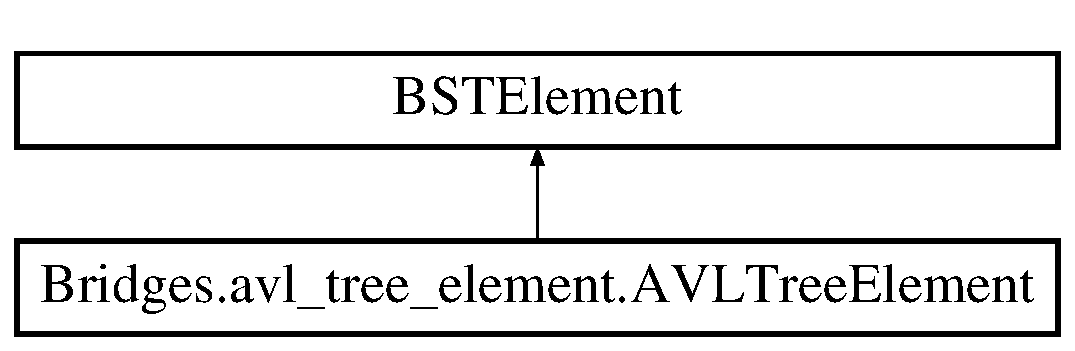
\includegraphics[height=2.000000cm]{class_bridges_1_1avl__tree__element_1_1_a_v_l_tree_element}
\end{center}
\end{figure}
\subsection*{Public Member Functions}
\begin{DoxyCompactItemize}
\item 
def \mbox{\hyperlink{class_bridges_1_1avl__tree__element_1_1_a_v_l_tree_element_af08d7ab277c031a48c00623fe09f7bca}{\+\_\+\+\_\+init\+\_\+\+\_\+}} (self, k=None, e=None)
\begin{DoxyCompactList}\small\item\em Construct an \mbox{\hyperlink{class_bridges_1_1avl__tree__element_1_1_a_v_l_tree_element}{A\+V\+L\+Tree\+Element}}. \end{DoxyCompactList}\item 
def \mbox{\hyperlink{class_bridges_1_1avl__tree__element_1_1_a_v_l_tree_element_a5981b0cdcaec83c3d8a013a7f7b83cb6}{get\+\_\+data\+\_\+structure\+\_\+type}} (self)
\begin{DoxyCompactList}\small\item\em This method gets the data structure type. \end{DoxyCompactList}\item 
def \mbox{\hyperlink{class_bridges_1_1avl__tree__element_1_1_a_v_l_tree_element_a3ce9e53b4a8267f966e50eee4e51854e}{get\+\_\+height}} (self)
\begin{DoxyCompactList}\small\item\em This method returns the height of the tree at this node. \end{DoxyCompactList}\item 
def \mbox{\hyperlink{class_bridges_1_1avl__tree__element_1_1_a_v_l_tree_element_a85482caa56d1556215de95f721b9892a}{set\+\_\+height}} (self, h)
\begin{DoxyCompactList}\small\item\em This method sets the height of the tree at this node. \end{DoxyCompactList}\item 
def \mbox{\hyperlink{class_bridges_1_1avl__tree__element_1_1_a_v_l_tree_element_ae3f1823a10539449a0a01c0a0449a46e}{get\+\_\+balance\+\_\+factor}} (self)
\begin{DoxyCompactList}\small\item\em This method returns the balance factor of the tree at this node. \end{DoxyCompactList}\item 
def \mbox{\hyperlink{class_bridges_1_1avl__tree__element_1_1_a_v_l_tree_element_a10507b26e6f83ded469db7fc280141d5}{set\+\_\+balance\+\_\+factor}} (self, bf)
\begin{DoxyCompactList}\small\item\em This method sets the balance factor of the tree at this node. \end{DoxyCompactList}\item 
def \mbox{\hyperlink{class_bridges_1_1avl__tree__element_1_1_a_v_l_tree_element_af534fdbf8ec5fe48aaf02ef9b8537b81}{get\+\_\+left}} (self)
\begin{DoxyCompactList}\small\item\em This method returns the left child of the tree node. \end{DoxyCompactList}\item 
def \mbox{\hyperlink{class_bridges_1_1avl__tree__element_1_1_a_v_l_tree_element_afc0e1b61a4e6e07192234d0975daaa9c}{get\+\_\+right}} (self)
\begin{DoxyCompactList}\small\item\em This method returns the right child of tree node. \end{DoxyCompactList}\end{DoxyCompactItemize}
\subsection*{Static Public Attributes}
\begin{DoxyCompactItemize}
\item 
\mbox{\hyperlink{class_bridges_1_1avl__tree__element_1_1_a_v_l_tree_element_ad4e11b61cca78051aea548c7fcb4e4fb}{height}} = int()
\item 
\mbox{\hyperlink{class_bridges_1_1avl__tree__element_1_1_a_v_l_tree_element_a9187ba8eeedf0e359f020b443275c356}{bal\+\_\+factor}} = int()
\end{DoxyCompactItemize}


\subsection{Detailed Description}
This class extends the B\+S\+T\+Element class by adding a height and balance factor fields that are useful in A\+VL trees. 

A\+VL tree elements include a \textquotesingle{}height\textquotesingle{} and a \textquotesingle{}bal\+Factor\textquotesingle{} value, representing the height and balance factor of the A\+VL tree at that node, respectively. This is useful in representing A\+VL trees.

A\+V\+L\+Tree elements contain a visualizer (Element\+Visualizer) object for setting visual attributes (color, shape, opacity, size), necessary for displaying them in a web browser.

A\+V\+L\+Tree elements also have a Link\+Visualizer object, that is used when they are linked to another element, appropriate for setting link attributes, for instance, between $\ast$ the current element and its left or right child

\begin{DoxyAuthor}{Author}
Kalpathi Subramanian, Mihai Mehedint
\end{DoxyAuthor}
\begin{DoxyDate}{Date}
6/22/16, 1/7/17, 5/17/17 
\end{DoxyDate}


\subsection{Constructor \& Destructor Documentation}
\mbox{\Hypertarget{class_bridges_1_1avl__tree__element_1_1_a_v_l_tree_element_af08d7ab277c031a48c00623fe09f7bca}\label{class_bridges_1_1avl__tree__element_1_1_a_v_l_tree_element_af08d7ab277c031a48c00623fe09f7bca}} 
\index{Bridges\+::avl\+\_\+tree\+\_\+element\+::\+A\+V\+L\+Tree\+Element@{Bridges\+::avl\+\_\+tree\+\_\+element\+::\+A\+V\+L\+Tree\+Element}!\+\_\+\+\_\+init\+\_\+\+\_\+@{\+\_\+\+\_\+init\+\_\+\+\_\+}}
\index{\+\_\+\+\_\+init\+\_\+\+\_\+@{\+\_\+\+\_\+init\+\_\+\+\_\+}!Bridges\+::avl\+\_\+tree\+\_\+element\+::\+A\+V\+L\+Tree\+Element@{Bridges\+::avl\+\_\+tree\+\_\+element\+::\+A\+V\+L\+Tree\+Element}}
\subsubsection{\texorpdfstring{\+\_\+\+\_\+init\+\_\+\+\_\+()}{\_\_init\_\_()}}
{\footnotesize\ttfamily def Bridges.\+avl\+\_\+tree\+\_\+element.\+A\+V\+L\+Tree\+Element.\+\_\+\+\_\+init\+\_\+\+\_\+ (\begin{DoxyParamCaption}\item[{}]{self,  }\item[{}]{k = {\ttfamily None},  }\item[{}]{e = {\ttfamily None} }\end{DoxyParamCaption})}



Construct an \mbox{\hyperlink{class_bridges_1_1avl__tree__element_1_1_a_v_l_tree_element}{A\+V\+L\+Tree\+Element}}. 


\begin{DoxyParams}{Parameters}
{\em k} & the search key \\
\hline
{\em e} & the appl specific object that Element is holding \\
\hline
\end{DoxyParams}


\subsection{Member Function Documentation}
\mbox{\Hypertarget{class_bridges_1_1avl__tree__element_1_1_a_v_l_tree_element_ae3f1823a10539449a0a01c0a0449a46e}\label{class_bridges_1_1avl__tree__element_1_1_a_v_l_tree_element_ae3f1823a10539449a0a01c0a0449a46e}} 
\index{Bridges\+::avl\+\_\+tree\+\_\+element\+::\+A\+V\+L\+Tree\+Element@{Bridges\+::avl\+\_\+tree\+\_\+element\+::\+A\+V\+L\+Tree\+Element}!get\+\_\+balance\+\_\+factor@{get\+\_\+balance\+\_\+factor}}
\index{get\+\_\+balance\+\_\+factor@{get\+\_\+balance\+\_\+factor}!Bridges\+::avl\+\_\+tree\+\_\+element\+::\+A\+V\+L\+Tree\+Element@{Bridges\+::avl\+\_\+tree\+\_\+element\+::\+A\+V\+L\+Tree\+Element}}
\subsubsection{\texorpdfstring{get\+\_\+balance\+\_\+factor()}{get\_balance\_factor()}}
{\footnotesize\ttfamily def Bridges.\+avl\+\_\+tree\+\_\+element.\+A\+V\+L\+Tree\+Element.\+get\+\_\+balance\+\_\+factor (\begin{DoxyParamCaption}\item[{}]{self }\end{DoxyParamCaption})}



This method returns the balance factor of the tree at this node. 

\begin{DoxyReturn}{Returns}
balance factor 
\end{DoxyReturn}
\mbox{\Hypertarget{class_bridges_1_1avl__tree__element_1_1_a_v_l_tree_element_a5981b0cdcaec83c3d8a013a7f7b83cb6}\label{class_bridges_1_1avl__tree__element_1_1_a_v_l_tree_element_a5981b0cdcaec83c3d8a013a7f7b83cb6}} 
\index{Bridges\+::avl\+\_\+tree\+\_\+element\+::\+A\+V\+L\+Tree\+Element@{Bridges\+::avl\+\_\+tree\+\_\+element\+::\+A\+V\+L\+Tree\+Element}!get\+\_\+data\+\_\+structure\+\_\+type@{get\+\_\+data\+\_\+structure\+\_\+type}}
\index{get\+\_\+data\+\_\+structure\+\_\+type@{get\+\_\+data\+\_\+structure\+\_\+type}!Bridges\+::avl\+\_\+tree\+\_\+element\+::\+A\+V\+L\+Tree\+Element@{Bridges\+::avl\+\_\+tree\+\_\+element\+::\+A\+V\+L\+Tree\+Element}}
\subsubsection{\texorpdfstring{get\+\_\+data\+\_\+structure\+\_\+type()}{get\_data\_structure\_type()}}
{\footnotesize\ttfamily def Bridges.\+avl\+\_\+tree\+\_\+element.\+A\+V\+L\+Tree\+Element.\+get\+\_\+data\+\_\+structure\+\_\+type (\begin{DoxyParamCaption}\item[{}]{self }\end{DoxyParamCaption})}



This method gets the data structure type. 

\begin{DoxyReturn}{Returns}
The date structure type as a string 
\end{DoxyReturn}
\mbox{\Hypertarget{class_bridges_1_1avl__tree__element_1_1_a_v_l_tree_element_a3ce9e53b4a8267f966e50eee4e51854e}\label{class_bridges_1_1avl__tree__element_1_1_a_v_l_tree_element_a3ce9e53b4a8267f966e50eee4e51854e}} 
\index{Bridges\+::avl\+\_\+tree\+\_\+element\+::\+A\+V\+L\+Tree\+Element@{Bridges\+::avl\+\_\+tree\+\_\+element\+::\+A\+V\+L\+Tree\+Element}!get\+\_\+height@{get\+\_\+height}}
\index{get\+\_\+height@{get\+\_\+height}!Bridges\+::avl\+\_\+tree\+\_\+element\+::\+A\+V\+L\+Tree\+Element@{Bridges\+::avl\+\_\+tree\+\_\+element\+::\+A\+V\+L\+Tree\+Element}}
\subsubsection{\texorpdfstring{get\+\_\+height()}{get\_height()}}
{\footnotesize\ttfamily def Bridges.\+avl\+\_\+tree\+\_\+element.\+A\+V\+L\+Tree\+Element.\+get\+\_\+height (\begin{DoxyParamCaption}\item[{}]{self }\end{DoxyParamCaption})}



This method returns the height of the tree at this node. 

\begin{DoxyReturn}{Returns}
height 
\end{DoxyReturn}
\mbox{\Hypertarget{class_bridges_1_1avl__tree__element_1_1_a_v_l_tree_element_af534fdbf8ec5fe48aaf02ef9b8537b81}\label{class_bridges_1_1avl__tree__element_1_1_a_v_l_tree_element_af534fdbf8ec5fe48aaf02ef9b8537b81}} 
\index{Bridges\+::avl\+\_\+tree\+\_\+element\+::\+A\+V\+L\+Tree\+Element@{Bridges\+::avl\+\_\+tree\+\_\+element\+::\+A\+V\+L\+Tree\+Element}!get\+\_\+left@{get\+\_\+left}}
\index{get\+\_\+left@{get\+\_\+left}!Bridges\+::avl\+\_\+tree\+\_\+element\+::\+A\+V\+L\+Tree\+Element@{Bridges\+::avl\+\_\+tree\+\_\+element\+::\+A\+V\+L\+Tree\+Element}}
\subsubsection{\texorpdfstring{get\+\_\+left()}{get\_left()}}
{\footnotesize\ttfamily def Bridges.\+avl\+\_\+tree\+\_\+element.\+A\+V\+L\+Tree\+Element.\+get\+\_\+left (\begin{DoxyParamCaption}\item[{}]{self }\end{DoxyParamCaption})}



This method returns the left child of the tree node. 

\begin{DoxyReturn}{Returns}
the left child of this node 
\end{DoxyReturn}
\mbox{\Hypertarget{class_bridges_1_1avl__tree__element_1_1_a_v_l_tree_element_afc0e1b61a4e6e07192234d0975daaa9c}\label{class_bridges_1_1avl__tree__element_1_1_a_v_l_tree_element_afc0e1b61a4e6e07192234d0975daaa9c}} 
\index{Bridges\+::avl\+\_\+tree\+\_\+element\+::\+A\+V\+L\+Tree\+Element@{Bridges\+::avl\+\_\+tree\+\_\+element\+::\+A\+V\+L\+Tree\+Element}!get\+\_\+right@{get\+\_\+right}}
\index{get\+\_\+right@{get\+\_\+right}!Bridges\+::avl\+\_\+tree\+\_\+element\+::\+A\+V\+L\+Tree\+Element@{Bridges\+::avl\+\_\+tree\+\_\+element\+::\+A\+V\+L\+Tree\+Element}}
\subsubsection{\texorpdfstring{get\+\_\+right()}{get\_right()}}
{\footnotesize\ttfamily def Bridges.\+avl\+\_\+tree\+\_\+element.\+A\+V\+L\+Tree\+Element.\+get\+\_\+right (\begin{DoxyParamCaption}\item[{}]{self }\end{DoxyParamCaption})}



This method returns the right child of tree node. 

\begin{DoxyReturn}{Returns}
the right child of this node 
\end{DoxyReturn}
\mbox{\Hypertarget{class_bridges_1_1avl__tree__element_1_1_a_v_l_tree_element_a10507b26e6f83ded469db7fc280141d5}\label{class_bridges_1_1avl__tree__element_1_1_a_v_l_tree_element_a10507b26e6f83ded469db7fc280141d5}} 
\index{Bridges\+::avl\+\_\+tree\+\_\+element\+::\+A\+V\+L\+Tree\+Element@{Bridges\+::avl\+\_\+tree\+\_\+element\+::\+A\+V\+L\+Tree\+Element}!set\+\_\+balance\+\_\+factor@{set\+\_\+balance\+\_\+factor}}
\index{set\+\_\+balance\+\_\+factor@{set\+\_\+balance\+\_\+factor}!Bridges\+::avl\+\_\+tree\+\_\+element\+::\+A\+V\+L\+Tree\+Element@{Bridges\+::avl\+\_\+tree\+\_\+element\+::\+A\+V\+L\+Tree\+Element}}
\subsubsection{\texorpdfstring{set\+\_\+balance\+\_\+factor()}{set\_balance\_factor()}}
{\footnotesize\ttfamily def Bridges.\+avl\+\_\+tree\+\_\+element.\+A\+V\+L\+Tree\+Element.\+set\+\_\+balance\+\_\+factor (\begin{DoxyParamCaption}\item[{}]{self,  }\item[{}]{bf }\end{DoxyParamCaption})}



This method sets the balance factor of the tree at this node. 


\begin{DoxyParams}{Parameters}
{\em balance} & factor bf \\
\hline
\end{DoxyParams}
\mbox{\Hypertarget{class_bridges_1_1avl__tree__element_1_1_a_v_l_tree_element_a85482caa56d1556215de95f721b9892a}\label{class_bridges_1_1avl__tree__element_1_1_a_v_l_tree_element_a85482caa56d1556215de95f721b9892a}} 
\index{Bridges\+::avl\+\_\+tree\+\_\+element\+::\+A\+V\+L\+Tree\+Element@{Bridges\+::avl\+\_\+tree\+\_\+element\+::\+A\+V\+L\+Tree\+Element}!set\+\_\+height@{set\+\_\+height}}
\index{set\+\_\+height@{set\+\_\+height}!Bridges\+::avl\+\_\+tree\+\_\+element\+::\+A\+V\+L\+Tree\+Element@{Bridges\+::avl\+\_\+tree\+\_\+element\+::\+A\+V\+L\+Tree\+Element}}
\subsubsection{\texorpdfstring{set\+\_\+height()}{set\_height()}}
{\footnotesize\ttfamily def Bridges.\+avl\+\_\+tree\+\_\+element.\+A\+V\+L\+Tree\+Element.\+set\+\_\+height (\begin{DoxyParamCaption}\item[{}]{self,  }\item[{}]{h }\end{DoxyParamCaption})}



This method sets the height of the tree at this node. 


\begin{DoxyParams}{Parameters}
{\em height} & h \\
\hline
\end{DoxyParams}


\subsection{Member Data Documentation}
\mbox{\Hypertarget{class_bridges_1_1avl__tree__element_1_1_a_v_l_tree_element_a9187ba8eeedf0e359f020b443275c356}\label{class_bridges_1_1avl__tree__element_1_1_a_v_l_tree_element_a9187ba8eeedf0e359f020b443275c356}} 
\index{Bridges\+::avl\+\_\+tree\+\_\+element\+::\+A\+V\+L\+Tree\+Element@{Bridges\+::avl\+\_\+tree\+\_\+element\+::\+A\+V\+L\+Tree\+Element}!bal\+\_\+factor@{bal\+\_\+factor}}
\index{bal\+\_\+factor@{bal\+\_\+factor}!Bridges\+::avl\+\_\+tree\+\_\+element\+::\+A\+V\+L\+Tree\+Element@{Bridges\+::avl\+\_\+tree\+\_\+element\+::\+A\+V\+L\+Tree\+Element}}
\subsubsection{\texorpdfstring{bal\+\_\+factor}{bal\_factor}}
{\footnotesize\ttfamily Bridges.\+avl\+\_\+tree\+\_\+element.\+A\+V\+L\+Tree\+Element.\+bal\+\_\+factor = int()\hspace{0.3cm}{\ttfamily [static]}}

\mbox{\Hypertarget{class_bridges_1_1avl__tree__element_1_1_a_v_l_tree_element_ad4e11b61cca78051aea548c7fcb4e4fb}\label{class_bridges_1_1avl__tree__element_1_1_a_v_l_tree_element_ad4e11b61cca78051aea548c7fcb4e4fb}} 
\index{Bridges\+::avl\+\_\+tree\+\_\+element\+::\+A\+V\+L\+Tree\+Element@{Bridges\+::avl\+\_\+tree\+\_\+element\+::\+A\+V\+L\+Tree\+Element}!height@{height}}
\index{height@{height}!Bridges\+::avl\+\_\+tree\+\_\+element\+::\+A\+V\+L\+Tree\+Element@{Bridges\+::avl\+\_\+tree\+\_\+element\+::\+A\+V\+L\+Tree\+Element}}
\subsubsection{\texorpdfstring{height}{height}}
{\footnotesize\ttfamily Bridges.\+avl\+\_\+tree\+\_\+element.\+A\+V\+L\+Tree\+Element.\+height = int()\hspace{0.3cm}{\ttfamily [static]}}



The documentation for this class was generated from the following file\+:\begin{DoxyCompactItemize}
\item 
/\+Users/kalpathi/gr/bridges/client/python/bridges18/\+Bridges/\mbox{\hyperlink{avl__tree__element_8py}{avl\+\_\+tree\+\_\+element.\+py}}\end{DoxyCompactItemize}

\hypertarget{class_bridges_1_1bin__tree__element_1_1_bin_tree_element}{}\section{Bridges.\+bin\+\_\+tree\+\_\+element.\+Bin\+Tree\+Element Class Reference}
\label{class_bridges_1_1bin__tree__element_1_1_bin_tree_element}\index{Bridges.\+bin\+\_\+tree\+\_\+element.\+Bin\+Tree\+Element@{Bridges.\+bin\+\_\+tree\+\_\+element.\+Bin\+Tree\+Element}}


This class is extended from the Tree\+Element class and can be used to create binary tree element objects.  


Inheritance diagram for Bridges.\+bin\+\_\+tree\+\_\+element.\+Bin\+Tree\+Element\+:\begin{figure}[H]
\begin{center}
\leavevmode
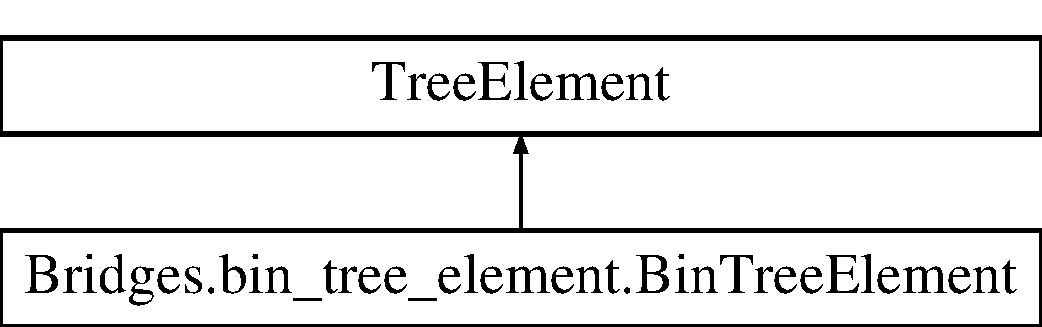
\includegraphics[height=2.000000cm]{class_bridges_1_1bin__tree__element_1_1_bin_tree_element}
\end{center}
\end{figure}
\subsection*{Public Member Functions}
\begin{DoxyCompactItemize}
\item 
def \hyperlink{class_bridges_1_1bin__tree__element_1_1_bin_tree_element_a55f0728b5c2d4ab4788c7af6a43d3799}{\+\_\+\+\_\+init\+\_\+\+\_\+}
\begin{DoxyCompactList}\small\item\em Constructs an empty Binary Tree Element. \end{DoxyCompactList}\item 
def \hyperlink{class_bridges_1_1bin__tree__element_1_1_bin_tree_element_af3618c59a2a576cb47b2f16433fcbac3}{get\+\_\+data\+\_\+structure\+\_\+type} (self)
\begin{DoxyCompactList}\small\item\em This method gets the data structure type. \end{DoxyCompactList}\item 
def \hyperlink{class_bridges_1_1bin__tree__element_1_1_bin_tree_element_a30ee0afc88fdbf55f7b645981dda73f2}{get\+\_\+left} (self)
\begin{DoxyCompactList}\small\item\em This method returns the left tree element pointer. \end{DoxyCompactList}\item 
def \hyperlink{class_bridges_1_1bin__tree__element_1_1_bin_tree_element_a4a86199c8090bcd7e603bccea2b5edff}{set\+\_\+left} (self, \hyperlink{class_bridges_1_1bin__tree__element_1_1_bin_tree_element_ae71553e3888615cdeb6fd8487045653c}{left})
\begin{DoxyCompactList}\small\item\em This method sets the left tree element pointer. \end{DoxyCompactList}\item 
def \hyperlink{class_bridges_1_1bin__tree__element_1_1_bin_tree_element_ae9e74ea73a3f5c27459344f1db42d9b6}{get\+\_\+right} (self)
\begin{DoxyCompactList}\small\item\em This method returns the right tree element pointer. \end{DoxyCompactList}\item 
def \hyperlink{class_bridges_1_1bin__tree__element_1_1_bin_tree_element_a171c46c251828f265ea8fb60b396f5b7}{set\+\_\+right} (self, \hyperlink{class_bridges_1_1bin__tree__element_1_1_bin_tree_element_acae42ce2d77e073ea539893c86103c17}{right})
\begin{DoxyCompactList}\small\item\em This method sets the right tree element pointer. \end{DoxyCompactList}\end{DoxyCompactItemize}
\subsection*{Static Public Attributes}
\begin{DoxyCompactItemize}
\item 
tuple \hyperlink{class_bridges_1_1bin__tree__element_1_1_bin_tree_element_ae71553e3888615cdeb6fd8487045653c}{left} = object()
\item 
tuple \hyperlink{class_bridges_1_1bin__tree__element_1_1_bin_tree_element_acae42ce2d77e073ea539893c86103c17}{right} = object()
\end{DoxyCompactItemize}


\subsection{Detailed Description}
This class is extended from the Tree\+Element class and can be used to create binary tree element objects. 

The Bin\+Tree element class is the building block for creating binary tree structures. It contains two children (viz., left, right).

\hyperlink{class_bridges_1_1bin__tree__element_1_1_bin_tree_element}{Bin\+Tree\+Element} contains a visualizer (Element\+Visualizer) object for setting visual attributes (color, shape, opacity, size), necessary for displaying them in a web browser.

Elements also have a Link\+Visualizer object, that is used when they are linked to another element, appropriate for setting link attributes, for instance, between the current element and its left or right child

\begin{DoxyAuthor}{Author}
Kalpathi Subramanian, Mihai Mehedint 
\end{DoxyAuthor}


\subsection{Constructor \& Destructor Documentation}
\hypertarget{class_bridges_1_1bin__tree__element_1_1_bin_tree_element_a55f0728b5c2d4ab4788c7af6a43d3799}{}\index{Bridges\+::bin\+\_\+tree\+\_\+element\+::\+Bin\+Tree\+Element@{Bridges\+::bin\+\_\+tree\+\_\+element\+::\+Bin\+Tree\+Element}!\+\_\+\+\_\+init\+\_\+\+\_\+@{\+\_\+\+\_\+init\+\_\+\+\_\+}}
\index{\+\_\+\+\_\+init\+\_\+\+\_\+@{\+\_\+\+\_\+init\+\_\+\+\_\+}!Bridges\+::bin\+\_\+tree\+\_\+element\+::\+Bin\+Tree\+Element@{Bridges\+::bin\+\_\+tree\+\_\+element\+::\+Bin\+Tree\+Element}}
\subsubsection[{\+\_\+\+\_\+init\+\_\+\+\_\+}]{\setlength{\rightskip}{0pt plus 5cm}def Bridges.\+bin\+\_\+tree\+\_\+element.\+Bin\+Tree\+Element.\+\_\+\+\_\+init\+\_\+\+\_\+ (
\begin{DoxyParamCaption}
\item[{}]{self, }
\item[{}]{label = {\ttfamily None}, }
\item[{}]{e = {\ttfamily None}, }
\item[{}]{left = {\ttfamily None}, }
\item[{}]{right = {\ttfamily None}}
\end{DoxyParamCaption}
)}\label{class_bridges_1_1bin__tree__element_1_1_bin_tree_element_a55f0728b5c2d4ab4788c7af6a43d3799}


Constructs an empty Binary Tree Element. 


\begin{DoxyParams}{Parameters}
{\em e} & the generic object that Tree\+Element will hold \\
\hline
{\em label} & the label of Tree\+Element that shows up on the bridges visualization \\
\hline
{\em left} & the Tree\+Element to be assigned to the left pointer of this Tree\+Element \\
\hline
{\em right} & the Tree\+Element to be assigned to the right pointer of this Tree\+Element \\
\hline
\end{DoxyParams}


\subsection{Member Function Documentation}
\hypertarget{class_bridges_1_1bin__tree__element_1_1_bin_tree_element_af3618c59a2a576cb47b2f16433fcbac3}{}\index{Bridges\+::bin\+\_\+tree\+\_\+element\+::\+Bin\+Tree\+Element@{Bridges\+::bin\+\_\+tree\+\_\+element\+::\+Bin\+Tree\+Element}!get\+\_\+data\+\_\+structure\+\_\+type@{get\+\_\+data\+\_\+structure\+\_\+type}}
\index{get\+\_\+data\+\_\+structure\+\_\+type@{get\+\_\+data\+\_\+structure\+\_\+type}!Bridges\+::bin\+\_\+tree\+\_\+element\+::\+Bin\+Tree\+Element@{Bridges\+::bin\+\_\+tree\+\_\+element\+::\+Bin\+Tree\+Element}}
\subsubsection[{get\+\_\+data\+\_\+structure\+\_\+type(self)}]{\setlength{\rightskip}{0pt plus 5cm}def Bridges.\+bin\+\_\+tree\+\_\+element.\+Bin\+Tree\+Element.\+get\+\_\+data\+\_\+structure\+\_\+type (
\begin{DoxyParamCaption}
\item[{}]{self}
\end{DoxyParamCaption}
)}\label{class_bridges_1_1bin__tree__element_1_1_bin_tree_element_af3618c59a2a576cb47b2f16433fcbac3}


This method gets the data structure type. 

\begin{DoxyReturn}{Returns}
The date structure type as a string 
\end{DoxyReturn}
\hypertarget{class_bridges_1_1bin__tree__element_1_1_bin_tree_element_a30ee0afc88fdbf55f7b645981dda73f2}{}\index{Bridges\+::bin\+\_\+tree\+\_\+element\+::\+Bin\+Tree\+Element@{Bridges\+::bin\+\_\+tree\+\_\+element\+::\+Bin\+Tree\+Element}!get\+\_\+left@{get\+\_\+left}}
\index{get\+\_\+left@{get\+\_\+left}!Bridges\+::bin\+\_\+tree\+\_\+element\+::\+Bin\+Tree\+Element@{Bridges\+::bin\+\_\+tree\+\_\+element\+::\+Bin\+Tree\+Element}}
\subsubsection[{get\+\_\+left(self)}]{\setlength{\rightskip}{0pt plus 5cm}def Bridges.\+bin\+\_\+tree\+\_\+element.\+Bin\+Tree\+Element.\+get\+\_\+left (
\begin{DoxyParamCaption}
\item[{}]{self}
\end{DoxyParamCaption}
)}\label{class_bridges_1_1bin__tree__element_1_1_bin_tree_element_a30ee0afc88fdbf55f7b645981dda73f2}


This method returns the left tree element pointer. 

\begin{DoxyReturn}{Returns}
the left child of this Tree\+Element 
\end{DoxyReturn}
\hypertarget{class_bridges_1_1bin__tree__element_1_1_bin_tree_element_ae9e74ea73a3f5c27459344f1db42d9b6}{}\index{Bridges\+::bin\+\_\+tree\+\_\+element\+::\+Bin\+Tree\+Element@{Bridges\+::bin\+\_\+tree\+\_\+element\+::\+Bin\+Tree\+Element}!get\+\_\+right@{get\+\_\+right}}
\index{get\+\_\+right@{get\+\_\+right}!Bridges\+::bin\+\_\+tree\+\_\+element\+::\+Bin\+Tree\+Element@{Bridges\+::bin\+\_\+tree\+\_\+element\+::\+Bin\+Tree\+Element}}
\subsubsection[{get\+\_\+right(self)}]{\setlength{\rightskip}{0pt plus 5cm}def Bridges.\+bin\+\_\+tree\+\_\+element.\+Bin\+Tree\+Element.\+get\+\_\+right (
\begin{DoxyParamCaption}
\item[{}]{self}
\end{DoxyParamCaption}
)}\label{class_bridges_1_1bin__tree__element_1_1_bin_tree_element_ae9e74ea73a3f5c27459344f1db42d9b6}


This method returns the right tree element pointer. 

\begin{DoxyReturn}{Returns}
the right child of this Tree\+Element 
\end{DoxyReturn}
\hypertarget{class_bridges_1_1bin__tree__element_1_1_bin_tree_element_a4a86199c8090bcd7e603bccea2b5edff}{}\index{Bridges\+::bin\+\_\+tree\+\_\+element\+::\+Bin\+Tree\+Element@{Bridges\+::bin\+\_\+tree\+\_\+element\+::\+Bin\+Tree\+Element}!set\+\_\+left@{set\+\_\+left}}
\index{set\+\_\+left@{set\+\_\+left}!Bridges\+::bin\+\_\+tree\+\_\+element\+::\+Bin\+Tree\+Element@{Bridges\+::bin\+\_\+tree\+\_\+element\+::\+Bin\+Tree\+Element}}
\subsubsection[{set\+\_\+left(self, left)}]{\setlength{\rightskip}{0pt plus 5cm}def Bridges.\+bin\+\_\+tree\+\_\+element.\+Bin\+Tree\+Element.\+set\+\_\+left (
\begin{DoxyParamCaption}
\item[{}]{self, }
\item[{}]{left}
\end{DoxyParamCaption}
)}\label{class_bridges_1_1bin__tree__element_1_1_bin_tree_element_a4a86199c8090bcd7e603bccea2b5edff}


This method sets the left tree element pointer. 


\begin{DoxyParams}{Parameters}
{\em left} & the Tree\+Element that should be assigned to the left child \\
\hline
\end{DoxyParams}
\hypertarget{class_bridges_1_1bin__tree__element_1_1_bin_tree_element_a171c46c251828f265ea8fb60b396f5b7}{}\index{Bridges\+::bin\+\_\+tree\+\_\+element\+::\+Bin\+Tree\+Element@{Bridges\+::bin\+\_\+tree\+\_\+element\+::\+Bin\+Tree\+Element}!set\+\_\+right@{set\+\_\+right}}
\index{set\+\_\+right@{set\+\_\+right}!Bridges\+::bin\+\_\+tree\+\_\+element\+::\+Bin\+Tree\+Element@{Bridges\+::bin\+\_\+tree\+\_\+element\+::\+Bin\+Tree\+Element}}
\subsubsection[{set\+\_\+right(self, right)}]{\setlength{\rightskip}{0pt plus 5cm}def Bridges.\+bin\+\_\+tree\+\_\+element.\+Bin\+Tree\+Element.\+set\+\_\+right (
\begin{DoxyParamCaption}
\item[{}]{self, }
\item[{}]{right}
\end{DoxyParamCaption}
)}\label{class_bridges_1_1bin__tree__element_1_1_bin_tree_element_a171c46c251828f265ea8fb60b396f5b7}


This method sets the right tree element pointer. 


\begin{DoxyParams}{Parameters}
{\em right} & the Tree\+Element that should be assigned to the right child \\
\hline
\end{DoxyParams}


\subsection{Member Data Documentation}
\hypertarget{class_bridges_1_1bin__tree__element_1_1_bin_tree_element_ae71553e3888615cdeb6fd8487045653c}{}\index{Bridges\+::bin\+\_\+tree\+\_\+element\+::\+Bin\+Tree\+Element@{Bridges\+::bin\+\_\+tree\+\_\+element\+::\+Bin\+Tree\+Element}!left@{left}}
\index{left@{left}!Bridges\+::bin\+\_\+tree\+\_\+element\+::\+Bin\+Tree\+Element@{Bridges\+::bin\+\_\+tree\+\_\+element\+::\+Bin\+Tree\+Element}}
\subsubsection[{left}]{\setlength{\rightskip}{0pt plus 5cm}tuple Bridges.\+bin\+\_\+tree\+\_\+element.\+Bin\+Tree\+Element.\+left = object()\hspace{0.3cm}{\ttfamily [static]}}\label{class_bridges_1_1bin__tree__element_1_1_bin_tree_element_ae71553e3888615cdeb6fd8487045653c}
\hypertarget{class_bridges_1_1bin__tree__element_1_1_bin_tree_element_acae42ce2d77e073ea539893c86103c17}{}\index{Bridges\+::bin\+\_\+tree\+\_\+element\+::\+Bin\+Tree\+Element@{Bridges\+::bin\+\_\+tree\+\_\+element\+::\+Bin\+Tree\+Element}!right@{right}}
\index{right@{right}!Bridges\+::bin\+\_\+tree\+\_\+element\+::\+Bin\+Tree\+Element@{Bridges\+::bin\+\_\+tree\+\_\+element\+::\+Bin\+Tree\+Element}}
\subsubsection[{right}]{\setlength{\rightskip}{0pt plus 5cm}tuple Bridges.\+bin\+\_\+tree\+\_\+element.\+Bin\+Tree\+Element.\+right = object()\hspace{0.3cm}{\ttfamily [static]}}\label{class_bridges_1_1bin__tree__element_1_1_bin_tree_element_acae42ce2d77e073ea539893c86103c17}


The documentation for this class was generated from the following file\+:\begin{DoxyCompactItemize}
\item 
/\+Users/kalpathi/gr/bridges/client/python/\+Bridges/\hyperlink{bin__tree__element_8py}{bin\+\_\+tree\+\_\+element.\+py}\end{DoxyCompactItemize}

\hypertarget{class_bridges_1_1bridges_1_1_bridges}{}\section{Bridges.\+bridges.\+Bridges Class Reference}
\label{class_bridges_1_1bridges_1_1_bridges}\index{Bridges.\+bridges.\+Bridges@{Bridges.\+bridges.\+Bridges}}


The bridges class is the main class that provides interfaces to datasets, maintains user and assignment information, and connects to the bridges server.  


\subsection*{Public Member Functions}
\begin{DoxyCompactItemize}
\item 
def \mbox{\hyperlink{class_bridges_1_1bridges_1_1_bridges_ad3a26dd5ee8dea00adbc5345e4f313d6}{\+\_\+\+\_\+init\+\_\+\+\_\+}} (self, \mbox{\hyperlink{class_bridges_1_1bridges_1_1_bridges_a66e278ddefd9a2c94c01eb0fc9bbc568}{assignment}}, \mbox{\hyperlink{class_bridges_1_1bridges_1_1_bridges_a09593511340ae03bed2abbf9dd12f48f}{username}}, appl\+\_\+id)
\begin{DoxyCompactList}\small\item\em Initialize bridges (Constructor) \end{DoxyCompactList}\item 
def \mbox{\hyperlink{class_bridges_1_1bridges_1_1_bridges_adab1ccb3816211bc81054f8fb537833f}{set\+\_\+data\+\_\+structure}} (self, ds)
\begin{DoxyCompactList}\small\item\em This method sets the handle to the current data structure; this can be an array, the head of a linked list, root of a tree structure, a graph Arrays of upto 3 dimensions are suppported. \end{DoxyCompactList}\item 
def \mbox{\hyperlink{class_bridges_1_1bridges_1_1_bridges_a945f547bc7feb7e129811f8874a3af6b}{set\+\_\+visualize\+\_\+\+J\+S\+ON}} (self, flag)
\item 
def \mbox{\hyperlink{class_bridges_1_1bridges_1_1_bridges_ad25ec4119ef21f031c6240a9d6d996c6}{visualize}} (self)
\begin{DoxyCompactList}\small\item\em This method generates the representation of the current data structure (J\+S\+ON) and sends that to the bridges server for generating a visualization. \end{DoxyCompactList}\item 
def \mbox{\hyperlink{class_bridges_1_1bridges_1_1_bridges_a7a8e13b7b0908c9d0bce26c5ad41c32e}{set\+\_\+assignment}} (self, \mbox{\hyperlink{class_bridges_1_1bridges_1_1_bridges_a66e278ddefd9a2c94c01eb0fc9bbc568}{assignment}})
\begin{DoxyCompactList}\small\item\em set the assignment id \end{DoxyCompactList}\item 
def \mbox{\hyperlink{class_bridges_1_1bridges_1_1_bridges_ac65a74c86b8b2e456f43cf731daae085}{get\+\_\+assignment}} (self)
\begin{DoxyCompactList}\small\item\em Get the assignment id. \end{DoxyCompactList}\item 
def \mbox{\hyperlink{class_bridges_1_1bridges_1_1_bridges_a1732ccf3904c3de48f697feff32b95a5}{set\+\_\+title}} (self, \mbox{\hyperlink{class_bridges_1_1bridges_1_1_bridges_a5427643899fb1ddfc7d4d834779409bd}{title}})
\item 
def \mbox{\hyperlink{class_bridges_1_1bridges_1_1_bridges_aa9af47e59998f5d9659c4d49295c6ece}{set\+\_\+description}} (self, \mbox{\hyperlink{class_bridges_1_1bridges_1_1_bridges_adf7716495f589eef1236200869f22679}{description}})
\item 
def \mbox{\hyperlink{class_bridges_1_1bridges_1_1_bridges_ae051d3b37125d0806f15a0990df5885c}{set\+\_\+map\+\_\+overlay}} (self, flag)
\item 
def \mbox{\hyperlink{class_bridges_1_1bridges_1_1_bridges_a6e70886184cb4735961507d9e84eb8fe}{set\+\_\+coord\+\_\+system\+\_\+type}} (self, coord)
\item 
def \mbox{\hyperlink{class_bridges_1_1bridges_1_1_bridges_a88c1a0909a08065f31c5d0868e9d1900}{get\+\_\+color\+\_\+grid\+\_\+from\+\_\+assignment}}
\end{DoxyCompactItemize}
\subsection*{Public Attributes}
\begin{DoxyCompactItemize}
\item 
\mbox{\hyperlink{class_bridges_1_1bridges_1_1_bridges_a0ec63234eea5146e87f0572972a7f41d}{key}}
\item 
\mbox{\hyperlink{class_bridges_1_1bridges_1_1_bridges_a178b38dd8e06bcd4e57527301454ba12}{connector}}
\item 
\mbox{\hyperlink{class_bridges_1_1bridges_1_1_bridges_afe26b5521aae689055377e6f2e6a7212}{username}}
\item 
\mbox{\hyperlink{class_bridges_1_1bridges_1_1_bridges_ae5c5349721fdc457fcae13ed370ba1d8}{coord\+\_\+system\+\_\+type}}
\item 
\mbox{\hyperlink{class_bridges_1_1bridges_1_1_bridges_a0c3729b756ec663959e99210d986638e}{vis\+\_\+type}}
\item 
\mbox{\hyperlink{class_bridges_1_1bridges_1_1_bridges_a93088231d5f240848046e8065330aa4f}{json\+\_\+flag}}
\item 
\mbox{\hyperlink{class_bridges_1_1bridges_1_1_bridges_a925840aac84da0d17db238e5628d5f1a}{map\+\_\+overlay}}
\end{DoxyCompactItemize}
\subsection*{Static Public Attributes}
\begin{DoxyCompactItemize}
\item 
string \mbox{\hyperlink{class_bridges_1_1bridges_1_1_bridges_aec289f4a18867c2fef080a4faa092e8e}{vis\+\_\+type}} = \char`\"{}\char`\"{}
\item 
\mbox{\hyperlink{class_bridges_1_1bridges_1_1_bridges_abfb616560e034d466cd624132d3a96a3}{ds\+\_\+handle}} = None
\item 
\mbox{\hyperlink{class_bridges_1_1bridges_1_1_bridges_a5427643899fb1ddfc7d4d834779409bd}{title}} = str()
\item 
\mbox{\hyperlink{class_bridges_1_1bridges_1_1_bridges_adf7716495f589eef1236200869f22679}{description}} = str()
\item 
string \mbox{\hyperlink{class_bridges_1_1bridges_1_1_bridges_a82068879504b788bb70470fd04bc3c55}{coord\+\_\+system\+\_\+type}} = \char`\"{}cartesian\char`\"{}
\item 
bool \mbox{\hyperlink{class_bridges_1_1bridges_1_1_bridges_aa4c998e01d5c0f16f9a278c01c02af7d}{map\+\_\+overlay}} = False
\item 
string \mbox{\hyperlink{class_bridges_1_1bridges_1_1_bridges_a09593511340ae03bed2abbf9dd12f48f}{username}} = \char`\"{}\char`\"{}
\item 
\mbox{\hyperlink{class_bridges_1_1bridges_1_1_bridges_a66e278ddefd9a2c94c01eb0fc9bbc568}{assignment}} = int()
\item 
\mbox{\hyperlink{class_bridges_1_1bridges_1_1_bridges_aab0a68541bf63b6c234c50514f1cbe80}{assignment\+\_\+part}} = int()
\item 
bool \mbox{\hyperlink{class_bridges_1_1bridges_1_1_bridges_a2a47934ce69f65d9d6df6d294db3968b}{json\+\_\+flag}} = False
\item 
dictionary \mbox{\hyperlink{class_bridges_1_1bridges_1_1_bridges_a0e1ec4382d41e2f268dbf37ac583c803}{projection\+\_\+options}} = \{\char`\"{}cartesian\char`\"{}, \char`\"{}albersusa\char`\"{}, \char`\"{}equirectangular\char`\"{}\}
\item 
string \mbox{\hyperlink{class_bridges_1_1bridges_1_1_bridges_afb82742483cfcad189739b6f772b8a12}{Q\+U\+O\+TE}} = \char`\"{}\textbackslash{}\char`\"{}\char`\"{}
\item 
string \mbox{\hyperlink{class_bridges_1_1bridges_1_1_bridges_a009b6e8d4a7c23a014ed8e5089eb7357}{C\+O\+M\+MA}} = \char`\"{},\char`\"{}
\item 
string \mbox{\hyperlink{class_bridges_1_1bridges_1_1_bridges_abfa62a66fca4dae2fe727a590a284f6b}{C\+O\+L\+ON}} = \char`\"{}\+:\char`\"{}
\item 
string \mbox{\hyperlink{class_bridges_1_1bridges_1_1_bridges_a2553c7dc637582bfd38998ee5c2a7f2b}{O\+P\+E\+N\+\_\+\+C\+U\+R\+LY}} = \char`\"{}\{\char`\"{}
\item 
string \mbox{\hyperlink{class_bridges_1_1bridges_1_1_bridges_ac4c7b26ef4e060229b1449ab73500cfb}{C\+L\+O\+S\+E\+\_\+\+C\+U\+R\+LY}} = \char`\"{}\}\char`\"{}
\item 
string \mbox{\hyperlink{class_bridges_1_1bridges_1_1_bridges_a1cd80e923a43de668fe44b606264b290}{O\+P\+E\+N\+\_\+\+P\+A\+R\+EN}} = \char`\"{}(\char`\"{}
\item 
string \mbox{\hyperlink{class_bridges_1_1bridges_1_1_bridges_a0b250d3bfad480552ff46884310ac6d1}{C\+L\+O\+S\+E\+\_\+\+P\+A\+R\+EN}} = \char`\"{})\char`\"{}
\item 
string \mbox{\hyperlink{class_bridges_1_1bridges_1_1_bridges_ae766e7f43cc4c93ff14abff689aa6612}{O\+P\+E\+N\+\_\+\+B\+OX}} = \char`\"{}\mbox{[}\char`\"{}
\item 
string \mbox{\hyperlink{class_bridges_1_1bridges_1_1_bridges_ae389d89d8512b2c481da3c165cac4c33}{C\+L\+O\+S\+E\+\_\+\+B\+OX}} = \char`\"{}\mbox{]}\char`\"{}
\end{DoxyCompactItemize}


\subsection{Detailed Description}
The bridges class is the main class that provides interfaces to datasets, maintains user and assignment information, and connects to the bridges server. 

The bridges class is responsible for initializing the bridges system, specifying parameters (user id, assignment id, title, description, data structure type, etc) for the student assignment, generating the data structure representation and transmission to the bridges server. In addition, it provides interfaces to a number of real-\/world datasets, that makes it easy to access the data for use algorithms/data structure assignments. ~\newline


{\bfseries Datasets.} The datasets that are currently supported through the B\+R\+I\+D\+G\+ES A\+PI include U\+S\+GS Earthquake Data, I\+M\+DB Actor/\+Movie Data (2 versions), Gutenberg Book Collection Meta Data, a Video Game Dataset and Shakespeare Dataset. More information is found in the respective methods (below) and at 

\href{http://bridgesuncc.github.io/datasets.html}{\tt http\+://bridgesuncc.\+github.\+io/datasets.\+html} 

A typical bridges program includes creating the bridges object, followed by creation of the data structure by the user, assigning visual attributes to elements of the data structure, followed by specification of teh data structure type and the call to visualize the data structure (bridges\+::set\+Data\+Structure() and \mbox{\hyperlink{class_bridges_1_1bridges_1_1_bridges_ad25ec4119ef21f031c6240a9d6d996c6}{visualize()}} methods).

\begin{DoxyAuthor}{Author}
Sean Gallagher, Kalpathi Subramanaian, Mihai Mehedint, David Burlinson. 
\end{DoxyAuthor}


\subsection{Constructor \& Destructor Documentation}
\mbox{\Hypertarget{class_bridges_1_1bridges_1_1_bridges_ad3a26dd5ee8dea00adbc5345e4f313d6}\label{class_bridges_1_1bridges_1_1_bridges_ad3a26dd5ee8dea00adbc5345e4f313d6}} 
\index{Bridges\+::bridges\+::\+Bridges@{Bridges\+::bridges\+::\+Bridges}!\+\_\+\+\_\+init\+\_\+\+\_\+@{\+\_\+\+\_\+init\+\_\+\+\_\+}}
\index{\+\_\+\+\_\+init\+\_\+\+\_\+@{\+\_\+\+\_\+init\+\_\+\+\_\+}!Bridges\+::bridges\+::\+Bridges@{Bridges\+::bridges\+::\+Bridges}}
\subsubsection{\texorpdfstring{\+\_\+\+\_\+init\+\_\+\+\_\+()}{\_\_init\_\_()}}
{\footnotesize\ttfamily def Bridges.\+bridges.\+Bridges.\+\_\+\+\_\+init\+\_\+\+\_\+ (\begin{DoxyParamCaption}\item[{}]{self,  }\item[{}]{assignment,  }\item[{}]{username,  }\item[{}]{appl\+\_\+id }\end{DoxyParamCaption})}



Initialize bridges (Constructor) 


\begin{DoxyParams}{Parameters}
{\em assignment} & this is the assignmen id (integer) \\
\hline
{\em appl\+\_\+id} & this is the appl authentication key(from the bridges account) \\
\hline
{\em username} & this is the username (from the bridges account) \\
\hline
\end{DoxyParams}


\subsection{Member Function Documentation}
\mbox{\Hypertarget{class_bridges_1_1bridges_1_1_bridges_ac65a74c86b8b2e456f43cf731daae085}\label{class_bridges_1_1bridges_1_1_bridges_ac65a74c86b8b2e456f43cf731daae085}} 
\index{Bridges\+::bridges\+::\+Bridges@{Bridges\+::bridges\+::\+Bridges}!get\+\_\+assignment@{get\+\_\+assignment}}
\index{get\+\_\+assignment@{get\+\_\+assignment}!Bridges\+::bridges\+::\+Bridges@{Bridges\+::bridges\+::\+Bridges}}
\subsubsection{\texorpdfstring{get\+\_\+assignment()}{get\_assignment()}}
{\footnotesize\ttfamily def Bridges.\+bridges.\+Bridges.\+get\+\_\+assignment (\begin{DoxyParamCaption}\item[{}]{self }\end{DoxyParamCaption})}



Get the assignment id. 

\begin{DoxyReturn}{Returns}
assignment as a string 
\end{DoxyReturn}
\mbox{\Hypertarget{class_bridges_1_1bridges_1_1_bridges_a88c1a0909a08065f31c5d0868e9d1900}\label{class_bridges_1_1bridges_1_1_bridges_a88c1a0909a08065f31c5d0868e9d1900}} 
\index{Bridges\+::bridges\+::\+Bridges@{Bridges\+::bridges\+::\+Bridges}!get\+\_\+color\+\_\+grid\+\_\+from\+\_\+assignment@{get\+\_\+color\+\_\+grid\+\_\+from\+\_\+assignment}}
\index{get\+\_\+color\+\_\+grid\+\_\+from\+\_\+assignment@{get\+\_\+color\+\_\+grid\+\_\+from\+\_\+assignment}!Bridges\+::bridges\+::\+Bridges@{Bridges\+::bridges\+::\+Bridges}}
\subsubsection{\texorpdfstring{get\+\_\+color\+\_\+grid\+\_\+from\+\_\+assignment()}{get\_color\_grid\_from\_assignment()}}
{\footnotesize\ttfamily def Bridges.\+bridges.\+Bridges.\+get\+\_\+color\+\_\+grid\+\_\+from\+\_\+assignment (\begin{DoxyParamCaption}\item[{}]{self,  }\item[{}]{user }\end{DoxyParamCaption})}

\mbox{\Hypertarget{class_bridges_1_1bridges_1_1_bridges_a7a8e13b7b0908c9d0bce26c5ad41c32e}\label{class_bridges_1_1bridges_1_1_bridges_a7a8e13b7b0908c9d0bce26c5ad41c32e}} 
\index{Bridges\+::bridges\+::\+Bridges@{Bridges\+::bridges\+::\+Bridges}!set\+\_\+assignment@{set\+\_\+assignment}}
\index{set\+\_\+assignment@{set\+\_\+assignment}!Bridges\+::bridges\+::\+Bridges@{Bridges\+::bridges\+::\+Bridges}}
\subsubsection{\texorpdfstring{set\+\_\+assignment()}{set\_assignment()}}
{\footnotesize\ttfamily def Bridges.\+bridges.\+Bridges.\+set\+\_\+assignment (\begin{DoxyParamCaption}\item[{}]{self,  }\item[{}]{assignment }\end{DoxyParamCaption})}



set the assignment id 


\begin{DoxyParams}{Parameters}
{\em assignment} & number \\
\hline
\end{DoxyParams}
\mbox{\Hypertarget{class_bridges_1_1bridges_1_1_bridges_a6e70886184cb4735961507d9e84eb8fe}\label{class_bridges_1_1bridges_1_1_bridges_a6e70886184cb4735961507d9e84eb8fe}} 
\index{Bridges\+::bridges\+::\+Bridges@{Bridges\+::bridges\+::\+Bridges}!set\+\_\+coord\+\_\+system\+\_\+type@{set\+\_\+coord\+\_\+system\+\_\+type}}
\index{set\+\_\+coord\+\_\+system\+\_\+type@{set\+\_\+coord\+\_\+system\+\_\+type}!Bridges\+::bridges\+::\+Bridges@{Bridges\+::bridges\+::\+Bridges}}
\subsubsection{\texorpdfstring{set\+\_\+coord\+\_\+system\+\_\+type()}{set\_coord\_system\_type()}}
{\footnotesize\ttfamily def Bridges.\+bridges.\+Bridges.\+set\+\_\+coord\+\_\+system\+\_\+type (\begin{DoxyParamCaption}\item[{}]{self,  }\item[{}]{coord }\end{DoxyParamCaption})}

\mbox{\Hypertarget{class_bridges_1_1bridges_1_1_bridges_adab1ccb3816211bc81054f8fb537833f}\label{class_bridges_1_1bridges_1_1_bridges_adab1ccb3816211bc81054f8fb537833f}} 
\index{Bridges\+::bridges\+::\+Bridges@{Bridges\+::bridges\+::\+Bridges}!set\+\_\+data\+\_\+structure@{set\+\_\+data\+\_\+structure}}
\index{set\+\_\+data\+\_\+structure@{set\+\_\+data\+\_\+structure}!Bridges\+::bridges\+::\+Bridges@{Bridges\+::bridges\+::\+Bridges}}
\subsubsection{\texorpdfstring{set\+\_\+data\+\_\+structure()}{set\_data\_structure()}}
{\footnotesize\ttfamily def Bridges.\+bridges.\+Bridges.\+set\+\_\+data\+\_\+structure (\begin{DoxyParamCaption}\item[{}]{self,  }\item[{}]{ds }\end{DoxyParamCaption})}



This method sets the handle to the current data structure; this can be an array, the head of a linked list, root of a tree structure, a graph Arrays of upto 3 dimensions are suppported. 

It can be any of the data structures supported by B\+R\+I\+D\+G\+ES. Polymorphism and type casting is used to determine the actual data structure and extract its representtion.


\begin{DoxyParams}{Parameters}
{\em ds} & The data structure to set (any of the subclasses of Data\+Struct) \\
\hline
\end{DoxyParams}
\mbox{\Hypertarget{class_bridges_1_1bridges_1_1_bridges_aa9af47e59998f5d9659c4d49295c6ece}\label{class_bridges_1_1bridges_1_1_bridges_aa9af47e59998f5d9659c4d49295c6ece}} 
\index{Bridges\+::bridges\+::\+Bridges@{Bridges\+::bridges\+::\+Bridges}!set\+\_\+description@{set\+\_\+description}}
\index{set\+\_\+description@{set\+\_\+description}!Bridges\+::bridges\+::\+Bridges@{Bridges\+::bridges\+::\+Bridges}}
\subsubsection{\texorpdfstring{set\+\_\+description()}{set\_description()}}
{\footnotesize\ttfamily def Bridges.\+bridges.\+Bridges.\+set\+\_\+description (\begin{DoxyParamCaption}\item[{}]{self,  }\item[{}]{description }\end{DoxyParamCaption})}


\begin{DoxyParams}{Parameters}
{\em description} & description to annotate the visualization; \\
\hline
\end{DoxyParams}
\mbox{\Hypertarget{class_bridges_1_1bridges_1_1_bridges_ae051d3b37125d0806f15a0990df5885c}\label{class_bridges_1_1bridges_1_1_bridges_ae051d3b37125d0806f15a0990df5885c}} 
\index{Bridges\+::bridges\+::\+Bridges@{Bridges\+::bridges\+::\+Bridges}!set\+\_\+map\+\_\+overlay@{set\+\_\+map\+\_\+overlay}}
\index{set\+\_\+map\+\_\+overlay@{set\+\_\+map\+\_\+overlay}!Bridges\+::bridges\+::\+Bridges@{Bridges\+::bridges\+::\+Bridges}}
\subsubsection{\texorpdfstring{set\+\_\+map\+\_\+overlay()}{set\_map\_overlay()}}
{\footnotesize\ttfamily def Bridges.\+bridges.\+Bridges.\+set\+\_\+map\+\_\+overlay (\begin{DoxyParamCaption}\item[{}]{self,  }\item[{}]{flag }\end{DoxyParamCaption})}

\mbox{\Hypertarget{class_bridges_1_1bridges_1_1_bridges_a1732ccf3904c3de48f697feff32b95a5}\label{class_bridges_1_1bridges_1_1_bridges_a1732ccf3904c3de48f697feff32b95a5}} 
\index{Bridges\+::bridges\+::\+Bridges@{Bridges\+::bridges\+::\+Bridges}!set\+\_\+title@{set\+\_\+title}}
\index{set\+\_\+title@{set\+\_\+title}!Bridges\+::bridges\+::\+Bridges@{Bridges\+::bridges\+::\+Bridges}}
\subsubsection{\texorpdfstring{set\+\_\+title()}{set\_title()}}
{\footnotesize\ttfamily def Bridges.\+bridges.\+Bridges.\+set\+\_\+title (\begin{DoxyParamCaption}\item[{}]{self,  }\item[{}]{title }\end{DoxyParamCaption})}


\begin{DoxyParams}{Parameters}
{\em title} & title used in the visualization; \\
\hline
\end{DoxyParams}
\mbox{\Hypertarget{class_bridges_1_1bridges_1_1_bridges_a945f547bc7feb7e129811f8874a3af6b}\label{class_bridges_1_1bridges_1_1_bridges_a945f547bc7feb7e129811f8874a3af6b}} 
\index{Bridges\+::bridges\+::\+Bridges@{Bridges\+::bridges\+::\+Bridges}!set\+\_\+visualize\+\_\+\+J\+S\+ON@{set\+\_\+visualize\+\_\+\+J\+S\+ON}}
\index{set\+\_\+visualize\+\_\+\+J\+S\+ON@{set\+\_\+visualize\+\_\+\+J\+S\+ON}!Bridges\+::bridges\+::\+Bridges@{Bridges\+::bridges\+::\+Bridges}}
\subsubsection{\texorpdfstring{set\+\_\+visualize\+\_\+\+J\+S\+O\+N()}{set\_visualize\_JSON()}}
{\footnotesize\ttfamily def Bridges.\+bridges.\+Bridges.\+set\+\_\+visualize\+\_\+\+J\+S\+ON (\begin{DoxyParamCaption}\item[{}]{self,  }\item[{}]{flag }\end{DoxyParamCaption})}

\mbox{\Hypertarget{class_bridges_1_1bridges_1_1_bridges_ad25ec4119ef21f031c6240a9d6d996c6}\label{class_bridges_1_1bridges_1_1_bridges_ad25ec4119ef21f031c6240a9d6d996c6}} 
\index{Bridges\+::bridges\+::\+Bridges@{Bridges\+::bridges\+::\+Bridges}!visualize@{visualize}}
\index{visualize@{visualize}!Bridges\+::bridges\+::\+Bridges@{Bridges\+::bridges\+::\+Bridges}}
\subsubsection{\texorpdfstring{visualize()}{visualize()}}
{\footnotesize\ttfamily def Bridges.\+bridges.\+Bridges.\+visualize (\begin{DoxyParamCaption}\item[{}]{self }\end{DoxyParamCaption})}



This method generates the representation of the current data structure (J\+S\+ON) and sends that to the bridges server for generating a visualization. 



\subsection{Member Data Documentation}
\mbox{\Hypertarget{class_bridges_1_1bridges_1_1_bridges_a66e278ddefd9a2c94c01eb0fc9bbc568}\label{class_bridges_1_1bridges_1_1_bridges_a66e278ddefd9a2c94c01eb0fc9bbc568}} 
\index{Bridges\+::bridges\+::\+Bridges@{Bridges\+::bridges\+::\+Bridges}!assignment@{assignment}}
\index{assignment@{assignment}!Bridges\+::bridges\+::\+Bridges@{Bridges\+::bridges\+::\+Bridges}}
\subsubsection{\texorpdfstring{assignment}{assignment}}
{\footnotesize\ttfamily Bridges.\+bridges.\+Bridges.\+assignment = int()\hspace{0.3cm}{\ttfamily [static]}}

\mbox{\Hypertarget{class_bridges_1_1bridges_1_1_bridges_aab0a68541bf63b6c234c50514f1cbe80}\label{class_bridges_1_1bridges_1_1_bridges_aab0a68541bf63b6c234c50514f1cbe80}} 
\index{Bridges\+::bridges\+::\+Bridges@{Bridges\+::bridges\+::\+Bridges}!assignment\+\_\+part@{assignment\+\_\+part}}
\index{assignment\+\_\+part@{assignment\+\_\+part}!Bridges\+::bridges\+::\+Bridges@{Bridges\+::bridges\+::\+Bridges}}
\subsubsection{\texorpdfstring{assignment\+\_\+part}{assignment\_part}}
{\footnotesize\ttfamily Bridges.\+bridges.\+Bridges.\+assignment\+\_\+part = int()\hspace{0.3cm}{\ttfamily [static]}}

\mbox{\Hypertarget{class_bridges_1_1bridges_1_1_bridges_ae389d89d8512b2c481da3c165cac4c33}\label{class_bridges_1_1bridges_1_1_bridges_ae389d89d8512b2c481da3c165cac4c33}} 
\index{Bridges\+::bridges\+::\+Bridges@{Bridges\+::bridges\+::\+Bridges}!C\+L\+O\+S\+E\+\_\+\+B\+OX@{C\+L\+O\+S\+E\+\_\+\+B\+OX}}
\index{C\+L\+O\+S\+E\+\_\+\+B\+OX@{C\+L\+O\+S\+E\+\_\+\+B\+OX}!Bridges\+::bridges\+::\+Bridges@{Bridges\+::bridges\+::\+Bridges}}
\subsubsection{\texorpdfstring{C\+L\+O\+S\+E\+\_\+\+B\+OX}{CLOSE\_BOX}}
{\footnotesize\ttfamily string Bridges.\+bridges.\+Bridges.\+C\+L\+O\+S\+E\+\_\+\+B\+OX = \char`\"{}\mbox{]}\char`\"{}\hspace{0.3cm}{\ttfamily [static]}}

\mbox{\Hypertarget{class_bridges_1_1bridges_1_1_bridges_ac4c7b26ef4e060229b1449ab73500cfb}\label{class_bridges_1_1bridges_1_1_bridges_ac4c7b26ef4e060229b1449ab73500cfb}} 
\index{Bridges\+::bridges\+::\+Bridges@{Bridges\+::bridges\+::\+Bridges}!C\+L\+O\+S\+E\+\_\+\+C\+U\+R\+LY@{C\+L\+O\+S\+E\+\_\+\+C\+U\+R\+LY}}
\index{C\+L\+O\+S\+E\+\_\+\+C\+U\+R\+LY@{C\+L\+O\+S\+E\+\_\+\+C\+U\+R\+LY}!Bridges\+::bridges\+::\+Bridges@{Bridges\+::bridges\+::\+Bridges}}
\subsubsection{\texorpdfstring{C\+L\+O\+S\+E\+\_\+\+C\+U\+R\+LY}{CLOSE\_CURLY}}
{\footnotesize\ttfamily string Bridges.\+bridges.\+Bridges.\+C\+L\+O\+S\+E\+\_\+\+C\+U\+R\+LY = \char`\"{}\}\char`\"{}\hspace{0.3cm}{\ttfamily [static]}}

\mbox{\Hypertarget{class_bridges_1_1bridges_1_1_bridges_a0b250d3bfad480552ff46884310ac6d1}\label{class_bridges_1_1bridges_1_1_bridges_a0b250d3bfad480552ff46884310ac6d1}} 
\index{Bridges\+::bridges\+::\+Bridges@{Bridges\+::bridges\+::\+Bridges}!C\+L\+O\+S\+E\+\_\+\+P\+A\+R\+EN@{C\+L\+O\+S\+E\+\_\+\+P\+A\+R\+EN}}
\index{C\+L\+O\+S\+E\+\_\+\+P\+A\+R\+EN@{C\+L\+O\+S\+E\+\_\+\+P\+A\+R\+EN}!Bridges\+::bridges\+::\+Bridges@{Bridges\+::bridges\+::\+Bridges}}
\subsubsection{\texorpdfstring{C\+L\+O\+S\+E\+\_\+\+P\+A\+R\+EN}{CLOSE\_PAREN}}
{\footnotesize\ttfamily string Bridges.\+bridges.\+Bridges.\+C\+L\+O\+S\+E\+\_\+\+P\+A\+R\+EN = \char`\"{})\char`\"{}\hspace{0.3cm}{\ttfamily [static]}}

\mbox{\Hypertarget{class_bridges_1_1bridges_1_1_bridges_abfa62a66fca4dae2fe727a590a284f6b}\label{class_bridges_1_1bridges_1_1_bridges_abfa62a66fca4dae2fe727a590a284f6b}} 
\index{Bridges\+::bridges\+::\+Bridges@{Bridges\+::bridges\+::\+Bridges}!C\+O\+L\+ON@{C\+O\+L\+ON}}
\index{C\+O\+L\+ON@{C\+O\+L\+ON}!Bridges\+::bridges\+::\+Bridges@{Bridges\+::bridges\+::\+Bridges}}
\subsubsection{\texorpdfstring{C\+O\+L\+ON}{COLON}}
{\footnotesize\ttfamily string Bridges.\+bridges.\+Bridges.\+C\+O\+L\+ON = \char`\"{}\+:\char`\"{}\hspace{0.3cm}{\ttfamily [static]}}

\mbox{\Hypertarget{class_bridges_1_1bridges_1_1_bridges_a009b6e8d4a7c23a014ed8e5089eb7357}\label{class_bridges_1_1bridges_1_1_bridges_a009b6e8d4a7c23a014ed8e5089eb7357}} 
\index{Bridges\+::bridges\+::\+Bridges@{Bridges\+::bridges\+::\+Bridges}!C\+O\+M\+MA@{C\+O\+M\+MA}}
\index{C\+O\+M\+MA@{C\+O\+M\+MA}!Bridges\+::bridges\+::\+Bridges@{Bridges\+::bridges\+::\+Bridges}}
\subsubsection{\texorpdfstring{C\+O\+M\+MA}{COMMA}}
{\footnotesize\ttfamily string Bridges.\+bridges.\+Bridges.\+C\+O\+M\+MA = \char`\"{},\char`\"{}\hspace{0.3cm}{\ttfamily [static]}}

\mbox{\Hypertarget{class_bridges_1_1bridges_1_1_bridges_a178b38dd8e06bcd4e57527301454ba12}\label{class_bridges_1_1bridges_1_1_bridges_a178b38dd8e06bcd4e57527301454ba12}} 
\index{Bridges\+::bridges\+::\+Bridges@{Bridges\+::bridges\+::\+Bridges}!connector@{connector}}
\index{connector@{connector}!Bridges\+::bridges\+::\+Bridges@{Bridges\+::bridges\+::\+Bridges}}
\subsubsection{\texorpdfstring{connector}{connector}}
{\footnotesize\ttfamily Bridges.\+bridges.\+Bridges.\+connector}

\mbox{\Hypertarget{class_bridges_1_1bridges_1_1_bridges_a82068879504b788bb70470fd04bc3c55}\label{class_bridges_1_1bridges_1_1_bridges_a82068879504b788bb70470fd04bc3c55}} 
\index{Bridges\+::bridges\+::\+Bridges@{Bridges\+::bridges\+::\+Bridges}!coord\+\_\+system\+\_\+type@{coord\+\_\+system\+\_\+type}}
\index{coord\+\_\+system\+\_\+type@{coord\+\_\+system\+\_\+type}!Bridges\+::bridges\+::\+Bridges@{Bridges\+::bridges\+::\+Bridges}}
\subsubsection{\texorpdfstring{coord\+\_\+system\+\_\+type}{coord\_system\_type}\hspace{0.1cm}{\footnotesize\ttfamily [1/2]}}
{\footnotesize\ttfamily string Bridges.\+bridges.\+Bridges.\+coord\+\_\+system\+\_\+type = \char`\"{}cartesian\char`\"{}\hspace{0.3cm}{\ttfamily [static]}}

\mbox{\Hypertarget{class_bridges_1_1bridges_1_1_bridges_ae5c5349721fdc457fcae13ed370ba1d8}\label{class_bridges_1_1bridges_1_1_bridges_ae5c5349721fdc457fcae13ed370ba1d8}} 
\index{Bridges\+::bridges\+::\+Bridges@{Bridges\+::bridges\+::\+Bridges}!coord\+\_\+system\+\_\+type@{coord\+\_\+system\+\_\+type}}
\index{coord\+\_\+system\+\_\+type@{coord\+\_\+system\+\_\+type}!Bridges\+::bridges\+::\+Bridges@{Bridges\+::bridges\+::\+Bridges}}
\subsubsection{\texorpdfstring{coord\+\_\+system\+\_\+type}{coord\_system\_type}\hspace{0.1cm}{\footnotesize\ttfamily [2/2]}}
{\footnotesize\ttfamily Bridges.\+bridges.\+Bridges.\+coord\+\_\+system\+\_\+type}

\mbox{\Hypertarget{class_bridges_1_1bridges_1_1_bridges_adf7716495f589eef1236200869f22679}\label{class_bridges_1_1bridges_1_1_bridges_adf7716495f589eef1236200869f22679}} 
\index{Bridges\+::bridges\+::\+Bridges@{Bridges\+::bridges\+::\+Bridges}!description@{description}}
\index{description@{description}!Bridges\+::bridges\+::\+Bridges@{Bridges\+::bridges\+::\+Bridges}}
\subsubsection{\texorpdfstring{description}{description}}
{\footnotesize\ttfamily Bridges.\+bridges.\+Bridges.\+description = str()\hspace{0.3cm}{\ttfamily [static]}}

\mbox{\Hypertarget{class_bridges_1_1bridges_1_1_bridges_abfb616560e034d466cd624132d3a96a3}\label{class_bridges_1_1bridges_1_1_bridges_abfb616560e034d466cd624132d3a96a3}} 
\index{Bridges\+::bridges\+::\+Bridges@{Bridges\+::bridges\+::\+Bridges}!ds\+\_\+handle@{ds\+\_\+handle}}
\index{ds\+\_\+handle@{ds\+\_\+handle}!Bridges\+::bridges\+::\+Bridges@{Bridges\+::bridges\+::\+Bridges}}
\subsubsection{\texorpdfstring{ds\+\_\+handle}{ds\_handle}}
{\footnotesize\ttfamily Bridges.\+bridges.\+Bridges.\+ds\+\_\+handle = None\hspace{0.3cm}{\ttfamily [static]}}

\mbox{\Hypertarget{class_bridges_1_1bridges_1_1_bridges_a2a47934ce69f65d9d6df6d294db3968b}\label{class_bridges_1_1bridges_1_1_bridges_a2a47934ce69f65d9d6df6d294db3968b}} 
\index{Bridges\+::bridges\+::\+Bridges@{Bridges\+::bridges\+::\+Bridges}!json\+\_\+flag@{json\+\_\+flag}}
\index{json\+\_\+flag@{json\+\_\+flag}!Bridges\+::bridges\+::\+Bridges@{Bridges\+::bridges\+::\+Bridges}}
\subsubsection{\texorpdfstring{json\+\_\+flag}{json\_flag}\hspace{0.1cm}{\footnotesize\ttfamily [1/2]}}
{\footnotesize\ttfamily bool Bridges.\+bridges.\+Bridges.\+json\+\_\+flag = False\hspace{0.3cm}{\ttfamily [static]}}

\mbox{\Hypertarget{class_bridges_1_1bridges_1_1_bridges_a93088231d5f240848046e8065330aa4f}\label{class_bridges_1_1bridges_1_1_bridges_a93088231d5f240848046e8065330aa4f}} 
\index{Bridges\+::bridges\+::\+Bridges@{Bridges\+::bridges\+::\+Bridges}!json\+\_\+flag@{json\+\_\+flag}}
\index{json\+\_\+flag@{json\+\_\+flag}!Bridges\+::bridges\+::\+Bridges@{Bridges\+::bridges\+::\+Bridges}}
\subsubsection{\texorpdfstring{json\+\_\+flag}{json\_flag}\hspace{0.1cm}{\footnotesize\ttfamily [2/2]}}
{\footnotesize\ttfamily Bridges.\+bridges.\+Bridges.\+json\+\_\+flag}

\mbox{\Hypertarget{class_bridges_1_1bridges_1_1_bridges_a0ec63234eea5146e87f0572972a7f41d}\label{class_bridges_1_1bridges_1_1_bridges_a0ec63234eea5146e87f0572972a7f41d}} 
\index{Bridges\+::bridges\+::\+Bridges@{Bridges\+::bridges\+::\+Bridges}!key@{key}}
\index{key@{key}!Bridges\+::bridges\+::\+Bridges@{Bridges\+::bridges\+::\+Bridges}}
\subsubsection{\texorpdfstring{key}{key}}
{\footnotesize\ttfamily Bridges.\+bridges.\+Bridges.\+key}

\mbox{\Hypertarget{class_bridges_1_1bridges_1_1_bridges_aa4c998e01d5c0f16f9a278c01c02af7d}\label{class_bridges_1_1bridges_1_1_bridges_aa4c998e01d5c0f16f9a278c01c02af7d}} 
\index{Bridges\+::bridges\+::\+Bridges@{Bridges\+::bridges\+::\+Bridges}!map\+\_\+overlay@{map\+\_\+overlay}}
\index{map\+\_\+overlay@{map\+\_\+overlay}!Bridges\+::bridges\+::\+Bridges@{Bridges\+::bridges\+::\+Bridges}}
\subsubsection{\texorpdfstring{map\+\_\+overlay}{map\_overlay}\hspace{0.1cm}{\footnotesize\ttfamily [1/2]}}
{\footnotesize\ttfamily bool Bridges.\+bridges.\+Bridges.\+map\+\_\+overlay = False\hspace{0.3cm}{\ttfamily [static]}}

\mbox{\Hypertarget{class_bridges_1_1bridges_1_1_bridges_a925840aac84da0d17db238e5628d5f1a}\label{class_bridges_1_1bridges_1_1_bridges_a925840aac84da0d17db238e5628d5f1a}} 
\index{Bridges\+::bridges\+::\+Bridges@{Bridges\+::bridges\+::\+Bridges}!map\+\_\+overlay@{map\+\_\+overlay}}
\index{map\+\_\+overlay@{map\+\_\+overlay}!Bridges\+::bridges\+::\+Bridges@{Bridges\+::bridges\+::\+Bridges}}
\subsubsection{\texorpdfstring{map\+\_\+overlay}{map\_overlay}\hspace{0.1cm}{\footnotesize\ttfamily [2/2]}}
{\footnotesize\ttfamily Bridges.\+bridges.\+Bridges.\+map\+\_\+overlay}

\mbox{\Hypertarget{class_bridges_1_1bridges_1_1_bridges_ae766e7f43cc4c93ff14abff689aa6612}\label{class_bridges_1_1bridges_1_1_bridges_ae766e7f43cc4c93ff14abff689aa6612}} 
\index{Bridges\+::bridges\+::\+Bridges@{Bridges\+::bridges\+::\+Bridges}!O\+P\+E\+N\+\_\+\+B\+OX@{O\+P\+E\+N\+\_\+\+B\+OX}}
\index{O\+P\+E\+N\+\_\+\+B\+OX@{O\+P\+E\+N\+\_\+\+B\+OX}!Bridges\+::bridges\+::\+Bridges@{Bridges\+::bridges\+::\+Bridges}}
\subsubsection{\texorpdfstring{O\+P\+E\+N\+\_\+\+B\+OX}{OPEN\_BOX}}
{\footnotesize\ttfamily string Bridges.\+bridges.\+Bridges.\+O\+P\+E\+N\+\_\+\+B\+OX = \char`\"{}\mbox{[}\char`\"{}\hspace{0.3cm}{\ttfamily [static]}}

\mbox{\Hypertarget{class_bridges_1_1bridges_1_1_bridges_a2553c7dc637582bfd38998ee5c2a7f2b}\label{class_bridges_1_1bridges_1_1_bridges_a2553c7dc637582bfd38998ee5c2a7f2b}} 
\index{Bridges\+::bridges\+::\+Bridges@{Bridges\+::bridges\+::\+Bridges}!O\+P\+E\+N\+\_\+\+C\+U\+R\+LY@{O\+P\+E\+N\+\_\+\+C\+U\+R\+LY}}
\index{O\+P\+E\+N\+\_\+\+C\+U\+R\+LY@{O\+P\+E\+N\+\_\+\+C\+U\+R\+LY}!Bridges\+::bridges\+::\+Bridges@{Bridges\+::bridges\+::\+Bridges}}
\subsubsection{\texorpdfstring{O\+P\+E\+N\+\_\+\+C\+U\+R\+LY}{OPEN\_CURLY}}
{\footnotesize\ttfamily string Bridges.\+bridges.\+Bridges.\+O\+P\+E\+N\+\_\+\+C\+U\+R\+LY = \char`\"{}\{\char`\"{}\hspace{0.3cm}{\ttfamily [static]}}

\mbox{\Hypertarget{class_bridges_1_1bridges_1_1_bridges_a1cd80e923a43de668fe44b606264b290}\label{class_bridges_1_1bridges_1_1_bridges_a1cd80e923a43de668fe44b606264b290}} 
\index{Bridges\+::bridges\+::\+Bridges@{Bridges\+::bridges\+::\+Bridges}!O\+P\+E\+N\+\_\+\+P\+A\+R\+EN@{O\+P\+E\+N\+\_\+\+P\+A\+R\+EN}}
\index{O\+P\+E\+N\+\_\+\+P\+A\+R\+EN@{O\+P\+E\+N\+\_\+\+P\+A\+R\+EN}!Bridges\+::bridges\+::\+Bridges@{Bridges\+::bridges\+::\+Bridges}}
\subsubsection{\texorpdfstring{O\+P\+E\+N\+\_\+\+P\+A\+R\+EN}{OPEN\_PAREN}}
{\footnotesize\ttfamily string Bridges.\+bridges.\+Bridges.\+O\+P\+E\+N\+\_\+\+P\+A\+R\+EN = \char`\"{}(\char`\"{}\hspace{0.3cm}{\ttfamily [static]}}

\mbox{\Hypertarget{class_bridges_1_1bridges_1_1_bridges_a0e1ec4382d41e2f268dbf37ac583c803}\label{class_bridges_1_1bridges_1_1_bridges_a0e1ec4382d41e2f268dbf37ac583c803}} 
\index{Bridges\+::bridges\+::\+Bridges@{Bridges\+::bridges\+::\+Bridges}!projection\+\_\+options@{projection\+\_\+options}}
\index{projection\+\_\+options@{projection\+\_\+options}!Bridges\+::bridges\+::\+Bridges@{Bridges\+::bridges\+::\+Bridges}}
\subsubsection{\texorpdfstring{projection\+\_\+options}{projection\_options}}
{\footnotesize\ttfamily dictionary Bridges.\+bridges.\+Bridges.\+projection\+\_\+options = \{\char`\"{}cartesian\char`\"{}, \char`\"{}albersusa\char`\"{}, \char`\"{}equirectangular\char`\"{}\}\hspace{0.3cm}{\ttfamily [static]}}

\mbox{\Hypertarget{class_bridges_1_1bridges_1_1_bridges_afb82742483cfcad189739b6f772b8a12}\label{class_bridges_1_1bridges_1_1_bridges_afb82742483cfcad189739b6f772b8a12}} 
\index{Bridges\+::bridges\+::\+Bridges@{Bridges\+::bridges\+::\+Bridges}!Q\+U\+O\+TE@{Q\+U\+O\+TE}}
\index{Q\+U\+O\+TE@{Q\+U\+O\+TE}!Bridges\+::bridges\+::\+Bridges@{Bridges\+::bridges\+::\+Bridges}}
\subsubsection{\texorpdfstring{Q\+U\+O\+TE}{QUOTE}}
{\footnotesize\ttfamily string Bridges.\+bridges.\+Bridges.\+Q\+U\+O\+TE = \char`\"{}\textbackslash{}\char`\"{}\char`\"{}\hspace{0.3cm}{\ttfamily [static]}}

\mbox{\Hypertarget{class_bridges_1_1bridges_1_1_bridges_a5427643899fb1ddfc7d4d834779409bd}\label{class_bridges_1_1bridges_1_1_bridges_a5427643899fb1ddfc7d4d834779409bd}} 
\index{Bridges\+::bridges\+::\+Bridges@{Bridges\+::bridges\+::\+Bridges}!title@{title}}
\index{title@{title}!Bridges\+::bridges\+::\+Bridges@{Bridges\+::bridges\+::\+Bridges}}
\subsubsection{\texorpdfstring{title}{title}}
{\footnotesize\ttfamily Bridges.\+bridges.\+Bridges.\+title = str()\hspace{0.3cm}{\ttfamily [static]}}

\mbox{\Hypertarget{class_bridges_1_1bridges_1_1_bridges_a09593511340ae03bed2abbf9dd12f48f}\label{class_bridges_1_1bridges_1_1_bridges_a09593511340ae03bed2abbf9dd12f48f}} 
\index{Bridges\+::bridges\+::\+Bridges@{Bridges\+::bridges\+::\+Bridges}!username@{username}}
\index{username@{username}!Bridges\+::bridges\+::\+Bridges@{Bridges\+::bridges\+::\+Bridges}}
\subsubsection{\texorpdfstring{username}{username}\hspace{0.1cm}{\footnotesize\ttfamily [1/2]}}
{\footnotesize\ttfamily string Bridges.\+bridges.\+Bridges.\+username = \char`\"{}\char`\"{}\hspace{0.3cm}{\ttfamily [static]}}

\mbox{\Hypertarget{class_bridges_1_1bridges_1_1_bridges_afe26b5521aae689055377e6f2e6a7212}\label{class_bridges_1_1bridges_1_1_bridges_afe26b5521aae689055377e6f2e6a7212}} 
\index{Bridges\+::bridges\+::\+Bridges@{Bridges\+::bridges\+::\+Bridges}!username@{username}}
\index{username@{username}!Bridges\+::bridges\+::\+Bridges@{Bridges\+::bridges\+::\+Bridges}}
\subsubsection{\texorpdfstring{username}{username}\hspace{0.1cm}{\footnotesize\ttfamily [2/2]}}
{\footnotesize\ttfamily Bridges.\+bridges.\+Bridges.\+username}

\mbox{\Hypertarget{class_bridges_1_1bridges_1_1_bridges_aec289f4a18867c2fef080a4faa092e8e}\label{class_bridges_1_1bridges_1_1_bridges_aec289f4a18867c2fef080a4faa092e8e}} 
\index{Bridges\+::bridges\+::\+Bridges@{Bridges\+::bridges\+::\+Bridges}!vis\+\_\+type@{vis\+\_\+type}}
\index{vis\+\_\+type@{vis\+\_\+type}!Bridges\+::bridges\+::\+Bridges@{Bridges\+::bridges\+::\+Bridges}}
\subsubsection{\texorpdfstring{vis\+\_\+type}{vis\_type}\hspace{0.1cm}{\footnotesize\ttfamily [1/2]}}
{\footnotesize\ttfamily string Bridges.\+bridges.\+Bridges.\+vis\+\_\+type = \char`\"{}\char`\"{}\hspace{0.3cm}{\ttfamily [static]}}

\mbox{\Hypertarget{class_bridges_1_1bridges_1_1_bridges_a0c3729b756ec663959e99210d986638e}\label{class_bridges_1_1bridges_1_1_bridges_a0c3729b756ec663959e99210d986638e}} 
\index{Bridges\+::bridges\+::\+Bridges@{Bridges\+::bridges\+::\+Bridges}!vis\+\_\+type@{vis\+\_\+type}}
\index{vis\+\_\+type@{vis\+\_\+type}!Bridges\+::bridges\+::\+Bridges@{Bridges\+::bridges\+::\+Bridges}}
\subsubsection{\texorpdfstring{vis\+\_\+type}{vis\_type}\hspace{0.1cm}{\footnotesize\ttfamily [2/2]}}
{\footnotesize\ttfamily Bridges.\+bridges.\+Bridges.\+vis\+\_\+type}



The documentation for this class was generated from the following file\+:\begin{DoxyCompactItemize}
\item 
/\+Users/kalpathi/gr/bridges/client/python/bridges18/\+Bridges/\mbox{\hyperlink{bridges_8py}{bridges.\+py}}\end{DoxyCompactItemize}

\hypertarget{class_bridges_1_1bst__element_1_1_b_s_t_element}{}\section{Bridges.\+bst\+\_\+element.\+B\+S\+T\+Element Class Reference}
\label{class_bridges_1_1bst__element_1_1_b_s_t_element}\index{Bridges.\+bst\+\_\+element.\+B\+S\+T\+Element@{Bridges.\+bst\+\_\+element.\+B\+S\+T\+Element}}


The \mbox{\hyperlink{class_bridges_1_1bst__element_1_1_b_s_t_element}{B\+S\+T\+Element}} class is the building block for creating binary search trees.  


Inheritance diagram for Bridges.\+bst\+\_\+element.\+B\+S\+T\+Element\+:\begin{figure}[H]
\begin{center}
\leavevmode
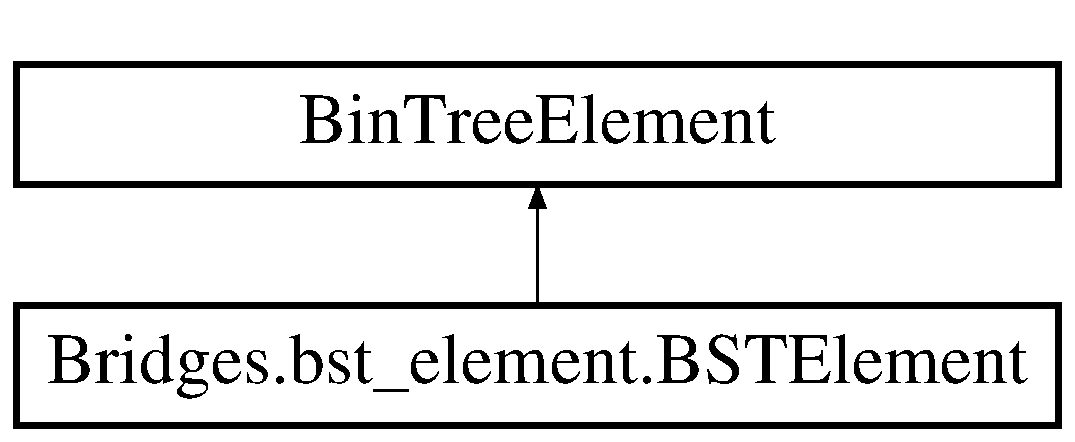
\includegraphics[height=2.000000cm]{class_bridges_1_1bst__element_1_1_b_s_t_element}
\end{center}
\end{figure}
\subsection*{Public Member Functions}
\begin{DoxyCompactItemize}
\item 
def \mbox{\hyperlink{class_bridges_1_1bst__element_1_1_b_s_t_element_a2d8abd4eca8f2643df2159aa12a920bf}{\+\_\+\+\_\+init\+\_\+\+\_\+}} (self, \mbox{\hyperlink{class_bridges_1_1bst__element_1_1_b_s_t_element_a1b04a3676ac84d889491f8a496aedb91}{key}}=None, e=None, left=None, right=None, label=None)
\begin{DoxyCompactList}\small\item\em Construct an empty \mbox{\hyperlink{class_bridges_1_1bst__element_1_1_b_s_t_element}{B\+S\+T\+Element}} with no key assigned and left and right pointers set to null. \end{DoxyCompactList}\item 
def \mbox{\hyperlink{class_bridges_1_1bst__element_1_1_b_s_t_element_a2ae53418d5efb075d9e63c675f4cdcdb}{get\+\_\+data\+\_\+structure\+\_\+type}} (self)
\begin{DoxyCompactList}\small\item\em This method gets the data structure type. \end{DoxyCompactList}\item 
def \mbox{\hyperlink{class_bridges_1_1bst__element_1_1_b_s_t_element_ac0ec75f813b838cf0f817ca6e4814766}{get\+\_\+key}} (self)
\begin{DoxyCompactList}\small\item\em Return the key of the \mbox{\hyperlink{class_bridges_1_1bst__element_1_1_b_s_t_element}{B\+S\+T\+Element}}. \end{DoxyCompactList}\item 
def \mbox{\hyperlink{class_bridges_1_1bst__element_1_1_b_s_t_element_ad72900f1e40534cbfe8b88d37e391750}{set\+\_\+key}} (self, \mbox{\hyperlink{class_bridges_1_1bst__element_1_1_b_s_t_element_a1b04a3676ac84d889491f8a496aedb91}{key}})
\begin{DoxyCompactList}\small\item\em Set the key of the \mbox{\hyperlink{class_bridges_1_1bst__element_1_1_b_s_t_element}{B\+S\+T\+Element}} to key. \end{DoxyCompactList}\item 
def \mbox{\hyperlink{class_bridges_1_1bst__element_1_1_b_s_t_element_a7f12207f3859f60be107468000cc2375}{get\+\_\+left}} (self)
\begin{DoxyCompactList}\small\item\em Return the left child of the \mbox{\hyperlink{class_bridges_1_1bst__element_1_1_b_s_t_element}{B\+S\+T\+Element}}. \end{DoxyCompactList}\item 
def \mbox{\hyperlink{class_bridges_1_1bst__element_1_1_b_s_t_element_a96c3a91946f244720054c2d480a05955}{get\+\_\+right}} (self)
\begin{DoxyCompactList}\small\item\em Return the right child of the \mbox{\hyperlink{class_bridges_1_1bst__element_1_1_b_s_t_element}{B\+S\+T\+Element}}. \end{DoxyCompactList}\end{DoxyCompactItemize}
\subsection*{Static Public Attributes}
\begin{DoxyCompactItemize}
\item 
\mbox{\hyperlink{class_bridges_1_1bst__element_1_1_b_s_t_element_a1b04a3676ac84d889491f8a496aedb91}{key}} = object()
\end{DoxyCompactItemize}


\subsection{Detailed Description}
The \mbox{\hyperlink{class_bridges_1_1bst__element_1_1_b_s_t_element}{B\+S\+T\+Element}} class is the building block for creating binary search trees. 

The \mbox{\hyperlink{class_bridges_1_1bst__element_1_1_b_s_t_element}{B\+S\+T\+Element}} class is the building block for creating binary search tree structures. It contains two children (viz., left, right), and a search key, to be used in search operations .

\mbox{\hyperlink{class_bridges_1_1bst__element_1_1_b_s_t_element}{B\+S\+T\+Element}} contains a visualizer (Element\+Visualizer) object for setting visual attributes (color, shape, opacity, size), necessary for displaying them in a web browser.

B\+ST Elements also have a Link\+Visualizer object, that is used when they are linked to another element, appropriate for setting link attributes, for instance, between the current element and its left or right child

\begin{DoxyAuthor}{Author}
Kalpathi Subramanian, Mihai Mehedint
\end{DoxyAuthor}
\begin{DoxyDate}{Date}
6/22/16, 1/7/17, 5/17/17
\end{DoxyDate}
This class extends the Bin\+Tree\+Element class by adding a \textquotesingle{}key\textquotesingle{} value for use in a binary search tree implementations. 

\subsection{Constructor \& Destructor Documentation}
\mbox{\Hypertarget{class_bridges_1_1bst__element_1_1_b_s_t_element_a2d8abd4eca8f2643df2159aa12a920bf}\label{class_bridges_1_1bst__element_1_1_b_s_t_element_a2d8abd4eca8f2643df2159aa12a920bf}} 
\index{Bridges\+::bst\+\_\+element\+::\+B\+S\+T\+Element@{Bridges\+::bst\+\_\+element\+::\+B\+S\+T\+Element}!\+\_\+\+\_\+init\+\_\+\+\_\+@{\+\_\+\+\_\+init\+\_\+\+\_\+}}
\index{\+\_\+\+\_\+init\+\_\+\+\_\+@{\+\_\+\+\_\+init\+\_\+\+\_\+}!Bridges\+::bst\+\_\+element\+::\+B\+S\+T\+Element@{Bridges\+::bst\+\_\+element\+::\+B\+S\+T\+Element}}
\subsubsection{\texorpdfstring{\+\_\+\+\_\+init\+\_\+\+\_\+()}{\_\_init\_\_()}}
{\footnotesize\ttfamily def Bridges.\+bst\+\_\+element.\+B\+S\+T\+Element.\+\_\+\+\_\+init\+\_\+\+\_\+ (\begin{DoxyParamCaption}\item[{}]{self,  }\item[{}]{key = {\ttfamily None},  }\item[{}]{e = {\ttfamily None},  }\item[{}]{left = {\ttfamily None},  }\item[{}]{right = {\ttfamily None},  }\item[{}]{label = {\ttfamily None} }\end{DoxyParamCaption})}



Construct an empty \mbox{\hyperlink{class_bridges_1_1bst__element_1_1_b_s_t_element}{B\+S\+T\+Element}} with no key assigned and left and right pointers set to null. 


\begin{DoxyParams}{Parameters}
{\em key} & the key to be used in a binary search tree implementation \\
\hline
{\em e} & the object this \mbox{\hyperlink{class_bridges_1_1bst__element_1_1_b_s_t_element}{B\+S\+T\+Element}} is holding \\
\hline
{\em left} & the \mbox{\hyperlink{class_bridges_1_1bst__element_1_1_b_s_t_element}{B\+S\+T\+Element}} that should be assigned to the left pointer \\
\hline
{\em right} & the \mbox{\hyperlink{class_bridges_1_1bst__element_1_1_b_s_t_element}{B\+S\+T\+Element}} that should be assigned to the right pointer \\
\hline
\end{DoxyParams}


\subsection{Member Function Documentation}
\mbox{\Hypertarget{class_bridges_1_1bst__element_1_1_b_s_t_element_a2ae53418d5efb075d9e63c675f4cdcdb}\label{class_bridges_1_1bst__element_1_1_b_s_t_element_a2ae53418d5efb075d9e63c675f4cdcdb}} 
\index{Bridges\+::bst\+\_\+element\+::\+B\+S\+T\+Element@{Bridges\+::bst\+\_\+element\+::\+B\+S\+T\+Element}!get\+\_\+data\+\_\+structure\+\_\+type@{get\+\_\+data\+\_\+structure\+\_\+type}}
\index{get\+\_\+data\+\_\+structure\+\_\+type@{get\+\_\+data\+\_\+structure\+\_\+type}!Bridges\+::bst\+\_\+element\+::\+B\+S\+T\+Element@{Bridges\+::bst\+\_\+element\+::\+B\+S\+T\+Element}}
\subsubsection{\texorpdfstring{get\+\_\+data\+\_\+structure\+\_\+type()}{get\_data\_structure\_type()}}
{\footnotesize\ttfamily def Bridges.\+bst\+\_\+element.\+B\+S\+T\+Element.\+get\+\_\+data\+\_\+structure\+\_\+type (\begin{DoxyParamCaption}\item[{}]{self }\end{DoxyParamCaption})}



This method gets the data structure type. 

\begin{DoxyReturn}{Returns}
The date structure type as a string 
\end{DoxyReturn}
\mbox{\Hypertarget{class_bridges_1_1bst__element_1_1_b_s_t_element_ac0ec75f813b838cf0f817ca6e4814766}\label{class_bridges_1_1bst__element_1_1_b_s_t_element_ac0ec75f813b838cf0f817ca6e4814766}} 
\index{Bridges\+::bst\+\_\+element\+::\+B\+S\+T\+Element@{Bridges\+::bst\+\_\+element\+::\+B\+S\+T\+Element}!get\+\_\+key@{get\+\_\+key}}
\index{get\+\_\+key@{get\+\_\+key}!Bridges\+::bst\+\_\+element\+::\+B\+S\+T\+Element@{Bridges\+::bst\+\_\+element\+::\+B\+S\+T\+Element}}
\subsubsection{\texorpdfstring{get\+\_\+key()}{get\_key()}}
{\footnotesize\ttfamily def Bridges.\+bst\+\_\+element.\+B\+S\+T\+Element.\+get\+\_\+key (\begin{DoxyParamCaption}\item[{}]{self }\end{DoxyParamCaption})}



Return the key of the \mbox{\hyperlink{class_bridges_1_1bst__element_1_1_b_s_t_element}{B\+S\+T\+Element}}. 

\begin{DoxyReturn}{Returns}
the key of this \mbox{\hyperlink{class_bridges_1_1bst__element_1_1_b_s_t_element}{B\+S\+T\+Element}} 
\end{DoxyReturn}
\mbox{\Hypertarget{class_bridges_1_1bst__element_1_1_b_s_t_element_a7f12207f3859f60be107468000cc2375}\label{class_bridges_1_1bst__element_1_1_b_s_t_element_a7f12207f3859f60be107468000cc2375}} 
\index{Bridges\+::bst\+\_\+element\+::\+B\+S\+T\+Element@{Bridges\+::bst\+\_\+element\+::\+B\+S\+T\+Element}!get\+\_\+left@{get\+\_\+left}}
\index{get\+\_\+left@{get\+\_\+left}!Bridges\+::bst\+\_\+element\+::\+B\+S\+T\+Element@{Bridges\+::bst\+\_\+element\+::\+B\+S\+T\+Element}}
\subsubsection{\texorpdfstring{get\+\_\+left()}{get\_left()}}
{\footnotesize\ttfamily def Bridges.\+bst\+\_\+element.\+B\+S\+T\+Element.\+get\+\_\+left (\begin{DoxyParamCaption}\item[{}]{self }\end{DoxyParamCaption})}



Return the left child of the \mbox{\hyperlink{class_bridges_1_1bst__element_1_1_b_s_t_element}{B\+S\+T\+Element}}. 

\begin{DoxyReturn}{Returns}
the left child of this \mbox{\hyperlink{class_bridges_1_1bst__element_1_1_b_s_t_element}{B\+S\+T\+Element}} 
\end{DoxyReturn}
\mbox{\Hypertarget{class_bridges_1_1bst__element_1_1_b_s_t_element_a96c3a91946f244720054c2d480a05955}\label{class_bridges_1_1bst__element_1_1_b_s_t_element_a96c3a91946f244720054c2d480a05955}} 
\index{Bridges\+::bst\+\_\+element\+::\+B\+S\+T\+Element@{Bridges\+::bst\+\_\+element\+::\+B\+S\+T\+Element}!get\+\_\+right@{get\+\_\+right}}
\index{get\+\_\+right@{get\+\_\+right}!Bridges\+::bst\+\_\+element\+::\+B\+S\+T\+Element@{Bridges\+::bst\+\_\+element\+::\+B\+S\+T\+Element}}
\subsubsection{\texorpdfstring{get\+\_\+right()}{get\_right()}}
{\footnotesize\ttfamily def Bridges.\+bst\+\_\+element.\+B\+S\+T\+Element.\+get\+\_\+right (\begin{DoxyParamCaption}\item[{}]{self }\end{DoxyParamCaption})}



Return the right child of the \mbox{\hyperlink{class_bridges_1_1bst__element_1_1_b_s_t_element}{B\+S\+T\+Element}}. 

\begin{DoxyReturn}{Returns}
the right child of this \mbox{\hyperlink{class_bridges_1_1bst__element_1_1_b_s_t_element}{B\+S\+T\+Element}} 
\end{DoxyReturn}
\mbox{\Hypertarget{class_bridges_1_1bst__element_1_1_b_s_t_element_ad72900f1e40534cbfe8b88d37e391750}\label{class_bridges_1_1bst__element_1_1_b_s_t_element_ad72900f1e40534cbfe8b88d37e391750}} 
\index{Bridges\+::bst\+\_\+element\+::\+B\+S\+T\+Element@{Bridges\+::bst\+\_\+element\+::\+B\+S\+T\+Element}!set\+\_\+key@{set\+\_\+key}}
\index{set\+\_\+key@{set\+\_\+key}!Bridges\+::bst\+\_\+element\+::\+B\+S\+T\+Element@{Bridges\+::bst\+\_\+element\+::\+B\+S\+T\+Element}}
\subsubsection{\texorpdfstring{set\+\_\+key()}{set\_key()}}
{\footnotesize\ttfamily def Bridges.\+bst\+\_\+element.\+B\+S\+T\+Element.\+set\+\_\+key (\begin{DoxyParamCaption}\item[{}]{self,  }\item[{}]{key }\end{DoxyParamCaption})}



Set the key of the \mbox{\hyperlink{class_bridges_1_1bst__element_1_1_b_s_t_element}{B\+S\+T\+Element}} to key. 


\begin{DoxyParams}{Parameters}
{\em key} & the key to set \\
\hline
\end{DoxyParams}


\subsection{Member Data Documentation}
\mbox{\Hypertarget{class_bridges_1_1bst__element_1_1_b_s_t_element_a1b04a3676ac84d889491f8a496aedb91}\label{class_bridges_1_1bst__element_1_1_b_s_t_element_a1b04a3676ac84d889491f8a496aedb91}} 
\index{Bridges\+::bst\+\_\+element\+::\+B\+S\+T\+Element@{Bridges\+::bst\+\_\+element\+::\+B\+S\+T\+Element}!key@{key}}
\index{key@{key}!Bridges\+::bst\+\_\+element\+::\+B\+S\+T\+Element@{Bridges\+::bst\+\_\+element\+::\+B\+S\+T\+Element}}
\subsubsection{\texorpdfstring{key}{key}}
{\footnotesize\ttfamily Bridges.\+bst\+\_\+element.\+B\+S\+T\+Element.\+key = object()\hspace{0.3cm}{\ttfamily [static]}}



The documentation for this class was generated from the following file\+:\begin{DoxyCompactItemize}
\item 
/\+Users/kalpathi/gr/bridges/client/python/bridges18/\+Bridges/\mbox{\hyperlink{bst__element_8py}{bst\+\_\+element.\+py}}\end{DoxyCompactItemize}

\hypertarget{class_bridges_1_1circ__dl__element_1_1_circ_d_lelement}{}\section{Bridges.\+circ\+\_\+dl\+\_\+element.\+Circ\+D\+Lelement Class Reference}
\label{class_bridges_1_1circ__dl__element_1_1_circ_d_lelement}\index{Bridges.\+circ\+\_\+dl\+\_\+element.\+Circ\+D\+Lelement@{Bridges.\+circ\+\_\+dl\+\_\+element.\+Circ\+D\+Lelement}}


This class can be used to instantiate Circular Doubly Linked List Elements.  


Inheritance diagram for Bridges.\+circ\+\_\+dl\+\_\+element.\+Circ\+D\+Lelement\+:\begin{figure}[H]
\begin{center}
\leavevmode
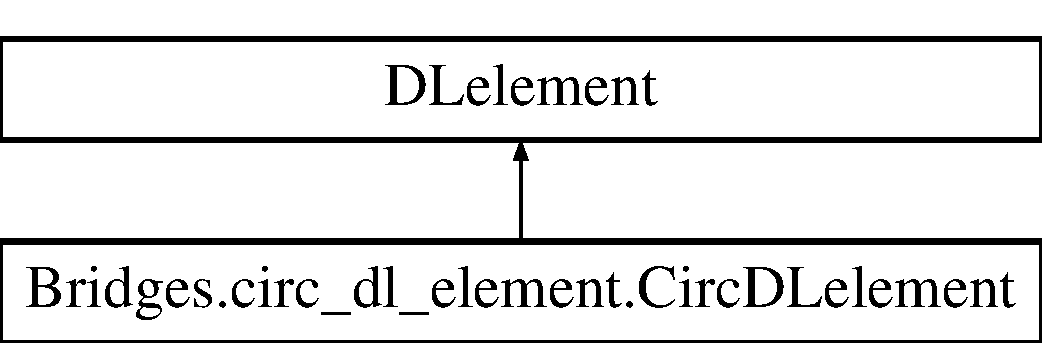
\includegraphics[height=2.000000cm]{class_bridges_1_1circ__dl__element_1_1_circ_d_lelement}
\end{center}
\end{figure}
\subsection*{Public Member Functions}
\begin{DoxyCompactItemize}
\item 
def \hyperlink{class_bridges_1_1circ__dl__element_1_1_circ_d_lelement_a79664a7230a1c2a55f69ea14f3216512}{\+\_\+\+\_\+init\+\_\+\+\_\+}
\begin{DoxyCompactList}\small\item\em Constructs an empty \hyperlink{class_bridges_1_1circ__dl__element_1_1_circ_d_lelement}{Circ\+D\+Lelement} with next and prev pointers set to itself. \end{DoxyCompactList}\item 
def \hyperlink{class_bridges_1_1circ__dl__element_1_1_circ_d_lelement_a47f182e2b4548acc63021b019ec09dd3}{get\+\_\+data\+\_\+structure\+\_\+type} (self)
\begin{DoxyCompactList}\small\item\em This method gets the data structure type. \end{DoxyCompactList}\item 
def \hyperlink{class_bridges_1_1circ__dl__element_1_1_circ_d_lelement_a5d52715940d44ce54de49948f55d5991}{get\+\_\+next} (self)
\begin{DoxyCompactList}\small\item\em This method returns the pointer to the next D\+Lelement. \end{DoxyCompactList}\item 
def \hyperlink{class_bridges_1_1circ__dl__element_1_1_circ_d_lelement_a1acacbb379727183540f705a48e95500}{get\+\_\+prev} (self)
\begin{DoxyCompactList}\small\item\em This method returns the pointer to the previous D\+Lelement. \end{DoxyCompactList}\end{DoxyCompactItemize}
\subsection*{Public Attributes}
\begin{DoxyCompactItemize}
\item 
\hyperlink{class_bridges_1_1circ__dl__element_1_1_circ_d_lelement_ab22d3f07990637d468acfb7dd47bf905}{next}
\item 
\hyperlink{class_bridges_1_1circ__dl__element_1_1_circ_d_lelement_ac52bcf8fb0ce64dfcda81007643510ab}{prev}
\end{DoxyCompactItemize}


\subsection{Detailed Description}
This class can be used to instantiate Circular Doubly Linked List Elements. 

Structurally they are the same as doubly linked elements except that each node constructed with the next and the previous pointers points to itself.

User\textquotesingle{}s implementation of the circularly linked list needs to ensure that the last node\textquotesingle{}s next pointer points to the first node and the first node\textquotesingle{}s previous pointer points to the last node, as the visualization generation is dependent on this.

Elements have labels (string) that are displayed on the visualization. Elements take an generic object E as a user defined parameter, which can be any native type or object.

Elements contain a visualizer (Element\+Visualizer) object for setting visual attributes (color, shape, opacity, size), necessary for displaying them in a web browser.

Elements also have a Link\+Visualizer object that is used when they are linked to another element, appropriate for setting link attributes, between the element and its previous or next nodes.

\begin{DoxyAuthor}{Author}
Kalpathi Subramanian
\end{DoxyAuthor}
\begin{DoxyDate}{Date}
7/17/16, 1/16/17 
\end{DoxyDate}


\subsection{Constructor \& Destructor Documentation}
\hypertarget{class_bridges_1_1circ__dl__element_1_1_circ_d_lelement_a79664a7230a1c2a55f69ea14f3216512}{}\index{Bridges\+::circ\+\_\+dl\+\_\+element\+::\+Circ\+D\+Lelement@{Bridges\+::circ\+\_\+dl\+\_\+element\+::\+Circ\+D\+Lelement}!\+\_\+\+\_\+init\+\_\+\+\_\+@{\+\_\+\+\_\+init\+\_\+\+\_\+}}
\index{\+\_\+\+\_\+init\+\_\+\+\_\+@{\+\_\+\+\_\+init\+\_\+\+\_\+}!Bridges\+::circ\+\_\+dl\+\_\+element\+::\+Circ\+D\+Lelement@{Bridges\+::circ\+\_\+dl\+\_\+element\+::\+Circ\+D\+Lelement}}
\subsubsection[{\+\_\+\+\_\+init\+\_\+\+\_\+}]{\setlength{\rightskip}{0pt plus 5cm}def Bridges.\+circ\+\_\+dl\+\_\+element.\+Circ\+D\+Lelement.\+\_\+\+\_\+init\+\_\+\+\_\+ (
\begin{DoxyParamCaption}
\item[{}]{self, }
\item[{}]{e = {\ttfamily None}, }
\item[{}]{label = {\ttfamily None}, }
\item[{}]{next = {\ttfamily None}, }
\item[{}]{prev = {\ttfamily None}}
\end{DoxyParamCaption}
)}\label{class_bridges_1_1circ__dl__element_1_1_circ_d_lelement_a79664a7230a1c2a55f69ea14f3216512}


Constructs an empty \hyperlink{class_bridges_1_1circ__dl__element_1_1_circ_d_lelement}{Circ\+D\+Lelement} with next and prev pointers set to itself. 


\begin{DoxyParams}{Parameters}
{\em label} & the label for this \hyperlink{class_bridges_1_1circ__dl__element_1_1_circ_d_lelement}{Circ\+D\+Lelement} \\
\hline
{\em e} & the genereic object that this \hyperlink{class_bridges_1_1circ__dl__element_1_1_circ_d_lelement}{Circ\+D\+Lelement} is holding \\
\hline
{\em next} & the D\+Lelement that should be assigned to the next pointer \\
\hline
{\em prev} & the D\+Lelement that should be assigned to the prev pointer \\
\hline
\end{DoxyParams}


\subsection{Member Function Documentation}
\hypertarget{class_bridges_1_1circ__dl__element_1_1_circ_d_lelement_a47f182e2b4548acc63021b019ec09dd3}{}\index{Bridges\+::circ\+\_\+dl\+\_\+element\+::\+Circ\+D\+Lelement@{Bridges\+::circ\+\_\+dl\+\_\+element\+::\+Circ\+D\+Lelement}!get\+\_\+data\+\_\+structure\+\_\+type@{get\+\_\+data\+\_\+structure\+\_\+type}}
\index{get\+\_\+data\+\_\+structure\+\_\+type@{get\+\_\+data\+\_\+structure\+\_\+type}!Bridges\+::circ\+\_\+dl\+\_\+element\+::\+Circ\+D\+Lelement@{Bridges\+::circ\+\_\+dl\+\_\+element\+::\+Circ\+D\+Lelement}}
\subsubsection[{get\+\_\+data\+\_\+structure\+\_\+type(self)}]{\setlength{\rightskip}{0pt plus 5cm}def Bridges.\+circ\+\_\+dl\+\_\+element.\+Circ\+D\+Lelement.\+get\+\_\+data\+\_\+structure\+\_\+type (
\begin{DoxyParamCaption}
\item[{}]{self}
\end{DoxyParamCaption}
)}\label{class_bridges_1_1circ__dl__element_1_1_circ_d_lelement_a47f182e2b4548acc63021b019ec09dd3}


This method gets the data structure type. 

\begin{DoxyReturn}{Returns}
The date structure type as a string 
\end{DoxyReturn}
\hypertarget{class_bridges_1_1circ__dl__element_1_1_circ_d_lelement_a5d52715940d44ce54de49948f55d5991}{}\index{Bridges\+::circ\+\_\+dl\+\_\+element\+::\+Circ\+D\+Lelement@{Bridges\+::circ\+\_\+dl\+\_\+element\+::\+Circ\+D\+Lelement}!get\+\_\+next@{get\+\_\+next}}
\index{get\+\_\+next@{get\+\_\+next}!Bridges\+::circ\+\_\+dl\+\_\+element\+::\+Circ\+D\+Lelement@{Bridges\+::circ\+\_\+dl\+\_\+element\+::\+Circ\+D\+Lelement}}
\subsubsection[{get\+\_\+next(self)}]{\setlength{\rightskip}{0pt plus 5cm}def Bridges.\+circ\+\_\+dl\+\_\+element.\+Circ\+D\+Lelement.\+get\+\_\+next (
\begin{DoxyParamCaption}
\item[{}]{self}
\end{DoxyParamCaption}
)}\label{class_bridges_1_1circ__dl__element_1_1_circ_d_lelement_a5d52715940d44ce54de49948f55d5991}


This method returns the pointer to the next D\+Lelement. 

\begin{DoxyReturn}{Returns}
the D\+Lelement assigned to the next pointer 
\end{DoxyReturn}
\hypertarget{class_bridges_1_1circ__dl__element_1_1_circ_d_lelement_a1acacbb379727183540f705a48e95500}{}\index{Bridges\+::circ\+\_\+dl\+\_\+element\+::\+Circ\+D\+Lelement@{Bridges\+::circ\+\_\+dl\+\_\+element\+::\+Circ\+D\+Lelement}!get\+\_\+prev@{get\+\_\+prev}}
\index{get\+\_\+prev@{get\+\_\+prev}!Bridges\+::circ\+\_\+dl\+\_\+element\+::\+Circ\+D\+Lelement@{Bridges\+::circ\+\_\+dl\+\_\+element\+::\+Circ\+D\+Lelement}}
\subsubsection[{get\+\_\+prev(self)}]{\setlength{\rightskip}{0pt plus 5cm}def Bridges.\+circ\+\_\+dl\+\_\+element.\+Circ\+D\+Lelement.\+get\+\_\+prev (
\begin{DoxyParamCaption}
\item[{}]{self}
\end{DoxyParamCaption}
)}\label{class_bridges_1_1circ__dl__element_1_1_circ_d_lelement_a1acacbb379727183540f705a48e95500}


This method returns the pointer to the previous D\+Lelement. 

\begin{DoxyReturn}{Returns}
the D\+Lelement assigned to the prev pointer 
\end{DoxyReturn}


\subsection{Member Data Documentation}
\hypertarget{class_bridges_1_1circ__dl__element_1_1_circ_d_lelement_ab22d3f07990637d468acfb7dd47bf905}{}\index{Bridges\+::circ\+\_\+dl\+\_\+element\+::\+Circ\+D\+Lelement@{Bridges\+::circ\+\_\+dl\+\_\+element\+::\+Circ\+D\+Lelement}!next@{next}}
\index{next@{next}!Bridges\+::circ\+\_\+dl\+\_\+element\+::\+Circ\+D\+Lelement@{Bridges\+::circ\+\_\+dl\+\_\+element\+::\+Circ\+D\+Lelement}}
\subsubsection[{next}]{\setlength{\rightskip}{0pt plus 5cm}Bridges.\+circ\+\_\+dl\+\_\+element.\+Circ\+D\+Lelement.\+next}\label{class_bridges_1_1circ__dl__element_1_1_circ_d_lelement_ab22d3f07990637d468acfb7dd47bf905}
\hypertarget{class_bridges_1_1circ__dl__element_1_1_circ_d_lelement_ac52bcf8fb0ce64dfcda81007643510ab}{}\index{Bridges\+::circ\+\_\+dl\+\_\+element\+::\+Circ\+D\+Lelement@{Bridges\+::circ\+\_\+dl\+\_\+element\+::\+Circ\+D\+Lelement}!prev@{prev}}
\index{prev@{prev}!Bridges\+::circ\+\_\+dl\+\_\+element\+::\+Circ\+D\+Lelement@{Bridges\+::circ\+\_\+dl\+\_\+element\+::\+Circ\+D\+Lelement}}
\subsubsection[{prev}]{\setlength{\rightskip}{0pt plus 5cm}Bridges.\+circ\+\_\+dl\+\_\+element.\+Circ\+D\+Lelement.\+prev}\label{class_bridges_1_1circ__dl__element_1_1_circ_d_lelement_ac52bcf8fb0ce64dfcda81007643510ab}


The documentation for this class was generated from the following file\+:\begin{DoxyCompactItemize}
\item 
/\+Users/kalpathi/gr/bridges/client/python/\+Bridges/\hyperlink{circ__dl__element_8py}{circ\+\_\+dl\+\_\+element.\+py}\end{DoxyCompactItemize}

\hypertarget{class_bridges_1_1circle_1_1_circle}{}\section{Bridges.\+circle.\+Circle Class Reference}
\label{class_bridges_1_1circle_1_1_circle}\index{Bridges.\+circle.\+Circle@{Bridges.\+circle.\+Circle}}
Inheritance diagram for Bridges.\+circle.\+Circle\+:\begin{figure}[H]
\begin{center}
\leavevmode
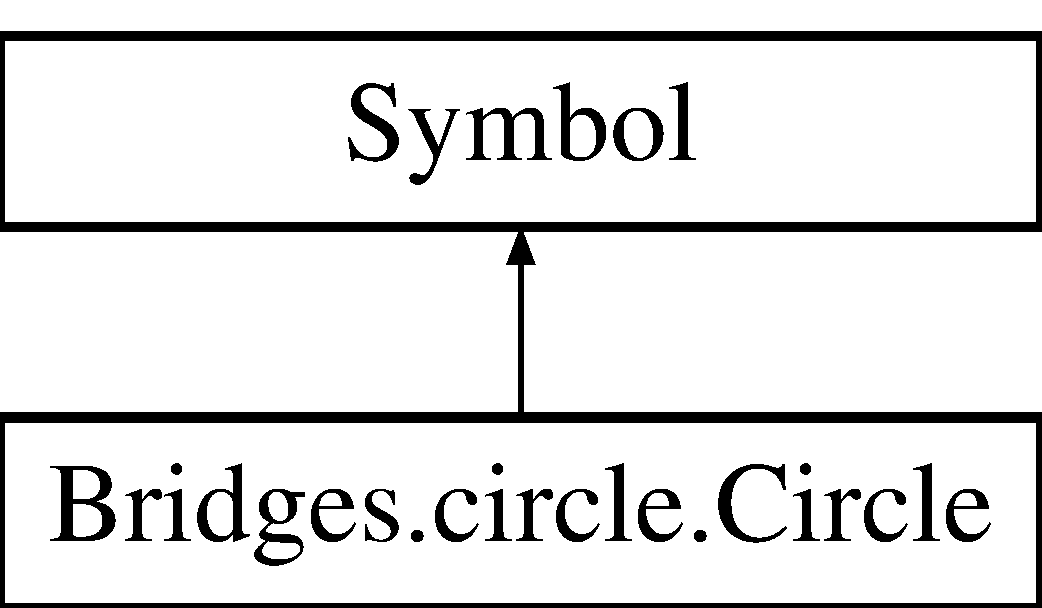
\includegraphics[height=2.000000cm]{class_bridges_1_1circle_1_1_circle}
\end{center}
\end{figure}
\subsection*{Public Member Functions}
\begin{DoxyCompactItemize}
\item 
def \mbox{\hyperlink{class_bridges_1_1circle_1_1_circle_a0e2f0eba0cfdf7dc1119a0002eddcea5}{\+\_\+\+\_\+init\+\_\+\+\_\+}} (self, locx=None, locy=None, r=None)
\item 
def \mbox{\hyperlink{class_bridges_1_1circle_1_1_circle_a3a60ae8fe94fdedde07cbf8d02e024cc}{get\+\_\+name}} (self)
\item 
def \mbox{\hyperlink{class_bridges_1_1circle_1_1_circle_a14f3e3923d9a73a7bb68d0be793c9f32}{set\+\_\+radius}} (self, r)
\item 
def \mbox{\hyperlink{class_bridges_1_1circle_1_1_circle_a85792b4c4382baa5812f98a43457e1de}{set\+\_\+circle}} (self, locx, locy, r)
\item 
def \mbox{\hyperlink{class_bridges_1_1circle_1_1_circle_af7e5541a823ca0a3341eac9a8f78d97b}{get\+\_\+dimensions}} (self)
\item 
def \mbox{\hyperlink{class_bridges_1_1circle_1_1_circle_a85089832e547f5b8755ba2c37bc0e7b3}{get\+\_\+json\+\_\+representation}} (self)
\end{DoxyCompactItemize}
\subsection*{Public Attributes}
\begin{DoxyCompactItemize}
\item 
\mbox{\hyperlink{class_bridges_1_1circle_1_1_circle_acd92a71e93a265ad2679935b007f279f}{radius}}
\end{DoxyCompactItemize}


\subsection{Constructor \& Destructor Documentation}
\mbox{\Hypertarget{class_bridges_1_1circle_1_1_circle_a0e2f0eba0cfdf7dc1119a0002eddcea5}\label{class_bridges_1_1circle_1_1_circle_a0e2f0eba0cfdf7dc1119a0002eddcea5}} 
\index{Bridges\+::circle\+::\+Circle@{Bridges\+::circle\+::\+Circle}!\+\_\+\+\_\+init\+\_\+\+\_\+@{\+\_\+\+\_\+init\+\_\+\+\_\+}}
\index{\+\_\+\+\_\+init\+\_\+\+\_\+@{\+\_\+\+\_\+init\+\_\+\+\_\+}!Bridges\+::circle\+::\+Circle@{Bridges\+::circle\+::\+Circle}}
\subsubsection{\texorpdfstring{\+\_\+\+\_\+init\+\_\+\+\_\+()}{\_\_init\_\_()}}
{\footnotesize\ttfamily def Bridges.\+circle.\+Circle.\+\_\+\+\_\+init\+\_\+\+\_\+ (\begin{DoxyParamCaption}\item[{}]{self,  }\item[{}]{locx = {\ttfamily None},  }\item[{}]{locy = {\ttfamily None},  }\item[{}]{r = {\ttfamily None} }\end{DoxyParamCaption})}



\subsection{Member Function Documentation}
\mbox{\Hypertarget{class_bridges_1_1circle_1_1_circle_af7e5541a823ca0a3341eac9a8f78d97b}\label{class_bridges_1_1circle_1_1_circle_af7e5541a823ca0a3341eac9a8f78d97b}} 
\index{Bridges\+::circle\+::\+Circle@{Bridges\+::circle\+::\+Circle}!get\+\_\+dimensions@{get\+\_\+dimensions}}
\index{get\+\_\+dimensions@{get\+\_\+dimensions}!Bridges\+::circle\+::\+Circle@{Bridges\+::circle\+::\+Circle}}
\subsubsection{\texorpdfstring{get\+\_\+dimensions()}{get\_dimensions()}}
{\footnotesize\ttfamily def Bridges.\+circle.\+Circle.\+get\+\_\+dimensions (\begin{DoxyParamCaption}\item[{}]{self }\end{DoxyParamCaption})}

\mbox{\Hypertarget{class_bridges_1_1circle_1_1_circle_a85089832e547f5b8755ba2c37bc0e7b3}\label{class_bridges_1_1circle_1_1_circle_a85089832e547f5b8755ba2c37bc0e7b3}} 
\index{Bridges\+::circle\+::\+Circle@{Bridges\+::circle\+::\+Circle}!get\+\_\+json\+\_\+representation@{get\+\_\+json\+\_\+representation}}
\index{get\+\_\+json\+\_\+representation@{get\+\_\+json\+\_\+representation}!Bridges\+::circle\+::\+Circle@{Bridges\+::circle\+::\+Circle}}
\subsubsection{\texorpdfstring{get\+\_\+json\+\_\+representation()}{get\_json\_representation()}}
{\footnotesize\ttfamily def Bridges.\+circle.\+Circle.\+get\+\_\+json\+\_\+representation (\begin{DoxyParamCaption}\item[{}]{self }\end{DoxyParamCaption})}

\mbox{\Hypertarget{class_bridges_1_1circle_1_1_circle_a3a60ae8fe94fdedde07cbf8d02e024cc}\label{class_bridges_1_1circle_1_1_circle_a3a60ae8fe94fdedde07cbf8d02e024cc}} 
\index{Bridges\+::circle\+::\+Circle@{Bridges\+::circle\+::\+Circle}!get\+\_\+name@{get\+\_\+name}}
\index{get\+\_\+name@{get\+\_\+name}!Bridges\+::circle\+::\+Circle@{Bridges\+::circle\+::\+Circle}}
\subsubsection{\texorpdfstring{get\+\_\+name()}{get\_name()}}
{\footnotesize\ttfamily def Bridges.\+circle.\+Circle.\+get\+\_\+name (\begin{DoxyParamCaption}\item[{}]{self }\end{DoxyParamCaption})}

\mbox{\Hypertarget{class_bridges_1_1circle_1_1_circle_a85792b4c4382baa5812f98a43457e1de}\label{class_bridges_1_1circle_1_1_circle_a85792b4c4382baa5812f98a43457e1de}} 
\index{Bridges\+::circle\+::\+Circle@{Bridges\+::circle\+::\+Circle}!set\+\_\+circle@{set\+\_\+circle}}
\index{set\+\_\+circle@{set\+\_\+circle}!Bridges\+::circle\+::\+Circle@{Bridges\+::circle\+::\+Circle}}
\subsubsection{\texorpdfstring{set\+\_\+circle()}{set\_circle()}}
{\footnotesize\ttfamily def Bridges.\+circle.\+Circle.\+set\+\_\+circle (\begin{DoxyParamCaption}\item[{}]{self,  }\item[{}]{locx,  }\item[{}]{locy,  }\item[{}]{r }\end{DoxyParamCaption})}

\mbox{\Hypertarget{class_bridges_1_1circle_1_1_circle_a14f3e3923d9a73a7bb68d0be793c9f32}\label{class_bridges_1_1circle_1_1_circle_a14f3e3923d9a73a7bb68d0be793c9f32}} 
\index{Bridges\+::circle\+::\+Circle@{Bridges\+::circle\+::\+Circle}!set\+\_\+radius@{set\+\_\+radius}}
\index{set\+\_\+radius@{set\+\_\+radius}!Bridges\+::circle\+::\+Circle@{Bridges\+::circle\+::\+Circle}}
\subsubsection{\texorpdfstring{set\+\_\+radius()}{set\_radius()}}
{\footnotesize\ttfamily def Bridges.\+circle.\+Circle.\+set\+\_\+radius (\begin{DoxyParamCaption}\item[{}]{self,  }\item[{}]{r }\end{DoxyParamCaption})}



\subsection{Member Data Documentation}
\mbox{\Hypertarget{class_bridges_1_1circle_1_1_circle_acd92a71e93a265ad2679935b007f279f}\label{class_bridges_1_1circle_1_1_circle_acd92a71e93a265ad2679935b007f279f}} 
\index{Bridges\+::circle\+::\+Circle@{Bridges\+::circle\+::\+Circle}!radius@{radius}}
\index{radius@{radius}!Bridges\+::circle\+::\+Circle@{Bridges\+::circle\+::\+Circle}}
\subsubsection{\texorpdfstring{radius}{radius}}
{\footnotesize\ttfamily Bridges.\+circle.\+Circle.\+radius}



The documentation for this class was generated from the following file\+:\begin{DoxyCompactItemize}
\item 
/\+Users/kalpathi/gr/bridges/client/python/bridges18/\+Bridges/\mbox{\hyperlink{circle_8py}{circle.\+py}}\end{DoxyCompactItemize}

\hypertarget{class_bridges_1_1circ__sl__element_1_1_circ_s_lelement}{}\section{Bridges.\+circ\+\_\+sl\+\_\+element.\+Circ\+S\+Lelement Class Reference}
\label{class_bridges_1_1circ__sl__element_1_1_circ_s_lelement}\index{Bridges.\+circ\+\_\+sl\+\_\+element.\+Circ\+S\+Lelement@{Bridges.\+circ\+\_\+sl\+\_\+element.\+Circ\+S\+Lelement}}


This class can be used to instantiate Singly Linked Circular List Elements.  


Inheritance diagram for Bridges.\+circ\+\_\+sl\+\_\+element.\+Circ\+S\+Lelement\+:\begin{figure}[H]
\begin{center}
\leavevmode
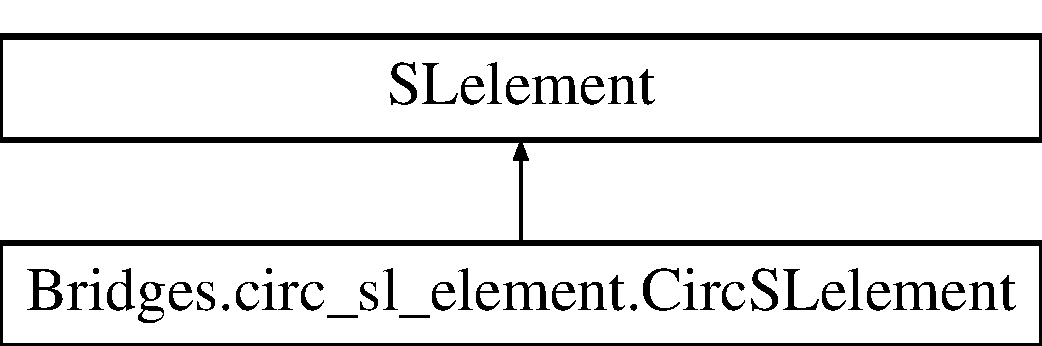
\includegraphics[height=2.000000cm]{class_bridges_1_1circ__sl__element_1_1_circ_s_lelement}
\end{center}
\end{figure}
\subsection*{Public Member Functions}
\begin{DoxyCompactItemize}
\item 
def \hyperlink{class_bridges_1_1circ__sl__element_1_1_circ_s_lelement_a6f1b38f5f3350a4c8d280e938cec3662}{\+\_\+\+\_\+init\+\_\+\+\_\+}
\begin{DoxyCompactList}\small\item\em This constructor creates an \hyperlink{class_bridges_1_1circ__sl__element_1_1_circ_s_lelement}{Circ\+S\+Lelement} object and sets its next pointer to itself. \end{DoxyCompactList}\item 
def \hyperlink{class_bridges_1_1circ__sl__element_1_1_circ_s_lelement_a53774e23afd83780f1a8a64a68892494}{get\+\_\+data\+\_\+structure\+\_\+type} (self)
\begin{DoxyCompactList}\small\item\em This method gets the data structure type. \end{DoxyCompactList}\item 
def \hyperlink{class_bridges_1_1circ__sl__element_1_1_circ_s_lelement_a709b68b1e016734f15c64bde94077d58}{get\+\_\+next} (self)
\begin{DoxyCompactList}\small\item\em Retrieves the next \hyperlink{class_bridges_1_1circ__sl__element_1_1_circ_s_lelement}{Circ\+S\+Lelement}. \end{DoxyCompactList}\item 
def \hyperlink{class_bridges_1_1circ__sl__element_1_1_circ_s_lelement_ab19b10a71d5f93996eb15c19cfaf2688}{\+\_\+\+\_\+str\+\_\+\+\_\+} (self)
\end{DoxyCompactItemize}


\subsection{Detailed Description}
This class can be used to instantiate Singly Linked Circular List Elements. 

Structurally they are the same as singly linked elements except that each node constructed with the next point pointing to itself; User\textquotesingle{}s implementation of the circularly linked list needs to ensure that the last node points to first node of the list, as the visualization generation is dependent on this.

Elements have labels (string) that are displayed on the visualization. Elements take an generic object as a user defined parameter, E, which can be any native type or object.

Elements contains a visualizer (Element\+Visualizer) object for setting visual attributes (color, shape, opacity, size), necessary for displaying them in a web browser.

Elements also have a Link\+Visualizer object that is used when they are linked to another element, appropriate for setting link attributes, between an element and its next element.

\begin{DoxyAuthor}{Author}
Kalpathi Subramanian
\end{DoxyAuthor}
\begin{DoxyDate}{Date}
6/22/16, 1/7/17, 5/17/17 
\end{DoxyDate}


\subsection{Constructor \& Destructor Documentation}
\hypertarget{class_bridges_1_1circ__sl__element_1_1_circ_s_lelement_a6f1b38f5f3350a4c8d280e938cec3662}{}\index{Bridges\+::circ\+\_\+sl\+\_\+element\+::\+Circ\+S\+Lelement@{Bridges\+::circ\+\_\+sl\+\_\+element\+::\+Circ\+S\+Lelement}!\+\_\+\+\_\+init\+\_\+\+\_\+@{\+\_\+\+\_\+init\+\_\+\+\_\+}}
\index{\+\_\+\+\_\+init\+\_\+\+\_\+@{\+\_\+\+\_\+init\+\_\+\+\_\+}!Bridges\+::circ\+\_\+sl\+\_\+element\+::\+Circ\+S\+Lelement@{Bridges\+::circ\+\_\+sl\+\_\+element\+::\+Circ\+S\+Lelement}}
\subsubsection[{\+\_\+\+\_\+init\+\_\+\+\_\+}]{\setlength{\rightskip}{0pt plus 5cm}def Bridges.\+circ\+\_\+sl\+\_\+element.\+Circ\+S\+Lelement.\+\_\+\+\_\+init\+\_\+\+\_\+ (
\begin{DoxyParamCaption}
\item[{}]{self, }
\item[{}]{e = {\ttfamily None}, }
\item[{}]{label = {\ttfamily None}, }
\item[{}]{next = {\ttfamily None}}
\end{DoxyParamCaption}
)}\label{class_bridges_1_1circ__sl__element_1_1_circ_s_lelement_a6f1b38f5f3350a4c8d280e938cec3662}


This constructor creates an \hyperlink{class_bridges_1_1circ__sl__element_1_1_circ_s_lelement}{Circ\+S\+Lelement} object and sets its next pointer to itself. 


\begin{DoxyParams}{Parameters}
{\em label} & the label of \hyperlink{class_bridges_1_1circ__sl__element_1_1_circ_s_lelement}{Circ\+S\+Lelement} \\
\hline
{\em e} & the generic object that this \hyperlink{class_bridges_1_1circ__sl__element_1_1_circ_s_lelement}{Circ\+S\+Lelement} will hold \\
\hline
{\em next} & the \hyperlink{class_bridges_1_1circ__sl__element_1_1_circ_s_lelement}{Circ\+S\+Lelement} that should be assigned to the next pointer \\
\hline
\end{DoxyParams}


\subsection{Member Function Documentation}
\hypertarget{class_bridges_1_1circ__sl__element_1_1_circ_s_lelement_ab19b10a71d5f93996eb15c19cfaf2688}{}\index{Bridges\+::circ\+\_\+sl\+\_\+element\+::\+Circ\+S\+Lelement@{Bridges\+::circ\+\_\+sl\+\_\+element\+::\+Circ\+S\+Lelement}!\+\_\+\+\_\+str\+\_\+\+\_\+@{\+\_\+\+\_\+str\+\_\+\+\_\+}}
\index{\+\_\+\+\_\+str\+\_\+\+\_\+@{\+\_\+\+\_\+str\+\_\+\+\_\+}!Bridges\+::circ\+\_\+sl\+\_\+element\+::\+Circ\+S\+Lelement@{Bridges\+::circ\+\_\+sl\+\_\+element\+::\+Circ\+S\+Lelement}}
\subsubsection[{\+\_\+\+\_\+str\+\_\+\+\_\+(self)}]{\setlength{\rightskip}{0pt plus 5cm}def Bridges.\+circ\+\_\+sl\+\_\+element.\+Circ\+S\+Lelement.\+\_\+\+\_\+str\+\_\+\+\_\+ (
\begin{DoxyParamCaption}
\item[{}]{self}
\end{DoxyParamCaption}
)}\label{class_bridges_1_1circ__sl__element_1_1_circ_s_lelement_ab19b10a71d5f93996eb15c19cfaf2688}
\hypertarget{class_bridges_1_1circ__sl__element_1_1_circ_s_lelement_a53774e23afd83780f1a8a64a68892494}{}\index{Bridges\+::circ\+\_\+sl\+\_\+element\+::\+Circ\+S\+Lelement@{Bridges\+::circ\+\_\+sl\+\_\+element\+::\+Circ\+S\+Lelement}!get\+\_\+data\+\_\+structure\+\_\+type@{get\+\_\+data\+\_\+structure\+\_\+type}}
\index{get\+\_\+data\+\_\+structure\+\_\+type@{get\+\_\+data\+\_\+structure\+\_\+type}!Bridges\+::circ\+\_\+sl\+\_\+element\+::\+Circ\+S\+Lelement@{Bridges\+::circ\+\_\+sl\+\_\+element\+::\+Circ\+S\+Lelement}}
\subsubsection[{get\+\_\+data\+\_\+structure\+\_\+type(self)}]{\setlength{\rightskip}{0pt plus 5cm}def Bridges.\+circ\+\_\+sl\+\_\+element.\+Circ\+S\+Lelement.\+get\+\_\+data\+\_\+structure\+\_\+type (
\begin{DoxyParamCaption}
\item[{}]{self}
\end{DoxyParamCaption}
)}\label{class_bridges_1_1circ__sl__element_1_1_circ_s_lelement_a53774e23afd83780f1a8a64a68892494}


This method gets the data structure type. 

\begin{DoxyReturn}{Returns}
The date structure type as a string 
\end{DoxyReturn}
\hypertarget{class_bridges_1_1circ__sl__element_1_1_circ_s_lelement_a709b68b1e016734f15c64bde94077d58}{}\index{Bridges\+::circ\+\_\+sl\+\_\+element\+::\+Circ\+S\+Lelement@{Bridges\+::circ\+\_\+sl\+\_\+element\+::\+Circ\+S\+Lelement}!get\+\_\+next@{get\+\_\+next}}
\index{get\+\_\+next@{get\+\_\+next}!Bridges\+::circ\+\_\+sl\+\_\+element\+::\+Circ\+S\+Lelement@{Bridges\+::circ\+\_\+sl\+\_\+element\+::\+Circ\+S\+Lelement}}
\subsubsection[{get\+\_\+next(self)}]{\setlength{\rightskip}{0pt plus 5cm}def Bridges.\+circ\+\_\+sl\+\_\+element.\+Circ\+S\+Lelement.\+get\+\_\+next (
\begin{DoxyParamCaption}
\item[{}]{self}
\end{DoxyParamCaption}
)}\label{class_bridges_1_1circ__sl__element_1_1_circ_s_lelement_a709b68b1e016734f15c64bde94077d58}


Retrieves the next \hyperlink{class_bridges_1_1circ__sl__element_1_1_circ_s_lelement}{Circ\+S\+Lelement}. 

\begin{DoxyReturn}{Returns}
Circ\+S\+Lelement$<$\+E$>$ assigned to next 
\end{DoxyReturn}


The documentation for this class was generated from the following file\+:\begin{DoxyCompactItemize}
\item 
/\+Users/kalpathi/gr/bridges/client/python/\+Bridges/\hyperlink{circ__sl__element_8py}{circ\+\_\+sl\+\_\+element.\+py}\end{DoxyCompactItemize}

\hypertarget{class_bridges_1_1color_1_1_color}{}\section{Bridges.\+color.\+Color Class Reference}
\label{class_bridges_1_1color_1_1_color}\index{Bridges.\+color.\+Color@{Bridges.\+color.\+Color}}
Inheritance diagram for Bridges.\+color.\+Color\+:\begin{figure}[H]
\begin{center}
\leavevmode
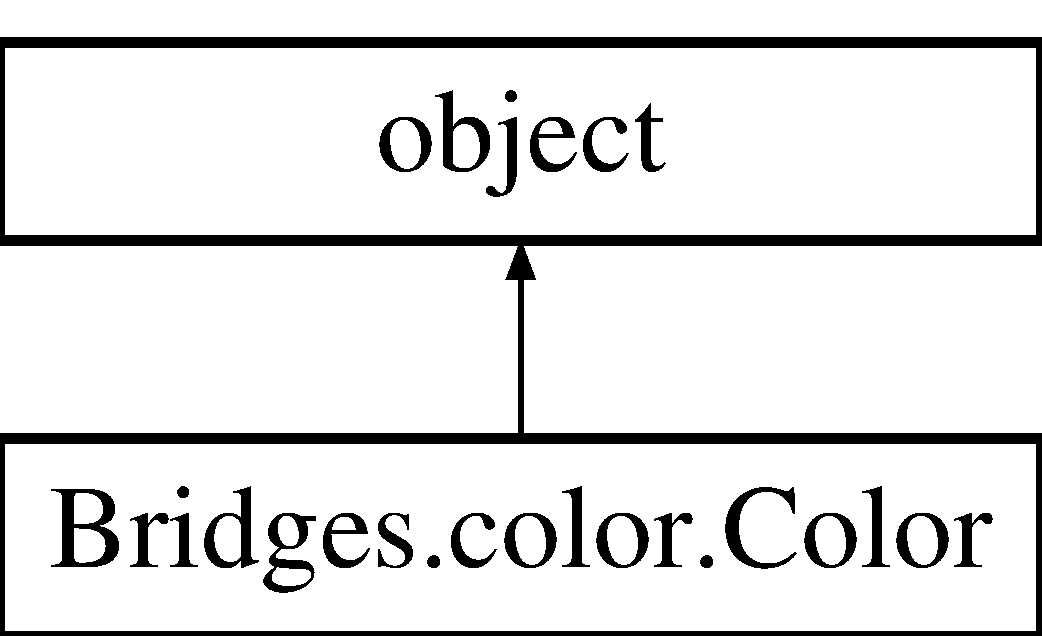
\includegraphics[height=2.000000cm]{class_bridges_1_1color_1_1_color}
\end{center}
\end{figure}
\subsection*{Public Member Functions}
\begin{DoxyCompactItemize}
\item 
def \mbox{\hyperlink{class_bridges_1_1color_1_1_color_ae89e14c5811e5bfd8812ea5aae98c60c}{red}} (self)
\item 
def \mbox{\hyperlink{class_bridges_1_1color_1_1_color_adc4ac7f0a6c24c58e83e243a8e4a92f6}{red}}
\item 
def \mbox{\hyperlink{class_bridges_1_1color_1_1_color_ae89e14c5811e5bfd8812ea5aae98c60c}{red}} (self)
\item 
def \mbox{\hyperlink{class_bridges_1_1color_1_1_color_a0fd6bbb5c35a59dce498c459df18a6c1}{green}} (self)
\item 
def \mbox{\hyperlink{class_bridges_1_1color_1_1_color_aa212c2e85ebb0a91db7ef3a957121d7e}{green}}
\item 
def \mbox{\hyperlink{class_bridges_1_1color_1_1_color_a0fd6bbb5c35a59dce498c459df18a6c1}{green}} (self)
\item 
def \mbox{\hyperlink{class_bridges_1_1color_1_1_color_a0c7174e0cc79f94bba0378e80afd416b}{blue}} (self)
\item 
def \mbox{\hyperlink{class_bridges_1_1color_1_1_color_ae13a368cd4278e676227526afe69c1ad}{blue}}
\item 
def \mbox{\hyperlink{class_bridges_1_1color_1_1_color_a0c7174e0cc79f94bba0378e80afd416b}{blue}} (self)
\item 
def \mbox{\hyperlink{class_bridges_1_1color_1_1_color_a4c9ef08c6ca50f58d6b581dbba1d7ff5}{alpha}} (self)
\item 
def \mbox{\hyperlink{class_bridges_1_1color_1_1_color_aee0ad3b65052fdd4b7b25388463764ee}{alpha}}
\item 
def \mbox{\hyperlink{class_bridges_1_1color_1_1_color_a4c9ef08c6ca50f58d6b581dbba1d7ff5}{alpha}} (self)
\item 
def \mbox{\hyperlink{class_bridges_1_1color_1_1_color_a31b443f464eb5e7218ff5bd001161d2b}{rgba}} (self, int, int, int, float)
\item 
def \mbox{\hyperlink{class_bridges_1_1color_1_1_color_adfbba0839dbf564ef5befb8f19b26fdf}{rgba}}
\item 
def \mbox{\hyperlink{class_bridges_1_1color_1_1_color_aac259c3e0639eb257f8a5959d7e1ed2f}{rgba}} (self)
\item 
def \mbox{\hyperlink{class_bridges_1_1color_1_1_color_ab66face8abc6657a93f5c0ed05911994}{\+\_\+\+\_\+init\+\_\+\+\_\+}} (self, args, kwargs)
\item 
def \mbox{\hyperlink{class_bridges_1_1color_1_1_color_a747d78b7ff8981b1f93749bd53aeab7b}{set\+\_\+color}} (self, args, kwargs)
\item 
def \mbox{\hyperlink{class_bridges_1_1color_1_1_color_abecd67f51c2a564993027a70eea7a8e4}{set\+\_\+red}}
\item 
def \mbox{\hyperlink{class_bridges_1_1color_1_1_color_a1b6e88d20dc472eb03739811856d8cb8}{get\+\_\+red}} (self)
\item 
def \mbox{\hyperlink{class_bridges_1_1color_1_1_color_ab6f15725fa7f2290c325a808a487b3dd}{set\+\_\+green}}
\item 
def \mbox{\hyperlink{class_bridges_1_1color_1_1_color_ad4395417f67ab98115dbe61f50f82ac3}{get\+\_\+green}} (self)
\item 
def \mbox{\hyperlink{class_bridges_1_1color_1_1_color_a8e3fff5331750fed91062795fccaddde}{set\+\_\+blue}}
\item 
def \mbox{\hyperlink{class_bridges_1_1color_1_1_color_a8cd38cbd71134b56485dcbaa146f220d}{get\+\_\+blue}} (self)
\item 
def \mbox{\hyperlink{class_bridges_1_1color_1_1_color_acbfa06efd60c3d5eb003a2d254a23c04}{set\+\_\+alpha}}
\item 
def \mbox{\hyperlink{class_bridges_1_1color_1_1_color_a48fe3bb99a272e283f836790b9c49465}{get\+\_\+alpha}} (self)
\item 
def \mbox{\hyperlink{class_bridges_1_1color_1_1_color_a4456ca2aea18e6018c932df15c041040}{get\+\_\+byte\+\_\+representation}} (self)
\item 
def \mbox{\hyperlink{class_bridges_1_1color_1_1_color_a46bc7ca0a13c2c3152a81d82593fee7e}{\+\_\+\+\_\+eq\+\_\+\+\_\+}} (self, other)
\end{DoxyCompactItemize}
\subsection*{Public Attributes}
\begin{DoxyCompactItemize}
\item 
\mbox{\hyperlink{class_bridges_1_1color_1_1_color_a4074ee82f60039f1964c9c92049d12f2}{alpha}}
\item 
\mbox{\hyperlink{class_bridges_1_1color_1_1_color_a25663f2be911b45eea32c70a24ef983b}{red}}
\item 
\mbox{\hyperlink{class_bridges_1_1color_1_1_color_ac7b1d3a34feecde69b5437214ff83895}{green}}
\item 
\mbox{\hyperlink{class_bridges_1_1color_1_1_color_ab3eb91c32b56dcb17fc9315706439137}{blue}}
\end{DoxyCompactItemize}


\subsection{Detailed Description}
\begin{DoxyVerb}This class is used to represent colors in bridges.

We use and RGBA model to represent colors, with the Red Green and Blue components ranging from 0-255,
with the alpha ranging from 0.0-1.0 inclusive.

We use webcolors to handle color names passed to the constructor/set_color function.
https://webcolors.readthedocs.io/en/1.8.1/
All CSS3 color names should be valid:
https://developer.mozilla.org/en-US/docs/Web/CSS/color_value
https://www.w3.org/TR/css-color-3/#svg-color

Attributes:
    red (int): red component of color ranging from 0-255 inclusive (default 0)
    green (int): green component of color ranging from 0-255 inclusive (default 0)
    blue (int): blue component of color ranging from 0-255 inclusive (default 0)
    alpha (float): alpha component of color ranging from 0.0-1.0 inclusive (default 1.0)
    rgba (tuple(int, int, int, alpha)): RGBA components as respective tuple
Args:
    args: int, int, int, Optional(float) or a str as singular arg
    kwargs:
        r or red: Optional(int)
        b or blue: Optional(int)
        g or green: Optional(int)
        a or alpha: Optional(float)
        col_name: Optional(str)
Raises:
    ValueError: if args is not 3 ints with an optional 4th arg for alpha or just one str arg
    ValueError: if a str passed is not a valid webcolor
    ValueError: if any of the RGBA values are outside of their respective range
Examples:
    >>> my_color = Color("red")
    >>> my_color.rgba
    (255, 0, 0, 1.0)
    >>> my_color = Color(r=255)
    >>> my_color.rgba
    (255, 0, 0, 1.0)
    >>> my_color = Color(255, 0, 0)
    >>> my_color.rgba
    (255, 0, 0, 1.0)
    >>> my_color = Color()
    >>> my_color.red = 255
    >>> my_color.rgba
    (255, 0, 0, 1.0)
\end{DoxyVerb}
 

\subsection{Constructor \& Destructor Documentation}
\mbox{\Hypertarget{class_bridges_1_1color_1_1_color_ab66face8abc6657a93f5c0ed05911994}\label{class_bridges_1_1color_1_1_color_ab66face8abc6657a93f5c0ed05911994}} 
\index{Bridges\+::color\+::\+Color@{Bridges\+::color\+::\+Color}!\+\_\+\+\_\+init\+\_\+\+\_\+@{\+\_\+\+\_\+init\+\_\+\+\_\+}}
\index{\+\_\+\+\_\+init\+\_\+\+\_\+@{\+\_\+\+\_\+init\+\_\+\+\_\+}!Bridges\+::color\+::\+Color@{Bridges\+::color\+::\+Color}}
\subsubsection{\texorpdfstring{\+\_\+\+\_\+init\+\_\+\+\_\+()}{\_\_init\_\_()}}
{\footnotesize\ttfamily def Bridges.\+color.\+Color.\+\_\+\+\_\+init\+\_\+\+\_\+ (\begin{DoxyParamCaption}\item[{}]{self,  }\item[{}]{args,  }\item[{}]{kwargs }\end{DoxyParamCaption})}

\begin{DoxyVerb}Constructor for a Color object
Usage: requires either 3 ints 0-255 for RGB and an optional float 0.0-1.0 for alpha or a str of a web color
can also key the RGBA values with r, g, b, a or red, green, blue, alpha respectively and col_name for the str
:param args: int, int, int, optional float or just a str
:param kwargs: r/red: int, b/blue: int, g/green: int optional a/alpha: float or col_name: str
:return: None
\end{DoxyVerb}
 

\subsection{Member Function Documentation}
\mbox{\Hypertarget{class_bridges_1_1color_1_1_color_a46bc7ca0a13c2c3152a81d82593fee7e}\label{class_bridges_1_1color_1_1_color_a46bc7ca0a13c2c3152a81d82593fee7e}} 
\index{Bridges\+::color\+::\+Color@{Bridges\+::color\+::\+Color}!\+\_\+\+\_\+eq\+\_\+\+\_\+@{\+\_\+\+\_\+eq\+\_\+\+\_\+}}
\index{\+\_\+\+\_\+eq\+\_\+\+\_\+@{\+\_\+\+\_\+eq\+\_\+\+\_\+}!Bridges\+::color\+::\+Color@{Bridges\+::color\+::\+Color}}
\subsubsection{\texorpdfstring{\+\_\+\+\_\+eq\+\_\+\+\_\+()}{\_\_eq\_\_()}}
{\footnotesize\ttfamily def Bridges.\+color.\+Color.\+\_\+\+\_\+eq\+\_\+\+\_\+ (\begin{DoxyParamCaption}\item[{}]{self,  }\item[{}]{other }\end{DoxyParamCaption})}

\begin{DoxyVerb}deep equality check, by value of each RGBA value\end{DoxyVerb}
 \mbox{\Hypertarget{class_bridges_1_1color_1_1_color_a4c9ef08c6ca50f58d6b581dbba1d7ff5}\label{class_bridges_1_1color_1_1_color_a4c9ef08c6ca50f58d6b581dbba1d7ff5}} 
\index{Bridges\+::color\+::\+Color@{Bridges\+::color\+::\+Color}!alpha@{alpha}}
\index{alpha@{alpha}!Bridges\+::color\+::\+Color@{Bridges\+::color\+::\+Color}}
\subsubsection{\texorpdfstring{alpha()}{alpha()}\hspace{0.1cm}{\footnotesize\ttfamily [1/3]}}
{\footnotesize\ttfamily def Bridges.\+color.\+Color.\+alpha (\begin{DoxyParamCaption}\item[{}]{self,  }\item[{}]{float }\end{DoxyParamCaption})}

\begin{DoxyVerb}alpha component of color
:return float: alpha component of color
Must be a value between 0.0-1.0 inclusive
\end{DoxyVerb}
 \mbox{\Hypertarget{class_bridges_1_1color_1_1_color_aee0ad3b65052fdd4b7b25388463764ee}\label{class_bridges_1_1color_1_1_color_aee0ad3b65052fdd4b7b25388463764ee}} 
\index{Bridges\+::color\+::\+Color@{Bridges\+::color\+::\+Color}!alpha@{alpha}}
\index{alpha@{alpha}!Bridges\+::color\+::\+Color@{Bridges\+::color\+::\+Color}}
\subsubsection{\texorpdfstring{alpha()}{alpha()}\hspace{0.1cm}{\footnotesize\ttfamily [2/3]}}
{\footnotesize\ttfamily def Bridges.\+color.\+Color.\+alpha (\begin{DoxyParamCaption}\item[{}]{self,  }\item[{}]{value }\end{DoxyParamCaption})}

\mbox{\Hypertarget{class_bridges_1_1color_1_1_color_a4c9ef08c6ca50f58d6b581dbba1d7ff5}\label{class_bridges_1_1color_1_1_color_a4c9ef08c6ca50f58d6b581dbba1d7ff5}} 
\index{Bridges\+::color\+::\+Color@{Bridges\+::color\+::\+Color}!alpha@{alpha}}
\index{alpha@{alpha}!Bridges\+::color\+::\+Color@{Bridges\+::color\+::\+Color}}
\subsubsection{\texorpdfstring{alpha()}{alpha()}\hspace{0.1cm}{\footnotesize\ttfamily [3/3]}}
{\footnotesize\ttfamily def Bridges.\+color.\+Color.\+alpha (\begin{DoxyParamCaption}\item[{}]{self }\end{DoxyParamCaption})}

\mbox{\Hypertarget{class_bridges_1_1color_1_1_color_a0c7174e0cc79f94bba0378e80afd416b}\label{class_bridges_1_1color_1_1_color_a0c7174e0cc79f94bba0378e80afd416b}} 
\index{Bridges\+::color\+::\+Color@{Bridges\+::color\+::\+Color}!blue@{blue}}
\index{blue@{blue}!Bridges\+::color\+::\+Color@{Bridges\+::color\+::\+Color}}
\subsubsection{\texorpdfstring{blue()}{blue()}\hspace{0.1cm}{\footnotesize\ttfamily [1/3]}}
{\footnotesize\ttfamily def Bridges.\+color.\+Color.\+blue (\begin{DoxyParamCaption}\item[{}]{self,  }\item[{}]{int }\end{DoxyParamCaption})}

\begin{DoxyVerb}blue component of color
:return int: blue component of color
Must be a value between 0-255 inclusive
\end{DoxyVerb}
 \mbox{\Hypertarget{class_bridges_1_1color_1_1_color_ae13a368cd4278e676227526afe69c1ad}\label{class_bridges_1_1color_1_1_color_ae13a368cd4278e676227526afe69c1ad}} 
\index{Bridges\+::color\+::\+Color@{Bridges\+::color\+::\+Color}!blue@{blue}}
\index{blue@{blue}!Bridges\+::color\+::\+Color@{Bridges\+::color\+::\+Color}}
\subsubsection{\texorpdfstring{blue()}{blue()}\hspace{0.1cm}{\footnotesize\ttfamily [2/3]}}
{\footnotesize\ttfamily def Bridges.\+color.\+Color.\+blue (\begin{DoxyParamCaption}\item[{}]{self,  }\item[{}]{value }\end{DoxyParamCaption})}

\mbox{\Hypertarget{class_bridges_1_1color_1_1_color_a0c7174e0cc79f94bba0378e80afd416b}\label{class_bridges_1_1color_1_1_color_a0c7174e0cc79f94bba0378e80afd416b}} 
\index{Bridges\+::color\+::\+Color@{Bridges\+::color\+::\+Color}!blue@{blue}}
\index{blue@{blue}!Bridges\+::color\+::\+Color@{Bridges\+::color\+::\+Color}}
\subsubsection{\texorpdfstring{blue()}{blue()}\hspace{0.1cm}{\footnotesize\ttfamily [3/3]}}
{\footnotesize\ttfamily def Bridges.\+color.\+Color.\+blue (\begin{DoxyParamCaption}\item[{}]{self }\end{DoxyParamCaption})}

\mbox{\Hypertarget{class_bridges_1_1color_1_1_color_a48fe3bb99a272e283f836790b9c49465}\label{class_bridges_1_1color_1_1_color_a48fe3bb99a272e283f836790b9c49465}} 
\index{Bridges\+::color\+::\+Color@{Bridges\+::color\+::\+Color}!get\+\_\+alpha@{get\+\_\+alpha}}
\index{get\+\_\+alpha@{get\+\_\+alpha}!Bridges\+::color\+::\+Color@{Bridges\+::color\+::\+Color}}
\subsubsection{\texorpdfstring{get\+\_\+alpha()}{get\_alpha()}}
{\footnotesize\ttfamily def Bridges.\+color.\+Color.\+get\+\_\+alpha (\begin{DoxyParamCaption}\item[{}]{self,  }\item[{}]{float }\end{DoxyParamCaption})}

\begin{DoxyVerb}:return float: alpha component of color\end{DoxyVerb}
 \mbox{\Hypertarget{class_bridges_1_1color_1_1_color_a8cd38cbd71134b56485dcbaa146f220d}\label{class_bridges_1_1color_1_1_color_a8cd38cbd71134b56485dcbaa146f220d}} 
\index{Bridges\+::color\+::\+Color@{Bridges\+::color\+::\+Color}!get\+\_\+blue@{get\+\_\+blue}}
\index{get\+\_\+blue@{get\+\_\+blue}!Bridges\+::color\+::\+Color@{Bridges\+::color\+::\+Color}}
\subsubsection{\texorpdfstring{get\+\_\+blue()}{get\_blue()}}
{\footnotesize\ttfamily def Bridges.\+color.\+Color.\+get\+\_\+blue (\begin{DoxyParamCaption}\item[{}]{self,  }\item[{}]{int }\end{DoxyParamCaption})}

\begin{DoxyVerb}":return int: blue component of color\end{DoxyVerb}
 \mbox{\Hypertarget{class_bridges_1_1color_1_1_color_a4456ca2aea18e6018c932df15c041040}\label{class_bridges_1_1color_1_1_color_a4456ca2aea18e6018c932df15c041040}} 
\index{Bridges\+::color\+::\+Color@{Bridges\+::color\+::\+Color}!get\+\_\+byte\+\_\+representation@{get\+\_\+byte\+\_\+representation}}
\index{get\+\_\+byte\+\_\+representation@{get\+\_\+byte\+\_\+representation}!Bridges\+::color\+::\+Color@{Bridges\+::color\+::\+Color}}
\subsubsection{\texorpdfstring{get\+\_\+byte\+\_\+representation()}{get\_byte\_representation()}}
{\footnotesize\ttfamily def Bridges.\+color.\+Color.\+get\+\_\+byte\+\_\+representation (\begin{DoxyParamCaption}\item[{}]{self,  }\item[{}]{list }\end{DoxyParamCaption})}

\begin{DoxyVerb}:return list(int):RGBA values as list of ints from 0-255\end{DoxyVerb}
 \mbox{\Hypertarget{class_bridges_1_1color_1_1_color_ad4395417f67ab98115dbe61f50f82ac3}\label{class_bridges_1_1color_1_1_color_ad4395417f67ab98115dbe61f50f82ac3}} 
\index{Bridges\+::color\+::\+Color@{Bridges\+::color\+::\+Color}!get\+\_\+green@{get\+\_\+green}}
\index{get\+\_\+green@{get\+\_\+green}!Bridges\+::color\+::\+Color@{Bridges\+::color\+::\+Color}}
\subsubsection{\texorpdfstring{get\+\_\+green()}{get\_green()}}
{\footnotesize\ttfamily def Bridges.\+color.\+Color.\+get\+\_\+green (\begin{DoxyParamCaption}\item[{}]{self,  }\item[{}]{int }\end{DoxyParamCaption})}

\begin{DoxyVerb}:return int: green component of color\end{DoxyVerb}
 \mbox{\Hypertarget{class_bridges_1_1color_1_1_color_a1b6e88d20dc472eb03739811856d8cb8}\label{class_bridges_1_1color_1_1_color_a1b6e88d20dc472eb03739811856d8cb8}} 
\index{Bridges\+::color\+::\+Color@{Bridges\+::color\+::\+Color}!get\+\_\+red@{get\+\_\+red}}
\index{get\+\_\+red@{get\+\_\+red}!Bridges\+::color\+::\+Color@{Bridges\+::color\+::\+Color}}
\subsubsection{\texorpdfstring{get\+\_\+red()}{get\_red()}}
{\footnotesize\ttfamily def Bridges.\+color.\+Color.\+get\+\_\+red (\begin{DoxyParamCaption}\item[{}]{self,  }\item[{}]{int }\end{DoxyParamCaption})}

\begin{DoxyVerb}:return int: red component of color\end{DoxyVerb}
 \mbox{\Hypertarget{class_bridges_1_1color_1_1_color_a0fd6bbb5c35a59dce498c459df18a6c1}\label{class_bridges_1_1color_1_1_color_a0fd6bbb5c35a59dce498c459df18a6c1}} 
\index{Bridges\+::color\+::\+Color@{Bridges\+::color\+::\+Color}!green@{green}}
\index{green@{green}!Bridges\+::color\+::\+Color@{Bridges\+::color\+::\+Color}}
\subsubsection{\texorpdfstring{green()}{green()}\hspace{0.1cm}{\footnotesize\ttfamily [1/3]}}
{\footnotesize\ttfamily def Bridges.\+color.\+Color.\+green (\begin{DoxyParamCaption}\item[{}]{self,  }\item[{}]{int }\end{DoxyParamCaption})}

\begin{DoxyVerb}green component of color
:return int: green component of color
Must be a value between 0-255 inclusive
\end{DoxyVerb}
 \mbox{\Hypertarget{class_bridges_1_1color_1_1_color_aa212c2e85ebb0a91db7ef3a957121d7e}\label{class_bridges_1_1color_1_1_color_aa212c2e85ebb0a91db7ef3a957121d7e}} 
\index{Bridges\+::color\+::\+Color@{Bridges\+::color\+::\+Color}!green@{green}}
\index{green@{green}!Bridges\+::color\+::\+Color@{Bridges\+::color\+::\+Color}}
\subsubsection{\texorpdfstring{green()}{green()}\hspace{0.1cm}{\footnotesize\ttfamily [2/3]}}
{\footnotesize\ttfamily def Bridges.\+color.\+Color.\+green (\begin{DoxyParamCaption}\item[{}]{self,  }\item[{}]{value }\end{DoxyParamCaption})}

\mbox{\Hypertarget{class_bridges_1_1color_1_1_color_a0fd6bbb5c35a59dce498c459df18a6c1}\label{class_bridges_1_1color_1_1_color_a0fd6bbb5c35a59dce498c459df18a6c1}} 
\index{Bridges\+::color\+::\+Color@{Bridges\+::color\+::\+Color}!green@{green}}
\index{green@{green}!Bridges\+::color\+::\+Color@{Bridges\+::color\+::\+Color}}
\subsubsection{\texorpdfstring{green()}{green()}\hspace{0.1cm}{\footnotesize\ttfamily [3/3]}}
{\footnotesize\ttfamily def Bridges.\+color.\+Color.\+green (\begin{DoxyParamCaption}\item[{}]{self }\end{DoxyParamCaption})}

\mbox{\Hypertarget{class_bridges_1_1color_1_1_color_ae89e14c5811e5bfd8812ea5aae98c60c}\label{class_bridges_1_1color_1_1_color_ae89e14c5811e5bfd8812ea5aae98c60c}} 
\index{Bridges\+::color\+::\+Color@{Bridges\+::color\+::\+Color}!red@{red}}
\index{red@{red}!Bridges\+::color\+::\+Color@{Bridges\+::color\+::\+Color}}
\subsubsection{\texorpdfstring{red()}{red()}\hspace{0.1cm}{\footnotesize\ttfamily [1/3]}}
{\footnotesize\ttfamily def Bridges.\+color.\+Color.\+red (\begin{DoxyParamCaption}\item[{}]{self,  }\item[{}]{int }\end{DoxyParamCaption})}

\begin{DoxyVerb}red component of color
:return int: red component of color
Must be a value between 0-255 inclusive
\end{DoxyVerb}
 \mbox{\Hypertarget{class_bridges_1_1color_1_1_color_adc4ac7f0a6c24c58e83e243a8e4a92f6}\label{class_bridges_1_1color_1_1_color_adc4ac7f0a6c24c58e83e243a8e4a92f6}} 
\index{Bridges\+::color\+::\+Color@{Bridges\+::color\+::\+Color}!red@{red}}
\index{red@{red}!Bridges\+::color\+::\+Color@{Bridges\+::color\+::\+Color}}
\subsubsection{\texorpdfstring{red()}{red()}\hspace{0.1cm}{\footnotesize\ttfamily [2/3]}}
{\footnotesize\ttfamily def Bridges.\+color.\+Color.\+red (\begin{DoxyParamCaption}\item[{}]{self,  }\item[{}]{value }\end{DoxyParamCaption})}

\mbox{\Hypertarget{class_bridges_1_1color_1_1_color_ae89e14c5811e5bfd8812ea5aae98c60c}\label{class_bridges_1_1color_1_1_color_ae89e14c5811e5bfd8812ea5aae98c60c}} 
\index{Bridges\+::color\+::\+Color@{Bridges\+::color\+::\+Color}!red@{red}}
\index{red@{red}!Bridges\+::color\+::\+Color@{Bridges\+::color\+::\+Color}}
\subsubsection{\texorpdfstring{red()}{red()}\hspace{0.1cm}{\footnotesize\ttfamily [3/3]}}
{\footnotesize\ttfamily def Bridges.\+color.\+Color.\+red (\begin{DoxyParamCaption}\item[{}]{self }\end{DoxyParamCaption})}

\mbox{\Hypertarget{class_bridges_1_1color_1_1_color_a31b443f464eb5e7218ff5bd001161d2b}\label{class_bridges_1_1color_1_1_color_a31b443f464eb5e7218ff5bd001161d2b}} 
\index{Bridges\+::color\+::\+Color@{Bridges\+::color\+::\+Color}!rgba@{rgba}}
\index{rgba@{rgba}!Bridges\+::color\+::\+Color@{Bridges\+::color\+::\+Color}}
\subsubsection{\texorpdfstring{rgba()}{rgba()}\hspace{0.1cm}{\footnotesize\ttfamily [1/3]}}
{\footnotesize\ttfamily def Bridges.\+color.\+Color.\+rgba (\begin{DoxyParamCaption}\item[{}]{self,  }\item[{}]{int,  }\item[{}]{int,  }\item[{}]{int,  }\item[{}]{float }\end{DoxyParamCaption})}

\begin{DoxyVerb}RGBA components as respective tuple
Represents the RGBA values of the color as a tuple, can be used to set or get all values at once
:return (int, int, int, float): RGBA values respectively
\end{DoxyVerb}
 \mbox{\Hypertarget{class_bridges_1_1color_1_1_color_adfbba0839dbf564ef5befb8f19b26fdf}\label{class_bridges_1_1color_1_1_color_adfbba0839dbf564ef5befb8f19b26fdf}} 
\index{Bridges\+::color\+::\+Color@{Bridges\+::color\+::\+Color}!rgba@{rgba}}
\index{rgba@{rgba}!Bridges\+::color\+::\+Color@{Bridges\+::color\+::\+Color}}
\subsubsection{\texorpdfstring{rgba()}{rgba()}\hspace{0.1cm}{\footnotesize\ttfamily [2/3]}}
{\footnotesize\ttfamily def Bridges.\+color.\+Color.\+rgba (\begin{DoxyParamCaption}\item[{}]{self,  }\item[{}]{rgba }\end{DoxyParamCaption})}

\mbox{\Hypertarget{class_bridges_1_1color_1_1_color_aac259c3e0639eb257f8a5959d7e1ed2f}\label{class_bridges_1_1color_1_1_color_aac259c3e0639eb257f8a5959d7e1ed2f}} 
\index{Bridges\+::color\+::\+Color@{Bridges\+::color\+::\+Color}!rgba@{rgba}}
\index{rgba@{rgba}!Bridges\+::color\+::\+Color@{Bridges\+::color\+::\+Color}}
\subsubsection{\texorpdfstring{rgba()}{rgba()}\hspace{0.1cm}{\footnotesize\ttfamily [3/3]}}
{\footnotesize\ttfamily def Bridges.\+color.\+Color.\+rgba (\begin{DoxyParamCaption}\item[{}]{self }\end{DoxyParamCaption})}

\mbox{\Hypertarget{class_bridges_1_1color_1_1_color_acbfa06efd60c3d5eb003a2d254a23c04}\label{class_bridges_1_1color_1_1_color_acbfa06efd60c3d5eb003a2d254a23c04}} 
\index{Bridges\+::color\+::\+Color@{Bridges\+::color\+::\+Color}!set\+\_\+alpha@{set\+\_\+alpha}}
\index{set\+\_\+alpha@{set\+\_\+alpha}!Bridges\+::color\+::\+Color@{Bridges\+::color\+::\+Color}}
\subsubsection{\texorpdfstring{set\+\_\+alpha()}{set\_alpha()}}
{\footnotesize\ttfamily def Bridges.\+color.\+Color.\+set\+\_\+alpha (\begin{DoxyParamCaption}\item[{}]{self,  }\item[{}]{a }\end{DoxyParamCaption})}

\mbox{\Hypertarget{class_bridges_1_1color_1_1_color_a8e3fff5331750fed91062795fccaddde}\label{class_bridges_1_1color_1_1_color_a8e3fff5331750fed91062795fccaddde}} 
\index{Bridges\+::color\+::\+Color@{Bridges\+::color\+::\+Color}!set\+\_\+blue@{set\+\_\+blue}}
\index{set\+\_\+blue@{set\+\_\+blue}!Bridges\+::color\+::\+Color@{Bridges\+::color\+::\+Color}}
\subsubsection{\texorpdfstring{set\+\_\+blue()}{set\_blue()}}
{\footnotesize\ttfamily def Bridges.\+color.\+Color.\+set\+\_\+blue (\begin{DoxyParamCaption}\item[{}]{self,  }\item[{}]{b }\end{DoxyParamCaption})}

\mbox{\Hypertarget{class_bridges_1_1color_1_1_color_a747d78b7ff8981b1f93749bd53aeab7b}\label{class_bridges_1_1color_1_1_color_a747d78b7ff8981b1f93749bd53aeab7b}} 
\index{Bridges\+::color\+::\+Color@{Bridges\+::color\+::\+Color}!set\+\_\+color@{set\+\_\+color}}
\index{set\+\_\+color@{set\+\_\+color}!Bridges\+::color\+::\+Color@{Bridges\+::color\+::\+Color}}
\subsubsection{\texorpdfstring{set\+\_\+color()}{set\_color()}}
{\footnotesize\ttfamily def Bridges.\+color.\+Color.\+set\+\_\+color (\begin{DoxyParamCaption}\item[{}]{self,  }\item[{}]{args,  }\item[{}]{kwargs,  }\item[{}]{None }\end{DoxyParamCaption})}

\begin{DoxyVerb}Usage: requires either 3 ints 0-255 for RGB and an optional float 0.0-1.0 for alpha or a str of a web color
can also key the RGBA values with r, g, b, a or red, green, blue, alpha respectively and col_name for the str
:param args: int, int, int optional float or str
:param kwargs: r/red: int, b/blue: int, g/green: int optional a/alpha: float or col_name: str
:return: None
\end{DoxyVerb}
 \mbox{\Hypertarget{class_bridges_1_1color_1_1_color_ab6f15725fa7f2290c325a808a487b3dd}\label{class_bridges_1_1color_1_1_color_ab6f15725fa7f2290c325a808a487b3dd}} 
\index{Bridges\+::color\+::\+Color@{Bridges\+::color\+::\+Color}!set\+\_\+green@{set\+\_\+green}}
\index{set\+\_\+green@{set\+\_\+green}!Bridges\+::color\+::\+Color@{Bridges\+::color\+::\+Color}}
\subsubsection{\texorpdfstring{set\+\_\+green()}{set\_green()}}
{\footnotesize\ttfamily def Bridges.\+color.\+Color.\+set\+\_\+green (\begin{DoxyParamCaption}\item[{}]{self,  }\item[{}]{g }\end{DoxyParamCaption})}

\mbox{\Hypertarget{class_bridges_1_1color_1_1_color_abecd67f51c2a564993027a70eea7a8e4}\label{class_bridges_1_1color_1_1_color_abecd67f51c2a564993027a70eea7a8e4}} 
\index{Bridges\+::color\+::\+Color@{Bridges\+::color\+::\+Color}!set\+\_\+red@{set\+\_\+red}}
\index{set\+\_\+red@{set\+\_\+red}!Bridges\+::color\+::\+Color@{Bridges\+::color\+::\+Color}}
\subsubsection{\texorpdfstring{set\+\_\+red()}{set\_red()}}
{\footnotesize\ttfamily def Bridges.\+color.\+Color.\+set\+\_\+red (\begin{DoxyParamCaption}\item[{}]{self,  }\item[{}]{r }\end{DoxyParamCaption})}



\subsection{Member Data Documentation}
\mbox{\Hypertarget{class_bridges_1_1color_1_1_color_a4074ee82f60039f1964c9c92049d12f2}\label{class_bridges_1_1color_1_1_color_a4074ee82f60039f1964c9c92049d12f2}} 
\index{Bridges\+::color\+::\+Color@{Bridges\+::color\+::\+Color}!alpha@{alpha}}
\index{alpha@{alpha}!Bridges\+::color\+::\+Color@{Bridges\+::color\+::\+Color}}
\subsubsection{\texorpdfstring{alpha}{alpha}}
{\footnotesize\ttfamily Bridges.\+color.\+Color.\+alpha}

\mbox{\Hypertarget{class_bridges_1_1color_1_1_color_ab3eb91c32b56dcb17fc9315706439137}\label{class_bridges_1_1color_1_1_color_ab3eb91c32b56dcb17fc9315706439137}} 
\index{Bridges\+::color\+::\+Color@{Bridges\+::color\+::\+Color}!blue@{blue}}
\index{blue@{blue}!Bridges\+::color\+::\+Color@{Bridges\+::color\+::\+Color}}
\subsubsection{\texorpdfstring{blue}{blue}}
{\footnotesize\ttfamily Bridges.\+color.\+Color.\+blue}

\mbox{\Hypertarget{class_bridges_1_1color_1_1_color_ac7b1d3a34feecde69b5437214ff83895}\label{class_bridges_1_1color_1_1_color_ac7b1d3a34feecde69b5437214ff83895}} 
\index{Bridges\+::color\+::\+Color@{Bridges\+::color\+::\+Color}!green@{green}}
\index{green@{green}!Bridges\+::color\+::\+Color@{Bridges\+::color\+::\+Color}}
\subsubsection{\texorpdfstring{green}{green}}
{\footnotesize\ttfamily Bridges.\+color.\+Color.\+green}

\mbox{\Hypertarget{class_bridges_1_1color_1_1_color_a25663f2be911b45eea32c70a24ef983b}\label{class_bridges_1_1color_1_1_color_a25663f2be911b45eea32c70a24ef983b}} 
\index{Bridges\+::color\+::\+Color@{Bridges\+::color\+::\+Color}!red@{red}}
\index{red@{red}!Bridges\+::color\+::\+Color@{Bridges\+::color\+::\+Color}}
\subsubsection{\texorpdfstring{red}{red}}
{\footnotesize\ttfamily Bridges.\+color.\+Color.\+red}



The documentation for this class was generated from the following file\+:\begin{DoxyCompactItemize}
\item 
/\+Users/kalpathi/gr/bridges/client/python/bridges18/\+Bridges/\mbox{\hyperlink{color_8py}{color.\+py}}\end{DoxyCompactItemize}

\hypertarget{class_bridges_1_1color__grid_1_1_color_grid}{}\section{Bridges.\+color\+\_\+grid.\+Color\+Grid Class Reference}
\label{class_bridges_1_1color__grid_1_1_color_grid}\index{Bridges.\+color\+\_\+grid.\+Color\+Grid@{Bridges.\+color\+\_\+grid.\+Color\+Grid}}


This is a class in B\+R\+I\+D\+G\+E\+S for representing an (n x n) grid.  


Inheritance diagram for Bridges.\+color\+\_\+grid.\+Color\+Grid\+:\begin{figure}[H]
\begin{center}
\leavevmode
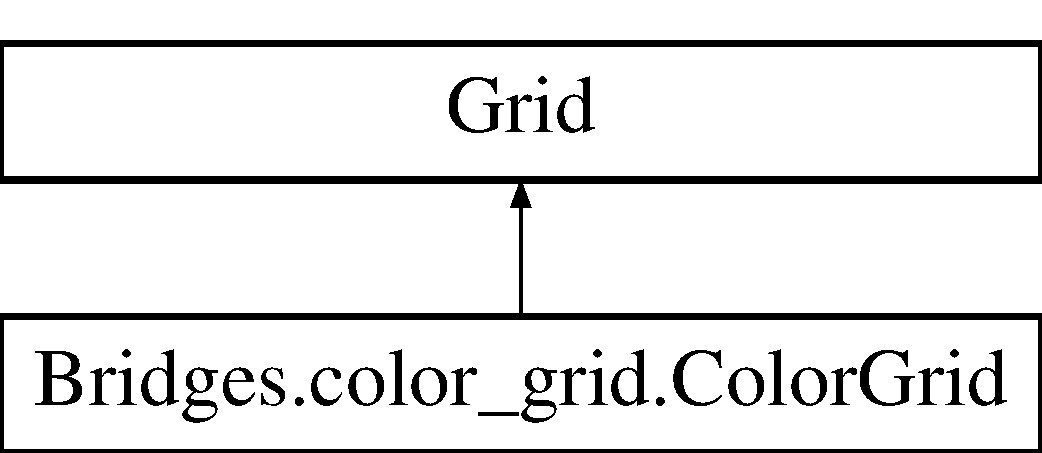
\includegraphics[height=2.000000cm]{class_bridges_1_1color__grid_1_1_color_grid}
\end{center}
\end{figure}
\subsection*{Public Member Functions}
\begin{DoxyCompactItemize}
\item 
def \hyperlink{class_bridges_1_1color__grid_1_1_color_grid_abd68c44e314544bcf6cc8b049bda480c}{get\+\_\+data\+\_\+structure\+\_\+type} (self)
\item 
def \hyperlink{class_bridges_1_1color__grid_1_1_color_grid_abb7ba6ff8fceda840957eeebc3fd6ad2}{\+\_\+\+\_\+init\+\_\+\+\_\+}
\item 
def \hyperlink{class_bridges_1_1color__grid_1_1_color_grid_ac6bbb13314c1947dbad31b8c2071ccdf}{initialize\+\_\+grid} (self)
\begin{DoxyCompactList}\small\item\em Populate the grid with the base color. \end{DoxyCompactList}\item 
def \hyperlink{class_bridges_1_1color__grid_1_1_color_grid_a888333bc201b75a30612c4b5bd15b1df}{set} (self, row, col, color)
\begin{DoxyCompactList}\small\item\em set the (row, col) element in the \hyperlink{class_bridges_1_1color__grid_1_1_color_grid}{Color\+Grid} \end{DoxyCompactList}\item 
def \hyperlink{class_bridges_1_1color__grid_1_1_color_grid_ab69a3b778c2127d3f7d30a23568bb046}{get\+\_\+rle} (self)
\begin{DoxyCompactList}\small\item\em get the Run Length Encoding of \hyperlink{class_bridges_1_1color__grid_1_1_color_grid}{Color\+Grid} \end{DoxyCompactList}\item 
def \hyperlink{class_bridges_1_1color__grid_1_1_color_grid_a6bf3130339641f4def29589a8175c066}{get\+\_\+raw} (self)
\begin{DoxyCompactList}\small\item\em get raw encoding of \hyperlink{class_bridges_1_1color__grid_1_1_color_grid}{Color\+Grid} \end{DoxyCompactList}\item 
def \hyperlink{class_bridges_1_1color__grid_1_1_color_grid_a8e235f55d0c97f3f5d7d0ab036ad7933}{get\+\_\+data\+\_\+structure\+\_\+representation} (self)
\begin{DoxyCompactList}\small\item\em get the J\+S\+O\+N representation of the color grid \end{DoxyCompactList}\end{DoxyCompactItemize}
\subsection*{Public Attributes}
\begin{DoxyCompactItemize}
\item 
\hyperlink{class_bridges_1_1color__grid_1_1_color_grid_a97e66f3c97bbf57c2aa2f5fb78c4114f}{base\+Color}
\item 
\hyperlink{class_bridges_1_1color__grid_1_1_color_grid_aabd8053e5acb920c28e519cd1ee69c35}{grid\+Size}
\end{DoxyCompactItemize}
\subsection*{Static Public Attributes}
\begin{DoxyCompactItemize}
\item 
string \hyperlink{class_bridges_1_1color__grid_1_1_color_grid_a1db881c79ab55a95c4c15dee31a1e431}{Q\+U\+O\+T\+E} = \char`\"{}\textbackslash{}\char`\"{}\char`\"{}
\item 
string \hyperlink{class_bridges_1_1color__grid_1_1_color_grid_af280f63885bffee3d3b6ecf0695844fc}{C\+O\+M\+M\+A} = \char`\"{},\char`\"{}
\item 
string \hyperlink{class_bridges_1_1color__grid_1_1_color_grid_a6185e36f338b56b33ff327afda157cf1}{C\+O\+L\+O\+N} = \char`\"{}\+:\char`\"{}
\item 
string \hyperlink{class_bridges_1_1color__grid_1_1_color_grid_a1f379a6c0e9fc4db2045e52678f15e20}{O\+P\+E\+N\+\_\+\+C\+U\+R\+L\+Y} = \char`\"{}\{\char`\"{}
\item 
string \hyperlink{class_bridges_1_1color__grid_1_1_color_grid_a05c0cee0f9ca312db59a1d60e53845ba}{C\+L\+O\+S\+E\+\_\+\+C\+U\+R\+L\+Y} = \char`\"{}\}\char`\"{}
\item 
string \hyperlink{class_bridges_1_1color__grid_1_1_color_grid_abde748d9ceae5339a3724b7064eee054}{O\+P\+E\+N\+\_\+\+P\+A\+R\+E\+N} = \char`\"{}(\char`\"{}
\item 
string \hyperlink{class_bridges_1_1color__grid_1_1_color_grid_afed081c42ad44319664d72567ee1b9ba}{C\+L\+O\+S\+E\+\_\+\+P\+A\+R\+E\+N} = \char`\"{})\char`\"{}
\item 
string \hyperlink{class_bridges_1_1color__grid_1_1_color_grid_a33869db1b3658c232827a2a0bc6e7170}{O\+P\+E\+N\+\_\+\+B\+O\+X} = \char`\"{}\mbox{[}\char`\"{}
\item 
string \hyperlink{class_bridges_1_1color__grid_1_1_color_grid_a9dcd6e3ce6c70a78216615edb35ec00e}{C\+L\+O\+S\+E\+\_\+\+B\+O\+X} = \char`\"{}\mbox{]}\char`\"{}
\item 
tuple \hyperlink{class_bridges_1_1color__grid_1_1_color_grid_a0bfaf5f4bdcf43899b67badca669e806}{base\+Color} = Color(r=0, g=0, b=0, a=1.\+0)
\end{DoxyCompactItemize}


\subsection{Detailed Description}
This is a class in B\+R\+I\+D\+G\+E\+S for representing an (n x n) grid. 

\begin{DoxyAuthor}{Author}
David Burlinson 
\end{DoxyAuthor}


\subsection{Constructor \& Destructor Documentation}
\hypertarget{class_bridges_1_1color__grid_1_1_color_grid_abb7ba6ff8fceda840957eeebc3fd6ad2}{}\index{Bridges\+::color\+\_\+grid\+::\+Color\+Grid@{Bridges\+::color\+\_\+grid\+::\+Color\+Grid}!\+\_\+\+\_\+init\+\_\+\+\_\+@{\+\_\+\+\_\+init\+\_\+\+\_\+}}
\index{\+\_\+\+\_\+init\+\_\+\+\_\+@{\+\_\+\+\_\+init\+\_\+\+\_\+}!Bridges\+::color\+\_\+grid\+::\+Color\+Grid@{Bridges\+::color\+\_\+grid\+::\+Color\+Grid}}
\subsubsection[{\+\_\+\+\_\+init\+\_\+\+\_\+}]{\setlength{\rightskip}{0pt plus 5cm}def Bridges.\+color\+\_\+grid.\+Color\+Grid.\+\_\+\+\_\+init\+\_\+\+\_\+ (
\begin{DoxyParamCaption}
\item[{}]{self, }
\item[{}]{rows}
\end{DoxyParamCaption}
)}\label{class_bridges_1_1color__grid_1_1_color_grid_abb7ba6ff8fceda840957eeebc3fd6ad2}


\subsection{Member Function Documentation}
\hypertarget{class_bridges_1_1color__grid_1_1_color_grid_a8e235f55d0c97f3f5d7d0ab036ad7933}{}\index{Bridges\+::color\+\_\+grid\+::\+Color\+Grid@{Bridges\+::color\+\_\+grid\+::\+Color\+Grid}!get\+\_\+data\+\_\+structure\+\_\+representation@{get\+\_\+data\+\_\+structure\+\_\+representation}}
\index{get\+\_\+data\+\_\+structure\+\_\+representation@{get\+\_\+data\+\_\+structure\+\_\+representation}!Bridges\+::color\+\_\+grid\+::\+Color\+Grid@{Bridges\+::color\+\_\+grid\+::\+Color\+Grid}}
\subsubsection[{get\+\_\+data\+\_\+structure\+\_\+representation(self)}]{\setlength{\rightskip}{0pt plus 5cm}def Bridges.\+color\+\_\+grid.\+Color\+Grid.\+get\+\_\+data\+\_\+structure\+\_\+representation (
\begin{DoxyParamCaption}
\item[{}]{self}
\end{DoxyParamCaption}
)}\label{class_bridges_1_1color__grid_1_1_color_grid_a8e235f55d0c97f3f5d7d0ab036ad7933}


get the J\+S\+O\+N representation of the color grid 

\begin{DoxyReturn}{Returns}
the J\+S\+O\+N representation of the color grid 
\end{DoxyReturn}
\hypertarget{class_bridges_1_1color__grid_1_1_color_grid_abd68c44e314544bcf6cc8b049bda480c}{}\index{Bridges\+::color\+\_\+grid\+::\+Color\+Grid@{Bridges\+::color\+\_\+grid\+::\+Color\+Grid}!get\+\_\+data\+\_\+structure\+\_\+type@{get\+\_\+data\+\_\+structure\+\_\+type}}
\index{get\+\_\+data\+\_\+structure\+\_\+type@{get\+\_\+data\+\_\+structure\+\_\+type}!Bridges\+::color\+\_\+grid\+::\+Color\+Grid@{Bridges\+::color\+\_\+grid\+::\+Color\+Grid}}
\subsubsection[{get\+\_\+data\+\_\+structure\+\_\+type(self)}]{\setlength{\rightskip}{0pt plus 5cm}def Bridges.\+color\+\_\+grid.\+Color\+Grid.\+get\+\_\+data\+\_\+structure\+\_\+type (
\begin{DoxyParamCaption}
\item[{}]{self}
\end{DoxyParamCaption}
)}\label{class_bridges_1_1color__grid_1_1_color_grid_abd68c44e314544bcf6cc8b049bda480c}
\hypertarget{class_bridges_1_1color__grid_1_1_color_grid_a6bf3130339641f4def29589a8175c066}{}\index{Bridges\+::color\+\_\+grid\+::\+Color\+Grid@{Bridges\+::color\+\_\+grid\+::\+Color\+Grid}!get\+\_\+raw@{get\+\_\+raw}}
\index{get\+\_\+raw@{get\+\_\+raw}!Bridges\+::color\+\_\+grid\+::\+Color\+Grid@{Bridges\+::color\+\_\+grid\+::\+Color\+Grid}}
\subsubsection[{get\+\_\+raw(self)}]{\setlength{\rightskip}{0pt plus 5cm}def Bridges.\+color\+\_\+grid.\+Color\+Grid.\+get\+\_\+raw (
\begin{DoxyParamCaption}
\item[{}]{self}
\end{DoxyParamCaption}
)}\label{class_bridges_1_1color__grid_1_1_color_grid_a6bf3130339641f4def29589a8175c066}


get raw encoding of \hyperlink{class_bridges_1_1color__grid_1_1_color_grid}{Color\+Grid} 

\hypertarget{class_bridges_1_1color__grid_1_1_color_grid_ab69a3b778c2127d3f7d30a23568bb046}{}\index{Bridges\+::color\+\_\+grid\+::\+Color\+Grid@{Bridges\+::color\+\_\+grid\+::\+Color\+Grid}!get\+\_\+rle@{get\+\_\+rle}}
\index{get\+\_\+rle@{get\+\_\+rle}!Bridges\+::color\+\_\+grid\+::\+Color\+Grid@{Bridges\+::color\+\_\+grid\+::\+Color\+Grid}}
\subsubsection[{get\+\_\+rle(self)}]{\setlength{\rightskip}{0pt plus 5cm}def Bridges.\+color\+\_\+grid.\+Color\+Grid.\+get\+\_\+rle (
\begin{DoxyParamCaption}
\item[{}]{self}
\end{DoxyParamCaption}
)}\label{class_bridges_1_1color__grid_1_1_color_grid_ab69a3b778c2127d3f7d30a23568bb046}


get the Run Length Encoding of \hyperlink{class_bridges_1_1color__grid_1_1_color_grid}{Color\+Grid} 

\hypertarget{class_bridges_1_1color__grid_1_1_color_grid_ac6bbb13314c1947dbad31b8c2071ccdf}{}\index{Bridges\+::color\+\_\+grid\+::\+Color\+Grid@{Bridges\+::color\+\_\+grid\+::\+Color\+Grid}!initialize\+\_\+grid@{initialize\+\_\+grid}}
\index{initialize\+\_\+grid@{initialize\+\_\+grid}!Bridges\+::color\+\_\+grid\+::\+Color\+Grid@{Bridges\+::color\+\_\+grid\+::\+Color\+Grid}}
\subsubsection[{initialize\+\_\+grid(self)}]{\setlength{\rightskip}{0pt plus 5cm}def Bridges.\+color\+\_\+grid.\+Color\+Grid.\+initialize\+\_\+grid (
\begin{DoxyParamCaption}
\item[{}]{self}
\end{DoxyParamCaption}
)}\label{class_bridges_1_1color__grid_1_1_color_grid_ac6bbb13314c1947dbad31b8c2071ccdf}


Populate the grid with the base color. 

\hypertarget{class_bridges_1_1color__grid_1_1_color_grid_a888333bc201b75a30612c4b5bd15b1df}{}\index{Bridges\+::color\+\_\+grid\+::\+Color\+Grid@{Bridges\+::color\+\_\+grid\+::\+Color\+Grid}!set@{set}}
\index{set@{set}!Bridges\+::color\+\_\+grid\+::\+Color\+Grid@{Bridges\+::color\+\_\+grid\+::\+Color\+Grid}}
\subsubsection[{set(self, row, col, color)}]{\setlength{\rightskip}{0pt plus 5cm}def Bridges.\+color\+\_\+grid.\+Color\+Grid.\+set (
\begin{DoxyParamCaption}
\item[{}]{self, }
\item[{}]{row, }
\item[{}]{col, }
\item[{}]{color}
\end{DoxyParamCaption}
)}\label{class_bridges_1_1color__grid_1_1_color_grid_a888333bc201b75a30612c4b5bd15b1df}


set the (row, col) element in the \hyperlink{class_bridges_1_1color__grid_1_1_color_grid}{Color\+Grid} 



\subsection{Member Data Documentation}
\hypertarget{class_bridges_1_1color__grid_1_1_color_grid_a0bfaf5f4bdcf43899b67badca669e806}{}\index{Bridges\+::color\+\_\+grid\+::\+Color\+Grid@{Bridges\+::color\+\_\+grid\+::\+Color\+Grid}!base\+Color@{base\+Color}}
\index{base\+Color@{base\+Color}!Bridges\+::color\+\_\+grid\+::\+Color\+Grid@{Bridges\+::color\+\_\+grid\+::\+Color\+Grid}}
\subsubsection[{base\+Color}]{\setlength{\rightskip}{0pt plus 5cm}tuple Bridges.\+color\+\_\+grid.\+Color\+Grid.\+base\+Color = Color(r=0, g=0, b=0, a=1.\+0)\hspace{0.3cm}{\ttfamily [static]}}\label{class_bridges_1_1color__grid_1_1_color_grid_a0bfaf5f4bdcf43899b67badca669e806}
\hypertarget{class_bridges_1_1color__grid_1_1_color_grid_a97e66f3c97bbf57c2aa2f5fb78c4114f}{}\index{Bridges\+::color\+\_\+grid\+::\+Color\+Grid@{Bridges\+::color\+\_\+grid\+::\+Color\+Grid}!base\+Color@{base\+Color}}
\index{base\+Color@{base\+Color}!Bridges\+::color\+\_\+grid\+::\+Color\+Grid@{Bridges\+::color\+\_\+grid\+::\+Color\+Grid}}
\subsubsection[{base\+Color}]{\setlength{\rightskip}{0pt plus 5cm}Bridges.\+color\+\_\+grid.\+Color\+Grid.\+base\+Color}\label{class_bridges_1_1color__grid_1_1_color_grid_a97e66f3c97bbf57c2aa2f5fb78c4114f}
\hypertarget{class_bridges_1_1color__grid_1_1_color_grid_a9dcd6e3ce6c70a78216615edb35ec00e}{}\index{Bridges\+::color\+\_\+grid\+::\+Color\+Grid@{Bridges\+::color\+\_\+grid\+::\+Color\+Grid}!C\+L\+O\+S\+E\+\_\+\+B\+O\+X@{C\+L\+O\+S\+E\+\_\+\+B\+O\+X}}
\index{C\+L\+O\+S\+E\+\_\+\+B\+O\+X@{C\+L\+O\+S\+E\+\_\+\+B\+O\+X}!Bridges\+::color\+\_\+grid\+::\+Color\+Grid@{Bridges\+::color\+\_\+grid\+::\+Color\+Grid}}
\subsubsection[{C\+L\+O\+S\+E\+\_\+\+B\+O\+X}]{\setlength{\rightskip}{0pt plus 5cm}string Bridges.\+color\+\_\+grid.\+Color\+Grid.\+C\+L\+O\+S\+E\+\_\+\+B\+O\+X = \char`\"{}\mbox{]}\char`\"{}\hspace{0.3cm}{\ttfamily [static]}}\label{class_bridges_1_1color__grid_1_1_color_grid_a9dcd6e3ce6c70a78216615edb35ec00e}
\hypertarget{class_bridges_1_1color__grid_1_1_color_grid_a05c0cee0f9ca312db59a1d60e53845ba}{}\index{Bridges\+::color\+\_\+grid\+::\+Color\+Grid@{Bridges\+::color\+\_\+grid\+::\+Color\+Grid}!C\+L\+O\+S\+E\+\_\+\+C\+U\+R\+L\+Y@{C\+L\+O\+S\+E\+\_\+\+C\+U\+R\+L\+Y}}
\index{C\+L\+O\+S\+E\+\_\+\+C\+U\+R\+L\+Y@{C\+L\+O\+S\+E\+\_\+\+C\+U\+R\+L\+Y}!Bridges\+::color\+\_\+grid\+::\+Color\+Grid@{Bridges\+::color\+\_\+grid\+::\+Color\+Grid}}
\subsubsection[{C\+L\+O\+S\+E\+\_\+\+C\+U\+R\+L\+Y}]{\setlength{\rightskip}{0pt plus 5cm}string Bridges.\+color\+\_\+grid.\+Color\+Grid.\+C\+L\+O\+S\+E\+\_\+\+C\+U\+R\+L\+Y = \char`\"{}\}\char`\"{}\hspace{0.3cm}{\ttfamily [static]}}\label{class_bridges_1_1color__grid_1_1_color_grid_a05c0cee0f9ca312db59a1d60e53845ba}
\hypertarget{class_bridges_1_1color__grid_1_1_color_grid_afed081c42ad44319664d72567ee1b9ba}{}\index{Bridges\+::color\+\_\+grid\+::\+Color\+Grid@{Bridges\+::color\+\_\+grid\+::\+Color\+Grid}!C\+L\+O\+S\+E\+\_\+\+P\+A\+R\+E\+N@{C\+L\+O\+S\+E\+\_\+\+P\+A\+R\+E\+N}}
\index{C\+L\+O\+S\+E\+\_\+\+P\+A\+R\+E\+N@{C\+L\+O\+S\+E\+\_\+\+P\+A\+R\+E\+N}!Bridges\+::color\+\_\+grid\+::\+Color\+Grid@{Bridges\+::color\+\_\+grid\+::\+Color\+Grid}}
\subsubsection[{C\+L\+O\+S\+E\+\_\+\+P\+A\+R\+E\+N}]{\setlength{\rightskip}{0pt plus 5cm}string Bridges.\+color\+\_\+grid.\+Color\+Grid.\+C\+L\+O\+S\+E\+\_\+\+P\+A\+R\+E\+N = \char`\"{})\char`\"{}\hspace{0.3cm}{\ttfamily [static]}}\label{class_bridges_1_1color__grid_1_1_color_grid_afed081c42ad44319664d72567ee1b9ba}
\hypertarget{class_bridges_1_1color__grid_1_1_color_grid_a6185e36f338b56b33ff327afda157cf1}{}\index{Bridges\+::color\+\_\+grid\+::\+Color\+Grid@{Bridges\+::color\+\_\+grid\+::\+Color\+Grid}!C\+O\+L\+O\+N@{C\+O\+L\+O\+N}}
\index{C\+O\+L\+O\+N@{C\+O\+L\+O\+N}!Bridges\+::color\+\_\+grid\+::\+Color\+Grid@{Bridges\+::color\+\_\+grid\+::\+Color\+Grid}}
\subsubsection[{C\+O\+L\+O\+N}]{\setlength{\rightskip}{0pt plus 5cm}string Bridges.\+color\+\_\+grid.\+Color\+Grid.\+C\+O\+L\+O\+N = \char`\"{}\+:\char`\"{}\hspace{0.3cm}{\ttfamily [static]}}\label{class_bridges_1_1color__grid_1_1_color_grid_a6185e36f338b56b33ff327afda157cf1}
\hypertarget{class_bridges_1_1color__grid_1_1_color_grid_af280f63885bffee3d3b6ecf0695844fc}{}\index{Bridges\+::color\+\_\+grid\+::\+Color\+Grid@{Bridges\+::color\+\_\+grid\+::\+Color\+Grid}!C\+O\+M\+M\+A@{C\+O\+M\+M\+A}}
\index{C\+O\+M\+M\+A@{C\+O\+M\+M\+A}!Bridges\+::color\+\_\+grid\+::\+Color\+Grid@{Bridges\+::color\+\_\+grid\+::\+Color\+Grid}}
\subsubsection[{C\+O\+M\+M\+A}]{\setlength{\rightskip}{0pt plus 5cm}string Bridges.\+color\+\_\+grid.\+Color\+Grid.\+C\+O\+M\+M\+A = \char`\"{},\char`\"{}\hspace{0.3cm}{\ttfamily [static]}}\label{class_bridges_1_1color__grid_1_1_color_grid_af280f63885bffee3d3b6ecf0695844fc}
\hypertarget{class_bridges_1_1color__grid_1_1_color_grid_aabd8053e5acb920c28e519cd1ee69c35}{}\index{Bridges\+::color\+\_\+grid\+::\+Color\+Grid@{Bridges\+::color\+\_\+grid\+::\+Color\+Grid}!grid\+Size@{grid\+Size}}
\index{grid\+Size@{grid\+Size}!Bridges\+::color\+\_\+grid\+::\+Color\+Grid@{Bridges\+::color\+\_\+grid\+::\+Color\+Grid}}
\subsubsection[{grid\+Size}]{\setlength{\rightskip}{0pt plus 5cm}Bridges.\+color\+\_\+grid.\+Color\+Grid.\+grid\+Size}\label{class_bridges_1_1color__grid_1_1_color_grid_aabd8053e5acb920c28e519cd1ee69c35}
\hypertarget{class_bridges_1_1color__grid_1_1_color_grid_a33869db1b3658c232827a2a0bc6e7170}{}\index{Bridges\+::color\+\_\+grid\+::\+Color\+Grid@{Bridges\+::color\+\_\+grid\+::\+Color\+Grid}!O\+P\+E\+N\+\_\+\+B\+O\+X@{O\+P\+E\+N\+\_\+\+B\+O\+X}}
\index{O\+P\+E\+N\+\_\+\+B\+O\+X@{O\+P\+E\+N\+\_\+\+B\+O\+X}!Bridges\+::color\+\_\+grid\+::\+Color\+Grid@{Bridges\+::color\+\_\+grid\+::\+Color\+Grid}}
\subsubsection[{O\+P\+E\+N\+\_\+\+B\+O\+X}]{\setlength{\rightskip}{0pt plus 5cm}string Bridges.\+color\+\_\+grid.\+Color\+Grid.\+O\+P\+E\+N\+\_\+\+B\+O\+X = \char`\"{}\mbox{[}\char`\"{}\hspace{0.3cm}{\ttfamily [static]}}\label{class_bridges_1_1color__grid_1_1_color_grid_a33869db1b3658c232827a2a0bc6e7170}
\hypertarget{class_bridges_1_1color__grid_1_1_color_grid_a1f379a6c0e9fc4db2045e52678f15e20}{}\index{Bridges\+::color\+\_\+grid\+::\+Color\+Grid@{Bridges\+::color\+\_\+grid\+::\+Color\+Grid}!O\+P\+E\+N\+\_\+\+C\+U\+R\+L\+Y@{O\+P\+E\+N\+\_\+\+C\+U\+R\+L\+Y}}
\index{O\+P\+E\+N\+\_\+\+C\+U\+R\+L\+Y@{O\+P\+E\+N\+\_\+\+C\+U\+R\+L\+Y}!Bridges\+::color\+\_\+grid\+::\+Color\+Grid@{Bridges\+::color\+\_\+grid\+::\+Color\+Grid}}
\subsubsection[{O\+P\+E\+N\+\_\+\+C\+U\+R\+L\+Y}]{\setlength{\rightskip}{0pt plus 5cm}string Bridges.\+color\+\_\+grid.\+Color\+Grid.\+O\+P\+E\+N\+\_\+\+C\+U\+R\+L\+Y = \char`\"{}\{\char`\"{}\hspace{0.3cm}{\ttfamily [static]}}\label{class_bridges_1_1color__grid_1_1_color_grid_a1f379a6c0e9fc4db2045e52678f15e20}
\hypertarget{class_bridges_1_1color__grid_1_1_color_grid_abde748d9ceae5339a3724b7064eee054}{}\index{Bridges\+::color\+\_\+grid\+::\+Color\+Grid@{Bridges\+::color\+\_\+grid\+::\+Color\+Grid}!O\+P\+E\+N\+\_\+\+P\+A\+R\+E\+N@{O\+P\+E\+N\+\_\+\+P\+A\+R\+E\+N}}
\index{O\+P\+E\+N\+\_\+\+P\+A\+R\+E\+N@{O\+P\+E\+N\+\_\+\+P\+A\+R\+E\+N}!Bridges\+::color\+\_\+grid\+::\+Color\+Grid@{Bridges\+::color\+\_\+grid\+::\+Color\+Grid}}
\subsubsection[{O\+P\+E\+N\+\_\+\+P\+A\+R\+E\+N}]{\setlength{\rightskip}{0pt plus 5cm}string Bridges.\+color\+\_\+grid.\+Color\+Grid.\+O\+P\+E\+N\+\_\+\+P\+A\+R\+E\+N = \char`\"{}(\char`\"{}\hspace{0.3cm}{\ttfamily [static]}}\label{class_bridges_1_1color__grid_1_1_color_grid_abde748d9ceae5339a3724b7064eee054}
\hypertarget{class_bridges_1_1color__grid_1_1_color_grid_a1db881c79ab55a95c4c15dee31a1e431}{}\index{Bridges\+::color\+\_\+grid\+::\+Color\+Grid@{Bridges\+::color\+\_\+grid\+::\+Color\+Grid}!Q\+U\+O\+T\+E@{Q\+U\+O\+T\+E}}
\index{Q\+U\+O\+T\+E@{Q\+U\+O\+T\+E}!Bridges\+::color\+\_\+grid\+::\+Color\+Grid@{Bridges\+::color\+\_\+grid\+::\+Color\+Grid}}
\subsubsection[{Q\+U\+O\+T\+E}]{\setlength{\rightskip}{0pt plus 5cm}string Bridges.\+color\+\_\+grid.\+Color\+Grid.\+Q\+U\+O\+T\+E = \char`\"{}\textbackslash{}\char`\"{}\char`\"{}\hspace{0.3cm}{\ttfamily [static]}}\label{class_bridges_1_1color__grid_1_1_color_grid_a1db881c79ab55a95c4c15dee31a1e431}


The documentation for this class was generated from the following file\+:\begin{DoxyCompactItemize}
\item 
/\+Users/kalpathi/gr/bridges/client/python/\+Bridges/\hyperlink{color__grid_8py}{color\+\_\+grid.\+py}\end{DoxyCompactItemize}

\hypertarget{class_bridges_1_1connector_1_1_connector}{}\section{Bridges.\+connector.\+Connector Class Reference}
\label{class_bridges_1_1connector_1_1_connector}\index{Bridges.\+connector.\+Connector@{Bridges.\+connector.\+Connector}}
\subsection*{Public Member Functions}
\begin{DoxyCompactItemize}
\item 
def \mbox{\hyperlink{class_bridges_1_1connector_1_1_connector_aadfd9186c6d989ae7981270560d9ee36}{\+\_\+\+\_\+init\+\_\+\+\_\+}} (self, \mbox{\hyperlink{class_bridges_1_1connector_1_1_connector_abea85b824f7ab9c52c70c9d6bcf4fa74}{key}}, \mbox{\hyperlink{class_bridges_1_1connector_1_1_connector_aeab093f0dd4b59e46ab280bf7af5ffb8}{username}}, \mbox{\hyperlink{class_bridges_1_1connector_1_1_connector_a1f6453ca6554da7ea99be8e55b51b4bf}{assignment}})
\begin{DoxyCompactList}\small\item\em \mbox{\hyperlink{class_bridges_1_1connector_1_1_connector}{Connector}} object constructor. \end{DoxyCompactList}\item 
def \mbox{\hyperlink{class_bridges_1_1connector_1_1_connector_abf1fd0ecfb8b34a9093fcb3fd66e4383}{set\+\_\+server}} (self, server)
\begin{DoxyCompactList}\small\item\em Set the server based on a keyword for url. \end{DoxyCompactList}\item 
def \mbox{\hyperlink{class_bridges_1_1connector_1_1_connector_a4d94a6661535eabc0d29b9c5fd8c53ea}{set\+\_\+server\+\_\+url}} (self, \mbox{\hyperlink{class_bridges_1_1connector_1_1_connector_a8795d2c7dca04e053f89ded81fe1a119}{server\+\_\+url}})
\item 
def \mbox{\hyperlink{class_bridges_1_1connector_1_1_connector_afc3ab8dc9ec3e7bfc22b036ec9a14c54}{get\+\_\+server\+\_\+url}} (self)
\item 
def \mbox{\hyperlink{class_bridges_1_1connector_1_1_connector_ab0e2e57569bf48efc114cd961a1c6613}{post}} (self, url, data)
\item 
def \mbox{\hyperlink{class_bridges_1_1connector_1_1_connector_acc031e5649eb14e152bac2cb9c2a744d}{prepare}} (self, url)
\end{DoxyCompactItemize}
\subsection*{Public Attributes}
\begin{DoxyCompactItemize}
\item 
\mbox{\hyperlink{class_bridges_1_1connector_1_1_connector_aec2420c13d254608819cae41f3f195cd}{key}}
\item 
\mbox{\hyperlink{class_bridges_1_1connector_1_1_connector_ab87dbc1ca549f3c2b4ac5a19abcc20e0}{username}}
\item 
\mbox{\hyperlink{class_bridges_1_1connector_1_1_connector_a1f6453ca6554da7ea99be8e55b51b4bf}{assignment}}
\item 
\mbox{\hyperlink{class_bridges_1_1connector_1_1_connector_a8795d2c7dca04e053f89ded81fe1a119}{server\+\_\+url}}
\end{DoxyCompactItemize}
\subsection*{Static Public Attributes}
\begin{DoxyCompactItemize}
\item 
string \mbox{\hyperlink{class_bridges_1_1connector_1_1_connector_a09a97560dfa55c54150995cabac1e3d6}{server\+\_\+url\+\_\+live}} = \char`\"{}http\+://bridges-\/cs.\+herokuapp.\+com\char`\"{}
\item 
string \mbox{\hyperlink{class_bridges_1_1connector_1_1_connector_a6c173137459a0459e44d3c60b9ed87fb}{server\+\_\+type}} = \char`\"{}application\char`\"{}
\item 
string \mbox{\hyperlink{class_bridges_1_1connector_1_1_connector_a0759bc6496c03d8faafdd0612537e7d3}{server\+\_\+url\+\_\+clone}} = \char`\"{}http\+://bridges-\/clone.\+herokuapp.\+com\char`\"{}
\item 
string \mbox{\hyperlink{class_bridges_1_1connector_1_1_connector_a546bccb78927ff9573cee8caa41b210e}{server\+\_\+url\+\_\+local}} = \char`\"{}http\+://127.\+0.\+0.\+1\+:3000\char`\"{}
\item 
string \mbox{\hyperlink{class_bridges_1_1connector_1_1_connector_abea85b824f7ab9c52c70c9d6bcf4fa74}{key}} = \char`\"{}\char`\"{}
\item 
string \mbox{\hyperlink{class_bridges_1_1connector_1_1_connector_aeab093f0dd4b59e46ab280bf7af5ffb8}{username}} = \char`\"{}\char`\"{}
\item 
int \mbox{\hyperlink{class_bridges_1_1connector_1_1_connector_a671d65c7d835316c0b2b17d910bbd1c0}{pattern\+\_\+found}} = 0
\item 
bool \mbox{\hyperlink{class_bridges_1_1connector_1_1_connector_ab46baf017aad2b10ffdcaf90f454806c}{debug}} = False
\end{DoxyCompactItemize}


\subsection{Constructor \& Destructor Documentation}
\mbox{\Hypertarget{class_bridges_1_1connector_1_1_connector_aadfd9186c6d989ae7981270560d9ee36}\label{class_bridges_1_1connector_1_1_connector_aadfd9186c6d989ae7981270560d9ee36}} 
\index{Bridges\+::connector\+::\+Connector@{Bridges\+::connector\+::\+Connector}!\+\_\+\+\_\+init\+\_\+\+\_\+@{\+\_\+\+\_\+init\+\_\+\+\_\+}}
\index{\+\_\+\+\_\+init\+\_\+\+\_\+@{\+\_\+\+\_\+init\+\_\+\+\_\+}!Bridges\+::connector\+::\+Connector@{Bridges\+::connector\+::\+Connector}}
\subsubsection{\texorpdfstring{\+\_\+\+\_\+init\+\_\+\+\_\+()}{\_\_init\_\_()}}
{\footnotesize\ttfamily def Bridges.\+connector.\+Connector.\+\_\+\+\_\+init\+\_\+\+\_\+ (\begin{DoxyParamCaption}\item[{}]{self,  }\item[{}]{key,  }\item[{}]{username,  }\item[{}]{assignment }\end{DoxyParamCaption})}



\mbox{\hyperlink{class_bridges_1_1connector_1_1_connector}{Connector}} object constructor. 


\begin{DoxyParams}{Parameters}
{\em key} & is the user\+\_\+key \\
\hline
{\em username} & is students username \\
\hline
{\em assignment} & is the assignment number for the assignment \\
\hline
\end{DoxyParams}


\subsection{Member Function Documentation}
\mbox{\Hypertarget{class_bridges_1_1connector_1_1_connector_afc3ab8dc9ec3e7bfc22b036ec9a14c54}\label{class_bridges_1_1connector_1_1_connector_afc3ab8dc9ec3e7bfc22b036ec9a14c54}} 
\index{Bridges\+::connector\+::\+Connector@{Bridges\+::connector\+::\+Connector}!get\+\_\+server\+\_\+url@{get\+\_\+server\+\_\+url}}
\index{get\+\_\+server\+\_\+url@{get\+\_\+server\+\_\+url}!Bridges\+::connector\+::\+Connector@{Bridges\+::connector\+::\+Connector}}
\subsubsection{\texorpdfstring{get\+\_\+server\+\_\+url()}{get\_server\_url()}}
{\footnotesize\ttfamily def Bridges.\+connector.\+Connector.\+get\+\_\+server\+\_\+url (\begin{DoxyParamCaption}\item[{}]{self }\end{DoxyParamCaption})}

\mbox{\Hypertarget{class_bridges_1_1connector_1_1_connector_ab0e2e57569bf48efc114cd961a1c6613}\label{class_bridges_1_1connector_1_1_connector_ab0e2e57569bf48efc114cd961a1c6613}} 
\index{Bridges\+::connector\+::\+Connector@{Bridges\+::connector\+::\+Connector}!post@{post}}
\index{post@{post}!Bridges\+::connector\+::\+Connector@{Bridges\+::connector\+::\+Connector}}
\subsubsection{\texorpdfstring{post()}{post()}}
{\footnotesize\ttfamily def Bridges.\+connector.\+Connector.\+post (\begin{DoxyParamCaption}\item[{}]{self,  }\item[{}]{url,  }\item[{}]{data }\end{DoxyParamCaption})}

\mbox{\Hypertarget{class_bridges_1_1connector_1_1_connector_acc031e5649eb14e152bac2cb9c2a744d}\label{class_bridges_1_1connector_1_1_connector_acc031e5649eb14e152bac2cb9c2a744d}} 
\index{Bridges\+::connector\+::\+Connector@{Bridges\+::connector\+::\+Connector}!prepare@{prepare}}
\index{prepare@{prepare}!Bridges\+::connector\+::\+Connector@{Bridges\+::connector\+::\+Connector}}
\subsubsection{\texorpdfstring{prepare()}{prepare()}}
{\footnotesize\ttfamily def Bridges.\+connector.\+Connector.\+prepare (\begin{DoxyParamCaption}\item[{}]{self,  }\item[{}]{url }\end{DoxyParamCaption})}

\mbox{\Hypertarget{class_bridges_1_1connector_1_1_connector_abf1fd0ecfb8b34a9093fcb3fd66e4383}\label{class_bridges_1_1connector_1_1_connector_abf1fd0ecfb8b34a9093fcb3fd66e4383}} 
\index{Bridges\+::connector\+::\+Connector@{Bridges\+::connector\+::\+Connector}!set\+\_\+server@{set\+\_\+server}}
\index{set\+\_\+server@{set\+\_\+server}!Bridges\+::connector\+::\+Connector@{Bridges\+::connector\+::\+Connector}}
\subsubsection{\texorpdfstring{set\+\_\+server()}{set\_server()}}
{\footnotesize\ttfamily def Bridges.\+connector.\+Connector.\+set\+\_\+server (\begin{DoxyParamCaption}\item[{}]{self,  }\item[{}]{server }\end{DoxyParamCaption})}



Set the server based on a keyword for url. 


\begin{DoxyParams}{Parameters}
{\em server} & is one of the three string keywords(\textquotesingle{}live\textquotesingle{}, \textquotesingle{}clone\textquotesingle{}, \textquotesingle{}local\textquotesingle{}) that is passed to change the server that the bridges visualization will be sent to \\
\hline
\end{DoxyParams}
\mbox{\Hypertarget{class_bridges_1_1connector_1_1_connector_a4d94a6661535eabc0d29b9c5fd8c53ea}\label{class_bridges_1_1connector_1_1_connector_a4d94a6661535eabc0d29b9c5fd8c53ea}} 
\index{Bridges\+::connector\+::\+Connector@{Bridges\+::connector\+::\+Connector}!set\+\_\+server\+\_\+url@{set\+\_\+server\+\_\+url}}
\index{set\+\_\+server\+\_\+url@{set\+\_\+server\+\_\+url}!Bridges\+::connector\+::\+Connector@{Bridges\+::connector\+::\+Connector}}
\subsubsection{\texorpdfstring{set\+\_\+server\+\_\+url()}{set\_server\_url()}}
{\footnotesize\ttfamily def Bridges.\+connector.\+Connector.\+set\+\_\+server\+\_\+url (\begin{DoxyParamCaption}\item[{}]{self,  }\item[{}]{server\+\_\+url }\end{DoxyParamCaption})}



\subsection{Member Data Documentation}
\mbox{\Hypertarget{class_bridges_1_1connector_1_1_connector_a1f6453ca6554da7ea99be8e55b51b4bf}\label{class_bridges_1_1connector_1_1_connector_a1f6453ca6554da7ea99be8e55b51b4bf}} 
\index{Bridges\+::connector\+::\+Connector@{Bridges\+::connector\+::\+Connector}!assignment@{assignment}}
\index{assignment@{assignment}!Bridges\+::connector\+::\+Connector@{Bridges\+::connector\+::\+Connector}}
\subsubsection{\texorpdfstring{assignment}{assignment}}
{\footnotesize\ttfamily Bridges.\+connector.\+Connector.\+assignment}

\mbox{\Hypertarget{class_bridges_1_1connector_1_1_connector_ab46baf017aad2b10ffdcaf90f454806c}\label{class_bridges_1_1connector_1_1_connector_ab46baf017aad2b10ffdcaf90f454806c}} 
\index{Bridges\+::connector\+::\+Connector@{Bridges\+::connector\+::\+Connector}!debug@{debug}}
\index{debug@{debug}!Bridges\+::connector\+::\+Connector@{Bridges\+::connector\+::\+Connector}}
\subsubsection{\texorpdfstring{debug}{debug}}
{\footnotesize\ttfamily bool Bridges.\+connector.\+Connector.\+debug = False\hspace{0.3cm}{\ttfamily [static]}}

\mbox{\Hypertarget{class_bridges_1_1connector_1_1_connector_abea85b824f7ab9c52c70c9d6bcf4fa74}\label{class_bridges_1_1connector_1_1_connector_abea85b824f7ab9c52c70c9d6bcf4fa74}} 
\index{Bridges\+::connector\+::\+Connector@{Bridges\+::connector\+::\+Connector}!key@{key}}
\index{key@{key}!Bridges\+::connector\+::\+Connector@{Bridges\+::connector\+::\+Connector}}
\subsubsection{\texorpdfstring{key}{key}\hspace{0.1cm}{\footnotesize\ttfamily [1/2]}}
{\footnotesize\ttfamily string Bridges.\+connector.\+Connector.\+key = \char`\"{}\char`\"{}\hspace{0.3cm}{\ttfamily [static]}}

\mbox{\Hypertarget{class_bridges_1_1connector_1_1_connector_aec2420c13d254608819cae41f3f195cd}\label{class_bridges_1_1connector_1_1_connector_aec2420c13d254608819cae41f3f195cd}} 
\index{Bridges\+::connector\+::\+Connector@{Bridges\+::connector\+::\+Connector}!key@{key}}
\index{key@{key}!Bridges\+::connector\+::\+Connector@{Bridges\+::connector\+::\+Connector}}
\subsubsection{\texorpdfstring{key}{key}\hspace{0.1cm}{\footnotesize\ttfamily [2/2]}}
{\footnotesize\ttfamily Bridges.\+connector.\+Connector.\+key}

\mbox{\Hypertarget{class_bridges_1_1connector_1_1_connector_a671d65c7d835316c0b2b17d910bbd1c0}\label{class_bridges_1_1connector_1_1_connector_a671d65c7d835316c0b2b17d910bbd1c0}} 
\index{Bridges\+::connector\+::\+Connector@{Bridges\+::connector\+::\+Connector}!pattern\+\_\+found@{pattern\+\_\+found}}
\index{pattern\+\_\+found@{pattern\+\_\+found}!Bridges\+::connector\+::\+Connector@{Bridges\+::connector\+::\+Connector}}
\subsubsection{\texorpdfstring{pattern\+\_\+found}{pattern\_found}}
{\footnotesize\ttfamily int Bridges.\+connector.\+Connector.\+pattern\+\_\+found = 0\hspace{0.3cm}{\ttfamily [static]}}

\mbox{\Hypertarget{class_bridges_1_1connector_1_1_connector_a6c173137459a0459e44d3c60b9ed87fb}\label{class_bridges_1_1connector_1_1_connector_a6c173137459a0459e44d3c60b9ed87fb}} 
\index{Bridges\+::connector\+::\+Connector@{Bridges\+::connector\+::\+Connector}!server\+\_\+type@{server\+\_\+type}}
\index{server\+\_\+type@{server\+\_\+type}!Bridges\+::connector\+::\+Connector@{Bridges\+::connector\+::\+Connector}}
\subsubsection{\texorpdfstring{server\+\_\+type}{server\_type}}
{\footnotesize\ttfamily string Bridges.\+connector.\+Connector.\+server\+\_\+type = \char`\"{}application\char`\"{}\hspace{0.3cm}{\ttfamily [static]}}

\mbox{\Hypertarget{class_bridges_1_1connector_1_1_connector_a8795d2c7dca04e053f89ded81fe1a119}\label{class_bridges_1_1connector_1_1_connector_a8795d2c7dca04e053f89ded81fe1a119}} 
\index{Bridges\+::connector\+::\+Connector@{Bridges\+::connector\+::\+Connector}!server\+\_\+url@{server\+\_\+url}}
\index{server\+\_\+url@{server\+\_\+url}!Bridges\+::connector\+::\+Connector@{Bridges\+::connector\+::\+Connector}}
\subsubsection{\texorpdfstring{server\+\_\+url}{server\_url}}
{\footnotesize\ttfamily Bridges.\+connector.\+Connector.\+server\+\_\+url}

\mbox{\Hypertarget{class_bridges_1_1connector_1_1_connector_a0759bc6496c03d8faafdd0612537e7d3}\label{class_bridges_1_1connector_1_1_connector_a0759bc6496c03d8faafdd0612537e7d3}} 
\index{Bridges\+::connector\+::\+Connector@{Bridges\+::connector\+::\+Connector}!server\+\_\+url\+\_\+clone@{server\+\_\+url\+\_\+clone}}
\index{server\+\_\+url\+\_\+clone@{server\+\_\+url\+\_\+clone}!Bridges\+::connector\+::\+Connector@{Bridges\+::connector\+::\+Connector}}
\subsubsection{\texorpdfstring{server\+\_\+url\+\_\+clone}{server\_url\_clone}}
{\footnotesize\ttfamily string Bridges.\+connector.\+Connector.\+server\+\_\+url\+\_\+clone = \char`\"{}http\+://bridges-\/clone.\+herokuapp.\+com\char`\"{}\hspace{0.3cm}{\ttfamily [static]}}

\mbox{\Hypertarget{class_bridges_1_1connector_1_1_connector_a09a97560dfa55c54150995cabac1e3d6}\label{class_bridges_1_1connector_1_1_connector_a09a97560dfa55c54150995cabac1e3d6}} 
\index{Bridges\+::connector\+::\+Connector@{Bridges\+::connector\+::\+Connector}!server\+\_\+url\+\_\+live@{server\+\_\+url\+\_\+live}}
\index{server\+\_\+url\+\_\+live@{server\+\_\+url\+\_\+live}!Bridges\+::connector\+::\+Connector@{Bridges\+::connector\+::\+Connector}}
\subsubsection{\texorpdfstring{server\+\_\+url\+\_\+live}{server\_url\_live}}
{\footnotesize\ttfamily string Bridges.\+connector.\+Connector.\+server\+\_\+url\+\_\+live = \char`\"{}http\+://bridges-\/cs.\+herokuapp.\+com\char`\"{}\hspace{0.3cm}{\ttfamily [static]}}

\mbox{\Hypertarget{class_bridges_1_1connector_1_1_connector_a546bccb78927ff9573cee8caa41b210e}\label{class_bridges_1_1connector_1_1_connector_a546bccb78927ff9573cee8caa41b210e}} 
\index{Bridges\+::connector\+::\+Connector@{Bridges\+::connector\+::\+Connector}!server\+\_\+url\+\_\+local@{server\+\_\+url\+\_\+local}}
\index{server\+\_\+url\+\_\+local@{server\+\_\+url\+\_\+local}!Bridges\+::connector\+::\+Connector@{Bridges\+::connector\+::\+Connector}}
\subsubsection{\texorpdfstring{server\+\_\+url\+\_\+local}{server\_url\_local}}
{\footnotesize\ttfamily string Bridges.\+connector.\+Connector.\+server\+\_\+url\+\_\+local = \char`\"{}http\+://127.\+0.\+0.\+1\+:3000\char`\"{}\hspace{0.3cm}{\ttfamily [static]}}

\mbox{\Hypertarget{class_bridges_1_1connector_1_1_connector_aeab093f0dd4b59e46ab280bf7af5ffb8}\label{class_bridges_1_1connector_1_1_connector_aeab093f0dd4b59e46ab280bf7af5ffb8}} 
\index{Bridges\+::connector\+::\+Connector@{Bridges\+::connector\+::\+Connector}!username@{username}}
\index{username@{username}!Bridges\+::connector\+::\+Connector@{Bridges\+::connector\+::\+Connector}}
\subsubsection{\texorpdfstring{username}{username}\hspace{0.1cm}{\footnotesize\ttfamily [1/2]}}
{\footnotesize\ttfamily string Bridges.\+connector.\+Connector.\+username = \char`\"{}\char`\"{}\hspace{0.3cm}{\ttfamily [static]}}

\mbox{\Hypertarget{class_bridges_1_1connector_1_1_connector_ab87dbc1ca549f3c2b4ac5a19abcc20e0}\label{class_bridges_1_1connector_1_1_connector_ab87dbc1ca549f3c2b4ac5a19abcc20e0}} 
\index{Bridges\+::connector\+::\+Connector@{Bridges\+::connector\+::\+Connector}!username@{username}}
\index{username@{username}!Bridges\+::connector\+::\+Connector@{Bridges\+::connector\+::\+Connector}}
\subsubsection{\texorpdfstring{username}{username}\hspace{0.1cm}{\footnotesize\ttfamily [2/2]}}
{\footnotesize\ttfamily Bridges.\+connector.\+Connector.\+username}



The documentation for this class was generated from the following file\+:\begin{DoxyCompactItemize}
\item 
/\+Users/kalpathi/gr/bridges/client/python/bridges18/\+Bridges/\mbox{\hyperlink{connector_8py}{connector.\+py}}\end{DoxyCompactItemize}

\hypertarget{class_bridges_1_1dl__element_1_1_d_lelement}{}\section{Bridges.\+dl\+\_\+element.\+D\+Lelement Class Reference}
\label{class_bridges_1_1dl__element_1_1_d_lelement}\index{Bridges.\+dl\+\_\+element.\+D\+Lelement@{Bridges.\+dl\+\_\+element.\+D\+Lelement}}


This class is used to create doubly linked element objects.  


Inheritance diagram for Bridges.\+dl\+\_\+element.\+D\+Lelement\+:\begin{figure}[H]
\begin{center}
\leavevmode
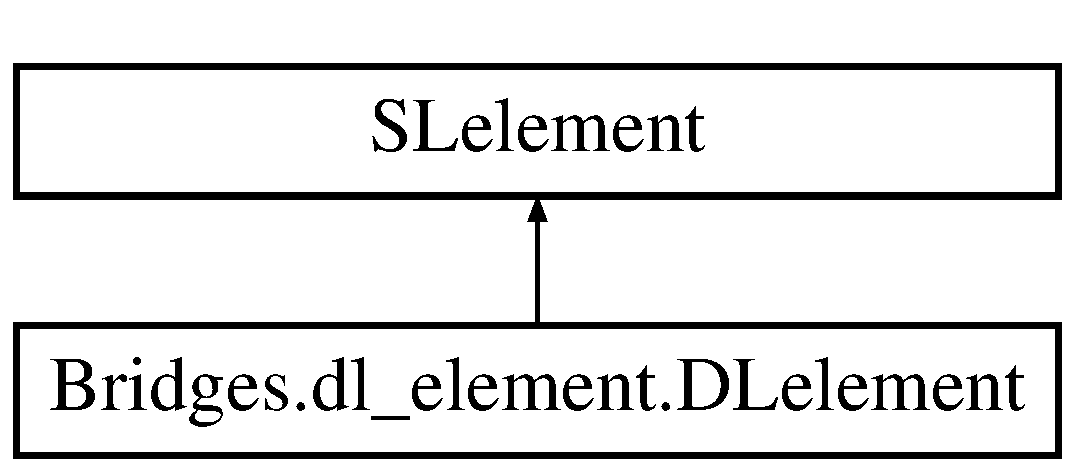
\includegraphics[height=2.000000cm]{class_bridges_1_1dl__element_1_1_d_lelement}
\end{center}
\end{figure}
\subsection*{Public Member Functions}
\begin{DoxyCompactItemize}
\item 
def \hyperlink{class_bridges_1_1dl__element_1_1_d_lelement_aeff7357e381b47df4ca8393b0ab58fd0}{\+\_\+\+\_\+init\+\_\+\+\_\+}
\begin{DoxyCompactList}\small\item\em Constructs an empty \hyperlink{class_bridges_1_1dl__element_1_1_d_lelement}{D\+Lelement}. \end{DoxyCompactList}\item 
def \hyperlink{class_bridges_1_1dl__element_1_1_d_lelement_a8e58440740696b00b0fbf466311a2e82}{get\+\_\+data\+\_\+structure\+\_\+type} (self)
\begin{DoxyCompactList}\small\item\em This method gets the data structure type. \end{DoxyCompactList}\item 
def \hyperlink{class_bridges_1_1dl__element_1_1_d_lelement_a494dbc772c5be2fedc1543c33ff18773}{get\+\_\+next} (self)
\begin{DoxyCompactList}\small\item\em This method returns the pointer to the next \hyperlink{class_bridges_1_1dl__element_1_1_d_lelement}{D\+Lelement}. \end{DoxyCompactList}\item 
def \hyperlink{class_bridges_1_1dl__element_1_1_d_lelement_ab3a51eae57870b6b45b09b8810d9b22b}{get\+\_\+prev} (self)
\begin{DoxyCompactList}\small\item\em This method sets the pointer to the next \hyperlink{class_bridges_1_1dl__element_1_1_d_lelement}{D\+Lelement}. \end{DoxyCompactList}\item 
def \hyperlink{class_bridges_1_1dl__element_1_1_d_lelement_a5a1281ba8e5d39551f6b0628b28cdda2}{set\+\_\+prev} (self, prv)
\begin{DoxyCompactList}\small\item\em This method sets the pointer to the previous \hyperlink{class_bridges_1_1dl__element_1_1_d_lelement}{D\+Lelement}. \end{DoxyCompactList}\item 
def \hyperlink{class_bridges_1_1dl__element_1_1_d_lelement_ab2019529a20633a852a06221b11776c9}{get\+\_\+data\+\_\+structure\+\_\+representation} (self)
\begin{DoxyCompactList}\small\item\em Get the J\+S\+O\+N representation of the the data structure. \end{DoxyCompactList}\end{DoxyCompactItemize}
\subsection*{Public Attributes}
\begin{DoxyCompactItemize}
\item 
\hyperlink{class_bridges_1_1dl__element_1_1_d_lelement_a5098c0244f6c4512db45f494266baf8a}{prev}
\end{DoxyCompactItemize}
\subsection*{Static Public Attributes}
\begin{DoxyCompactItemize}
\item 
tuple \hyperlink{class_bridges_1_1dl__element_1_1_d_lelement_a9f9abfb18c94eeac8d81a1ef6be5a398}{prev} = object()
\end{DoxyCompactItemize}


\subsection{Detailed Description}
This class is used to create doubly linked element objects. 

\begin{DoxyAuthor}{Author}
Mihai Mehedint, Kalpathi Subramanian
\end{DoxyAuthor}
\begin{DoxyVerb}This class extends Element and takes a generic parameter <E> representing
application specific data. This element forms the basic building block for
doubly linked lists. Doubly linked elements have two links,
"next" and "previous", that point to the previous and succeeding nodes along the list.

Elements contain a visualizer (ElementVisualizer) object for setting visual
attributes (color, shape, opacity, size), necessary for displaying them in a web
browser.

Elements also have a LinkVisualizer object that is used when they are linked to
another element, appropriate for setting link attributes, such as in linked lists,
between the current element and its next or previous nodes.\end{DoxyVerb}
 

\subsection{Constructor \& Destructor Documentation}
\hypertarget{class_bridges_1_1dl__element_1_1_d_lelement_aeff7357e381b47df4ca8393b0ab58fd0}{}\index{Bridges\+::dl\+\_\+element\+::\+D\+Lelement@{Bridges\+::dl\+\_\+element\+::\+D\+Lelement}!\+\_\+\+\_\+init\+\_\+\+\_\+@{\+\_\+\+\_\+init\+\_\+\+\_\+}}
\index{\+\_\+\+\_\+init\+\_\+\+\_\+@{\+\_\+\+\_\+init\+\_\+\+\_\+}!Bridges\+::dl\+\_\+element\+::\+D\+Lelement@{Bridges\+::dl\+\_\+element\+::\+D\+Lelement}}
\subsubsection[{\+\_\+\+\_\+init\+\_\+\+\_\+}]{\setlength{\rightskip}{0pt plus 5cm}def Bridges.\+dl\+\_\+element.\+D\+Lelement.\+\_\+\+\_\+init\+\_\+\+\_\+ (
\begin{DoxyParamCaption}
\item[{}]{self, }
\item[{}]{e = {\ttfamily None}, }
\item[{}]{label = {\ttfamily None}, }
\item[{}]{next = {\ttfamily None}, }
\item[{}]{prev = {\ttfamily None}}
\end{DoxyParamCaption}
)}\label{class_bridges_1_1dl__element_1_1_d_lelement_aeff7357e381b47df4ca8393b0ab58fd0}


Constructs an empty \hyperlink{class_bridges_1_1dl__element_1_1_d_lelement}{D\+Lelement}. 


\begin{DoxyParams}{Parameters}
{\em e} & the genereic object that this \hyperlink{class_bridges_1_1dl__element_1_1_d_lelement}{D\+Lelement} is holding \\
\hline
{\em next} & the \hyperlink{class_bridges_1_1dl__element_1_1_d_lelement}{D\+Lelement} that should be assigned to the next pointer \\
\hline
{\em prev} & the \hyperlink{class_bridges_1_1dl__element_1_1_d_lelement}{D\+Lelement} that should be assigned to the prev pointer \\
\hline
{\em label} & the label for this \hyperlink{class_bridges_1_1dl__element_1_1_d_lelement}{D\+Lelement} \\
\hline
\end{DoxyParams}


\subsection{Member Function Documentation}
\hypertarget{class_bridges_1_1dl__element_1_1_d_lelement_ab2019529a20633a852a06221b11776c9}{}\index{Bridges\+::dl\+\_\+element\+::\+D\+Lelement@{Bridges\+::dl\+\_\+element\+::\+D\+Lelement}!get\+\_\+data\+\_\+structure\+\_\+representation@{get\+\_\+data\+\_\+structure\+\_\+representation}}
\index{get\+\_\+data\+\_\+structure\+\_\+representation@{get\+\_\+data\+\_\+structure\+\_\+representation}!Bridges\+::dl\+\_\+element\+::\+D\+Lelement@{Bridges\+::dl\+\_\+element\+::\+D\+Lelement}}
\subsubsection[{get\+\_\+data\+\_\+structure\+\_\+representation(self)}]{\setlength{\rightskip}{0pt plus 5cm}def Bridges.\+dl\+\_\+element.\+D\+Lelement.\+get\+\_\+data\+\_\+structure\+\_\+representation (
\begin{DoxyParamCaption}
\item[{}]{self}
\end{DoxyParamCaption}
)}\label{class_bridges_1_1dl__element_1_1_d_lelement_ab2019529a20633a852a06221b11776c9}


Get the J\+S\+O\+N representation of the the data structure. 

\hypertarget{class_bridges_1_1dl__element_1_1_d_lelement_a8e58440740696b00b0fbf466311a2e82}{}\index{Bridges\+::dl\+\_\+element\+::\+D\+Lelement@{Bridges\+::dl\+\_\+element\+::\+D\+Lelement}!get\+\_\+data\+\_\+structure\+\_\+type@{get\+\_\+data\+\_\+structure\+\_\+type}}
\index{get\+\_\+data\+\_\+structure\+\_\+type@{get\+\_\+data\+\_\+structure\+\_\+type}!Bridges\+::dl\+\_\+element\+::\+D\+Lelement@{Bridges\+::dl\+\_\+element\+::\+D\+Lelement}}
\subsubsection[{get\+\_\+data\+\_\+structure\+\_\+type(self)}]{\setlength{\rightskip}{0pt plus 5cm}def Bridges.\+dl\+\_\+element.\+D\+Lelement.\+get\+\_\+data\+\_\+structure\+\_\+type (
\begin{DoxyParamCaption}
\item[{}]{self}
\end{DoxyParamCaption}
)}\label{class_bridges_1_1dl__element_1_1_d_lelement_a8e58440740696b00b0fbf466311a2e82}


This method gets the data structure type. 

\begin{DoxyReturn}{Returns}
The date structure type as a string 
\end{DoxyReturn}
\hypertarget{class_bridges_1_1dl__element_1_1_d_lelement_a494dbc772c5be2fedc1543c33ff18773}{}\index{Bridges\+::dl\+\_\+element\+::\+D\+Lelement@{Bridges\+::dl\+\_\+element\+::\+D\+Lelement}!get\+\_\+next@{get\+\_\+next}}
\index{get\+\_\+next@{get\+\_\+next}!Bridges\+::dl\+\_\+element\+::\+D\+Lelement@{Bridges\+::dl\+\_\+element\+::\+D\+Lelement}}
\subsubsection[{get\+\_\+next(self)}]{\setlength{\rightskip}{0pt plus 5cm}def Bridges.\+dl\+\_\+element.\+D\+Lelement.\+get\+\_\+next (
\begin{DoxyParamCaption}
\item[{}]{self}
\end{DoxyParamCaption}
)}\label{class_bridges_1_1dl__element_1_1_d_lelement_a494dbc772c5be2fedc1543c33ff18773}


This method returns the pointer to the next \hyperlink{class_bridges_1_1dl__element_1_1_d_lelement}{D\+Lelement}. 

\begin{DoxyReturn}{Returns}
the \hyperlink{class_bridges_1_1dl__element_1_1_d_lelement}{D\+Lelement} assigned to the next pointer 
\end{DoxyReturn}
\hypertarget{class_bridges_1_1dl__element_1_1_d_lelement_ab3a51eae57870b6b45b09b8810d9b22b}{}\index{Bridges\+::dl\+\_\+element\+::\+D\+Lelement@{Bridges\+::dl\+\_\+element\+::\+D\+Lelement}!get\+\_\+prev@{get\+\_\+prev}}
\index{get\+\_\+prev@{get\+\_\+prev}!Bridges\+::dl\+\_\+element\+::\+D\+Lelement@{Bridges\+::dl\+\_\+element\+::\+D\+Lelement}}
\subsubsection[{get\+\_\+prev(self)}]{\setlength{\rightskip}{0pt plus 5cm}def Bridges.\+dl\+\_\+element.\+D\+Lelement.\+get\+\_\+prev (
\begin{DoxyParamCaption}
\item[{}]{self}
\end{DoxyParamCaption}
)}\label{class_bridges_1_1dl__element_1_1_d_lelement_ab3a51eae57870b6b45b09b8810d9b22b}


This method sets the pointer to the next \hyperlink{class_bridges_1_1dl__element_1_1_d_lelement}{D\+Lelement}. 


\begin{DoxyParams}{Parameters}
{\em next} & the \hyperlink{class_bridges_1_1dl__element_1_1_d_lelement}{D\+Lelement} that should be assigned to the next pointer\\
\hline
\end{DoxyParams}
\begin{DoxyVerb}    public void setNext(DLelement<E> nxt) {
        this.next = nxt;
        if (nxt != null)
            this.setLinkVisualizer(nxt);
    }
\end{DoxyVerb}


This method returns the pointer to the previous \hyperlink{class_bridges_1_1dl__element_1_1_d_lelement}{D\+Lelement}

\begin{DoxyReturn}{Returns}
the \hyperlink{class_bridges_1_1dl__element_1_1_d_lelement}{D\+Lelement} assigned to the prev pointer 
\end{DoxyReturn}
\hypertarget{class_bridges_1_1dl__element_1_1_d_lelement_a5a1281ba8e5d39551f6b0628b28cdda2}{}\index{Bridges\+::dl\+\_\+element\+::\+D\+Lelement@{Bridges\+::dl\+\_\+element\+::\+D\+Lelement}!set\+\_\+prev@{set\+\_\+prev}}
\index{set\+\_\+prev@{set\+\_\+prev}!Bridges\+::dl\+\_\+element\+::\+D\+Lelement@{Bridges\+::dl\+\_\+element\+::\+D\+Lelement}}
\subsubsection[{set\+\_\+prev(self, prv)}]{\setlength{\rightskip}{0pt plus 5cm}def Bridges.\+dl\+\_\+element.\+D\+Lelement.\+set\+\_\+prev (
\begin{DoxyParamCaption}
\item[{}]{self, }
\item[{}]{prv}
\end{DoxyParamCaption}
)}\label{class_bridges_1_1dl__element_1_1_d_lelement_a5a1281ba8e5d39551f6b0628b28cdda2}


This method sets the pointer to the previous \hyperlink{class_bridges_1_1dl__element_1_1_d_lelement}{D\+Lelement}. 


\begin{DoxyParams}{Parameters}
{\em prev} & the \hyperlink{class_bridges_1_1dl__element_1_1_d_lelement}{D\+Lelement} that should be assigned to the prev pointer \\
\hline
\end{DoxyParams}


\subsection{Member Data Documentation}
\hypertarget{class_bridges_1_1dl__element_1_1_d_lelement_a9f9abfb18c94eeac8d81a1ef6be5a398}{}\index{Bridges\+::dl\+\_\+element\+::\+D\+Lelement@{Bridges\+::dl\+\_\+element\+::\+D\+Lelement}!prev@{prev}}
\index{prev@{prev}!Bridges\+::dl\+\_\+element\+::\+D\+Lelement@{Bridges\+::dl\+\_\+element\+::\+D\+Lelement}}
\subsubsection[{prev}]{\setlength{\rightskip}{0pt plus 5cm}tuple Bridges.\+dl\+\_\+element.\+D\+Lelement.\+prev = object()\hspace{0.3cm}{\ttfamily [static]}}\label{class_bridges_1_1dl__element_1_1_d_lelement_a9f9abfb18c94eeac8d81a1ef6be5a398}
\hypertarget{class_bridges_1_1dl__element_1_1_d_lelement_a5098c0244f6c4512db45f494266baf8a}{}\index{Bridges\+::dl\+\_\+element\+::\+D\+Lelement@{Bridges\+::dl\+\_\+element\+::\+D\+Lelement}!prev@{prev}}
\index{prev@{prev}!Bridges\+::dl\+\_\+element\+::\+D\+Lelement@{Bridges\+::dl\+\_\+element\+::\+D\+Lelement}}
\subsubsection[{prev}]{\setlength{\rightskip}{0pt plus 5cm}Bridges.\+dl\+\_\+element.\+D\+Lelement.\+prev}\label{class_bridges_1_1dl__element_1_1_d_lelement_a5098c0244f6c4512db45f494266baf8a}


The documentation for this class was generated from the following file\+:\begin{DoxyCompactItemize}
\item 
/\+Users/kalpathi/gr/bridges/client/python/\+Bridges/\hyperlink{dl__element_8py}{dl\+\_\+element.\+py}\end{DoxyCompactItemize}

\hypertarget{class_bridges_1_1edge_1_1_edge}{}\section{Bridges.\+edge.\+Edge Class Reference}
\label{class_bridges_1_1edge_1_1_edge}\index{Bridges.\+edge.\+Edge@{Bridges.\+edge.\+Edge}}


This class is used to represent the edges in a graph and will appear as links in the B\+R\+I\+D\+G\+E\+S graph visualization.  


Inheritance diagram for Bridges.\+edge.\+Edge\+:\begin{figure}[H]
\begin{center}
\leavevmode
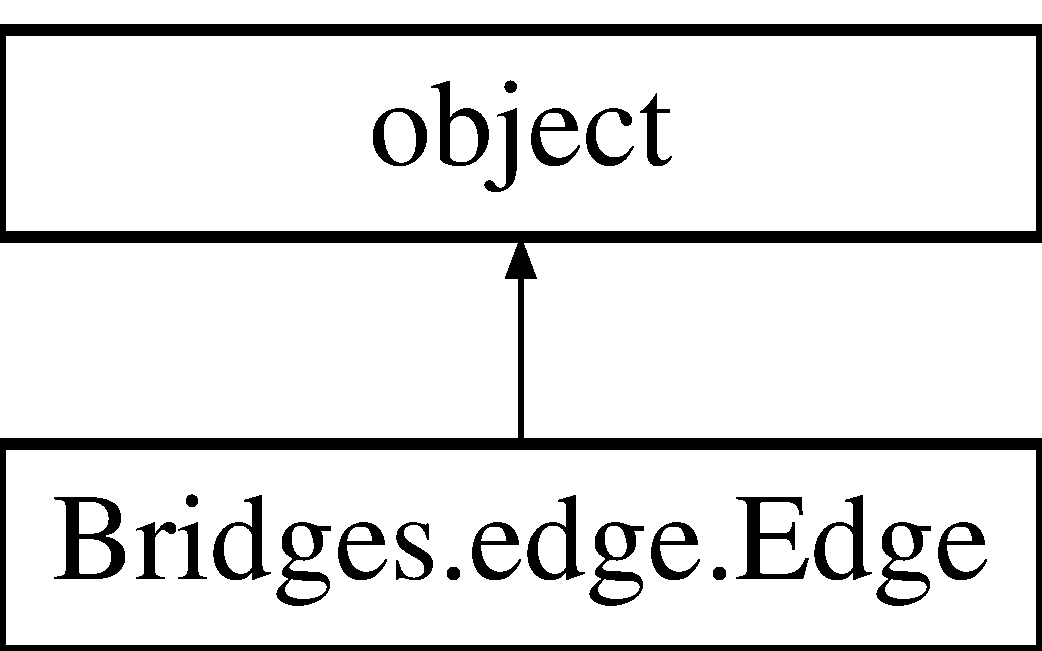
\includegraphics[height=2.000000cm]{class_bridges_1_1edge_1_1_edge}
\end{center}
\end{figure}
\subsection*{Public Member Functions}
\begin{DoxyCompactItemize}
\item 
def \hyperlink{class_bridges_1_1edge_1_1_edge_a5e55af43202cf2d6a0e433481d422788}{\+\_\+\+\_\+init\+\_\+\+\_\+}
\begin{DoxyCompactList}\small\item\em Constructors. \end{DoxyCompactList}\item 
def \hyperlink{class_bridges_1_1edge_1_1_edge_a6e6cd15ddf1a1550edbdcc947b8bf52c}{set\+\_\+weight} (self, wt)
\begin{DoxyCompactList}\small\item\em Set edge weight to \char`\"{}wt\char`\"{}. \end{DoxyCompactList}\item 
def \hyperlink{class_bridges_1_1edge_1_1_edge_a014aeea3de184a001bc0dec8c4c76189}{get\+\_\+weight} (self)
\begin{DoxyCompactList}\small\item\em Get edge weight. \end{DoxyCompactList}\item 
def \hyperlink{class_bridges_1_1edge_1_1_edge_a8d8d9c805341d0d6dd45210d740d7de1}{set\+\_\+vertex} (self, v)
\begin{DoxyCompactList}\small\item\em Set terminating Element of the edge. \end{DoxyCompactList}\item 
def \hyperlink{class_bridges_1_1edge_1_1_edge_a68e890b1ad5a01ef69bee809b7b526d1}{get\+\_\+vertex} (self)
\begin{DoxyCompactList}\small\item\em Get identifer of the terminating Element of edge. \end{DoxyCompactList}\item 
def \hyperlink{class_bridges_1_1edge_1_1_edge_aa65288b314e414374bc3d2e0a0792c03}{set\+\_\+edge} (self, wt, v)
\begin{DoxyCompactList}\small\item\em Set edge to weight of \char`\"{}wt\char`\"{} and terminating Elememt of \char`\"{}v\char`\"{}. \end{DoxyCompactList}\item 
def \hyperlink{class_bridges_1_1edge_1_1_edge_aa9ca872601b29ed48d492c7a54a1cc42}{set\+\_\+edge\+\_\+data} (self, data)
\begin{DoxyCompactList}\small\item\em Set \hyperlink{class_bridges_1_1edge_1_1_edge}{Edge} data (represented as a string for now) \end{DoxyCompactList}\item 
def \hyperlink{class_bridges_1_1edge_1_1_edge_a37f3fa415dc037ee5ef32aafc3c24792}{get\+\_\+edge\+\_\+data} (self)
\begin{DoxyCompactList}\small\item\em Get edge data. \end{DoxyCompactList}\item 
def \hyperlink{class_bridges_1_1edge_1_1_edge_a00fbdf3e8b0e05e00647cd2a32b25beb}{get\+\_\+edge} (self)
\begin{DoxyCompactList}\small\item\em Returns this edge. \end{DoxyCompactList}\end{DoxyCompactItemize}
\subsection*{Public Attributes}
\begin{DoxyCompactItemize}
\item 
\hyperlink{class_bridges_1_1edge_1_1_edge_a36787799fbbb1cd17fe1944d92513524}{weight}
\item 
\hyperlink{class_bridges_1_1edge_1_1_edge_a785d6e63ec4a7ec1b49c9e4a81a802dc}{vertex}
\item 
\hyperlink{class_bridges_1_1edge_1_1_edge_a7677bdbf69f6a1725be3bb79e2bb1c7e}{edge\+\_\+data}
\end{DoxyCompactItemize}
\subsection*{Static Public Attributes}
\begin{DoxyCompactItemize}
\item 
tuple \hyperlink{class_bridges_1_1edge_1_1_edge_a4fb568704945fe2cc8fbb1f5c5e807cd}{weight} = int()
\item 
tuple \hyperlink{class_bridges_1_1edge_1_1_edge_a1cded0b08960b1a7fa0d8c1505315651}{vertex} = Element()
\item 
tuple \hyperlink{class_bridges_1_1edge_1_1_edge_a982756166f2c8c6321a060cc377f2c04}{edge\+\_\+data} = str()
\end{DoxyCompactItemize}


\subsection{Detailed Description}
This class is used to represent the edges in a graph and will appear as links in the B\+R\+I\+D\+G\+E\+S graph visualization. 

This object is used in graphs and graph algorithms such as D\+F\+S, B\+F\+S and shortest path algorithms that need to visit graph edges. The adjacency list representation uses them as the generic paramter, as S\+Lelement$<$\+Edge$>$ bridges represents Edges as links between pairs of elements

\begin{DoxyAuthor}{Author}
K.\+R. Subramanian 
\end{DoxyAuthor}


\subsection{Constructor \& Destructor Documentation}
\hypertarget{class_bridges_1_1edge_1_1_edge_a5e55af43202cf2d6a0e433481d422788}{}\index{Bridges\+::edge\+::\+Edge@{Bridges\+::edge\+::\+Edge}!\+\_\+\+\_\+init\+\_\+\+\_\+@{\+\_\+\+\_\+init\+\_\+\+\_\+}}
\index{\+\_\+\+\_\+init\+\_\+\+\_\+@{\+\_\+\+\_\+init\+\_\+\+\_\+}!Bridges\+::edge\+::\+Edge@{Bridges\+::edge\+::\+Edge}}
\subsubsection[{\+\_\+\+\_\+init\+\_\+\+\_\+}]{\setlength{\rightskip}{0pt plus 5cm}def Bridges.\+edge.\+Edge.\+\_\+\+\_\+init\+\_\+\+\_\+ (
\begin{DoxyParamCaption}
\item[{}]{self, }
\item[{}]{wt = {\ttfamily None}, }
\item[{}]{v = {\ttfamily None}}
\end{DoxyParamCaption}
)}\label{class_bridges_1_1edge_1_1_edge_a5e55af43202cf2d6a0e433481d422788}


Constructors. 


\begin{DoxyParams}{Parameters}
{\em wt} & integer, representing edge weight \\
\hline
{\em v} & the terminating vertex of the edge \\
\hline
\end{DoxyParams}


\subsection{Member Function Documentation}
\hypertarget{class_bridges_1_1edge_1_1_edge_a00fbdf3e8b0e05e00647cd2a32b25beb}{}\index{Bridges\+::edge\+::\+Edge@{Bridges\+::edge\+::\+Edge}!get\+\_\+edge@{get\+\_\+edge}}
\index{get\+\_\+edge@{get\+\_\+edge}!Bridges\+::edge\+::\+Edge@{Bridges\+::edge\+::\+Edge}}
\subsubsection[{get\+\_\+edge(self)}]{\setlength{\rightskip}{0pt plus 5cm}def Bridges.\+edge.\+Edge.\+get\+\_\+edge (
\begin{DoxyParamCaption}
\item[{}]{self}
\end{DoxyParamCaption}
)}\label{class_bridges_1_1edge_1_1_edge_a00fbdf3e8b0e05e00647cd2a32b25beb}


Returns this edge. 

\hypertarget{class_bridges_1_1edge_1_1_edge_a37f3fa415dc037ee5ef32aafc3c24792}{}\index{Bridges\+::edge\+::\+Edge@{Bridges\+::edge\+::\+Edge}!get\+\_\+edge\+\_\+data@{get\+\_\+edge\+\_\+data}}
\index{get\+\_\+edge\+\_\+data@{get\+\_\+edge\+\_\+data}!Bridges\+::edge\+::\+Edge@{Bridges\+::edge\+::\+Edge}}
\subsubsection[{get\+\_\+edge\+\_\+data(self)}]{\setlength{\rightskip}{0pt plus 5cm}def Bridges.\+edge.\+Edge.\+get\+\_\+edge\+\_\+data (
\begin{DoxyParamCaption}
\item[{}]{self}
\end{DoxyParamCaption}
)}\label{class_bridges_1_1edge_1_1_edge_a37f3fa415dc037ee5ef32aafc3c24792}


Get edge data. 

\begin{DoxyReturn}{Returns}
the edge data 
\end{DoxyReturn}
\hypertarget{class_bridges_1_1edge_1_1_edge_a68e890b1ad5a01ef69bee809b7b526d1}{}\index{Bridges\+::edge\+::\+Edge@{Bridges\+::edge\+::\+Edge}!get\+\_\+vertex@{get\+\_\+vertex}}
\index{get\+\_\+vertex@{get\+\_\+vertex}!Bridges\+::edge\+::\+Edge@{Bridges\+::edge\+::\+Edge}}
\subsubsection[{get\+\_\+vertex(self)}]{\setlength{\rightskip}{0pt plus 5cm}def Bridges.\+edge.\+Edge.\+get\+\_\+vertex (
\begin{DoxyParamCaption}
\item[{}]{self}
\end{DoxyParamCaption}
)}\label{class_bridges_1_1edge_1_1_edge_a68e890b1ad5a01ef69bee809b7b526d1}


Get identifer of the terminating Element of edge. 

\begin{DoxyReturn}{Returns}
the string identifier of the terminating Element 
\end{DoxyReturn}
\hypertarget{class_bridges_1_1edge_1_1_edge_a014aeea3de184a001bc0dec8c4c76189}{}\index{Bridges\+::edge\+::\+Edge@{Bridges\+::edge\+::\+Edge}!get\+\_\+weight@{get\+\_\+weight}}
\index{get\+\_\+weight@{get\+\_\+weight}!Bridges\+::edge\+::\+Edge@{Bridges\+::edge\+::\+Edge}}
\subsubsection[{get\+\_\+weight(self)}]{\setlength{\rightskip}{0pt plus 5cm}def Bridges.\+edge.\+Edge.\+get\+\_\+weight (
\begin{DoxyParamCaption}
\item[{}]{self}
\end{DoxyParamCaption}
)}\label{class_bridges_1_1edge_1_1_edge_a014aeea3de184a001bc0dec8c4c76189}


Get edge weight. 

\begin{DoxyReturn}{Returns}
the weight of edge 
\end{DoxyReturn}
\hypertarget{class_bridges_1_1edge_1_1_edge_aa65288b314e414374bc3d2e0a0792c03}{}\index{Bridges\+::edge\+::\+Edge@{Bridges\+::edge\+::\+Edge}!set\+\_\+edge@{set\+\_\+edge}}
\index{set\+\_\+edge@{set\+\_\+edge}!Bridges\+::edge\+::\+Edge@{Bridges\+::edge\+::\+Edge}}
\subsubsection[{set\+\_\+edge(self, wt, v)}]{\setlength{\rightskip}{0pt plus 5cm}def Bridges.\+edge.\+Edge.\+set\+\_\+edge (
\begin{DoxyParamCaption}
\item[{}]{self, }
\item[{}]{wt, }
\item[{}]{v}
\end{DoxyParamCaption}
)}\label{class_bridges_1_1edge_1_1_edge_aa65288b314e414374bc3d2e0a0792c03}


Set edge to weight of \char`\"{}wt\char`\"{} and terminating Elememt of \char`\"{}v\char`\"{}. 


\begin{DoxyParams}{Parameters}
{\em wt} & edge weight \\
\hline
{\em v} & the identifier of the terminating Element \\
\hline
\end{DoxyParams}
\hypertarget{class_bridges_1_1edge_1_1_edge_aa9ca872601b29ed48d492c7a54a1cc42}{}\index{Bridges\+::edge\+::\+Edge@{Bridges\+::edge\+::\+Edge}!set\+\_\+edge\+\_\+data@{set\+\_\+edge\+\_\+data}}
\index{set\+\_\+edge\+\_\+data@{set\+\_\+edge\+\_\+data}!Bridges\+::edge\+::\+Edge@{Bridges\+::edge\+::\+Edge}}
\subsubsection[{set\+\_\+edge\+\_\+data(self, data)}]{\setlength{\rightskip}{0pt plus 5cm}def Bridges.\+edge.\+Edge.\+set\+\_\+edge\+\_\+data (
\begin{DoxyParamCaption}
\item[{}]{self, }
\item[{}]{data}
\end{DoxyParamCaption}
)}\label{class_bridges_1_1edge_1_1_edge_aa9ca872601b29ed48d492c7a54a1cc42}


Set \hyperlink{class_bridges_1_1edge_1_1_edge}{Edge} data (represented as a string for now) 


\begin{DoxyParams}{Parameters}
{\em string} & application data \\
\hline
\end{DoxyParams}
\hypertarget{class_bridges_1_1edge_1_1_edge_a8d8d9c805341d0d6dd45210d740d7de1}{}\index{Bridges\+::edge\+::\+Edge@{Bridges\+::edge\+::\+Edge}!set\+\_\+vertex@{set\+\_\+vertex}}
\index{set\+\_\+vertex@{set\+\_\+vertex}!Bridges\+::edge\+::\+Edge@{Bridges\+::edge\+::\+Edge}}
\subsubsection[{set\+\_\+vertex(self, v)}]{\setlength{\rightskip}{0pt plus 5cm}def Bridges.\+edge.\+Edge.\+set\+\_\+vertex (
\begin{DoxyParamCaption}
\item[{}]{self, }
\item[{}]{v}
\end{DoxyParamCaption}
)}\label{class_bridges_1_1edge_1_1_edge_a8d8d9c805341d0d6dd45210d740d7de1}


Set terminating Element of the edge. 


\begin{DoxyParams}{Parameters}
{\em v} & the identifier of the terminating Element \\
\hline
\end{DoxyParams}
\hypertarget{class_bridges_1_1edge_1_1_edge_a6e6cd15ddf1a1550edbdcc947b8bf52c}{}\index{Bridges\+::edge\+::\+Edge@{Bridges\+::edge\+::\+Edge}!set\+\_\+weight@{set\+\_\+weight}}
\index{set\+\_\+weight@{set\+\_\+weight}!Bridges\+::edge\+::\+Edge@{Bridges\+::edge\+::\+Edge}}
\subsubsection[{set\+\_\+weight(self, wt)}]{\setlength{\rightskip}{0pt plus 5cm}def Bridges.\+edge.\+Edge.\+set\+\_\+weight (
\begin{DoxyParamCaption}
\item[{}]{self, }
\item[{}]{wt}
\end{DoxyParamCaption}
)}\label{class_bridges_1_1edge_1_1_edge_a6e6cd15ddf1a1550edbdcc947b8bf52c}


Set edge weight to \char`\"{}wt\char`\"{}. 


\begin{DoxyParams}{Parameters}
{\em wt} & -\/ graph edge weight \\
\hline
\end{DoxyParams}


\subsection{Member Data Documentation}
\hypertarget{class_bridges_1_1edge_1_1_edge_a982756166f2c8c6321a060cc377f2c04}{}\index{Bridges\+::edge\+::\+Edge@{Bridges\+::edge\+::\+Edge}!edge\+\_\+data@{edge\+\_\+data}}
\index{edge\+\_\+data@{edge\+\_\+data}!Bridges\+::edge\+::\+Edge@{Bridges\+::edge\+::\+Edge}}
\subsubsection[{edge\+\_\+data}]{\setlength{\rightskip}{0pt plus 5cm}tuple Bridges.\+edge.\+Edge.\+edge\+\_\+data = str()\hspace{0.3cm}{\ttfamily [static]}}\label{class_bridges_1_1edge_1_1_edge_a982756166f2c8c6321a060cc377f2c04}
\hypertarget{class_bridges_1_1edge_1_1_edge_a7677bdbf69f6a1725be3bb79e2bb1c7e}{}\index{Bridges\+::edge\+::\+Edge@{Bridges\+::edge\+::\+Edge}!edge\+\_\+data@{edge\+\_\+data}}
\index{edge\+\_\+data@{edge\+\_\+data}!Bridges\+::edge\+::\+Edge@{Bridges\+::edge\+::\+Edge}}
\subsubsection[{edge\+\_\+data}]{\setlength{\rightskip}{0pt plus 5cm}Bridges.\+edge.\+Edge.\+edge\+\_\+data}\label{class_bridges_1_1edge_1_1_edge_a7677bdbf69f6a1725be3bb79e2bb1c7e}
\hypertarget{class_bridges_1_1edge_1_1_edge_a1cded0b08960b1a7fa0d8c1505315651}{}\index{Bridges\+::edge\+::\+Edge@{Bridges\+::edge\+::\+Edge}!vertex@{vertex}}
\index{vertex@{vertex}!Bridges\+::edge\+::\+Edge@{Bridges\+::edge\+::\+Edge}}
\subsubsection[{vertex}]{\setlength{\rightskip}{0pt plus 5cm}tuple Bridges.\+edge.\+Edge.\+vertex = Element()\hspace{0.3cm}{\ttfamily [static]}}\label{class_bridges_1_1edge_1_1_edge_a1cded0b08960b1a7fa0d8c1505315651}
\hypertarget{class_bridges_1_1edge_1_1_edge_a785d6e63ec4a7ec1b49c9e4a81a802dc}{}\index{Bridges\+::edge\+::\+Edge@{Bridges\+::edge\+::\+Edge}!vertex@{vertex}}
\index{vertex@{vertex}!Bridges\+::edge\+::\+Edge@{Bridges\+::edge\+::\+Edge}}
\subsubsection[{vertex}]{\setlength{\rightskip}{0pt plus 5cm}Bridges.\+edge.\+Edge.\+vertex}\label{class_bridges_1_1edge_1_1_edge_a785d6e63ec4a7ec1b49c9e4a81a802dc}
\hypertarget{class_bridges_1_1edge_1_1_edge_a4fb568704945fe2cc8fbb1f5c5e807cd}{}\index{Bridges\+::edge\+::\+Edge@{Bridges\+::edge\+::\+Edge}!weight@{weight}}
\index{weight@{weight}!Bridges\+::edge\+::\+Edge@{Bridges\+::edge\+::\+Edge}}
\subsubsection[{weight}]{\setlength{\rightskip}{0pt plus 5cm}tuple Bridges.\+edge.\+Edge.\+weight = int()\hspace{0.3cm}{\ttfamily [static]}}\label{class_bridges_1_1edge_1_1_edge_a4fb568704945fe2cc8fbb1f5c5e807cd}
\hypertarget{class_bridges_1_1edge_1_1_edge_a36787799fbbb1cd17fe1944d92513524}{}\index{Bridges\+::edge\+::\+Edge@{Bridges\+::edge\+::\+Edge}!weight@{weight}}
\index{weight@{weight}!Bridges\+::edge\+::\+Edge@{Bridges\+::edge\+::\+Edge}}
\subsubsection[{weight}]{\setlength{\rightskip}{0pt plus 5cm}Bridges.\+edge.\+Edge.\+weight}\label{class_bridges_1_1edge_1_1_edge_a36787799fbbb1cd17fe1944d92513524}


The documentation for this class was generated from the following file\+:\begin{DoxyCompactItemize}
\item 
/\+Users/kalpathi/gr/bridges/client/python/\+Bridges/\hyperlink{edge_8py}{edge.\+py}\end{DoxyCompactItemize}

\hypertarget{class_bridges_1_1element_1_1_element}{}\section{Bridges.\+element.\+Element Class Reference}
\label{class_bridges_1_1element_1_1_element}\index{Bridges.\+element.\+Element@{Bridges.\+element.\+Element}}


This is the main superclass in B\+R\+I\+D\+G\+E\+S for deriving a number of objects used in building arrays, lists, trees and graph data structures.  


Inheritance diagram for Bridges.\+element.\+Element\+:\begin{figure}[H]
\begin{center}
\leavevmode
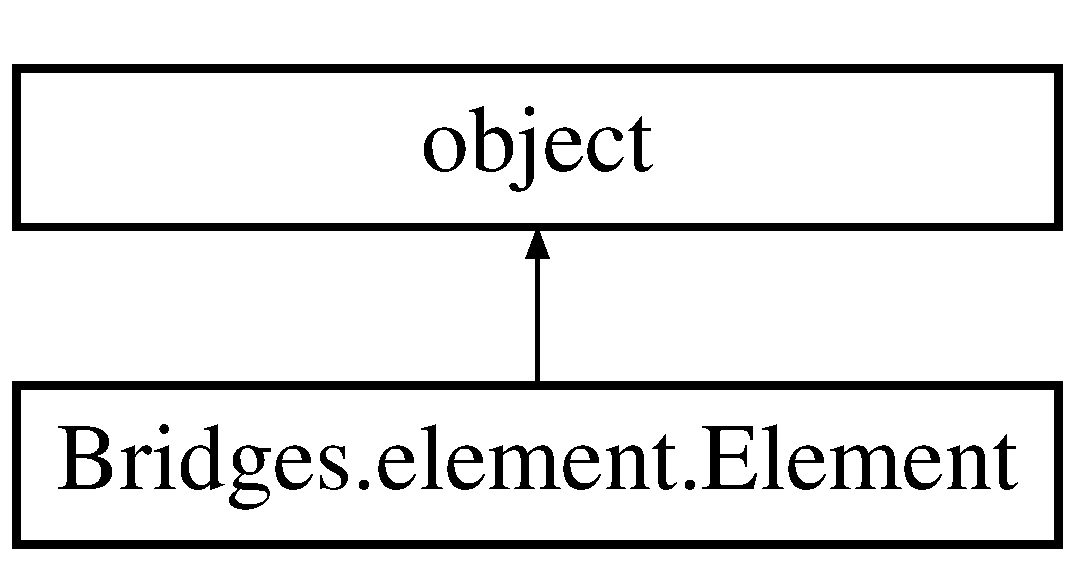
\includegraphics[height=2.000000cm]{class_bridges_1_1element_1_1_element}
\end{center}
\end{figure}
\subsection*{Public Member Functions}
\begin{DoxyCompactItemize}
\item 
def \hyperlink{class_bridges_1_1element_1_1_element_aeb25959809a6c89fa7a1fcb55378e751}{get\+\_\+data\+\_\+struct\+\_\+type} (self)
\item 
def \hyperlink{class_bridges_1_1element_1_1_element_a85f37d5c7a6e8f45c200a5ee7c42eb6e}{\+\_\+\+\_\+init\+\_\+\+\_\+}
\begin{DoxyCompactList}\small\item\em \hyperlink{class_bridges_1_1element_1_1_element}{Element} constructor creates an Element\+Visualizer object sets a unique identifier for the current \hyperlink{class_bridges_1_1element_1_1_element}{Element} normally used from subclasses. \end{DoxyCompactList}\item 
def \hyperlink{class_bridges_1_1element_1_1_element_a01b3d0e57ce06b996629acdb1cfaafb6}{get\+\_\+identifier} (self)
\begin{DoxyCompactList}\small\item\em this method returns the element\textquotesingle{}s unique identifier \end{DoxyCompactList}\item 
def \hyperlink{class_bridges_1_1element_1_1_element_a0f9c10a5424253aa27f2737e9d1c5411}{get\+\_\+visualizer} (self)
\begin{DoxyCompactList}\small\item\em Returns the \hyperlink{class_bridges_1_1element_1_1_element}{Element}\textquotesingle{}s visualizer object. \end{DoxyCompactList}\item 
def \hyperlink{class_bridges_1_1element_1_1_element_a8147ac170339450e4c375fd66dd2f863}{set\+\_\+visualizer} (self, \hyperlink{class_bridges_1_1element_1_1_element_a929f63e3aaaeff971a1def438168559a}{visualizer})
\begin{DoxyCompactList}\small\item\em This method sets the visualizer object for the current element object. \end{DoxyCompactList}\item 
def \hyperlink{class_bridges_1_1element_1_1_element_af79b3fc0a157602a476b672e6ecd9dcb}{get\+\_\+link\+\_\+visualizer} (self, el)
\begin{DoxyCompactList}\small\item\em Returns the \hyperlink{class_bridges_1_1element_1_1_element}{Element}\textquotesingle{}s link visualizer object. \end{DoxyCompactList}\item 
def \hyperlink{class_bridges_1_1element_1_1_element_a6ae09d81f76766ab3de9e48f01c5d509}{set\+\_\+link\+\_\+visualizer} (self, el)
\begin{DoxyCompactList}\small\item\em Sets the link from this element to a new incoming element. \end{DoxyCompactList}\item 
def \hyperlink{class_bridges_1_1element_1_1_element_a6e5f677881cc9837963c7d1082a6e079}{remove\+\_\+link\+\_\+visualizer} (self, el)
\item 
def \hyperlink{class_bridges_1_1element_1_1_element_ade4aee8d863fcb0233d1f1f659b1c0a6}{get\+\_\+class\+\_\+name} (self)
\begin{DoxyCompactList}\small\item\em Validates the \hyperlink{class_bridges_1_1element_1_1_element}{Element}\textquotesingle{}s value when the \hyperlink{class_bridges_1_1element_1_1_element}{Element} is created A non null value is expected this will be unnecessary after we modify the server. \end{DoxyCompactList}\item 
def \hyperlink{class_bridges_1_1element_1_1_element_af40cae0b8b917516c86936d3d0d16f3b}{get\+\_\+element\+\_\+representation} (self)
\item 
def \hyperlink{class_bridges_1_1element_1_1_element_a3ec5ef88f83374296a873fed8f0f1806}{get\+\_\+link\+\_\+representation} (self, lv, src, dest)
\item 
def \hyperlink{class_bridges_1_1element_1_1_element_a8705da5768e08fdcd5a73979c7e47c80}{get\+\_\+label} (self)
\begin{DoxyCompactList}\small\item\em This method returns the existing value of the label fields. \end{DoxyCompactList}\item 
def \hyperlink{class_bridges_1_1element_1_1_element_a87e7664cd328b32bd978b241d8f8ad88}{set\+\_\+label} (self, \hyperlink{class_bridges_1_1element_1_1_element_ad5a528474853ed245d14e7d4db015294}{label})
\begin{DoxyCompactList}\small\item\em This method sets the label. \end{DoxyCompactList}\item 
def \hyperlink{class_bridges_1_1element_1_1_element_a17f4120ec937cee6779aaa9f2139d3a7}{arrange\+\_\+label} (self, \hyperlink{class_bridges_1_1element_1_1_element_ad5a528474853ed245d14e7d4db015294}{label}, \hyperlink{class_bridges_1_1element_1_1_element_a63a7f47da997db2df55a22715e519dff}{word\+\_\+number})
\begin{DoxyCompactList}\small\item\em This method formats the label string using a predefine pattern (D\+I\+V\+I\+D\+E\+\_\+\+K\+E\+Y) and replaces the pattern with the string characters hold by the I\+N\+S\+E\+R\+T\+\_\+\+S\+T\+R\+I\+N\+G global variable. \end{DoxyCompactList}\item 
def \hyperlink{class_bridges_1_1element_1_1_element_a823d51c9beb771d1e8286160ae6b7db3}{get\+\_\+value} (self)
\begin{DoxyCompactList}\small\item\em This method returns the generic parameter value held in the element. \end{DoxyCompactList}\item 
def \hyperlink{class_bridges_1_1element_1_1_element_a83180a28821ad37ed8df1f28267df1cf}{set\+\_\+value} (self, \hyperlink{class_bridges_1_1element_1_1_element_af18dea5cfca666c8e4ae29f1a464e7ea}{value})
\begin{DoxyCompactList}\small\item\em This method sets the generic parameter value for this element. \end{DoxyCompactList}\item 
def \hyperlink{class_bridges_1_1element_1_1_element_affacf899ae3b7215323848cde7583a2c}{\+\_\+\+\_\+str\+\_\+\+\_\+} (self)
\end{DoxyCompactItemize}
\subsection*{Public Attributes}
\begin{DoxyCompactItemize}
\item 
\hyperlink{class_bridges_1_1element_1_1_element_a929f63e3aaaeff971a1def438168559a}{visualizer}
\item 
\hyperlink{class_bridges_1_1element_1_1_element_a41950f899961e5eebd871ede8244792e}{lvisualizer}
\item 
\hyperlink{class_bridges_1_1element_1_1_element_a508cace0ae2f124b1933c1304fb063cf}{identifier}
\item 
\hyperlink{class_bridges_1_1element_1_1_element_a0aedaa53836e4af0c2d81a0a5b16115a}{label}
\item 
\hyperlink{class_bridges_1_1element_1_1_element_a8fdf33053fd2e19e47f7b96d4641ecc6}{ids}
\item 
\hyperlink{class_bridges_1_1element_1_1_element_a54928aa5d8a914e9394ba2fb0e7ef270}{value}
\end{DoxyCompactItemize}
\subsection*{Static Public Attributes}
\begin{DoxyCompactItemize}
\item 
string \hyperlink{class_bridges_1_1element_1_1_element_adedb8dd49c1cdb5f53ec0d7199e397d8}{Q\+U\+O\+T\+E} = \char`\"{}\textbackslash{}\char`\"{}\char`\"{}
\item 
string \hyperlink{class_bridges_1_1element_1_1_element_ac1a168f60bd05dc9306e780b7632f747}{C\+O\+M\+M\+A} = \char`\"{},\char`\"{}
\item 
string \hyperlink{class_bridges_1_1element_1_1_element_a7dd3794d50d185656457deb8cb5dbe04}{C\+O\+L\+O\+N} = \char`\"{}\+:\char`\"{}
\item 
string \hyperlink{class_bridges_1_1element_1_1_element_a437f27e93bcfe39a510a7c0916dfce34}{O\+P\+E\+N\+\_\+\+C\+U\+R\+L\+Y} = \char`\"{}\{\char`\"{}
\item 
string \hyperlink{class_bridges_1_1element_1_1_element_add3189d08605f30b56b025dc42734a62}{C\+L\+O\+S\+E\+\_\+\+C\+U\+R\+L\+Y} = \char`\"{}\}\char`\"{}
\item 
string \hyperlink{class_bridges_1_1element_1_1_element_aeac18d875c4331e8110fdccad16d1f65}{O\+P\+E\+N\+\_\+\+P\+A\+R\+E\+N} = \char`\"{}(\char`\"{}
\item 
string \hyperlink{class_bridges_1_1element_1_1_element_a59f5ada72189ae767e11713b21a9d281}{C\+L\+O\+S\+E\+\_\+\+P\+A\+R\+E\+N} = \char`\"{})\char`\"{}
\item 
string \hyperlink{class_bridges_1_1element_1_1_element_adf7fe6e0c4cfde33df0bfae7f6f17cfd}{O\+P\+E\+N\+\_\+\+B\+O\+X} = \char`\"{}\mbox{[}\char`\"{}
\item 
string \hyperlink{class_bridges_1_1element_1_1_element_aa02bdb61a6720adfee2a19bf2b14ceca}{C\+L\+O\+S\+E\+\_\+\+B\+O\+X} = \char`\"{}\mbox{]}\char`\"{}
\item 
int \hyperlink{class_bridges_1_1element_1_1_element_a5198d252866787e28bcee63a39c3ff4f}{ids} = 0
\item 
tuple \hyperlink{class_bridges_1_1element_1_1_element_ad5a528474853ed245d14e7d4db015294}{label} = str()
\item 
tuple \hyperlink{class_bridges_1_1element_1_1_element_a0bc09e1ff84163c5372c15b561936d35}{identifier} = str()
\item 
tuple \hyperlink{class_bridges_1_1element_1_1_element_af18dea5cfca666c8e4ae29f1a464e7ea}{value} = object()
\item 
int \hyperlink{class_bridges_1_1element_1_1_element_a63a7f47da997db2df55a22715e519dff}{word\+\_\+number} = 0
\item 
string \hyperlink{class_bridges_1_1element_1_1_element_a48151ddd8aa010952babbf6f33d39c36}{I\+N\+S\+E\+R\+T\+\_\+\+S\+T\+R\+I\+N\+G} = \char`\"{}\textbackslash{}\textbackslash{}n\char`\"{}
\item 
string \hyperlink{class_bridges_1_1element_1_1_element_aa4250285f429249f87175e5792981a26}{D\+I\+V\+I\+D\+E\+\_\+\+K\+E\+Y} = \char`\"{}(\textbackslash{}r?\textbackslash{}n)$\vert$(\textbackslash{}n)$\vert$(\textbackslash{}f)$\vert$(\textbackslash{}r)$\vert$(\%n)\char`\"{}
\end{DoxyCompactItemize}


\subsection{Detailed Description}
This is the main superclass in B\+R\+I\+D\+G\+E\+S for deriving a number of objects used in building arrays, lists, trees and graph data structures. 

S\+Lelement, D\+Lelement, Circ\+S\+Lelement, Circ\+D\+Lelement, Tree\+Element, Bin\+Tree\+Element, B\+S\+T\+Element, Circ\+S\+Lelement, Circ\+D\+Lelement, A\+V\+L\+Tree\+Element are all subclasses (see class hierarchy above). \hyperlink{class_bridges_1_1element_1_1_element}{Element} contains two visualizer objects (Element\+Visualizer, Link\+Visualizer) for specifying visual attributes for nodes and links respectively. It also contains a label that that can be displayed in B\+R\+I\+D\+G\+E\+S visualizations.

All the tutorials under

\href{http://bridgesuncc.github.io/Hello_World_Tutorials/Overview.html}{\tt http\+://bridgesuncc.\+github.\+io/\+Hello\+\_\+\+World\+\_\+\+Tutorials/\+Overview.\+html}

illustrate examples of using different types of \hyperlink{class_bridges_1_1element_1_1_element}{Element} objects and how to manipulate their visual attributes.

\begin{DoxyAuthor}{Author}
Mihai Mehedint, Kalpathi Subramanian 
\end{DoxyAuthor}


\subsection{Constructor \& Destructor Documentation}
\hypertarget{class_bridges_1_1element_1_1_element_a85f37d5c7a6e8f45c200a5ee7c42eb6e}{}\index{Bridges\+::element\+::\+Element@{Bridges\+::element\+::\+Element}!\+\_\+\+\_\+init\+\_\+\+\_\+@{\+\_\+\+\_\+init\+\_\+\+\_\+}}
\index{\+\_\+\+\_\+init\+\_\+\+\_\+@{\+\_\+\+\_\+init\+\_\+\+\_\+}!Bridges\+::element\+::\+Element@{Bridges\+::element\+::\+Element}}
\subsubsection[{\+\_\+\+\_\+init\+\_\+\+\_\+}]{\setlength{\rightskip}{0pt plus 5cm}def Bridges.\+element.\+Element.\+\_\+\+\_\+init\+\_\+\+\_\+ (
\begin{DoxyParamCaption}
\item[{}]{self, }
\item[{}]{label = {\ttfamily None}, }
\item[{}]{val = {\ttfamily None}, }
\item[{}]{original = {\ttfamily None}}
\end{DoxyParamCaption}
)}\label{class_bridges_1_1element_1_1_element_a85f37d5c7a6e8f45c200a5ee7c42eb6e}


\hyperlink{class_bridges_1_1element_1_1_element}{Element} constructor creates an Element\+Visualizer object sets a unique identifier for the current \hyperlink{class_bridges_1_1element_1_1_element}{Element} normally used from subclasses. 


\begin{DoxyParams}{Parameters}
{\em val} & generic parameter value used to construct \hyperlink{class_bridges_1_1element_1_1_element}{Element} \\
\hline
{\em label} & the string that is visible on the bridges Visualization \\
\hline
\end{DoxyParams}


\subsection{Member Function Documentation}
\hypertarget{class_bridges_1_1element_1_1_element_affacf899ae3b7215323848cde7583a2c}{}\index{Bridges\+::element\+::\+Element@{Bridges\+::element\+::\+Element}!\+\_\+\+\_\+str\+\_\+\+\_\+@{\+\_\+\+\_\+str\+\_\+\+\_\+}}
\index{\+\_\+\+\_\+str\+\_\+\+\_\+@{\+\_\+\+\_\+str\+\_\+\+\_\+}!Bridges\+::element\+::\+Element@{Bridges\+::element\+::\+Element}}
\subsubsection[{\+\_\+\+\_\+str\+\_\+\+\_\+(self)}]{\setlength{\rightskip}{0pt plus 5cm}def Bridges.\+element.\+Element.\+\_\+\+\_\+str\+\_\+\+\_\+ (
\begin{DoxyParamCaption}
\item[{}]{self}
\end{DoxyParamCaption}
)}\label{class_bridges_1_1element_1_1_element_affacf899ae3b7215323848cde7583a2c}
\hypertarget{class_bridges_1_1element_1_1_element_a17f4120ec937cee6779aaa9f2139d3a7}{}\index{Bridges\+::element\+::\+Element@{Bridges\+::element\+::\+Element}!arrange\+\_\+label@{arrange\+\_\+label}}
\index{arrange\+\_\+label@{arrange\+\_\+label}!Bridges\+::element\+::\+Element@{Bridges\+::element\+::\+Element}}
\subsubsection[{arrange\+\_\+label(self, label, word\+\_\+number)}]{\setlength{\rightskip}{0pt plus 5cm}def Bridges.\+element.\+Element.\+arrange\+\_\+label (
\begin{DoxyParamCaption}
\item[{}]{self, }
\item[{}]{label, }
\item[{}]{word\+\_\+number}
\end{DoxyParamCaption}
)}\label{class_bridges_1_1element_1_1_element_a17f4120ec937cee6779aaa9f2139d3a7}


This method formats the label string using a predefine pattern (D\+I\+V\+I\+D\+E\+\_\+\+K\+E\+Y) and replaces the pattern with the string characters hold by the I\+N\+S\+E\+R\+T\+\_\+\+S\+T\+R\+I\+N\+G global variable. 


\begin{DoxyParams}{Parameters}
{\em label} & the input label string\\
\hline
{\em word\+Number} & in very long strings in the case where the whitespace \textbackslash{}s is chosen as a key the word\+Number can be set to replace the whitespace with a newline character \textbackslash{}n at a given number of words (every second or third word) The default value is 0. In most situations we want to replace all patterns found. for more complex patterns the key must be changed like so \char`\"{}((\+John) (.+?))\char`\"{} returns \char`\"{}\+John first\+Word\+After\+John\char`\"{}\+: John writes, John doe, John eats etc. (\textbackslash{}w) matches any word (\textbackslash{}s) one white space (\textbackslash{}s$\ast$) zero or more white spaces, (\textbackslash{}s+) one or more\\
\hline
\end{DoxyParams}
\begin{DoxyReturn}{Returns}
the formatted label 
\end{DoxyReturn}
\hypertarget{class_bridges_1_1element_1_1_element_ade4aee8d863fcb0233d1f1f659b1c0a6}{}\index{Bridges\+::element\+::\+Element@{Bridges\+::element\+::\+Element}!get\+\_\+class\+\_\+name@{get\+\_\+class\+\_\+name}}
\index{get\+\_\+class\+\_\+name@{get\+\_\+class\+\_\+name}!Bridges\+::element\+::\+Element@{Bridges\+::element\+::\+Element}}
\subsubsection[{get\+\_\+class\+\_\+name(self)}]{\setlength{\rightskip}{0pt plus 5cm}def Bridges.\+element.\+Element.\+get\+\_\+class\+\_\+name (
\begin{DoxyParamCaption}
\item[{}]{self}
\end{DoxyParamCaption}
)}\label{class_bridges_1_1element_1_1_element_ade4aee8d863fcb0233d1f1f659b1c0a6}


Validates the \hyperlink{class_bridges_1_1element_1_1_element}{Element}\textquotesingle{}s value when the \hyperlink{class_bridges_1_1element_1_1_element}{Element} is created A non null value is expected this will be unnecessary after we modify the server. 


\begin{DoxyParams}{Parameters}
{\em \hyperlink{class_bridges_1_1element_1_1_element}{Element}} & value\\
\hline
\end{DoxyParams}
def validate\+\_\+val(self, value)\+: try\+: if value == None\+: raise Null\+Pointer\+Exception(\char`\"{}\textbackslash{}n\+Invalid value set to Element$<$\+E$>$ \textquotesingle{}\char`\"{} + value + \char`\"{}\textquotesingle{}. Expected\char`\"{} + \char`\"{} non null E value.\textbackslash{}n\char`\"{}) elif value.\+\_\+\+\_\+class\+\_\+\+\_\+.\+get\+Canonical\+Name().is\+Empty()\+: raise Illegal\+Argument\+Exception(\char`\"{}\textbackslash{}n\+The argument is not a legal Element object!\textbackslash{}n\char`\"{} + value.\+\_\+\+\_\+class\+\_\+\+\_\+.\+get\+Canonical\+Name()) else\+: except Exception as e\+: e.\+print\+\_\+stack\+\_\+trace() \hypertarget{class_bridges_1_1element_1_1_element_aeb25959809a6c89fa7a1fcb55378e751}{}\index{Bridges\+::element\+::\+Element@{Bridges\+::element\+::\+Element}!get\+\_\+data\+\_\+struct\+\_\+type@{get\+\_\+data\+\_\+struct\+\_\+type}}
\index{get\+\_\+data\+\_\+struct\+\_\+type@{get\+\_\+data\+\_\+struct\+\_\+type}!Bridges\+::element\+::\+Element@{Bridges\+::element\+::\+Element}}
\subsubsection[{get\+\_\+data\+\_\+struct\+\_\+type(self)}]{\setlength{\rightskip}{0pt plus 5cm}def Bridges.\+element.\+Element.\+get\+\_\+data\+\_\+struct\+\_\+type (
\begin{DoxyParamCaption}
\item[{}]{self}
\end{DoxyParamCaption}
)}\label{class_bridges_1_1element_1_1_element_aeb25959809a6c89fa7a1fcb55378e751}
\hypertarget{class_bridges_1_1element_1_1_element_af40cae0b8b917516c86936d3d0d16f3b}{}\index{Bridges\+::element\+::\+Element@{Bridges\+::element\+::\+Element}!get\+\_\+element\+\_\+representation@{get\+\_\+element\+\_\+representation}}
\index{get\+\_\+element\+\_\+representation@{get\+\_\+element\+\_\+representation}!Bridges\+::element\+::\+Element@{Bridges\+::element\+::\+Element}}
\subsubsection[{get\+\_\+element\+\_\+representation(self)}]{\setlength{\rightskip}{0pt plus 5cm}def Bridges.\+element.\+Element.\+get\+\_\+element\+\_\+representation (
\begin{DoxyParamCaption}
\item[{}]{self}
\end{DoxyParamCaption}
)}\label{class_bridges_1_1element_1_1_element_af40cae0b8b917516c86936d3d0d16f3b}
\hypertarget{class_bridges_1_1element_1_1_element_a01b3d0e57ce06b996629acdb1cfaafb6}{}\index{Bridges\+::element\+::\+Element@{Bridges\+::element\+::\+Element}!get\+\_\+identifier@{get\+\_\+identifier}}
\index{get\+\_\+identifier@{get\+\_\+identifier}!Bridges\+::element\+::\+Element@{Bridges\+::element\+::\+Element}}
\subsubsection[{get\+\_\+identifier(self)}]{\setlength{\rightskip}{0pt plus 5cm}def Bridges.\+element.\+Element.\+get\+\_\+identifier (
\begin{DoxyParamCaption}
\item[{}]{self}
\end{DoxyParamCaption}
)}\label{class_bridges_1_1element_1_1_element_a01b3d0e57ce06b996629acdb1cfaafb6}


this method returns the element\textquotesingle{}s unique identifier 

\begin{DoxyReturn}{Returns}
the string identifier 
\end{DoxyReturn}
\hypertarget{class_bridges_1_1element_1_1_element_a8705da5768e08fdcd5a73979c7e47c80}{}\index{Bridges\+::element\+::\+Element@{Bridges\+::element\+::\+Element}!get\+\_\+label@{get\+\_\+label}}
\index{get\+\_\+label@{get\+\_\+label}!Bridges\+::element\+::\+Element@{Bridges\+::element\+::\+Element}}
\subsubsection[{get\+\_\+label(self)}]{\setlength{\rightskip}{0pt plus 5cm}def Bridges.\+element.\+Element.\+get\+\_\+label (
\begin{DoxyParamCaption}
\item[{}]{self}
\end{DoxyParamCaption}
)}\label{class_bridges_1_1element_1_1_element_a8705da5768e08fdcd5a73979c7e47c80}


This method returns the existing value of the label fields. 

\begin{DoxyReturn}{Returns}
the label of the \hyperlink{class_bridges_1_1element_1_1_element}{Element}; the label is typically displayed on B\+R\+I\+D\+G\+E\+S visualizations. 
\end{DoxyReturn}
\hypertarget{class_bridges_1_1element_1_1_element_a3ec5ef88f83374296a873fed8f0f1806}{}\index{Bridges\+::element\+::\+Element@{Bridges\+::element\+::\+Element}!get\+\_\+link\+\_\+representation@{get\+\_\+link\+\_\+representation}}
\index{get\+\_\+link\+\_\+representation@{get\+\_\+link\+\_\+representation}!Bridges\+::element\+::\+Element@{Bridges\+::element\+::\+Element}}
\subsubsection[{get\+\_\+link\+\_\+representation(self, lv, src, dest)}]{\setlength{\rightskip}{0pt plus 5cm}def Bridges.\+element.\+Element.\+get\+\_\+link\+\_\+representation (
\begin{DoxyParamCaption}
\item[{}]{self, }
\item[{}]{lv, }
\item[{}]{src, }
\item[{}]{dest}
\end{DoxyParamCaption}
)}\label{class_bridges_1_1element_1_1_element_a3ec5ef88f83374296a873fed8f0f1806}
\hypertarget{class_bridges_1_1element_1_1_element_af79b3fc0a157602a476b672e6ecd9dcb}{}\index{Bridges\+::element\+::\+Element@{Bridges\+::element\+::\+Element}!get\+\_\+link\+\_\+visualizer@{get\+\_\+link\+\_\+visualizer}}
\index{get\+\_\+link\+\_\+visualizer@{get\+\_\+link\+\_\+visualizer}!Bridges\+::element\+::\+Element@{Bridges\+::element\+::\+Element}}
\subsubsection[{get\+\_\+link\+\_\+visualizer(self, el)}]{\setlength{\rightskip}{0pt plus 5cm}def Bridges.\+element.\+Element.\+get\+\_\+link\+\_\+visualizer (
\begin{DoxyParamCaption}
\item[{}]{self, }
\item[{}]{el}
\end{DoxyParamCaption}
)}\label{class_bridges_1_1element_1_1_element_af79b3fc0a157602a476b672e6ecd9dcb}


Returns the \hyperlink{class_bridges_1_1element_1_1_element}{Element}\textquotesingle{}s link visualizer object. 

The link visualizer object links this element to another element, which is specified by the argument to this method. This method is typically used to set the visual attributes of the links, such as in graphs or binary tree structures.

\hyperlink{class_bridges_1_1element_1_1_element}{Element} el -- the element terminating the link

\begin{DoxyReturn}{Returns}
the link visualizer 
\end{DoxyReturn}
\hypertarget{class_bridges_1_1element_1_1_element_a823d51c9beb771d1e8286160ae6b7db3}{}\index{Bridges\+::element\+::\+Element@{Bridges\+::element\+::\+Element}!get\+\_\+value@{get\+\_\+value}}
\index{get\+\_\+value@{get\+\_\+value}!Bridges\+::element\+::\+Element@{Bridges\+::element\+::\+Element}}
\subsubsection[{get\+\_\+value(self)}]{\setlength{\rightskip}{0pt plus 5cm}def Bridges.\+element.\+Element.\+get\+\_\+value (
\begin{DoxyParamCaption}
\item[{}]{self}
\end{DoxyParamCaption}
)}\label{class_bridges_1_1element_1_1_element_a823d51c9beb771d1e8286160ae6b7db3}


This method returns the generic parameter value held in the element. 

\begin{DoxyReturn}{Returns}
the value 
\end{DoxyReturn}
\hypertarget{class_bridges_1_1element_1_1_element_a0f9c10a5424253aa27f2737e9d1c5411}{}\index{Bridges\+::element\+::\+Element@{Bridges\+::element\+::\+Element}!get\+\_\+visualizer@{get\+\_\+visualizer}}
\index{get\+\_\+visualizer@{get\+\_\+visualizer}!Bridges\+::element\+::\+Element@{Bridges\+::element\+::\+Element}}
\subsubsection[{get\+\_\+visualizer(self)}]{\setlength{\rightskip}{0pt plus 5cm}def Bridges.\+element.\+Element.\+get\+\_\+visualizer (
\begin{DoxyParamCaption}
\item[{}]{self}
\end{DoxyParamCaption}
)}\label{class_bridges_1_1element_1_1_element_a0f9c10a5424253aa27f2737e9d1c5411}


Returns the \hyperlink{class_bridges_1_1element_1_1_element}{Element}\textquotesingle{}s visualizer object. 

\begin{DoxyReturn}{Returns}
the visualizer object 
\end{DoxyReturn}
\hypertarget{class_bridges_1_1element_1_1_element_a6e5f677881cc9837963c7d1082a6e079}{}\index{Bridges\+::element\+::\+Element@{Bridges\+::element\+::\+Element}!remove\+\_\+link\+\_\+visualizer@{remove\+\_\+link\+\_\+visualizer}}
\index{remove\+\_\+link\+\_\+visualizer@{remove\+\_\+link\+\_\+visualizer}!Bridges\+::element\+::\+Element@{Bridges\+::element\+::\+Element}}
\subsubsection[{remove\+\_\+link\+\_\+visualizer(self, el)}]{\setlength{\rightskip}{0pt plus 5cm}def Bridges.\+element.\+Element.\+remove\+\_\+link\+\_\+visualizer (
\begin{DoxyParamCaption}
\item[{}]{self, }
\item[{}]{el}
\end{DoxyParamCaption}
)}\label{class_bridges_1_1element_1_1_element_a6e5f677881cc9837963c7d1082a6e079}
\hypertarget{class_bridges_1_1element_1_1_element_a87e7664cd328b32bd978b241d8f8ad88}{}\index{Bridges\+::element\+::\+Element@{Bridges\+::element\+::\+Element}!set\+\_\+label@{set\+\_\+label}}
\index{set\+\_\+label@{set\+\_\+label}!Bridges\+::element\+::\+Element@{Bridges\+::element\+::\+Element}}
\subsubsection[{set\+\_\+label(self, label)}]{\setlength{\rightskip}{0pt plus 5cm}def Bridges.\+element.\+Element.\+set\+\_\+label (
\begin{DoxyParamCaption}
\item[{}]{self, }
\item[{}]{label}
\end{DoxyParamCaption}
)}\label{class_bridges_1_1element_1_1_element_a87e7664cd328b32bd978b241d8f8ad88}


This method sets the label. 


\begin{DoxyParams}{Parameters}
{\em label} & the label to set \\
\hline
\end{DoxyParams}
\hypertarget{class_bridges_1_1element_1_1_element_a6ae09d81f76766ab3de9e48f01c5d509}{}\index{Bridges\+::element\+::\+Element@{Bridges\+::element\+::\+Element}!set\+\_\+link\+\_\+visualizer@{set\+\_\+link\+\_\+visualizer}}
\index{set\+\_\+link\+\_\+visualizer@{set\+\_\+link\+\_\+visualizer}!Bridges\+::element\+::\+Element@{Bridges\+::element\+::\+Element}}
\subsubsection[{set\+\_\+link\+\_\+visualizer(self, el)}]{\setlength{\rightskip}{0pt plus 5cm}def Bridges.\+element.\+Element.\+set\+\_\+link\+\_\+visualizer (
\begin{DoxyParamCaption}
\item[{}]{self, }
\item[{}]{el}
\end{DoxyParamCaption}
)}\label{class_bridges_1_1element_1_1_element_a6ae09d81f76766ab3de9e48f01c5d509}


Sets the link from this element to a new incoming element. 


\begin{DoxyParams}{Parameters}
{\em el} & the element to be linked to. \\
\hline
\end{DoxyParams}
\hypertarget{class_bridges_1_1element_1_1_element_a83180a28821ad37ed8df1f28267df1cf}{}\index{Bridges\+::element\+::\+Element@{Bridges\+::element\+::\+Element}!set\+\_\+value@{set\+\_\+value}}
\index{set\+\_\+value@{set\+\_\+value}!Bridges\+::element\+::\+Element@{Bridges\+::element\+::\+Element}}
\subsubsection[{set\+\_\+value(self, value)}]{\setlength{\rightskip}{0pt plus 5cm}def Bridges.\+element.\+Element.\+set\+\_\+value (
\begin{DoxyParamCaption}
\item[{}]{self, }
\item[{}]{value}
\end{DoxyParamCaption}
)}\label{class_bridges_1_1element_1_1_element_a83180a28821ad37ed8df1f28267df1cf}


This method sets the generic parameter value for this element. 


\begin{DoxyParams}{Parameters}
{\em value} & the value to set \\
\hline
\end{DoxyParams}
\hypertarget{class_bridges_1_1element_1_1_element_a8147ac170339450e4c375fd66dd2f863}{}\index{Bridges\+::element\+::\+Element@{Bridges\+::element\+::\+Element}!set\+\_\+visualizer@{set\+\_\+visualizer}}
\index{set\+\_\+visualizer@{set\+\_\+visualizer}!Bridges\+::element\+::\+Element@{Bridges\+::element\+::\+Element}}
\subsubsection[{set\+\_\+visualizer(self, visualizer)}]{\setlength{\rightskip}{0pt plus 5cm}def Bridges.\+element.\+Element.\+set\+\_\+visualizer (
\begin{DoxyParamCaption}
\item[{}]{self, }
\item[{}]{visualizer}
\end{DoxyParamCaption}
)}\label{class_bridges_1_1element_1_1_element_a8147ac170339450e4c375fd66dd2f863}


This method sets the visualizer object for the current element object. 


\begin{DoxyParams}{Parameters}
{\em visualizer} & the visualizer to set \\
\hline
\end{DoxyParams}


\subsection{Member Data Documentation}
\hypertarget{class_bridges_1_1element_1_1_element_aa02bdb61a6720adfee2a19bf2b14ceca}{}\index{Bridges\+::element\+::\+Element@{Bridges\+::element\+::\+Element}!C\+L\+O\+S\+E\+\_\+\+B\+O\+X@{C\+L\+O\+S\+E\+\_\+\+B\+O\+X}}
\index{C\+L\+O\+S\+E\+\_\+\+B\+O\+X@{C\+L\+O\+S\+E\+\_\+\+B\+O\+X}!Bridges\+::element\+::\+Element@{Bridges\+::element\+::\+Element}}
\subsubsection[{C\+L\+O\+S\+E\+\_\+\+B\+O\+X}]{\setlength{\rightskip}{0pt plus 5cm}string Bridges.\+element.\+Element.\+C\+L\+O\+S\+E\+\_\+\+B\+O\+X = \char`\"{}\mbox{]}\char`\"{}\hspace{0.3cm}{\ttfamily [static]}}\label{class_bridges_1_1element_1_1_element_aa02bdb61a6720adfee2a19bf2b14ceca}
\hypertarget{class_bridges_1_1element_1_1_element_add3189d08605f30b56b025dc42734a62}{}\index{Bridges\+::element\+::\+Element@{Bridges\+::element\+::\+Element}!C\+L\+O\+S\+E\+\_\+\+C\+U\+R\+L\+Y@{C\+L\+O\+S\+E\+\_\+\+C\+U\+R\+L\+Y}}
\index{C\+L\+O\+S\+E\+\_\+\+C\+U\+R\+L\+Y@{C\+L\+O\+S\+E\+\_\+\+C\+U\+R\+L\+Y}!Bridges\+::element\+::\+Element@{Bridges\+::element\+::\+Element}}
\subsubsection[{C\+L\+O\+S\+E\+\_\+\+C\+U\+R\+L\+Y}]{\setlength{\rightskip}{0pt plus 5cm}string Bridges.\+element.\+Element.\+C\+L\+O\+S\+E\+\_\+\+C\+U\+R\+L\+Y = \char`\"{}\}\char`\"{}\hspace{0.3cm}{\ttfamily [static]}}\label{class_bridges_1_1element_1_1_element_add3189d08605f30b56b025dc42734a62}
\hypertarget{class_bridges_1_1element_1_1_element_a59f5ada72189ae767e11713b21a9d281}{}\index{Bridges\+::element\+::\+Element@{Bridges\+::element\+::\+Element}!C\+L\+O\+S\+E\+\_\+\+P\+A\+R\+E\+N@{C\+L\+O\+S\+E\+\_\+\+P\+A\+R\+E\+N}}
\index{C\+L\+O\+S\+E\+\_\+\+P\+A\+R\+E\+N@{C\+L\+O\+S\+E\+\_\+\+P\+A\+R\+E\+N}!Bridges\+::element\+::\+Element@{Bridges\+::element\+::\+Element}}
\subsubsection[{C\+L\+O\+S\+E\+\_\+\+P\+A\+R\+E\+N}]{\setlength{\rightskip}{0pt plus 5cm}string Bridges.\+element.\+Element.\+C\+L\+O\+S\+E\+\_\+\+P\+A\+R\+E\+N = \char`\"{})\char`\"{}\hspace{0.3cm}{\ttfamily [static]}}\label{class_bridges_1_1element_1_1_element_a59f5ada72189ae767e11713b21a9d281}
\hypertarget{class_bridges_1_1element_1_1_element_a7dd3794d50d185656457deb8cb5dbe04}{}\index{Bridges\+::element\+::\+Element@{Bridges\+::element\+::\+Element}!C\+O\+L\+O\+N@{C\+O\+L\+O\+N}}
\index{C\+O\+L\+O\+N@{C\+O\+L\+O\+N}!Bridges\+::element\+::\+Element@{Bridges\+::element\+::\+Element}}
\subsubsection[{C\+O\+L\+O\+N}]{\setlength{\rightskip}{0pt plus 5cm}string Bridges.\+element.\+Element.\+C\+O\+L\+O\+N = \char`\"{}\+:\char`\"{}\hspace{0.3cm}{\ttfamily [static]}}\label{class_bridges_1_1element_1_1_element_a7dd3794d50d185656457deb8cb5dbe04}
\hypertarget{class_bridges_1_1element_1_1_element_ac1a168f60bd05dc9306e780b7632f747}{}\index{Bridges\+::element\+::\+Element@{Bridges\+::element\+::\+Element}!C\+O\+M\+M\+A@{C\+O\+M\+M\+A}}
\index{C\+O\+M\+M\+A@{C\+O\+M\+M\+A}!Bridges\+::element\+::\+Element@{Bridges\+::element\+::\+Element}}
\subsubsection[{C\+O\+M\+M\+A}]{\setlength{\rightskip}{0pt plus 5cm}string Bridges.\+element.\+Element.\+C\+O\+M\+M\+A = \char`\"{},\char`\"{}\hspace{0.3cm}{\ttfamily [static]}}\label{class_bridges_1_1element_1_1_element_ac1a168f60bd05dc9306e780b7632f747}
\hypertarget{class_bridges_1_1element_1_1_element_aa4250285f429249f87175e5792981a26}{}\index{Bridges\+::element\+::\+Element@{Bridges\+::element\+::\+Element}!D\+I\+V\+I\+D\+E\+\_\+\+K\+E\+Y@{D\+I\+V\+I\+D\+E\+\_\+\+K\+E\+Y}}
\index{D\+I\+V\+I\+D\+E\+\_\+\+K\+E\+Y@{D\+I\+V\+I\+D\+E\+\_\+\+K\+E\+Y}!Bridges\+::element\+::\+Element@{Bridges\+::element\+::\+Element}}
\subsubsection[{D\+I\+V\+I\+D\+E\+\_\+\+K\+E\+Y}]{\setlength{\rightskip}{0pt plus 5cm}string Bridges.\+element.\+Element.\+D\+I\+V\+I\+D\+E\+\_\+\+K\+E\+Y = \char`\"{}(\textbackslash{}r?\textbackslash{}n)$\vert$(\textbackslash{}n)$\vert$(\textbackslash{}f)$\vert$(\textbackslash{}r)$\vert$(\%n)\char`\"{}\hspace{0.3cm}{\ttfamily [static]}}\label{class_bridges_1_1element_1_1_element_aa4250285f429249f87175e5792981a26}
\hypertarget{class_bridges_1_1element_1_1_element_a0bc09e1ff84163c5372c15b561936d35}{}\index{Bridges\+::element\+::\+Element@{Bridges\+::element\+::\+Element}!identifier@{identifier}}
\index{identifier@{identifier}!Bridges\+::element\+::\+Element@{Bridges\+::element\+::\+Element}}
\subsubsection[{identifier}]{\setlength{\rightskip}{0pt plus 5cm}tuple Bridges.\+element.\+Element.\+identifier = str()\hspace{0.3cm}{\ttfamily [static]}}\label{class_bridges_1_1element_1_1_element_a0bc09e1ff84163c5372c15b561936d35}
\hypertarget{class_bridges_1_1element_1_1_element_a508cace0ae2f124b1933c1304fb063cf}{}\index{Bridges\+::element\+::\+Element@{Bridges\+::element\+::\+Element}!identifier@{identifier}}
\index{identifier@{identifier}!Bridges\+::element\+::\+Element@{Bridges\+::element\+::\+Element}}
\subsubsection[{identifier}]{\setlength{\rightskip}{0pt plus 5cm}Bridges.\+element.\+Element.\+identifier}\label{class_bridges_1_1element_1_1_element_a508cace0ae2f124b1933c1304fb063cf}
\hypertarget{class_bridges_1_1element_1_1_element_a5198d252866787e28bcee63a39c3ff4f}{}\index{Bridges\+::element\+::\+Element@{Bridges\+::element\+::\+Element}!ids@{ids}}
\index{ids@{ids}!Bridges\+::element\+::\+Element@{Bridges\+::element\+::\+Element}}
\subsubsection[{ids}]{\setlength{\rightskip}{0pt plus 5cm}int Bridges.\+element.\+Element.\+ids = 0\hspace{0.3cm}{\ttfamily [static]}}\label{class_bridges_1_1element_1_1_element_a5198d252866787e28bcee63a39c3ff4f}
\hypertarget{class_bridges_1_1element_1_1_element_a8fdf33053fd2e19e47f7b96d4641ecc6}{}\index{Bridges\+::element\+::\+Element@{Bridges\+::element\+::\+Element}!ids@{ids}}
\index{ids@{ids}!Bridges\+::element\+::\+Element@{Bridges\+::element\+::\+Element}}
\subsubsection[{ids}]{\setlength{\rightskip}{0pt plus 5cm}Bridges.\+element.\+Element.\+ids}\label{class_bridges_1_1element_1_1_element_a8fdf33053fd2e19e47f7b96d4641ecc6}
\hypertarget{class_bridges_1_1element_1_1_element_a48151ddd8aa010952babbf6f33d39c36}{}\index{Bridges\+::element\+::\+Element@{Bridges\+::element\+::\+Element}!I\+N\+S\+E\+R\+T\+\_\+\+S\+T\+R\+I\+N\+G@{I\+N\+S\+E\+R\+T\+\_\+\+S\+T\+R\+I\+N\+G}}
\index{I\+N\+S\+E\+R\+T\+\_\+\+S\+T\+R\+I\+N\+G@{I\+N\+S\+E\+R\+T\+\_\+\+S\+T\+R\+I\+N\+G}!Bridges\+::element\+::\+Element@{Bridges\+::element\+::\+Element}}
\subsubsection[{I\+N\+S\+E\+R\+T\+\_\+\+S\+T\+R\+I\+N\+G}]{\setlength{\rightskip}{0pt plus 5cm}string Bridges.\+element.\+Element.\+I\+N\+S\+E\+R\+T\+\_\+\+S\+T\+R\+I\+N\+G = \char`\"{}\textbackslash{}\textbackslash{}n\char`\"{}\hspace{0.3cm}{\ttfamily [static]}}\label{class_bridges_1_1element_1_1_element_a48151ddd8aa010952babbf6f33d39c36}
\hypertarget{class_bridges_1_1element_1_1_element_ad5a528474853ed245d14e7d4db015294}{}\index{Bridges\+::element\+::\+Element@{Bridges\+::element\+::\+Element}!label@{label}}
\index{label@{label}!Bridges\+::element\+::\+Element@{Bridges\+::element\+::\+Element}}
\subsubsection[{label}]{\setlength{\rightskip}{0pt plus 5cm}tuple Bridges.\+element.\+Element.\+label = str()\hspace{0.3cm}{\ttfamily [static]}}\label{class_bridges_1_1element_1_1_element_ad5a528474853ed245d14e7d4db015294}
\hypertarget{class_bridges_1_1element_1_1_element_a0aedaa53836e4af0c2d81a0a5b16115a}{}\index{Bridges\+::element\+::\+Element@{Bridges\+::element\+::\+Element}!label@{label}}
\index{label@{label}!Bridges\+::element\+::\+Element@{Bridges\+::element\+::\+Element}}
\subsubsection[{label}]{\setlength{\rightskip}{0pt plus 5cm}Bridges.\+element.\+Element.\+label}\label{class_bridges_1_1element_1_1_element_a0aedaa53836e4af0c2d81a0a5b16115a}
\hypertarget{class_bridges_1_1element_1_1_element_a41950f899961e5eebd871ede8244792e}{}\index{Bridges\+::element\+::\+Element@{Bridges\+::element\+::\+Element}!lvisualizer@{lvisualizer}}
\index{lvisualizer@{lvisualizer}!Bridges\+::element\+::\+Element@{Bridges\+::element\+::\+Element}}
\subsubsection[{lvisualizer}]{\setlength{\rightskip}{0pt plus 5cm}Bridges.\+element.\+Element.\+lvisualizer}\label{class_bridges_1_1element_1_1_element_a41950f899961e5eebd871ede8244792e}
\hypertarget{class_bridges_1_1element_1_1_element_adf7fe6e0c4cfde33df0bfae7f6f17cfd}{}\index{Bridges\+::element\+::\+Element@{Bridges\+::element\+::\+Element}!O\+P\+E\+N\+\_\+\+B\+O\+X@{O\+P\+E\+N\+\_\+\+B\+O\+X}}
\index{O\+P\+E\+N\+\_\+\+B\+O\+X@{O\+P\+E\+N\+\_\+\+B\+O\+X}!Bridges\+::element\+::\+Element@{Bridges\+::element\+::\+Element}}
\subsubsection[{O\+P\+E\+N\+\_\+\+B\+O\+X}]{\setlength{\rightskip}{0pt plus 5cm}string Bridges.\+element.\+Element.\+O\+P\+E\+N\+\_\+\+B\+O\+X = \char`\"{}\mbox{[}\char`\"{}\hspace{0.3cm}{\ttfamily [static]}}\label{class_bridges_1_1element_1_1_element_adf7fe6e0c4cfde33df0bfae7f6f17cfd}
\hypertarget{class_bridges_1_1element_1_1_element_a437f27e93bcfe39a510a7c0916dfce34}{}\index{Bridges\+::element\+::\+Element@{Bridges\+::element\+::\+Element}!O\+P\+E\+N\+\_\+\+C\+U\+R\+L\+Y@{O\+P\+E\+N\+\_\+\+C\+U\+R\+L\+Y}}
\index{O\+P\+E\+N\+\_\+\+C\+U\+R\+L\+Y@{O\+P\+E\+N\+\_\+\+C\+U\+R\+L\+Y}!Bridges\+::element\+::\+Element@{Bridges\+::element\+::\+Element}}
\subsubsection[{O\+P\+E\+N\+\_\+\+C\+U\+R\+L\+Y}]{\setlength{\rightskip}{0pt plus 5cm}string Bridges.\+element.\+Element.\+O\+P\+E\+N\+\_\+\+C\+U\+R\+L\+Y = \char`\"{}\{\char`\"{}\hspace{0.3cm}{\ttfamily [static]}}\label{class_bridges_1_1element_1_1_element_a437f27e93bcfe39a510a7c0916dfce34}
\hypertarget{class_bridges_1_1element_1_1_element_aeac18d875c4331e8110fdccad16d1f65}{}\index{Bridges\+::element\+::\+Element@{Bridges\+::element\+::\+Element}!O\+P\+E\+N\+\_\+\+P\+A\+R\+E\+N@{O\+P\+E\+N\+\_\+\+P\+A\+R\+E\+N}}
\index{O\+P\+E\+N\+\_\+\+P\+A\+R\+E\+N@{O\+P\+E\+N\+\_\+\+P\+A\+R\+E\+N}!Bridges\+::element\+::\+Element@{Bridges\+::element\+::\+Element}}
\subsubsection[{O\+P\+E\+N\+\_\+\+P\+A\+R\+E\+N}]{\setlength{\rightskip}{0pt plus 5cm}string Bridges.\+element.\+Element.\+O\+P\+E\+N\+\_\+\+P\+A\+R\+E\+N = \char`\"{}(\char`\"{}\hspace{0.3cm}{\ttfamily [static]}}\label{class_bridges_1_1element_1_1_element_aeac18d875c4331e8110fdccad16d1f65}
\hypertarget{class_bridges_1_1element_1_1_element_adedb8dd49c1cdb5f53ec0d7199e397d8}{}\index{Bridges\+::element\+::\+Element@{Bridges\+::element\+::\+Element}!Q\+U\+O\+T\+E@{Q\+U\+O\+T\+E}}
\index{Q\+U\+O\+T\+E@{Q\+U\+O\+T\+E}!Bridges\+::element\+::\+Element@{Bridges\+::element\+::\+Element}}
\subsubsection[{Q\+U\+O\+T\+E}]{\setlength{\rightskip}{0pt plus 5cm}string Bridges.\+element.\+Element.\+Q\+U\+O\+T\+E = \char`\"{}\textbackslash{}\char`\"{}\char`\"{}\hspace{0.3cm}{\ttfamily [static]}}\label{class_bridges_1_1element_1_1_element_adedb8dd49c1cdb5f53ec0d7199e397d8}
\hypertarget{class_bridges_1_1element_1_1_element_af18dea5cfca666c8e4ae29f1a464e7ea}{}\index{Bridges\+::element\+::\+Element@{Bridges\+::element\+::\+Element}!value@{value}}
\index{value@{value}!Bridges\+::element\+::\+Element@{Bridges\+::element\+::\+Element}}
\subsubsection[{value}]{\setlength{\rightskip}{0pt plus 5cm}tuple Bridges.\+element.\+Element.\+value = object()\hspace{0.3cm}{\ttfamily [static]}}\label{class_bridges_1_1element_1_1_element_af18dea5cfca666c8e4ae29f1a464e7ea}
\hypertarget{class_bridges_1_1element_1_1_element_a54928aa5d8a914e9394ba2fb0e7ef270}{}\index{Bridges\+::element\+::\+Element@{Bridges\+::element\+::\+Element}!value@{value}}
\index{value@{value}!Bridges\+::element\+::\+Element@{Bridges\+::element\+::\+Element}}
\subsubsection[{value}]{\setlength{\rightskip}{0pt plus 5cm}Bridges.\+element.\+Element.\+value}\label{class_bridges_1_1element_1_1_element_a54928aa5d8a914e9394ba2fb0e7ef270}
\hypertarget{class_bridges_1_1element_1_1_element_a929f63e3aaaeff971a1def438168559a}{}\index{Bridges\+::element\+::\+Element@{Bridges\+::element\+::\+Element}!visualizer@{visualizer}}
\index{visualizer@{visualizer}!Bridges\+::element\+::\+Element@{Bridges\+::element\+::\+Element}}
\subsubsection[{visualizer}]{\setlength{\rightskip}{0pt plus 5cm}Bridges.\+element.\+Element.\+visualizer}\label{class_bridges_1_1element_1_1_element_a929f63e3aaaeff971a1def438168559a}
\hypertarget{class_bridges_1_1element_1_1_element_a63a7f47da997db2df55a22715e519dff}{}\index{Bridges\+::element\+::\+Element@{Bridges\+::element\+::\+Element}!word\+\_\+number@{word\+\_\+number}}
\index{word\+\_\+number@{word\+\_\+number}!Bridges\+::element\+::\+Element@{Bridges\+::element\+::\+Element}}
\subsubsection[{word\+\_\+number}]{\setlength{\rightskip}{0pt plus 5cm}int Bridges.\+element.\+Element.\+word\+\_\+number = 0\hspace{0.3cm}{\ttfamily [static]}}\label{class_bridges_1_1element_1_1_element_a63a7f47da997db2df55a22715e519dff}


The documentation for this class was generated from the following file\+:\begin{DoxyCompactItemize}
\item 
/\+Users/kalpathi/gr/bridges/client/python/\+Bridges/\hyperlink{element_8py}{element.\+py}\end{DoxyCompactItemize}

\hypertarget{class_bridges_1_1element__visualizer_1_1_element_visualizer}{}\section{Bridges.\+element\+\_\+visualizer.\+Element\+Visualizer Class Reference}
\label{class_bridges_1_1element__visualizer_1_1_element_visualizer}\index{Bridges.\+element\+\_\+visualizer.\+Element\+Visualizer@{Bridges.\+element\+\_\+visualizer.\+Element\+Visualizer}}


This class is used to store the visualization elements on the for the bridges Visualiztion, including the color, shape, opacity, and size of the node.  


Inheritance diagram for Bridges.\+element\+\_\+visualizer.\+Element\+Visualizer\+:\begin{figure}[H]
\begin{center}
\leavevmode
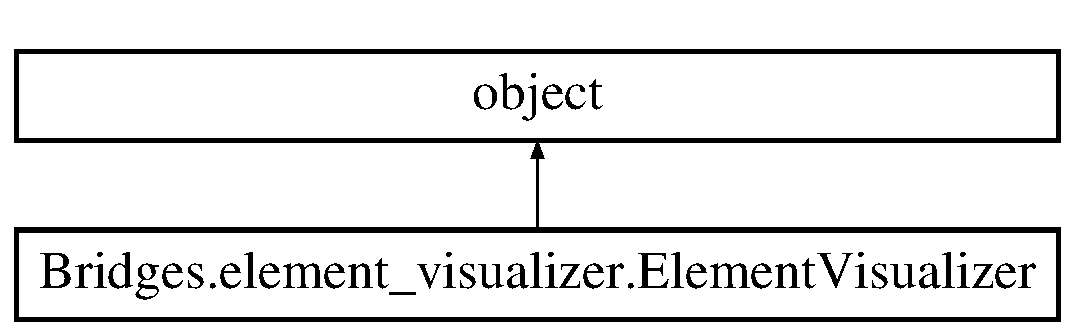
\includegraphics[height=2.000000cm]{class_bridges_1_1element__visualizer_1_1_element_visualizer}
\end{center}
\end{figure}
\subsection*{Public Member Functions}
\begin{DoxyCompactItemize}
\item 
def \mbox{\hyperlink{class_bridges_1_1element__visualizer_1_1_element_visualizer_a8b7a117ef735871e09cac605f0b71c1c}{\+\_\+\+\_\+init\+\_\+\+\_\+}} (self, a\+\_\+color=\char`\"{}green\char`\"{}, a\+\_\+shape=\char`\"{}circle\char`\"{}, size=10.\+0, \mbox{\hyperlink{class_bridges_1_1element__visualizer_1_1_element_visualizer_a8c32a4ec0b2de8d90dc9ba32a60d3d31}{opacity}}=1.\+0)
\begin{DoxyCompactList}\small\item\em Construct an \mbox{\hyperlink{class_bridges_1_1element__visualizer_1_1_element_visualizer}{Element\+Visualizer}} with the default visualization settings. \end{DoxyCompactList}\item 
def \mbox{\hyperlink{class_bridges_1_1element__visualizer_1_1_element_visualizer_ad3d6b884bca4cd65a300d7ca5a9a6ebb}{set\+\_\+size}} (self, \mbox{\hyperlink{class_bridges_1_1element__visualizer_1_1_element_visualizer_a310edf0712e14c6d01264ca050166872}{size}})
\begin{DoxyCompactList}\small\item\em Set the size of the Element in the Bridge Visualization in pixels. \end{DoxyCompactList}\item 
def \mbox{\hyperlink{class_bridges_1_1element__visualizer_1_1_element_visualizer_a43e24d7977692b676da745c9a775c2d7}{get\+\_\+size}} (self)
\begin{DoxyCompactList}\small\item\em Get the size of the Element in the bridges Visualiation. \end{DoxyCompactList}\item 
def \mbox{\hyperlink{class_bridges_1_1element__visualizer_1_1_element_visualizer_a5dceeba34842559488e0fca0013d97eb}{set\+\_\+color}} (self, args, kwargs)
\begin{DoxyCompactList}\small\item\em Set the color of the Element in the bridges Visualization to \char`\"{}a\+Color\char`\"{}. \end{DoxyCompactList}\item 
def \mbox{\hyperlink{class_bridges_1_1element__visualizer_1_1_element_visualizer_a9609a09051cba296c42be588786be4da}{get\+\_\+color}} (self)
\begin{DoxyCompactList}\small\item\em Get the color of the Element in the bridges Visualization. \end{DoxyCompactList}\item 
def \mbox{\hyperlink{class_bridges_1_1element__visualizer_1_1_element_visualizer_af897973bc87f21bb93149a820d6f32f5}{get\+\_\+shape}} (self)
\begin{DoxyCompactList}\small\item\em Get the shape of the Element in the bridges Visualization. \end{DoxyCompactList}\item 
def \mbox{\hyperlink{class_bridges_1_1element__visualizer_1_1_element_visualizer_a577c5842df4a7156bca91b19a8b1ccd5}{set\+\_\+shape}} (self, a\+\_\+shape)
\begin{DoxyCompactList}\small\item\em Sets the shape of the Element in the bridges Visualization. \end{DoxyCompactList}\item 
def \mbox{\hyperlink{class_bridges_1_1element__visualizer_1_1_element_visualizer_a16a1f22e7033c940d7b9cd5b4d0bc67c}{set\+\_\+opacity}} (self, \mbox{\hyperlink{class_bridges_1_1element__visualizer_1_1_element_visualizer_a8c32a4ec0b2de8d90dc9ba32a60d3d31}{opacity}})
\begin{DoxyCompactList}\small\item\em Sets the opacity of the Element in the bridges Visualization. \end{DoxyCompactList}\item 
def \mbox{\hyperlink{class_bridges_1_1element__visualizer_1_1_element_visualizer_a6976f47d3efbec8f7143ff865590c717}{get\+\_\+opacity}} (self)
\begin{DoxyCompactList}\small\item\em Get the opacity of the Element in the bridges Visualization. \end{DoxyCompactList}\item 
def \mbox{\hyperlink{class_bridges_1_1element__visualizer_1_1_element_visualizer_ad383e4865437f64afa039924658d49ba}{set\+\_\+location}} (self, x, y)
\begin{DoxyCompactList}\small\item\em The random\+Color method selects a random color from the available list of colors found in Validation.\+java and sets the color of the current element. \end{DoxyCompactList}\item 
def \mbox{\hyperlink{class_bridges_1_1element__visualizer_1_1_element_visualizer_a25986dc0ad3ec89dd8a933bd4ff782cc}{get\+\_\+locationX}} (self)
\item 
def \mbox{\hyperlink{class_bridges_1_1element__visualizer_1_1_element_visualizer_a5edeca0b69cd6c4457148170058147f1}{get\+\_\+locationY}} (self)
\end{DoxyCompactItemize}
\subsection*{Public Attributes}
\begin{DoxyCompactItemize}
\item 
\mbox{\hyperlink{class_bridges_1_1element__visualizer_1_1_element_visualizer_adb59ea72f9824578f3c2e8946dd4d588}{color}}
\item 
\mbox{\hyperlink{class_bridges_1_1element__visualizer_1_1_element_visualizer_accfe9e47f83d470165a8bfa8d1ef57c2}{size}}
\item 
\mbox{\hyperlink{class_bridges_1_1element__visualizer_1_1_element_visualizer_adb388088c26e6d232e3eb1e01f4c1bb6}{shape}}
\item 
\mbox{\hyperlink{class_bridges_1_1element__visualizer_1_1_element_visualizer_a8dff1d79beb3adc84e1f7a2d251415f3}{opacity}}
\end{DoxyCompactItemize}
\subsection*{Static Public Attributes}
\begin{DoxyCompactItemize}
\item 
string \mbox{\hyperlink{class_bridges_1_1element__visualizer_1_1_element_visualizer_a5bd4e1803cba20426bd7cb60edcee420}{shape}} = \char`\"{}circle\char`\"{}
\item 
string \mbox{\hyperlink{class_bridges_1_1element__visualizer_1_1_element_visualizer_a7fca8f05f8ca3cab859616f0343a7c5d}{key}} = \char`\"{}\char`\"{}
\item 
\mbox{\hyperlink{class_bridges_1_1element__visualizer_1_1_element_visualizer_a51873c21c714a0a309254417ced7feee}{locationX}} = Decimal(\char`\"{}Infinity\char`\"{})
\item 
\mbox{\hyperlink{class_bridges_1_1element__visualizer_1_1_element_visualizer_a59ea4d6ddad480cc3d014914cf64c35e}{locationY}} = Decimal(\char`\"{}Infinity\char`\"{})
\item 
float \mbox{\hyperlink{class_bridges_1_1element__visualizer_1_1_element_visualizer_a310edf0712e14c6d01264ca050166872}{size}} = 10.\+0
\item 
float \mbox{\hyperlink{class_bridges_1_1element__visualizer_1_1_element_visualizer_a8c32a4ec0b2de8d90dc9ba32a60d3d31}{opacity}} = 1.\+0
\item 
\mbox{\hyperlink{class_bridges_1_1element__visualizer_1_1_element_visualizer_a9eabc54da2fc1d0d04b9959d853cadbd}{prop}} = dict()
\end{DoxyCompactItemize}


\subsection{Detailed Description}
This class is used to store the visualization elements on the for the bridges Visualiztion, including the color, shape, opacity, and size of the node. 

Objects of this class are stored as properties of all Element subclasses. Generally, you will manipulating the \mbox{\hyperlink{class_bridges_1_1element__visualizer_1_1_element_visualizer}{Element\+Visualizer}} returned from the Element get\+Visualizer() method, and then call the set\+Visualizer() method on the Element after changes have been made. 

\subsection{Constructor \& Destructor Documentation}
\mbox{\Hypertarget{class_bridges_1_1element__visualizer_1_1_element_visualizer_a8b7a117ef735871e09cac605f0b71c1c}\label{class_bridges_1_1element__visualizer_1_1_element_visualizer_a8b7a117ef735871e09cac605f0b71c1c}} 
\index{Bridges\+::element\+\_\+visualizer\+::\+Element\+Visualizer@{Bridges\+::element\+\_\+visualizer\+::\+Element\+Visualizer}!\+\_\+\+\_\+init\+\_\+\+\_\+@{\+\_\+\+\_\+init\+\_\+\+\_\+}}
\index{\+\_\+\+\_\+init\+\_\+\+\_\+@{\+\_\+\+\_\+init\+\_\+\+\_\+}!Bridges\+::element\+\_\+visualizer\+::\+Element\+Visualizer@{Bridges\+::element\+\_\+visualizer\+::\+Element\+Visualizer}}
\subsubsection{\texorpdfstring{\+\_\+\+\_\+init\+\_\+\+\_\+()}{\_\_init\_\_()}}
{\footnotesize\ttfamily def Bridges.\+element\+\_\+visualizer.\+Element\+Visualizer.\+\_\+\+\_\+init\+\_\+\+\_\+ (\begin{DoxyParamCaption}\item[{}]{self,  }\item[{}]{a\+\_\+color = {\ttfamily \char`\"{}green\char`\"{}},  }\item[{}]{a\+\_\+shape = {\ttfamily \char`\"{}circle\char`\"{}},  }\item[{}]{size = {\ttfamily 10.0},  }\item[{}]{opacity = {\ttfamily 1.0} }\end{DoxyParamCaption})}



Construct an \mbox{\hyperlink{class_bridges_1_1element__visualizer_1_1_element_visualizer}{Element\+Visualizer}} with the default visualization settings. 

The default settings are color = green, opacity = 1.\+0, size = 10.\+0, shape = circle. 

\subsection{Member Function Documentation}
\mbox{\Hypertarget{class_bridges_1_1element__visualizer_1_1_element_visualizer_a9609a09051cba296c42be588786be4da}\label{class_bridges_1_1element__visualizer_1_1_element_visualizer_a9609a09051cba296c42be588786be4da}} 
\index{Bridges\+::element\+\_\+visualizer\+::\+Element\+Visualizer@{Bridges\+::element\+\_\+visualizer\+::\+Element\+Visualizer}!get\+\_\+color@{get\+\_\+color}}
\index{get\+\_\+color@{get\+\_\+color}!Bridges\+::element\+\_\+visualizer\+::\+Element\+Visualizer@{Bridges\+::element\+\_\+visualizer\+::\+Element\+Visualizer}}
\subsubsection{\texorpdfstring{get\+\_\+color()}{get\_color()}}
{\footnotesize\ttfamily def Bridges.\+element\+\_\+visualizer.\+Element\+Visualizer.\+get\+\_\+color (\begin{DoxyParamCaption}\item[{}]{self }\end{DoxyParamCaption})}



Get the color of the Element in the bridges Visualization. 

\begin{DoxyReturn}{Returns}
the string reprsenting the color of the Element in the bridges Visualization 
\end{DoxyReturn}
\mbox{\Hypertarget{class_bridges_1_1element__visualizer_1_1_element_visualizer_a25986dc0ad3ec89dd8a933bd4ff782cc}\label{class_bridges_1_1element__visualizer_1_1_element_visualizer_a25986dc0ad3ec89dd8a933bd4ff782cc}} 
\index{Bridges\+::element\+\_\+visualizer\+::\+Element\+Visualizer@{Bridges\+::element\+\_\+visualizer\+::\+Element\+Visualizer}!get\+\_\+locationX@{get\+\_\+locationX}}
\index{get\+\_\+locationX@{get\+\_\+locationX}!Bridges\+::element\+\_\+visualizer\+::\+Element\+Visualizer@{Bridges\+::element\+\_\+visualizer\+::\+Element\+Visualizer}}
\subsubsection{\texorpdfstring{get\+\_\+location\+X()}{get\_locationX()}}
{\footnotesize\ttfamily def Bridges.\+element\+\_\+visualizer.\+Element\+Visualizer.\+get\+\_\+locationX (\begin{DoxyParamCaption}\item[{}]{self }\end{DoxyParamCaption})}

\mbox{\Hypertarget{class_bridges_1_1element__visualizer_1_1_element_visualizer_a5edeca0b69cd6c4457148170058147f1}\label{class_bridges_1_1element__visualizer_1_1_element_visualizer_a5edeca0b69cd6c4457148170058147f1}} 
\index{Bridges\+::element\+\_\+visualizer\+::\+Element\+Visualizer@{Bridges\+::element\+\_\+visualizer\+::\+Element\+Visualizer}!get\+\_\+locationY@{get\+\_\+locationY}}
\index{get\+\_\+locationY@{get\+\_\+locationY}!Bridges\+::element\+\_\+visualizer\+::\+Element\+Visualizer@{Bridges\+::element\+\_\+visualizer\+::\+Element\+Visualizer}}
\subsubsection{\texorpdfstring{get\+\_\+location\+Y()}{get\_locationY()}}
{\footnotesize\ttfamily def Bridges.\+element\+\_\+visualizer.\+Element\+Visualizer.\+get\+\_\+locationY (\begin{DoxyParamCaption}\item[{}]{self }\end{DoxyParamCaption})}

\mbox{\Hypertarget{class_bridges_1_1element__visualizer_1_1_element_visualizer_a6976f47d3efbec8f7143ff865590c717}\label{class_bridges_1_1element__visualizer_1_1_element_visualizer_a6976f47d3efbec8f7143ff865590c717}} 
\index{Bridges\+::element\+\_\+visualizer\+::\+Element\+Visualizer@{Bridges\+::element\+\_\+visualizer\+::\+Element\+Visualizer}!get\+\_\+opacity@{get\+\_\+opacity}}
\index{get\+\_\+opacity@{get\+\_\+opacity}!Bridges\+::element\+\_\+visualizer\+::\+Element\+Visualizer@{Bridges\+::element\+\_\+visualizer\+::\+Element\+Visualizer}}
\subsubsection{\texorpdfstring{get\+\_\+opacity()}{get\_opacity()}}
{\footnotesize\ttfamily def Bridges.\+element\+\_\+visualizer.\+Element\+Visualizer.\+get\+\_\+opacity (\begin{DoxyParamCaption}\item[{}]{self }\end{DoxyParamCaption})}



Get the opacity of the Element in the bridges Visualization. 

\begin{DoxyReturn}{Returns}
the opacity value 
\end{DoxyReturn}
\mbox{\Hypertarget{class_bridges_1_1element__visualizer_1_1_element_visualizer_af897973bc87f21bb93149a820d6f32f5}\label{class_bridges_1_1element__visualizer_1_1_element_visualizer_af897973bc87f21bb93149a820d6f32f5}} 
\index{Bridges\+::element\+\_\+visualizer\+::\+Element\+Visualizer@{Bridges\+::element\+\_\+visualizer\+::\+Element\+Visualizer}!get\+\_\+shape@{get\+\_\+shape}}
\index{get\+\_\+shape@{get\+\_\+shape}!Bridges\+::element\+\_\+visualizer\+::\+Element\+Visualizer@{Bridges\+::element\+\_\+visualizer\+::\+Element\+Visualizer}}
\subsubsection{\texorpdfstring{get\+\_\+shape()}{get\_shape()}}
{\footnotesize\ttfamily def Bridges.\+element\+\_\+visualizer.\+Element\+Visualizer.\+get\+\_\+shape (\begin{DoxyParamCaption}\item[{}]{self }\end{DoxyParamCaption})}



Get the shape of the Element in the bridges Visualization. 

\begin{DoxyReturn}{Returns}
the string that represents the Element\textquotesingle{}s shape in the bridges Visualization. 
\end{DoxyReturn}
\mbox{\Hypertarget{class_bridges_1_1element__visualizer_1_1_element_visualizer_a43e24d7977692b676da745c9a775c2d7}\label{class_bridges_1_1element__visualizer_1_1_element_visualizer_a43e24d7977692b676da745c9a775c2d7}} 
\index{Bridges\+::element\+\_\+visualizer\+::\+Element\+Visualizer@{Bridges\+::element\+\_\+visualizer\+::\+Element\+Visualizer}!get\+\_\+size@{get\+\_\+size}}
\index{get\+\_\+size@{get\+\_\+size}!Bridges\+::element\+\_\+visualizer\+::\+Element\+Visualizer@{Bridges\+::element\+\_\+visualizer\+::\+Element\+Visualizer}}
\subsubsection{\texorpdfstring{get\+\_\+size()}{get\_size()}}
{\footnotesize\ttfamily def Bridges.\+element\+\_\+visualizer.\+Element\+Visualizer.\+get\+\_\+size (\begin{DoxyParamCaption}\item[{}]{self }\end{DoxyParamCaption})}



Get the size of the Element in the bridges Visualiation. 

\begin{DoxyReturn}{Returns}
the size in pixels of the Element in the bridges Visualization 
\end{DoxyReturn}
\mbox{\Hypertarget{class_bridges_1_1element__visualizer_1_1_element_visualizer_a5dceeba34842559488e0fca0013d97eb}\label{class_bridges_1_1element__visualizer_1_1_element_visualizer_a5dceeba34842559488e0fca0013d97eb}} 
\index{Bridges\+::element\+\_\+visualizer\+::\+Element\+Visualizer@{Bridges\+::element\+\_\+visualizer\+::\+Element\+Visualizer}!set\+\_\+color@{set\+\_\+color}}
\index{set\+\_\+color@{set\+\_\+color}!Bridges\+::element\+\_\+visualizer\+::\+Element\+Visualizer@{Bridges\+::element\+\_\+visualizer\+::\+Element\+Visualizer}}
\subsubsection{\texorpdfstring{set\+\_\+color()}{set\_color()}}
{\footnotesize\ttfamily def Bridges.\+element\+\_\+visualizer.\+Element\+Visualizer.\+set\+\_\+color (\begin{DoxyParamCaption}\item[{}]{self,  }\item[{}]{args,  }\item[{}]{kwargs }\end{DoxyParamCaption})}



Set the color of the Element in the bridges Visualization to \char`\"{}a\+Color\char`\"{}. 


\begin{DoxyParams}{Parameters}
{\em a\+Color} & the string reprsenting the color of the Element in the bridges Visualization\begin{DoxyVerb}Usage: requires either 3 ints 0-255 for RGB and an optional float 0.0-1.0 for alpha or a str of a web color
can also key the RGBA values with r, g, b, a or red, green, blue, alpha respectively and col_name for the str
:param args: int, int, int optional float or str
:param kwargs: r/red: int, b/blue: int, g/green: int optional a/alpha: float or col_name: str
:return: None
\end{DoxyVerb}
 \\
\hline
\end{DoxyParams}
\mbox{\Hypertarget{class_bridges_1_1element__visualizer_1_1_element_visualizer_ad383e4865437f64afa039924658d49ba}\label{class_bridges_1_1element__visualizer_1_1_element_visualizer_ad383e4865437f64afa039924658d49ba}} 
\index{Bridges\+::element\+\_\+visualizer\+::\+Element\+Visualizer@{Bridges\+::element\+\_\+visualizer\+::\+Element\+Visualizer}!set\+\_\+location@{set\+\_\+location}}
\index{set\+\_\+location@{set\+\_\+location}!Bridges\+::element\+\_\+visualizer\+::\+Element\+Visualizer@{Bridges\+::element\+\_\+visualizer\+::\+Element\+Visualizer}}
\subsubsection{\texorpdfstring{set\+\_\+location()}{set\_location()}}
{\footnotesize\ttfamily def Bridges.\+element\+\_\+visualizer.\+Element\+Visualizer.\+set\+\_\+location (\begin{DoxyParamCaption}\item[{}]{self,  }\item[{}]{x,  }\item[{}]{y }\end{DoxyParamCaption})}



The random\+Color method selects a random color from the available list of colors found in Validation.\+java and sets the color of the current element. 

\begin{DoxyReturn}{Returns}
a color name as a string value
\end{DoxyReturn}
def random\+\_\+color(self)\+: a = Validation.\+C\+O\+L\+O\+R\+\_\+\+N\+A\+M\+E\+S.\+to\+Array() return self.\+set\+Color(a\mbox{[}Random().next\+Int(a.\+length)\mbox{]}.\+\_\+\+\_\+str\+\_\+\+\_\+()) \mbox{\Hypertarget{class_bridges_1_1element__visualizer_1_1_element_visualizer_a16a1f22e7033c940d7b9cd5b4d0bc67c}\label{class_bridges_1_1element__visualizer_1_1_element_visualizer_a16a1f22e7033c940d7b9cd5b4d0bc67c}} 
\index{Bridges\+::element\+\_\+visualizer\+::\+Element\+Visualizer@{Bridges\+::element\+\_\+visualizer\+::\+Element\+Visualizer}!set\+\_\+opacity@{set\+\_\+opacity}}
\index{set\+\_\+opacity@{set\+\_\+opacity}!Bridges\+::element\+\_\+visualizer\+::\+Element\+Visualizer@{Bridges\+::element\+\_\+visualizer\+::\+Element\+Visualizer}}
\subsubsection{\texorpdfstring{set\+\_\+opacity()}{set\_opacity()}}
{\footnotesize\ttfamily def Bridges.\+element\+\_\+visualizer.\+Element\+Visualizer.\+set\+\_\+opacity (\begin{DoxyParamCaption}\item[{}]{self,  }\item[{}]{opacity }\end{DoxyParamCaption})}



Sets the opacity of the Element in the bridges Visualization. 


\begin{DoxyParams}{Parameters}
{\em opacity} & a double between 0 and 1 representing how transparent the node should be on the bridges Visualization. 0 for invisible, 1 for fully visible, a decimal between 0 and 1 for varying transparency. \\
\hline
\end{DoxyParams}
\mbox{\Hypertarget{class_bridges_1_1element__visualizer_1_1_element_visualizer_a577c5842df4a7156bca91b19a8b1ccd5}\label{class_bridges_1_1element__visualizer_1_1_element_visualizer_a577c5842df4a7156bca91b19a8b1ccd5}} 
\index{Bridges\+::element\+\_\+visualizer\+::\+Element\+Visualizer@{Bridges\+::element\+\_\+visualizer\+::\+Element\+Visualizer}!set\+\_\+shape@{set\+\_\+shape}}
\index{set\+\_\+shape@{set\+\_\+shape}!Bridges\+::element\+\_\+visualizer\+::\+Element\+Visualizer@{Bridges\+::element\+\_\+visualizer\+::\+Element\+Visualizer}}
\subsubsection{\texorpdfstring{set\+\_\+shape()}{set\_shape()}}
{\footnotesize\ttfamily def Bridges.\+element\+\_\+visualizer.\+Element\+Visualizer.\+set\+\_\+shape (\begin{DoxyParamCaption}\item[{}]{self,  }\item[{}]{a\+\_\+shape }\end{DoxyParamCaption})}



Sets the shape of the Element in the bridges Visualization. 


\begin{DoxyParams}{Parameters}
{\em a\+Shape} & the string representing the shape of the Element in the bridges Visualization \\
\hline
\end{DoxyParams}
\mbox{\Hypertarget{class_bridges_1_1element__visualizer_1_1_element_visualizer_ad3d6b884bca4cd65a300d7ca5a9a6ebb}\label{class_bridges_1_1element__visualizer_1_1_element_visualizer_ad3d6b884bca4cd65a300d7ca5a9a6ebb}} 
\index{Bridges\+::element\+\_\+visualizer\+::\+Element\+Visualizer@{Bridges\+::element\+\_\+visualizer\+::\+Element\+Visualizer}!set\+\_\+size@{set\+\_\+size}}
\index{set\+\_\+size@{set\+\_\+size}!Bridges\+::element\+\_\+visualizer\+::\+Element\+Visualizer@{Bridges\+::element\+\_\+visualizer\+::\+Element\+Visualizer}}
\subsubsection{\texorpdfstring{set\+\_\+size()}{set\_size()}}
{\footnotesize\ttfamily def Bridges.\+element\+\_\+visualizer.\+Element\+Visualizer.\+set\+\_\+size (\begin{DoxyParamCaption}\item[{}]{self,  }\item[{}]{size }\end{DoxyParamCaption})}



Set the size of the Element in the Bridge Visualization in pixels. 


\begin{DoxyParams}{Parameters}
{\em size} & the pixel size of the Element in the bridges Visualization \\
\hline
\end{DoxyParams}


\subsection{Member Data Documentation}
\mbox{\Hypertarget{class_bridges_1_1element__visualizer_1_1_element_visualizer_adb59ea72f9824578f3c2e8946dd4d588}\label{class_bridges_1_1element__visualizer_1_1_element_visualizer_adb59ea72f9824578f3c2e8946dd4d588}} 
\index{Bridges\+::element\+\_\+visualizer\+::\+Element\+Visualizer@{Bridges\+::element\+\_\+visualizer\+::\+Element\+Visualizer}!color@{color}}
\index{color@{color}!Bridges\+::element\+\_\+visualizer\+::\+Element\+Visualizer@{Bridges\+::element\+\_\+visualizer\+::\+Element\+Visualizer}}
\subsubsection{\texorpdfstring{color}{color}}
{\footnotesize\ttfamily Bridges.\+element\+\_\+visualizer.\+Element\+Visualizer.\+color}

\mbox{\Hypertarget{class_bridges_1_1element__visualizer_1_1_element_visualizer_a7fca8f05f8ca3cab859616f0343a7c5d}\label{class_bridges_1_1element__visualizer_1_1_element_visualizer_a7fca8f05f8ca3cab859616f0343a7c5d}} 
\index{Bridges\+::element\+\_\+visualizer\+::\+Element\+Visualizer@{Bridges\+::element\+\_\+visualizer\+::\+Element\+Visualizer}!key@{key}}
\index{key@{key}!Bridges\+::element\+\_\+visualizer\+::\+Element\+Visualizer@{Bridges\+::element\+\_\+visualizer\+::\+Element\+Visualizer}}
\subsubsection{\texorpdfstring{key}{key}}
{\footnotesize\ttfamily string Bridges.\+element\+\_\+visualizer.\+Element\+Visualizer.\+key = \char`\"{}\char`\"{}\hspace{0.3cm}{\ttfamily [static]}}

\mbox{\Hypertarget{class_bridges_1_1element__visualizer_1_1_element_visualizer_a51873c21c714a0a309254417ced7feee}\label{class_bridges_1_1element__visualizer_1_1_element_visualizer_a51873c21c714a0a309254417ced7feee}} 
\index{Bridges\+::element\+\_\+visualizer\+::\+Element\+Visualizer@{Bridges\+::element\+\_\+visualizer\+::\+Element\+Visualizer}!locationX@{locationX}}
\index{locationX@{locationX}!Bridges\+::element\+\_\+visualizer\+::\+Element\+Visualizer@{Bridges\+::element\+\_\+visualizer\+::\+Element\+Visualizer}}
\subsubsection{\texorpdfstring{locationX}{locationX}}
{\footnotesize\ttfamily Bridges.\+element\+\_\+visualizer.\+Element\+Visualizer.\+locationX = Decimal(\char`\"{}Infinity\char`\"{})\hspace{0.3cm}{\ttfamily [static]}}

\mbox{\Hypertarget{class_bridges_1_1element__visualizer_1_1_element_visualizer_a59ea4d6ddad480cc3d014914cf64c35e}\label{class_bridges_1_1element__visualizer_1_1_element_visualizer_a59ea4d6ddad480cc3d014914cf64c35e}} 
\index{Bridges\+::element\+\_\+visualizer\+::\+Element\+Visualizer@{Bridges\+::element\+\_\+visualizer\+::\+Element\+Visualizer}!locationY@{locationY}}
\index{locationY@{locationY}!Bridges\+::element\+\_\+visualizer\+::\+Element\+Visualizer@{Bridges\+::element\+\_\+visualizer\+::\+Element\+Visualizer}}
\subsubsection{\texorpdfstring{locationY}{locationY}}
{\footnotesize\ttfamily Bridges.\+element\+\_\+visualizer.\+Element\+Visualizer.\+locationY = Decimal(\char`\"{}Infinity\char`\"{})\hspace{0.3cm}{\ttfamily [static]}}

\mbox{\Hypertarget{class_bridges_1_1element__visualizer_1_1_element_visualizer_a8c32a4ec0b2de8d90dc9ba32a60d3d31}\label{class_bridges_1_1element__visualizer_1_1_element_visualizer_a8c32a4ec0b2de8d90dc9ba32a60d3d31}} 
\index{Bridges\+::element\+\_\+visualizer\+::\+Element\+Visualizer@{Bridges\+::element\+\_\+visualizer\+::\+Element\+Visualizer}!opacity@{opacity}}
\index{opacity@{opacity}!Bridges\+::element\+\_\+visualizer\+::\+Element\+Visualizer@{Bridges\+::element\+\_\+visualizer\+::\+Element\+Visualizer}}
\subsubsection{\texorpdfstring{opacity}{opacity}\hspace{0.1cm}{\footnotesize\ttfamily [1/2]}}
{\footnotesize\ttfamily float Bridges.\+element\+\_\+visualizer.\+Element\+Visualizer.\+opacity = 1.\+0\hspace{0.3cm}{\ttfamily [static]}}

\mbox{\Hypertarget{class_bridges_1_1element__visualizer_1_1_element_visualizer_a8dff1d79beb3adc84e1f7a2d251415f3}\label{class_bridges_1_1element__visualizer_1_1_element_visualizer_a8dff1d79beb3adc84e1f7a2d251415f3}} 
\index{Bridges\+::element\+\_\+visualizer\+::\+Element\+Visualizer@{Bridges\+::element\+\_\+visualizer\+::\+Element\+Visualizer}!opacity@{opacity}}
\index{opacity@{opacity}!Bridges\+::element\+\_\+visualizer\+::\+Element\+Visualizer@{Bridges\+::element\+\_\+visualizer\+::\+Element\+Visualizer}}
\subsubsection{\texorpdfstring{opacity}{opacity}\hspace{0.1cm}{\footnotesize\ttfamily [2/2]}}
{\footnotesize\ttfamily Bridges.\+element\+\_\+visualizer.\+Element\+Visualizer.\+opacity}

\mbox{\Hypertarget{class_bridges_1_1element__visualizer_1_1_element_visualizer_a9eabc54da2fc1d0d04b9959d853cadbd}\label{class_bridges_1_1element__visualizer_1_1_element_visualizer_a9eabc54da2fc1d0d04b9959d853cadbd}} 
\index{Bridges\+::element\+\_\+visualizer\+::\+Element\+Visualizer@{Bridges\+::element\+\_\+visualizer\+::\+Element\+Visualizer}!prop@{prop}}
\index{prop@{prop}!Bridges\+::element\+\_\+visualizer\+::\+Element\+Visualizer@{Bridges\+::element\+\_\+visualizer\+::\+Element\+Visualizer}}
\subsubsection{\texorpdfstring{prop}{prop}}
{\footnotesize\ttfamily Bridges.\+element\+\_\+visualizer.\+Element\+Visualizer.\+prop = dict()\hspace{0.3cm}{\ttfamily [static]}}

\mbox{\Hypertarget{class_bridges_1_1element__visualizer_1_1_element_visualizer_a5bd4e1803cba20426bd7cb60edcee420}\label{class_bridges_1_1element__visualizer_1_1_element_visualizer_a5bd4e1803cba20426bd7cb60edcee420}} 
\index{Bridges\+::element\+\_\+visualizer\+::\+Element\+Visualizer@{Bridges\+::element\+\_\+visualizer\+::\+Element\+Visualizer}!shape@{shape}}
\index{shape@{shape}!Bridges\+::element\+\_\+visualizer\+::\+Element\+Visualizer@{Bridges\+::element\+\_\+visualizer\+::\+Element\+Visualizer}}
\subsubsection{\texorpdfstring{shape}{shape}\hspace{0.1cm}{\footnotesize\ttfamily [1/2]}}
{\footnotesize\ttfamily string Bridges.\+element\+\_\+visualizer.\+Element\+Visualizer.\+shape = \char`\"{}circle\char`\"{}\hspace{0.3cm}{\ttfamily [static]}}

\mbox{\Hypertarget{class_bridges_1_1element__visualizer_1_1_element_visualizer_adb388088c26e6d232e3eb1e01f4c1bb6}\label{class_bridges_1_1element__visualizer_1_1_element_visualizer_adb388088c26e6d232e3eb1e01f4c1bb6}} 
\index{Bridges\+::element\+\_\+visualizer\+::\+Element\+Visualizer@{Bridges\+::element\+\_\+visualizer\+::\+Element\+Visualizer}!shape@{shape}}
\index{shape@{shape}!Bridges\+::element\+\_\+visualizer\+::\+Element\+Visualizer@{Bridges\+::element\+\_\+visualizer\+::\+Element\+Visualizer}}
\subsubsection{\texorpdfstring{shape}{shape}\hspace{0.1cm}{\footnotesize\ttfamily [2/2]}}
{\footnotesize\ttfamily Bridges.\+element\+\_\+visualizer.\+Element\+Visualizer.\+shape}

\mbox{\Hypertarget{class_bridges_1_1element__visualizer_1_1_element_visualizer_a310edf0712e14c6d01264ca050166872}\label{class_bridges_1_1element__visualizer_1_1_element_visualizer_a310edf0712e14c6d01264ca050166872}} 
\index{Bridges\+::element\+\_\+visualizer\+::\+Element\+Visualizer@{Bridges\+::element\+\_\+visualizer\+::\+Element\+Visualizer}!size@{size}}
\index{size@{size}!Bridges\+::element\+\_\+visualizer\+::\+Element\+Visualizer@{Bridges\+::element\+\_\+visualizer\+::\+Element\+Visualizer}}
\subsubsection{\texorpdfstring{size}{size}\hspace{0.1cm}{\footnotesize\ttfamily [1/2]}}
{\footnotesize\ttfamily float Bridges.\+element\+\_\+visualizer.\+Element\+Visualizer.\+size = 10.\+0\hspace{0.3cm}{\ttfamily [static]}}

\mbox{\Hypertarget{class_bridges_1_1element__visualizer_1_1_element_visualizer_accfe9e47f83d470165a8bfa8d1ef57c2}\label{class_bridges_1_1element__visualizer_1_1_element_visualizer_accfe9e47f83d470165a8bfa8d1ef57c2}} 
\index{Bridges\+::element\+\_\+visualizer\+::\+Element\+Visualizer@{Bridges\+::element\+\_\+visualizer\+::\+Element\+Visualizer}!size@{size}}
\index{size@{size}!Bridges\+::element\+\_\+visualizer\+::\+Element\+Visualizer@{Bridges\+::element\+\_\+visualizer\+::\+Element\+Visualizer}}
\subsubsection{\texorpdfstring{size}{size}\hspace{0.1cm}{\footnotesize\ttfamily [2/2]}}
{\footnotesize\ttfamily Bridges.\+element\+\_\+visualizer.\+Element\+Visualizer.\+size}



The documentation for this class was generated from the following file\+:\begin{DoxyCompactItemize}
\item 
/\+Users/kalpathi/gr/bridges/client/python/bridges18/\+Bridges/\mbox{\hyperlink{element__visualizer_8py}{element\+\_\+visualizer.\+py}}\end{DoxyCompactItemize}

\hypertarget{class_bridges_1_1graph__adj__list_1_1_graph_adj_list}{}\section{Bridges.\+graph\+\_\+adj\+\_\+list.\+Graph\+Adj\+List Class Reference}
\label{class_bridges_1_1graph__adj__list_1_1_graph_adj_list}\index{Bridges.\+graph\+\_\+adj\+\_\+list.\+Graph\+Adj\+List@{Bridges.\+graph\+\_\+adj\+\_\+list.\+Graph\+Adj\+List}}


The \mbox{\hyperlink{class_bridges_1_1graph__adj__list_1_1_graph_adj_list}{Graph\+Adj\+List}} class can be used to represent adjacency list based graphs in B\+R\+I\+D\+G\+ES.  


\subsection*{Public Member Functions}
\begin{DoxyCompactItemize}
\item 
def \mbox{\hyperlink{class_bridges_1_1graph__adj__list_1_1_graph_adj_list_a38885cb113043d73371b5799271a0150}{\+\_\+\+\_\+init\+\_\+\+\_\+}} (self)
\begin{DoxyCompactList}\small\item\em Constructor. \end{DoxyCompactList}\item 
def \mbox{\hyperlink{class_bridges_1_1graph__adj__list_1_1_graph_adj_list_a3c7457eef2346da45ad0714e07e39d7e}{get\+\_\+data\+\_\+structure\+\_\+type}} (self)
\begin{DoxyCompactList}\small\item\em This method gets the data structure type. \end{DoxyCompactList}\item 
def \mbox{\hyperlink{class_bridges_1_1graph__adj__list_1_1_graph_adj_list_a93fa88e14042ecbf8bf57d4f5e072a72}{add\+\_\+vertex}} (self, k, e)
\begin{DoxyCompactList}\small\item\em Adds a new vertex to the graph, initializes the adjacency list; user is responsible for checking if the vertex already exists. \end{DoxyCompactList}\item 
def \mbox{\hyperlink{class_bridges_1_1graph__adj__list_1_1_graph_adj_list_a6bbe6032852513b0dcc96c32ba9a38d5}{add\+\_\+edge}} (self, src, dest, weight=None)
\begin{DoxyCompactList}\small\item\em Adds a new edge to the graph, adds it to that vertex\textquotesingle{}s adjacency list; user is responsible for checking if the vertex already exists. \end{DoxyCompactList}\item 
def \mbox{\hyperlink{class_bridges_1_1graph__adj__list_1_1_graph_adj_list_a1a7db65bac1524f5d94b7f1387363ce8}{get\+\_\+vertices}} (self)
\begin{DoxyCompactList}\small\item\em This method returns the graph nodes. \end{DoxyCompactList}\item 
def \mbox{\hyperlink{class_bridges_1_1graph__adj__list_1_1_graph_adj_list_a75a7ac26f72d773b40cd5eaa95d18b7a}{get\+\_\+vertex}} (self, key)
\begin{DoxyCompactList}\small\item\em This is a convenience method to retrieve a vertex given its key. \end{DoxyCompactList}\item 
def \mbox{\hyperlink{class_bridges_1_1graph__adj__list_1_1_graph_adj_list_aaec1428d2d56a5f71a47406ac8aa9031}{get\+\_\+adjacency\+\_\+list}} (self, vertex=None)
\begin{DoxyCompactList}\small\item\em Gets the adjacency list (of type S\+Lelement$<$\+Edge$>$ ) \end{DoxyCompactList}\item 
def \mbox{\hyperlink{class_bridges_1_1graph__adj__list_1_1_graph_adj_list_a80a3cacf989d047e20d4ccc83fa550f5}{get\+\_\+link\+\_\+visualizer}} (self, src, dest)
\begin{DoxyCompactList}\small\item\em This is a convenience method to simplify access to the link visualizer; the method assumes the vertex names point to existing vertices, else an exception is thrown. \end{DoxyCompactList}\item 
def \mbox{\hyperlink{class_bridges_1_1graph__adj__list_1_1_graph_adj_list_a854df55aa904a11b37330932772e8690}{get\+\_\+visualizer}} (self, vertex)
\begin{DoxyCompactList}\small\item\em This is a convenience method to simplify access to the element visualizer; the method assumes the vertex name points to an existing vertice, else an exception is thrown. \end{DoxyCompactList}\item 
def \mbox{\hyperlink{class_bridges_1_1graph__adj__list_1_1_graph_adj_list_a63954149a112161a13a259f270f21080}{get\+\_\+data\+\_\+structure\+\_\+representation}} (self)
\begin{DoxyCompactList}\small\item\em Get the J\+S\+ON representation of the the data structure. \end{DoxyCompactList}\end{DoxyCompactItemize}
\subsection*{Public Attributes}
\begin{DoxyCompactItemize}
\item 
\mbox{\hyperlink{class_bridges_1_1graph__adj__list_1_1_graph_adj_list_a3efee49a2137c200d4e21ab28498d209}{vertices}}
\item 
\mbox{\hyperlink{class_bridges_1_1graph__adj__list_1_1_graph_adj_list_a422e14fd0d7ef4fe9c42a790cf635c0f}{adj\+\_\+list}}
\end{DoxyCompactItemize}
\subsection*{Static Public Attributes}
\begin{DoxyCompactItemize}
\item 
string \mbox{\hyperlink{class_bridges_1_1graph__adj__list_1_1_graph_adj_list_a6adf6e943f5fa2d30144a258293caf25}{Q\+U\+O\+TE}} = \char`\"{}\textbackslash{}\char`\"{}\char`\"{}
\item 
string \mbox{\hyperlink{class_bridges_1_1graph__adj__list_1_1_graph_adj_list_a5fcebf83b1ae17db66be51a5d262b842}{C\+O\+M\+MA}} = \char`\"{},\char`\"{}
\item 
string \mbox{\hyperlink{class_bridges_1_1graph__adj__list_1_1_graph_adj_list_a99600a7bd4081501ade877fbe23e1318}{C\+O\+L\+ON}} = \char`\"{}\+:\char`\"{}
\item 
string \mbox{\hyperlink{class_bridges_1_1graph__adj__list_1_1_graph_adj_list_a4e3323194aa0387850dd4c966e6a24a9}{O\+P\+E\+N\+\_\+\+C\+U\+R\+LY}} = \char`\"{}\{\char`\"{}
\item 
string \mbox{\hyperlink{class_bridges_1_1graph__adj__list_1_1_graph_adj_list_ae5bc55f7790bd51ce15e641eb3612c41}{C\+L\+O\+S\+E\+\_\+\+C\+U\+R\+LY}} = \char`\"{}\}\char`\"{}
\item 
string \mbox{\hyperlink{class_bridges_1_1graph__adj__list_1_1_graph_adj_list_aea35b3bb84c38d1d49101c2929b3b73c}{O\+P\+E\+N\+\_\+\+P\+A\+R\+EN}} = \char`\"{}(\char`\"{}
\item 
string \mbox{\hyperlink{class_bridges_1_1graph__adj__list_1_1_graph_adj_list_a94004739bbb4cbdaef3375b1cbde0768}{C\+L\+O\+S\+E\+\_\+\+P\+A\+R\+EN}} = \char`\"{})\char`\"{}
\item 
string \mbox{\hyperlink{class_bridges_1_1graph__adj__list_1_1_graph_adj_list_ae647fcc0ce21e4cbc2c9013e1de0d1c5}{O\+P\+E\+N\+\_\+\+B\+OX}} = \char`\"{}\mbox{[}\char`\"{}
\item 
string \mbox{\hyperlink{class_bridges_1_1graph__adj__list_1_1_graph_adj_list_ad06df79f67b8bba0f397fc2475a3b29f}{C\+L\+O\+S\+E\+\_\+\+B\+OX}} = \char`\"{}\mbox{]}\char`\"{}
\end{DoxyCompactItemize}


\subsection{Detailed Description}
The \mbox{\hyperlink{class_bridges_1_1graph__adj__list_1_1_graph_adj_list}{Graph\+Adj\+List}} class can be used to represent adjacency list based graphs in B\+R\+I\+D\+G\+ES. 

The \mbox{\hyperlink{class_bridges_1_1graph__adj__list_1_1_graph_adj_list}{Graph\+Adj\+List}} class can be used to represent adjacency list based graphs in B\+R\+I\+D\+G\+ES; it takes 2 generic parameters\+: (1) K, which is an orderable key value used in accessing vertices (in constant time) using a hashmap. This permits data sets that need to be accessed by keys that are strings, and (2) E, an application defined type, and used in the Edge representation. The class is simply a wrapper around the Java Hashmap class and, thus, derives all its operations from it. B\+R\+I\+D\+G\+ES provides methods to visualize the graph and its contents.

The vertices of the graph are held in a Java hashmap, for near constant time access; this lets us use strings or integral ids for vertices. The adjacency lists, also a Java hashmap are built for each vertex and contain the edge (terminating vertex id, weight) in the Edge structure, defined separately. Adjacency lists are singly linked lists using the B\+R\+I\+D\+G\+ES S\+Lelement.

Convenience methods are provided to add vertices and edges to the graph as well as retrieve the adjacency list of a vertex, given its id.

\begin{DoxyAuthor}{Author}
Kalpathi Subramanian
\end{DoxyAuthor}
\begin{DoxyVerb}\sa Example tutorial at <p>
    http://bridgesuncc.github.io/Hello_World_Tutorials/Graph.html\end{DoxyVerb}
 

\subsection{Constructor \& Destructor Documentation}
\mbox{\Hypertarget{class_bridges_1_1graph__adj__list_1_1_graph_adj_list_a38885cb113043d73371b5799271a0150}\label{class_bridges_1_1graph__adj__list_1_1_graph_adj_list_a38885cb113043d73371b5799271a0150}} 
\index{Bridges\+::graph\+\_\+adj\+\_\+list\+::\+Graph\+Adj\+List@{Bridges\+::graph\+\_\+adj\+\_\+list\+::\+Graph\+Adj\+List}!\+\_\+\+\_\+init\+\_\+\+\_\+@{\+\_\+\+\_\+init\+\_\+\+\_\+}}
\index{\+\_\+\+\_\+init\+\_\+\+\_\+@{\+\_\+\+\_\+init\+\_\+\+\_\+}!Bridges\+::graph\+\_\+adj\+\_\+list\+::\+Graph\+Adj\+List@{Bridges\+::graph\+\_\+adj\+\_\+list\+::\+Graph\+Adj\+List}}
\subsubsection{\texorpdfstring{\+\_\+\+\_\+init\+\_\+\+\_\+()}{\_\_init\_\_()}}
{\footnotesize\ttfamily def Bridges.\+graph\+\_\+adj\+\_\+list.\+Graph\+Adj\+List.\+\_\+\+\_\+init\+\_\+\+\_\+ (\begin{DoxyParamCaption}\item[{}]{self }\end{DoxyParamCaption})}



Constructor. 



\subsection{Member Function Documentation}
\mbox{\Hypertarget{class_bridges_1_1graph__adj__list_1_1_graph_adj_list_a6bbe6032852513b0dcc96c32ba9a38d5}\label{class_bridges_1_1graph__adj__list_1_1_graph_adj_list_a6bbe6032852513b0dcc96c32ba9a38d5}} 
\index{Bridges\+::graph\+\_\+adj\+\_\+list\+::\+Graph\+Adj\+List@{Bridges\+::graph\+\_\+adj\+\_\+list\+::\+Graph\+Adj\+List}!add\+\_\+edge@{add\+\_\+edge}}
\index{add\+\_\+edge@{add\+\_\+edge}!Bridges\+::graph\+\_\+adj\+\_\+list\+::\+Graph\+Adj\+List@{Bridges\+::graph\+\_\+adj\+\_\+list\+::\+Graph\+Adj\+List}}
\subsubsection{\texorpdfstring{add\+\_\+edge()}{add\_edge()}}
{\footnotesize\ttfamily def Bridges.\+graph\+\_\+adj\+\_\+list.\+Graph\+Adj\+List.\+add\+\_\+edge (\begin{DoxyParamCaption}\item[{}]{self,  }\item[{}]{src,  }\item[{}]{dest,  }\item[{}]{weight = {\ttfamily None} }\end{DoxyParamCaption})}



Adds a new edge to the graph, adds it to that vertex\textquotesingle{}s adjacency list; user is responsible for checking if the vertex already exists. 

This version assumes a default edge weight of 1.


\begin{DoxyParams}{Parameters}
{\em src} & -\/ source vertex of edge \\
\hline
{\em dest} & -\/ destination vertex of edge \\
\hline
\end{DoxyParams}
\mbox{\Hypertarget{class_bridges_1_1graph__adj__list_1_1_graph_adj_list_a93fa88e14042ecbf8bf57d4f5e072a72}\label{class_bridges_1_1graph__adj__list_1_1_graph_adj_list_a93fa88e14042ecbf8bf57d4f5e072a72}} 
\index{Bridges\+::graph\+\_\+adj\+\_\+list\+::\+Graph\+Adj\+List@{Bridges\+::graph\+\_\+adj\+\_\+list\+::\+Graph\+Adj\+List}!add\+\_\+vertex@{add\+\_\+vertex}}
\index{add\+\_\+vertex@{add\+\_\+vertex}!Bridges\+::graph\+\_\+adj\+\_\+list\+::\+Graph\+Adj\+List@{Bridges\+::graph\+\_\+adj\+\_\+list\+::\+Graph\+Adj\+List}}
\subsubsection{\texorpdfstring{add\+\_\+vertex()}{add\_vertex()}}
{\footnotesize\ttfamily def Bridges.\+graph\+\_\+adj\+\_\+list.\+Graph\+Adj\+List.\+add\+\_\+vertex (\begin{DoxyParamCaption}\item[{}]{self,  }\item[{}]{k,  }\item[{}]{e }\end{DoxyParamCaption})}



Adds a new vertex to the graph, initializes the adjacency list; user is responsible for checking if the vertex already exists. 

This method will replace the value for this key


\begin{DoxyParams}{Parameters}
{\em k} & -\/ vertex id \\
\hline
{\em E} & -\/ vertex info, currently used as a label by default \begin{DoxyVerb}@return none\end{DoxyVerb}
 \\
\hline
\end{DoxyParams}
\mbox{\Hypertarget{class_bridges_1_1graph__adj__list_1_1_graph_adj_list_aaec1428d2d56a5f71a47406ac8aa9031}\label{class_bridges_1_1graph__adj__list_1_1_graph_adj_list_aaec1428d2d56a5f71a47406ac8aa9031}} 
\index{Bridges\+::graph\+\_\+adj\+\_\+list\+::\+Graph\+Adj\+List@{Bridges\+::graph\+\_\+adj\+\_\+list\+::\+Graph\+Adj\+List}!get\+\_\+adjacency\+\_\+list@{get\+\_\+adjacency\+\_\+list}}
\index{get\+\_\+adjacency\+\_\+list@{get\+\_\+adjacency\+\_\+list}!Bridges\+::graph\+\_\+adj\+\_\+list\+::\+Graph\+Adj\+List@{Bridges\+::graph\+\_\+adj\+\_\+list\+::\+Graph\+Adj\+List}}
\subsubsection{\texorpdfstring{get\+\_\+adjacency\+\_\+list()}{get\_adjacency\_list()}}
{\footnotesize\ttfamily def Bridges.\+graph\+\_\+adj\+\_\+list.\+Graph\+Adj\+List.\+get\+\_\+adjacency\+\_\+list (\begin{DoxyParamCaption}\item[{}]{self,  }\item[{}]{vertex = {\ttfamily None} }\end{DoxyParamCaption})}



Gets the adjacency list (of type S\+Lelement$<$\+Edge$>$ ) 

\begin{DoxyReturn}{Returns}
-\/ the graph\textquotesingle{}s adjacency lists 
\end{DoxyReturn}
\mbox{\Hypertarget{class_bridges_1_1graph__adj__list_1_1_graph_adj_list_a63954149a112161a13a259f270f21080}\label{class_bridges_1_1graph__adj__list_1_1_graph_adj_list_a63954149a112161a13a259f270f21080}} 
\index{Bridges\+::graph\+\_\+adj\+\_\+list\+::\+Graph\+Adj\+List@{Bridges\+::graph\+\_\+adj\+\_\+list\+::\+Graph\+Adj\+List}!get\+\_\+data\+\_\+structure\+\_\+representation@{get\+\_\+data\+\_\+structure\+\_\+representation}}
\index{get\+\_\+data\+\_\+structure\+\_\+representation@{get\+\_\+data\+\_\+structure\+\_\+representation}!Bridges\+::graph\+\_\+adj\+\_\+list\+::\+Graph\+Adj\+List@{Bridges\+::graph\+\_\+adj\+\_\+list\+::\+Graph\+Adj\+List}}
\subsubsection{\texorpdfstring{get\+\_\+data\+\_\+structure\+\_\+representation()}{get\_data\_structure\_representation()}}
{\footnotesize\ttfamily def Bridges.\+graph\+\_\+adj\+\_\+list.\+Graph\+Adj\+List.\+get\+\_\+data\+\_\+structure\+\_\+representation (\begin{DoxyParamCaption}\item[{}]{self }\end{DoxyParamCaption})}



Get the J\+S\+ON representation of the the data structure. 

\mbox{\Hypertarget{class_bridges_1_1graph__adj__list_1_1_graph_adj_list_a3c7457eef2346da45ad0714e07e39d7e}\label{class_bridges_1_1graph__adj__list_1_1_graph_adj_list_a3c7457eef2346da45ad0714e07e39d7e}} 
\index{Bridges\+::graph\+\_\+adj\+\_\+list\+::\+Graph\+Adj\+List@{Bridges\+::graph\+\_\+adj\+\_\+list\+::\+Graph\+Adj\+List}!get\+\_\+data\+\_\+structure\+\_\+type@{get\+\_\+data\+\_\+structure\+\_\+type}}
\index{get\+\_\+data\+\_\+structure\+\_\+type@{get\+\_\+data\+\_\+structure\+\_\+type}!Bridges\+::graph\+\_\+adj\+\_\+list\+::\+Graph\+Adj\+List@{Bridges\+::graph\+\_\+adj\+\_\+list\+::\+Graph\+Adj\+List}}
\subsubsection{\texorpdfstring{get\+\_\+data\+\_\+structure\+\_\+type()}{get\_data\_structure\_type()}}
{\footnotesize\ttfamily def Bridges.\+graph\+\_\+adj\+\_\+list.\+Graph\+Adj\+List.\+get\+\_\+data\+\_\+structure\+\_\+type (\begin{DoxyParamCaption}\item[{}]{self }\end{DoxyParamCaption})}



This method gets the data structure type. 

\begin{DoxyReturn}{Returns}
The date structure type as a string 
\end{DoxyReturn}
\mbox{\Hypertarget{class_bridges_1_1graph__adj__list_1_1_graph_adj_list_a80a3cacf989d047e20d4ccc83fa550f5}\label{class_bridges_1_1graph__adj__list_1_1_graph_adj_list_a80a3cacf989d047e20d4ccc83fa550f5}} 
\index{Bridges\+::graph\+\_\+adj\+\_\+list\+::\+Graph\+Adj\+List@{Bridges\+::graph\+\_\+adj\+\_\+list\+::\+Graph\+Adj\+List}!get\+\_\+link\+\_\+visualizer@{get\+\_\+link\+\_\+visualizer}}
\index{get\+\_\+link\+\_\+visualizer@{get\+\_\+link\+\_\+visualizer}!Bridges\+::graph\+\_\+adj\+\_\+list\+::\+Graph\+Adj\+List@{Bridges\+::graph\+\_\+adj\+\_\+list\+::\+Graph\+Adj\+List}}
\subsubsection{\texorpdfstring{get\+\_\+link\+\_\+visualizer()}{get\_link\_visualizer()}}
{\footnotesize\ttfamily def Bridges.\+graph\+\_\+adj\+\_\+list.\+Graph\+Adj\+List.\+get\+\_\+link\+\_\+visualizer (\begin{DoxyParamCaption}\item[{}]{self,  }\item[{}]{src,  }\item[{}]{dest }\end{DoxyParamCaption})}



This is a convenience method to simplify access to the link visualizer; the method assumes the vertex names point to existing vertices, else an exception is thrown. 

\mbox{\Hypertarget{class_bridges_1_1graph__adj__list_1_1_graph_adj_list_a75a7ac26f72d773b40cd5eaa95d18b7a}\label{class_bridges_1_1graph__adj__list_1_1_graph_adj_list_a75a7ac26f72d773b40cd5eaa95d18b7a}} 
\index{Bridges\+::graph\+\_\+adj\+\_\+list\+::\+Graph\+Adj\+List@{Bridges\+::graph\+\_\+adj\+\_\+list\+::\+Graph\+Adj\+List}!get\+\_\+vertex@{get\+\_\+vertex}}
\index{get\+\_\+vertex@{get\+\_\+vertex}!Bridges\+::graph\+\_\+adj\+\_\+list\+::\+Graph\+Adj\+List@{Bridges\+::graph\+\_\+adj\+\_\+list\+::\+Graph\+Adj\+List}}
\subsubsection{\texorpdfstring{get\+\_\+vertex()}{get\_vertex()}}
{\footnotesize\ttfamily def Bridges.\+graph\+\_\+adj\+\_\+list.\+Graph\+Adj\+List.\+get\+\_\+vertex (\begin{DoxyParamCaption}\item[{}]{self,  }\item[{}]{key }\end{DoxyParamCaption})}



This is a convenience method to retrieve a vertex given its key. 

return -- graph vertex corresponding to its key \mbox{\Hypertarget{class_bridges_1_1graph__adj__list_1_1_graph_adj_list_a1a7db65bac1524f5d94b7f1387363ce8}\label{class_bridges_1_1graph__adj__list_1_1_graph_adj_list_a1a7db65bac1524f5d94b7f1387363ce8}} 
\index{Bridges\+::graph\+\_\+adj\+\_\+list\+::\+Graph\+Adj\+List@{Bridges\+::graph\+\_\+adj\+\_\+list\+::\+Graph\+Adj\+List}!get\+\_\+vertices@{get\+\_\+vertices}}
\index{get\+\_\+vertices@{get\+\_\+vertices}!Bridges\+::graph\+\_\+adj\+\_\+list\+::\+Graph\+Adj\+List@{Bridges\+::graph\+\_\+adj\+\_\+list\+::\+Graph\+Adj\+List}}
\subsubsection{\texorpdfstring{get\+\_\+vertices()}{get\_vertices()}}
{\footnotesize\ttfamily def Bridges.\+graph\+\_\+adj\+\_\+list.\+Graph\+Adj\+List.\+get\+\_\+vertices (\begin{DoxyParamCaption}\item[{}]{self }\end{DoxyParamCaption})}



This method returns the graph nodes. 

return -- vertices held in in the hashmap \mbox{\Hypertarget{class_bridges_1_1graph__adj__list_1_1_graph_adj_list_a854df55aa904a11b37330932772e8690}\label{class_bridges_1_1graph__adj__list_1_1_graph_adj_list_a854df55aa904a11b37330932772e8690}} 
\index{Bridges\+::graph\+\_\+adj\+\_\+list\+::\+Graph\+Adj\+List@{Bridges\+::graph\+\_\+adj\+\_\+list\+::\+Graph\+Adj\+List}!get\+\_\+visualizer@{get\+\_\+visualizer}}
\index{get\+\_\+visualizer@{get\+\_\+visualizer}!Bridges\+::graph\+\_\+adj\+\_\+list\+::\+Graph\+Adj\+List@{Bridges\+::graph\+\_\+adj\+\_\+list\+::\+Graph\+Adj\+List}}
\subsubsection{\texorpdfstring{get\+\_\+visualizer()}{get\_visualizer()}}
{\footnotesize\ttfamily def Bridges.\+graph\+\_\+adj\+\_\+list.\+Graph\+Adj\+List.\+get\+\_\+visualizer (\begin{DoxyParamCaption}\item[{}]{self,  }\item[{}]{vertex }\end{DoxyParamCaption})}



This is a convenience method to simplify access to the element visualizer; the method assumes the vertex name points to an existing vertice, else an exception is thrown. 



\subsection{Member Data Documentation}
\mbox{\Hypertarget{class_bridges_1_1graph__adj__list_1_1_graph_adj_list_a422e14fd0d7ef4fe9c42a790cf635c0f}\label{class_bridges_1_1graph__adj__list_1_1_graph_adj_list_a422e14fd0d7ef4fe9c42a790cf635c0f}} 
\index{Bridges\+::graph\+\_\+adj\+\_\+list\+::\+Graph\+Adj\+List@{Bridges\+::graph\+\_\+adj\+\_\+list\+::\+Graph\+Adj\+List}!adj\+\_\+list@{adj\+\_\+list}}
\index{adj\+\_\+list@{adj\+\_\+list}!Bridges\+::graph\+\_\+adj\+\_\+list\+::\+Graph\+Adj\+List@{Bridges\+::graph\+\_\+adj\+\_\+list\+::\+Graph\+Adj\+List}}
\subsubsection{\texorpdfstring{adj\+\_\+list}{adj\_list}}
{\footnotesize\ttfamily Bridges.\+graph\+\_\+adj\+\_\+list.\+Graph\+Adj\+List.\+adj\+\_\+list}

\mbox{\Hypertarget{class_bridges_1_1graph__adj__list_1_1_graph_adj_list_ad06df79f67b8bba0f397fc2475a3b29f}\label{class_bridges_1_1graph__adj__list_1_1_graph_adj_list_ad06df79f67b8bba0f397fc2475a3b29f}} 
\index{Bridges\+::graph\+\_\+adj\+\_\+list\+::\+Graph\+Adj\+List@{Bridges\+::graph\+\_\+adj\+\_\+list\+::\+Graph\+Adj\+List}!C\+L\+O\+S\+E\+\_\+\+B\+OX@{C\+L\+O\+S\+E\+\_\+\+B\+OX}}
\index{C\+L\+O\+S\+E\+\_\+\+B\+OX@{C\+L\+O\+S\+E\+\_\+\+B\+OX}!Bridges\+::graph\+\_\+adj\+\_\+list\+::\+Graph\+Adj\+List@{Bridges\+::graph\+\_\+adj\+\_\+list\+::\+Graph\+Adj\+List}}
\subsubsection{\texorpdfstring{C\+L\+O\+S\+E\+\_\+\+B\+OX}{CLOSE\_BOX}}
{\footnotesize\ttfamily string Bridges.\+graph\+\_\+adj\+\_\+list.\+Graph\+Adj\+List.\+C\+L\+O\+S\+E\+\_\+\+B\+OX = \char`\"{}\mbox{]}\char`\"{}\hspace{0.3cm}{\ttfamily [static]}}

\mbox{\Hypertarget{class_bridges_1_1graph__adj__list_1_1_graph_adj_list_ae5bc55f7790bd51ce15e641eb3612c41}\label{class_bridges_1_1graph__adj__list_1_1_graph_adj_list_ae5bc55f7790bd51ce15e641eb3612c41}} 
\index{Bridges\+::graph\+\_\+adj\+\_\+list\+::\+Graph\+Adj\+List@{Bridges\+::graph\+\_\+adj\+\_\+list\+::\+Graph\+Adj\+List}!C\+L\+O\+S\+E\+\_\+\+C\+U\+R\+LY@{C\+L\+O\+S\+E\+\_\+\+C\+U\+R\+LY}}
\index{C\+L\+O\+S\+E\+\_\+\+C\+U\+R\+LY@{C\+L\+O\+S\+E\+\_\+\+C\+U\+R\+LY}!Bridges\+::graph\+\_\+adj\+\_\+list\+::\+Graph\+Adj\+List@{Bridges\+::graph\+\_\+adj\+\_\+list\+::\+Graph\+Adj\+List}}
\subsubsection{\texorpdfstring{C\+L\+O\+S\+E\+\_\+\+C\+U\+R\+LY}{CLOSE\_CURLY}}
{\footnotesize\ttfamily string Bridges.\+graph\+\_\+adj\+\_\+list.\+Graph\+Adj\+List.\+C\+L\+O\+S\+E\+\_\+\+C\+U\+R\+LY = \char`\"{}\}\char`\"{}\hspace{0.3cm}{\ttfamily [static]}}

\mbox{\Hypertarget{class_bridges_1_1graph__adj__list_1_1_graph_adj_list_a94004739bbb4cbdaef3375b1cbde0768}\label{class_bridges_1_1graph__adj__list_1_1_graph_adj_list_a94004739bbb4cbdaef3375b1cbde0768}} 
\index{Bridges\+::graph\+\_\+adj\+\_\+list\+::\+Graph\+Adj\+List@{Bridges\+::graph\+\_\+adj\+\_\+list\+::\+Graph\+Adj\+List}!C\+L\+O\+S\+E\+\_\+\+P\+A\+R\+EN@{C\+L\+O\+S\+E\+\_\+\+P\+A\+R\+EN}}
\index{C\+L\+O\+S\+E\+\_\+\+P\+A\+R\+EN@{C\+L\+O\+S\+E\+\_\+\+P\+A\+R\+EN}!Bridges\+::graph\+\_\+adj\+\_\+list\+::\+Graph\+Adj\+List@{Bridges\+::graph\+\_\+adj\+\_\+list\+::\+Graph\+Adj\+List}}
\subsubsection{\texorpdfstring{C\+L\+O\+S\+E\+\_\+\+P\+A\+R\+EN}{CLOSE\_PAREN}}
{\footnotesize\ttfamily string Bridges.\+graph\+\_\+adj\+\_\+list.\+Graph\+Adj\+List.\+C\+L\+O\+S\+E\+\_\+\+P\+A\+R\+EN = \char`\"{})\char`\"{}\hspace{0.3cm}{\ttfamily [static]}}

\mbox{\Hypertarget{class_bridges_1_1graph__adj__list_1_1_graph_adj_list_a99600a7bd4081501ade877fbe23e1318}\label{class_bridges_1_1graph__adj__list_1_1_graph_adj_list_a99600a7bd4081501ade877fbe23e1318}} 
\index{Bridges\+::graph\+\_\+adj\+\_\+list\+::\+Graph\+Adj\+List@{Bridges\+::graph\+\_\+adj\+\_\+list\+::\+Graph\+Adj\+List}!C\+O\+L\+ON@{C\+O\+L\+ON}}
\index{C\+O\+L\+ON@{C\+O\+L\+ON}!Bridges\+::graph\+\_\+adj\+\_\+list\+::\+Graph\+Adj\+List@{Bridges\+::graph\+\_\+adj\+\_\+list\+::\+Graph\+Adj\+List}}
\subsubsection{\texorpdfstring{C\+O\+L\+ON}{COLON}}
{\footnotesize\ttfamily string Bridges.\+graph\+\_\+adj\+\_\+list.\+Graph\+Adj\+List.\+C\+O\+L\+ON = \char`\"{}\+:\char`\"{}\hspace{0.3cm}{\ttfamily [static]}}

\mbox{\Hypertarget{class_bridges_1_1graph__adj__list_1_1_graph_adj_list_a5fcebf83b1ae17db66be51a5d262b842}\label{class_bridges_1_1graph__adj__list_1_1_graph_adj_list_a5fcebf83b1ae17db66be51a5d262b842}} 
\index{Bridges\+::graph\+\_\+adj\+\_\+list\+::\+Graph\+Adj\+List@{Bridges\+::graph\+\_\+adj\+\_\+list\+::\+Graph\+Adj\+List}!C\+O\+M\+MA@{C\+O\+M\+MA}}
\index{C\+O\+M\+MA@{C\+O\+M\+MA}!Bridges\+::graph\+\_\+adj\+\_\+list\+::\+Graph\+Adj\+List@{Bridges\+::graph\+\_\+adj\+\_\+list\+::\+Graph\+Adj\+List}}
\subsubsection{\texorpdfstring{C\+O\+M\+MA}{COMMA}}
{\footnotesize\ttfamily string Bridges.\+graph\+\_\+adj\+\_\+list.\+Graph\+Adj\+List.\+C\+O\+M\+MA = \char`\"{},\char`\"{}\hspace{0.3cm}{\ttfamily [static]}}

\mbox{\Hypertarget{class_bridges_1_1graph__adj__list_1_1_graph_adj_list_ae647fcc0ce21e4cbc2c9013e1de0d1c5}\label{class_bridges_1_1graph__adj__list_1_1_graph_adj_list_ae647fcc0ce21e4cbc2c9013e1de0d1c5}} 
\index{Bridges\+::graph\+\_\+adj\+\_\+list\+::\+Graph\+Adj\+List@{Bridges\+::graph\+\_\+adj\+\_\+list\+::\+Graph\+Adj\+List}!O\+P\+E\+N\+\_\+\+B\+OX@{O\+P\+E\+N\+\_\+\+B\+OX}}
\index{O\+P\+E\+N\+\_\+\+B\+OX@{O\+P\+E\+N\+\_\+\+B\+OX}!Bridges\+::graph\+\_\+adj\+\_\+list\+::\+Graph\+Adj\+List@{Bridges\+::graph\+\_\+adj\+\_\+list\+::\+Graph\+Adj\+List}}
\subsubsection{\texorpdfstring{O\+P\+E\+N\+\_\+\+B\+OX}{OPEN\_BOX}}
{\footnotesize\ttfamily string Bridges.\+graph\+\_\+adj\+\_\+list.\+Graph\+Adj\+List.\+O\+P\+E\+N\+\_\+\+B\+OX = \char`\"{}\mbox{[}\char`\"{}\hspace{0.3cm}{\ttfamily [static]}}

\mbox{\Hypertarget{class_bridges_1_1graph__adj__list_1_1_graph_adj_list_a4e3323194aa0387850dd4c966e6a24a9}\label{class_bridges_1_1graph__adj__list_1_1_graph_adj_list_a4e3323194aa0387850dd4c966e6a24a9}} 
\index{Bridges\+::graph\+\_\+adj\+\_\+list\+::\+Graph\+Adj\+List@{Bridges\+::graph\+\_\+adj\+\_\+list\+::\+Graph\+Adj\+List}!O\+P\+E\+N\+\_\+\+C\+U\+R\+LY@{O\+P\+E\+N\+\_\+\+C\+U\+R\+LY}}
\index{O\+P\+E\+N\+\_\+\+C\+U\+R\+LY@{O\+P\+E\+N\+\_\+\+C\+U\+R\+LY}!Bridges\+::graph\+\_\+adj\+\_\+list\+::\+Graph\+Adj\+List@{Bridges\+::graph\+\_\+adj\+\_\+list\+::\+Graph\+Adj\+List}}
\subsubsection{\texorpdfstring{O\+P\+E\+N\+\_\+\+C\+U\+R\+LY}{OPEN\_CURLY}}
{\footnotesize\ttfamily string Bridges.\+graph\+\_\+adj\+\_\+list.\+Graph\+Adj\+List.\+O\+P\+E\+N\+\_\+\+C\+U\+R\+LY = \char`\"{}\{\char`\"{}\hspace{0.3cm}{\ttfamily [static]}}

\mbox{\Hypertarget{class_bridges_1_1graph__adj__list_1_1_graph_adj_list_aea35b3bb84c38d1d49101c2929b3b73c}\label{class_bridges_1_1graph__adj__list_1_1_graph_adj_list_aea35b3bb84c38d1d49101c2929b3b73c}} 
\index{Bridges\+::graph\+\_\+adj\+\_\+list\+::\+Graph\+Adj\+List@{Bridges\+::graph\+\_\+adj\+\_\+list\+::\+Graph\+Adj\+List}!O\+P\+E\+N\+\_\+\+P\+A\+R\+EN@{O\+P\+E\+N\+\_\+\+P\+A\+R\+EN}}
\index{O\+P\+E\+N\+\_\+\+P\+A\+R\+EN@{O\+P\+E\+N\+\_\+\+P\+A\+R\+EN}!Bridges\+::graph\+\_\+adj\+\_\+list\+::\+Graph\+Adj\+List@{Bridges\+::graph\+\_\+adj\+\_\+list\+::\+Graph\+Adj\+List}}
\subsubsection{\texorpdfstring{O\+P\+E\+N\+\_\+\+P\+A\+R\+EN}{OPEN\_PAREN}}
{\footnotesize\ttfamily string Bridges.\+graph\+\_\+adj\+\_\+list.\+Graph\+Adj\+List.\+O\+P\+E\+N\+\_\+\+P\+A\+R\+EN = \char`\"{}(\char`\"{}\hspace{0.3cm}{\ttfamily [static]}}

\mbox{\Hypertarget{class_bridges_1_1graph__adj__list_1_1_graph_adj_list_a6adf6e943f5fa2d30144a258293caf25}\label{class_bridges_1_1graph__adj__list_1_1_graph_adj_list_a6adf6e943f5fa2d30144a258293caf25}} 
\index{Bridges\+::graph\+\_\+adj\+\_\+list\+::\+Graph\+Adj\+List@{Bridges\+::graph\+\_\+adj\+\_\+list\+::\+Graph\+Adj\+List}!Q\+U\+O\+TE@{Q\+U\+O\+TE}}
\index{Q\+U\+O\+TE@{Q\+U\+O\+TE}!Bridges\+::graph\+\_\+adj\+\_\+list\+::\+Graph\+Adj\+List@{Bridges\+::graph\+\_\+adj\+\_\+list\+::\+Graph\+Adj\+List}}
\subsubsection{\texorpdfstring{Q\+U\+O\+TE}{QUOTE}}
{\footnotesize\ttfamily string Bridges.\+graph\+\_\+adj\+\_\+list.\+Graph\+Adj\+List.\+Q\+U\+O\+TE = \char`\"{}\textbackslash{}\char`\"{}\char`\"{}\hspace{0.3cm}{\ttfamily [static]}}

\mbox{\Hypertarget{class_bridges_1_1graph__adj__list_1_1_graph_adj_list_a3efee49a2137c200d4e21ab28498d209}\label{class_bridges_1_1graph__adj__list_1_1_graph_adj_list_a3efee49a2137c200d4e21ab28498d209}} 
\index{Bridges\+::graph\+\_\+adj\+\_\+list\+::\+Graph\+Adj\+List@{Bridges\+::graph\+\_\+adj\+\_\+list\+::\+Graph\+Adj\+List}!vertices@{vertices}}
\index{vertices@{vertices}!Bridges\+::graph\+\_\+adj\+\_\+list\+::\+Graph\+Adj\+List@{Bridges\+::graph\+\_\+adj\+\_\+list\+::\+Graph\+Adj\+List}}
\subsubsection{\texorpdfstring{vertices}{vertices}}
{\footnotesize\ttfamily Bridges.\+graph\+\_\+adj\+\_\+list.\+Graph\+Adj\+List.\+vertices}



The documentation for this class was generated from the following file\+:\begin{DoxyCompactItemize}
\item 
/\+Users/kalpathi/gr/bridges/client/python/bridges18/\+Bridges/\mbox{\hyperlink{graph__adj__list_8py}{graph\+\_\+adj\+\_\+list.\+py}}\end{DoxyCompactItemize}

\hypertarget{class_bridges_1_1graph__adj__matrix_1_1_graph_adj_matrix}{}\section{Bridges.\+graph\+\_\+adj\+\_\+matrix.\+Graph\+Adj\+Matrix Class Reference}
\label{class_bridges_1_1graph__adj__matrix_1_1_graph_adj_matrix}\index{Bridges.\+graph\+\_\+adj\+\_\+matrix.\+Graph\+Adj\+Matrix@{Bridges.\+graph\+\_\+adj\+\_\+matrix.\+Graph\+Adj\+Matrix}}


The \mbox{\hyperlink{class_bridges_1_1graph__adj__matrix_1_1_graph_adj_matrix}{Graph\+Adj\+Matrix}} class can be used to represent adjacency matrix based graphs in B\+R\+I\+D\+G\+ES.  


\subsection*{Public Member Functions}
\begin{DoxyCompactItemize}
\item 
def \mbox{\hyperlink{class_bridges_1_1graph__adj__matrix_1_1_graph_adj_matrix_a82b601ce68bdef2e35c3f92a76464243}{\+\_\+\+\_\+init\+\_\+\+\_\+}} (self, size=None)
\begin{DoxyCompactList}\small\item\em Constructor. \end{DoxyCompactList}\item 
def \mbox{\hyperlink{class_bridges_1_1graph__adj__matrix_1_1_graph_adj_matrix_a71586f05961b007a01607be5a9e2bda0}{get\+\_\+data\+\_\+structure\+\_\+type}} (self)
\begin{DoxyCompactList}\small\item\em This method gets the data structure type. \end{DoxyCompactList}\item 
def \mbox{\hyperlink{class_bridges_1_1graph__adj__matrix_1_1_graph_adj_matrix_ae769e1dd93d9d1f5aabb09560c65c418}{add\+\_\+vertex}} (self, k, e)
\begin{DoxyCompactList}\small\item\em Adds a new vertex to the graph, initializes the adjacency list; user is responsible for checking if the vertex already exists. \end{DoxyCompactList}\item 
def \mbox{\hyperlink{class_bridges_1_1graph__adj__matrix_1_1_graph_adj_matrix_adb4008a308d1fe116ed5a9030c4bf529}{add\+\_\+edge}} (self, src, dest, weight=None)
\begin{DoxyCompactList}\small\item\em Adds a new edge to the graph, adds it to the index corresponding to the source, destination vertex ids; this version of the method assumes an edge weight of 1 (unweighted graph); user is responsible for checking if the vertices already exist, else an exception is thrown. \end{DoxyCompactList}\item 
def \mbox{\hyperlink{class_bridges_1_1graph__adj__matrix_1_1_graph_adj_matrix_ac7bc0db05ef210615c4d1628b133848c}{get\+\_\+vertices}} (self)
\begin{DoxyCompactList}\small\item\em This method returns the graph nodes. \end{DoxyCompactList}\item 
def \mbox{\hyperlink{class_bridges_1_1graph__adj__matrix_1_1_graph_adj_matrix_a806ce01dd58eb4951ce681e39e2bc484}{get\+\_\+adjacency\+\_\+matrix}} (self, key=None)
\begin{DoxyCompactList}\small\item\em Gets the adjacency matrix. \end{DoxyCompactList}\item 
def \mbox{\hyperlink{class_bridges_1_1graph__adj__matrix_1_1_graph_adj_matrix_a61619cd335ad289276cec698f9bf0de5}{get\+\_\+link\+\_\+visualizer}} (self, src, dest)
\begin{DoxyCompactList}\small\item\em This is a convenience method to simplify access to the link visualizer; the method assumes the vertex names point to existing vertices, else an exception is thrown. \end{DoxyCompactList}\item 
def \mbox{\hyperlink{class_bridges_1_1graph__adj__matrix_1_1_graph_adj_matrix_ad93c7b1f0d98343acb3652f4bddd55ca}{get\+\_\+visualizer}} (self, vertex)
\begin{DoxyCompactList}\small\item\em This is a convenience method to simplify access to the element visualizer; the method assumes the vertex name points to an existing vertice, else an exception is thrown. \end{DoxyCompactList}\item 
def \mbox{\hyperlink{class_bridges_1_1graph__adj__matrix_1_1_graph_adj_matrix_a994b32a225c48d2a580174a903170ffc}{get\+\_\+data\+\_\+structure\+\_\+representation}} (self)
\begin{DoxyCompactList}\small\item\em Get the J\+S\+ON representation of the the data structure. \end{DoxyCompactList}\end{DoxyCompactItemize}
\subsection*{Public Attributes}
\begin{DoxyCompactItemize}
\item 
\mbox{\hyperlink{class_bridges_1_1graph__adj__matrix_1_1_graph_adj_matrix_a6b739164cfcebbb2c953f01b75574486}{vertices}}
\item 
\mbox{\hyperlink{class_bridges_1_1graph__adj__matrix_1_1_graph_adj_matrix_a42520b36df9558abba3d9fce2858047d}{matrix}}
\item 
\mbox{\hyperlink{class_bridges_1_1graph__adj__matrix_1_1_graph_adj_matrix_a889188170be2242561361afa7c01d596}{edge\+\_\+data}}
\end{DoxyCompactItemize}
\subsection*{Static Public Attributes}
\begin{DoxyCompactItemize}
\item 
string \mbox{\hyperlink{class_bridges_1_1graph__adj__matrix_1_1_graph_adj_matrix_ae13e293f91e5b5b3b8f7143367fea2d5}{Q\+U\+O\+TE}} = \char`\"{}\textbackslash{}\char`\"{}\char`\"{}
\item 
string \mbox{\hyperlink{class_bridges_1_1graph__adj__matrix_1_1_graph_adj_matrix_a35b2faf7592b9a0f22f97119ccb02ff7}{C\+O\+M\+MA}} = \char`\"{},\char`\"{}
\item 
string \mbox{\hyperlink{class_bridges_1_1graph__adj__matrix_1_1_graph_adj_matrix_a15b66e955daa9102eaa0ba00f7247f4f}{C\+O\+L\+ON}} = \char`\"{}\+:\char`\"{}
\item 
string \mbox{\hyperlink{class_bridges_1_1graph__adj__matrix_1_1_graph_adj_matrix_a7f7b4ea79b13e37769fceaebdef2e30d}{O\+P\+E\+N\+\_\+\+C\+U\+R\+LY}} = \char`\"{}\{\char`\"{}
\item 
string \mbox{\hyperlink{class_bridges_1_1graph__adj__matrix_1_1_graph_adj_matrix_a0741e147874b03d6db487ad658121c4a}{C\+L\+O\+S\+E\+\_\+\+C\+U\+R\+LY}} = \char`\"{}\}\char`\"{}
\item 
string \mbox{\hyperlink{class_bridges_1_1graph__adj__matrix_1_1_graph_adj_matrix_a57246d1c2a5ddb939a86029be7679112}{O\+P\+E\+N\+\_\+\+P\+A\+R\+EN}} = \char`\"{}(\char`\"{}
\item 
string \mbox{\hyperlink{class_bridges_1_1graph__adj__matrix_1_1_graph_adj_matrix_a0222c3d4e6d2ef430dc64934885c05de}{C\+L\+O\+S\+E\+\_\+\+P\+A\+R\+EN}} = \char`\"{})\char`\"{}
\item 
string \mbox{\hyperlink{class_bridges_1_1graph__adj__matrix_1_1_graph_adj_matrix_a41e8895c0401c8810480278e17fb0a9d}{O\+P\+E\+N\+\_\+\+B\+OX}} = \char`\"{}\mbox{[}\char`\"{}
\item 
string \mbox{\hyperlink{class_bridges_1_1graph__adj__matrix_1_1_graph_adj_matrix_af143119a6ce4e1e0a69b610c6cb221b6}{C\+L\+O\+S\+E\+\_\+\+B\+OX}} = \char`\"{}\mbox{]}\char`\"{}
\end{DoxyCompactItemize}


\subsection{Detailed Description}
The \mbox{\hyperlink{class_bridges_1_1graph__adj__matrix_1_1_graph_adj_matrix}{Graph\+Adj\+Matrix}} class can be used to represent adjacency matrix based graphs in B\+R\+I\+D\+G\+ES. 

The \mbox{\hyperlink{class_bridges_1_1graph__adj__matrix_1_1_graph_adj_matrix}{Graph\+Adj\+Matrix}} class can be used to represent adjacency matrix based graphs in B\+R\+I\+D\+G\+ES; it takes 2 generic parameters\+: (1) K, which is an orderable key value used in accessing vertices (in constant time) using a hashmap. This permits data sets that need to be accessed by keys that are strings, and (2) E, an application defined type, and used in the Edge representation. The class is simply a wrapper around the Java Hashmap class and, thus, derives all its operations from it. B\+R\+I\+D\+G\+ES provides methods to visualize the graph and its contents.

The vertices of the graph are held in a Java hashmap, for near constant time access; this lets us use strings or integral ids for vertices. The edges are accessed by a second hashmap from each vertex, again assuring near constant access time. Each edge contains the terminating vertex id and weight, as defined by the Edge class structure.

Convenience methods are provided to add vertices and edges to the graph. Edges are retrieved by using the dual hashmap, given the vertex ids of the edge.

\begin{DoxyAuthor}{Author}
Kalpathi Subramanian, Mihai Mehedint
\end{DoxyAuthor}
\begin{DoxySeeAlso}{See also}
Example tutorial at 
\end{DoxySeeAlso}
?? TO DO 

\subsection{Constructor \& Destructor Documentation}
\mbox{\Hypertarget{class_bridges_1_1graph__adj__matrix_1_1_graph_adj_matrix_a82b601ce68bdef2e35c3f92a76464243}\label{class_bridges_1_1graph__adj__matrix_1_1_graph_adj_matrix_a82b601ce68bdef2e35c3f92a76464243}} 
\index{Bridges\+::graph\+\_\+adj\+\_\+matrix\+::\+Graph\+Adj\+Matrix@{Bridges\+::graph\+\_\+adj\+\_\+matrix\+::\+Graph\+Adj\+Matrix}!\+\_\+\+\_\+init\+\_\+\+\_\+@{\+\_\+\+\_\+init\+\_\+\+\_\+}}
\index{\+\_\+\+\_\+init\+\_\+\+\_\+@{\+\_\+\+\_\+init\+\_\+\+\_\+}!Bridges\+::graph\+\_\+adj\+\_\+matrix\+::\+Graph\+Adj\+Matrix@{Bridges\+::graph\+\_\+adj\+\_\+matrix\+::\+Graph\+Adj\+Matrix}}
\subsubsection{\texorpdfstring{\+\_\+\+\_\+init\+\_\+\+\_\+()}{\_\_init\_\_()}}
{\footnotesize\ttfamily def Bridges.\+graph\+\_\+adj\+\_\+matrix.\+Graph\+Adj\+Matrix.\+\_\+\+\_\+init\+\_\+\+\_\+ (\begin{DoxyParamCaption}\item[{}]{self,  }\item[{}]{size = {\ttfamily None} }\end{DoxyParamCaption})}



Constructor. 



\subsection{Member Function Documentation}
\mbox{\Hypertarget{class_bridges_1_1graph__adj__matrix_1_1_graph_adj_matrix_adb4008a308d1fe116ed5a9030c4bf529}\label{class_bridges_1_1graph__adj__matrix_1_1_graph_adj_matrix_adb4008a308d1fe116ed5a9030c4bf529}} 
\index{Bridges\+::graph\+\_\+adj\+\_\+matrix\+::\+Graph\+Adj\+Matrix@{Bridges\+::graph\+\_\+adj\+\_\+matrix\+::\+Graph\+Adj\+Matrix}!add\+\_\+edge@{add\+\_\+edge}}
\index{add\+\_\+edge@{add\+\_\+edge}!Bridges\+::graph\+\_\+adj\+\_\+matrix\+::\+Graph\+Adj\+Matrix@{Bridges\+::graph\+\_\+adj\+\_\+matrix\+::\+Graph\+Adj\+Matrix}}
\subsubsection{\texorpdfstring{add\+\_\+edge()}{add\_edge()}}
{\footnotesize\ttfamily def Bridges.\+graph\+\_\+adj\+\_\+matrix.\+Graph\+Adj\+Matrix.\+add\+\_\+edge (\begin{DoxyParamCaption}\item[{}]{self,  }\item[{}]{src,  }\item[{}]{dest,  }\item[{}]{weight = {\ttfamily None} }\end{DoxyParamCaption})}



Adds a new edge to the graph, adds it to the index corresponding to the source, destination vertex ids; this version of the method assumes an edge weight of 1 (unweighted graph); user is responsible for checking if the vertices already exist, else an exception is thrown. 


\begin{DoxyParams}{Parameters}
{\em src} & -\/ source vertex of edge \\
\hline
{\em dest} & -\/ destination vertex of edge \\
\hline
\end{DoxyParams}
\mbox{\Hypertarget{class_bridges_1_1graph__adj__matrix_1_1_graph_adj_matrix_ae769e1dd93d9d1f5aabb09560c65c418}\label{class_bridges_1_1graph__adj__matrix_1_1_graph_adj_matrix_ae769e1dd93d9d1f5aabb09560c65c418}} 
\index{Bridges\+::graph\+\_\+adj\+\_\+matrix\+::\+Graph\+Adj\+Matrix@{Bridges\+::graph\+\_\+adj\+\_\+matrix\+::\+Graph\+Adj\+Matrix}!add\+\_\+vertex@{add\+\_\+vertex}}
\index{add\+\_\+vertex@{add\+\_\+vertex}!Bridges\+::graph\+\_\+adj\+\_\+matrix\+::\+Graph\+Adj\+Matrix@{Bridges\+::graph\+\_\+adj\+\_\+matrix\+::\+Graph\+Adj\+Matrix}}
\subsubsection{\texorpdfstring{add\+\_\+vertex()}{add\_vertex()}}
{\footnotesize\ttfamily def Bridges.\+graph\+\_\+adj\+\_\+matrix.\+Graph\+Adj\+Matrix.\+add\+\_\+vertex (\begin{DoxyParamCaption}\item[{}]{self,  }\item[{}]{k,  }\item[{}]{e }\end{DoxyParamCaption})}



Adds a new vertex to the graph, initializes the adjacency list; user is responsible for checking if the vertex already exists. 

This method will replace the value for this key


\begin{DoxyParams}{Parameters}
{\em k} & -\/ vertex key value \\
\hline
{\em 3} & -\/ user specified data, part of the vertex data \\
\hline
\end{DoxyParams}
\mbox{\Hypertarget{class_bridges_1_1graph__adj__matrix_1_1_graph_adj_matrix_a806ce01dd58eb4951ce681e39e2bc484}\label{class_bridges_1_1graph__adj__matrix_1_1_graph_adj_matrix_a806ce01dd58eb4951ce681e39e2bc484}} 
\index{Bridges\+::graph\+\_\+adj\+\_\+matrix\+::\+Graph\+Adj\+Matrix@{Bridges\+::graph\+\_\+adj\+\_\+matrix\+::\+Graph\+Adj\+Matrix}!get\+\_\+adjacency\+\_\+matrix@{get\+\_\+adjacency\+\_\+matrix}}
\index{get\+\_\+adjacency\+\_\+matrix@{get\+\_\+adjacency\+\_\+matrix}!Bridges\+::graph\+\_\+adj\+\_\+matrix\+::\+Graph\+Adj\+Matrix@{Bridges\+::graph\+\_\+adj\+\_\+matrix\+::\+Graph\+Adj\+Matrix}}
\subsubsection{\texorpdfstring{get\+\_\+adjacency\+\_\+matrix()}{get\_adjacency\_matrix()}}
{\footnotesize\ttfamily def Bridges.\+graph\+\_\+adj\+\_\+matrix.\+Graph\+Adj\+Matrix.\+get\+\_\+adjacency\+\_\+matrix (\begin{DoxyParamCaption}\item[{}]{self,  }\item[{}]{key = {\ttfamily None} }\end{DoxyParamCaption})}



Gets the adjacency matrix. 

\begin{DoxyReturn}{Returns}
-\/ the graph\textquotesingle{}s adjacency matrix 
\end{DoxyReturn}
\mbox{\Hypertarget{class_bridges_1_1graph__adj__matrix_1_1_graph_adj_matrix_a994b32a225c48d2a580174a903170ffc}\label{class_bridges_1_1graph__adj__matrix_1_1_graph_adj_matrix_a994b32a225c48d2a580174a903170ffc}} 
\index{Bridges\+::graph\+\_\+adj\+\_\+matrix\+::\+Graph\+Adj\+Matrix@{Bridges\+::graph\+\_\+adj\+\_\+matrix\+::\+Graph\+Adj\+Matrix}!get\+\_\+data\+\_\+structure\+\_\+representation@{get\+\_\+data\+\_\+structure\+\_\+representation}}
\index{get\+\_\+data\+\_\+structure\+\_\+representation@{get\+\_\+data\+\_\+structure\+\_\+representation}!Bridges\+::graph\+\_\+adj\+\_\+matrix\+::\+Graph\+Adj\+Matrix@{Bridges\+::graph\+\_\+adj\+\_\+matrix\+::\+Graph\+Adj\+Matrix}}
\subsubsection{\texorpdfstring{get\+\_\+data\+\_\+structure\+\_\+representation()}{get\_data\_structure\_representation()}}
{\footnotesize\ttfamily def Bridges.\+graph\+\_\+adj\+\_\+matrix.\+Graph\+Adj\+Matrix.\+get\+\_\+data\+\_\+structure\+\_\+representation (\begin{DoxyParamCaption}\item[{}]{self }\end{DoxyParamCaption})}



Get the J\+S\+ON representation of the the data structure. 

\mbox{\Hypertarget{class_bridges_1_1graph__adj__matrix_1_1_graph_adj_matrix_a71586f05961b007a01607be5a9e2bda0}\label{class_bridges_1_1graph__adj__matrix_1_1_graph_adj_matrix_a71586f05961b007a01607be5a9e2bda0}} 
\index{Bridges\+::graph\+\_\+adj\+\_\+matrix\+::\+Graph\+Adj\+Matrix@{Bridges\+::graph\+\_\+adj\+\_\+matrix\+::\+Graph\+Adj\+Matrix}!get\+\_\+data\+\_\+structure\+\_\+type@{get\+\_\+data\+\_\+structure\+\_\+type}}
\index{get\+\_\+data\+\_\+structure\+\_\+type@{get\+\_\+data\+\_\+structure\+\_\+type}!Bridges\+::graph\+\_\+adj\+\_\+matrix\+::\+Graph\+Adj\+Matrix@{Bridges\+::graph\+\_\+adj\+\_\+matrix\+::\+Graph\+Adj\+Matrix}}
\subsubsection{\texorpdfstring{get\+\_\+data\+\_\+structure\+\_\+type()}{get\_data\_structure\_type()}}
{\footnotesize\ttfamily def Bridges.\+graph\+\_\+adj\+\_\+matrix.\+Graph\+Adj\+Matrix.\+get\+\_\+data\+\_\+structure\+\_\+type (\begin{DoxyParamCaption}\item[{}]{self }\end{DoxyParamCaption})}



This method gets the data structure type. 

\begin{DoxyReturn}{Returns}
The date structure type as a string 
\end{DoxyReturn}
\mbox{\Hypertarget{class_bridges_1_1graph__adj__matrix_1_1_graph_adj_matrix_a61619cd335ad289276cec698f9bf0de5}\label{class_bridges_1_1graph__adj__matrix_1_1_graph_adj_matrix_a61619cd335ad289276cec698f9bf0de5}} 
\index{Bridges\+::graph\+\_\+adj\+\_\+matrix\+::\+Graph\+Adj\+Matrix@{Bridges\+::graph\+\_\+adj\+\_\+matrix\+::\+Graph\+Adj\+Matrix}!get\+\_\+link\+\_\+visualizer@{get\+\_\+link\+\_\+visualizer}}
\index{get\+\_\+link\+\_\+visualizer@{get\+\_\+link\+\_\+visualizer}!Bridges\+::graph\+\_\+adj\+\_\+matrix\+::\+Graph\+Adj\+Matrix@{Bridges\+::graph\+\_\+adj\+\_\+matrix\+::\+Graph\+Adj\+Matrix}}
\subsubsection{\texorpdfstring{get\+\_\+link\+\_\+visualizer()}{get\_link\_visualizer()}}
{\footnotesize\ttfamily def Bridges.\+graph\+\_\+adj\+\_\+matrix.\+Graph\+Adj\+Matrix.\+get\+\_\+link\+\_\+visualizer (\begin{DoxyParamCaption}\item[{}]{self,  }\item[{}]{src,  }\item[{}]{dest }\end{DoxyParamCaption})}



This is a convenience method to simplify access to the link visualizer; the method assumes the vertex names point to existing vertices, else an exception is thrown. 

\mbox{\Hypertarget{class_bridges_1_1graph__adj__matrix_1_1_graph_adj_matrix_ac7bc0db05ef210615c4d1628b133848c}\label{class_bridges_1_1graph__adj__matrix_1_1_graph_adj_matrix_ac7bc0db05ef210615c4d1628b133848c}} 
\index{Bridges\+::graph\+\_\+adj\+\_\+matrix\+::\+Graph\+Adj\+Matrix@{Bridges\+::graph\+\_\+adj\+\_\+matrix\+::\+Graph\+Adj\+Matrix}!get\+\_\+vertices@{get\+\_\+vertices}}
\index{get\+\_\+vertices@{get\+\_\+vertices}!Bridges\+::graph\+\_\+adj\+\_\+matrix\+::\+Graph\+Adj\+Matrix@{Bridges\+::graph\+\_\+adj\+\_\+matrix\+::\+Graph\+Adj\+Matrix}}
\subsubsection{\texorpdfstring{get\+\_\+vertices()}{get\_vertices()}}
{\footnotesize\ttfamily def Bridges.\+graph\+\_\+adj\+\_\+matrix.\+Graph\+Adj\+Matrix.\+get\+\_\+vertices (\begin{DoxyParamCaption}\item[{}]{self }\end{DoxyParamCaption})}



This method returns the graph nodes. 

return -- vertices held in an unordered map \mbox{\Hypertarget{class_bridges_1_1graph__adj__matrix_1_1_graph_adj_matrix_ad93c7b1f0d98343acb3652f4bddd55ca}\label{class_bridges_1_1graph__adj__matrix_1_1_graph_adj_matrix_ad93c7b1f0d98343acb3652f4bddd55ca}} 
\index{Bridges\+::graph\+\_\+adj\+\_\+matrix\+::\+Graph\+Adj\+Matrix@{Bridges\+::graph\+\_\+adj\+\_\+matrix\+::\+Graph\+Adj\+Matrix}!get\+\_\+visualizer@{get\+\_\+visualizer}}
\index{get\+\_\+visualizer@{get\+\_\+visualizer}!Bridges\+::graph\+\_\+adj\+\_\+matrix\+::\+Graph\+Adj\+Matrix@{Bridges\+::graph\+\_\+adj\+\_\+matrix\+::\+Graph\+Adj\+Matrix}}
\subsubsection{\texorpdfstring{get\+\_\+visualizer()}{get\_visualizer()}}
{\footnotesize\ttfamily def Bridges.\+graph\+\_\+adj\+\_\+matrix.\+Graph\+Adj\+Matrix.\+get\+\_\+visualizer (\begin{DoxyParamCaption}\item[{}]{self,  }\item[{}]{vertex }\end{DoxyParamCaption})}



This is a convenience method to simplify access to the element visualizer; the method assumes the vertex name points to an existing vertice, else an exception is thrown. 



\subsection{Member Data Documentation}
\mbox{\Hypertarget{class_bridges_1_1graph__adj__matrix_1_1_graph_adj_matrix_af143119a6ce4e1e0a69b610c6cb221b6}\label{class_bridges_1_1graph__adj__matrix_1_1_graph_adj_matrix_af143119a6ce4e1e0a69b610c6cb221b6}} 
\index{Bridges\+::graph\+\_\+adj\+\_\+matrix\+::\+Graph\+Adj\+Matrix@{Bridges\+::graph\+\_\+adj\+\_\+matrix\+::\+Graph\+Adj\+Matrix}!C\+L\+O\+S\+E\+\_\+\+B\+OX@{C\+L\+O\+S\+E\+\_\+\+B\+OX}}
\index{C\+L\+O\+S\+E\+\_\+\+B\+OX@{C\+L\+O\+S\+E\+\_\+\+B\+OX}!Bridges\+::graph\+\_\+adj\+\_\+matrix\+::\+Graph\+Adj\+Matrix@{Bridges\+::graph\+\_\+adj\+\_\+matrix\+::\+Graph\+Adj\+Matrix}}
\subsubsection{\texorpdfstring{C\+L\+O\+S\+E\+\_\+\+B\+OX}{CLOSE\_BOX}}
{\footnotesize\ttfamily string Bridges.\+graph\+\_\+adj\+\_\+matrix.\+Graph\+Adj\+Matrix.\+C\+L\+O\+S\+E\+\_\+\+B\+OX = \char`\"{}\mbox{]}\char`\"{}\hspace{0.3cm}{\ttfamily [static]}}

\mbox{\Hypertarget{class_bridges_1_1graph__adj__matrix_1_1_graph_adj_matrix_a0741e147874b03d6db487ad658121c4a}\label{class_bridges_1_1graph__adj__matrix_1_1_graph_adj_matrix_a0741e147874b03d6db487ad658121c4a}} 
\index{Bridges\+::graph\+\_\+adj\+\_\+matrix\+::\+Graph\+Adj\+Matrix@{Bridges\+::graph\+\_\+adj\+\_\+matrix\+::\+Graph\+Adj\+Matrix}!C\+L\+O\+S\+E\+\_\+\+C\+U\+R\+LY@{C\+L\+O\+S\+E\+\_\+\+C\+U\+R\+LY}}
\index{C\+L\+O\+S\+E\+\_\+\+C\+U\+R\+LY@{C\+L\+O\+S\+E\+\_\+\+C\+U\+R\+LY}!Bridges\+::graph\+\_\+adj\+\_\+matrix\+::\+Graph\+Adj\+Matrix@{Bridges\+::graph\+\_\+adj\+\_\+matrix\+::\+Graph\+Adj\+Matrix}}
\subsubsection{\texorpdfstring{C\+L\+O\+S\+E\+\_\+\+C\+U\+R\+LY}{CLOSE\_CURLY}}
{\footnotesize\ttfamily string Bridges.\+graph\+\_\+adj\+\_\+matrix.\+Graph\+Adj\+Matrix.\+C\+L\+O\+S\+E\+\_\+\+C\+U\+R\+LY = \char`\"{}\}\char`\"{}\hspace{0.3cm}{\ttfamily [static]}}

\mbox{\Hypertarget{class_bridges_1_1graph__adj__matrix_1_1_graph_adj_matrix_a0222c3d4e6d2ef430dc64934885c05de}\label{class_bridges_1_1graph__adj__matrix_1_1_graph_adj_matrix_a0222c3d4e6d2ef430dc64934885c05de}} 
\index{Bridges\+::graph\+\_\+adj\+\_\+matrix\+::\+Graph\+Adj\+Matrix@{Bridges\+::graph\+\_\+adj\+\_\+matrix\+::\+Graph\+Adj\+Matrix}!C\+L\+O\+S\+E\+\_\+\+P\+A\+R\+EN@{C\+L\+O\+S\+E\+\_\+\+P\+A\+R\+EN}}
\index{C\+L\+O\+S\+E\+\_\+\+P\+A\+R\+EN@{C\+L\+O\+S\+E\+\_\+\+P\+A\+R\+EN}!Bridges\+::graph\+\_\+adj\+\_\+matrix\+::\+Graph\+Adj\+Matrix@{Bridges\+::graph\+\_\+adj\+\_\+matrix\+::\+Graph\+Adj\+Matrix}}
\subsubsection{\texorpdfstring{C\+L\+O\+S\+E\+\_\+\+P\+A\+R\+EN}{CLOSE\_PAREN}}
{\footnotesize\ttfamily string Bridges.\+graph\+\_\+adj\+\_\+matrix.\+Graph\+Adj\+Matrix.\+C\+L\+O\+S\+E\+\_\+\+P\+A\+R\+EN = \char`\"{})\char`\"{}\hspace{0.3cm}{\ttfamily [static]}}

\mbox{\Hypertarget{class_bridges_1_1graph__adj__matrix_1_1_graph_adj_matrix_a15b66e955daa9102eaa0ba00f7247f4f}\label{class_bridges_1_1graph__adj__matrix_1_1_graph_adj_matrix_a15b66e955daa9102eaa0ba00f7247f4f}} 
\index{Bridges\+::graph\+\_\+adj\+\_\+matrix\+::\+Graph\+Adj\+Matrix@{Bridges\+::graph\+\_\+adj\+\_\+matrix\+::\+Graph\+Adj\+Matrix}!C\+O\+L\+ON@{C\+O\+L\+ON}}
\index{C\+O\+L\+ON@{C\+O\+L\+ON}!Bridges\+::graph\+\_\+adj\+\_\+matrix\+::\+Graph\+Adj\+Matrix@{Bridges\+::graph\+\_\+adj\+\_\+matrix\+::\+Graph\+Adj\+Matrix}}
\subsubsection{\texorpdfstring{C\+O\+L\+ON}{COLON}}
{\footnotesize\ttfamily string Bridges.\+graph\+\_\+adj\+\_\+matrix.\+Graph\+Adj\+Matrix.\+C\+O\+L\+ON = \char`\"{}\+:\char`\"{}\hspace{0.3cm}{\ttfamily [static]}}

\mbox{\Hypertarget{class_bridges_1_1graph__adj__matrix_1_1_graph_adj_matrix_a35b2faf7592b9a0f22f97119ccb02ff7}\label{class_bridges_1_1graph__adj__matrix_1_1_graph_adj_matrix_a35b2faf7592b9a0f22f97119ccb02ff7}} 
\index{Bridges\+::graph\+\_\+adj\+\_\+matrix\+::\+Graph\+Adj\+Matrix@{Bridges\+::graph\+\_\+adj\+\_\+matrix\+::\+Graph\+Adj\+Matrix}!C\+O\+M\+MA@{C\+O\+M\+MA}}
\index{C\+O\+M\+MA@{C\+O\+M\+MA}!Bridges\+::graph\+\_\+adj\+\_\+matrix\+::\+Graph\+Adj\+Matrix@{Bridges\+::graph\+\_\+adj\+\_\+matrix\+::\+Graph\+Adj\+Matrix}}
\subsubsection{\texorpdfstring{C\+O\+M\+MA}{COMMA}}
{\footnotesize\ttfamily string Bridges.\+graph\+\_\+adj\+\_\+matrix.\+Graph\+Adj\+Matrix.\+C\+O\+M\+MA = \char`\"{},\char`\"{}\hspace{0.3cm}{\ttfamily [static]}}

\mbox{\Hypertarget{class_bridges_1_1graph__adj__matrix_1_1_graph_adj_matrix_a889188170be2242561361afa7c01d596}\label{class_bridges_1_1graph__adj__matrix_1_1_graph_adj_matrix_a889188170be2242561361afa7c01d596}} 
\index{Bridges\+::graph\+\_\+adj\+\_\+matrix\+::\+Graph\+Adj\+Matrix@{Bridges\+::graph\+\_\+adj\+\_\+matrix\+::\+Graph\+Adj\+Matrix}!edge\+\_\+data@{edge\+\_\+data}}
\index{edge\+\_\+data@{edge\+\_\+data}!Bridges\+::graph\+\_\+adj\+\_\+matrix\+::\+Graph\+Adj\+Matrix@{Bridges\+::graph\+\_\+adj\+\_\+matrix\+::\+Graph\+Adj\+Matrix}}
\subsubsection{\texorpdfstring{edge\+\_\+data}{edge\_data}}
{\footnotesize\ttfamily Bridges.\+graph\+\_\+adj\+\_\+matrix.\+Graph\+Adj\+Matrix.\+edge\+\_\+data}

\mbox{\Hypertarget{class_bridges_1_1graph__adj__matrix_1_1_graph_adj_matrix_a42520b36df9558abba3d9fce2858047d}\label{class_bridges_1_1graph__adj__matrix_1_1_graph_adj_matrix_a42520b36df9558abba3d9fce2858047d}} 
\index{Bridges\+::graph\+\_\+adj\+\_\+matrix\+::\+Graph\+Adj\+Matrix@{Bridges\+::graph\+\_\+adj\+\_\+matrix\+::\+Graph\+Adj\+Matrix}!matrix@{matrix}}
\index{matrix@{matrix}!Bridges\+::graph\+\_\+adj\+\_\+matrix\+::\+Graph\+Adj\+Matrix@{Bridges\+::graph\+\_\+adj\+\_\+matrix\+::\+Graph\+Adj\+Matrix}}
\subsubsection{\texorpdfstring{matrix}{matrix}}
{\footnotesize\ttfamily Bridges.\+graph\+\_\+adj\+\_\+matrix.\+Graph\+Adj\+Matrix.\+matrix}

\mbox{\Hypertarget{class_bridges_1_1graph__adj__matrix_1_1_graph_adj_matrix_a41e8895c0401c8810480278e17fb0a9d}\label{class_bridges_1_1graph__adj__matrix_1_1_graph_adj_matrix_a41e8895c0401c8810480278e17fb0a9d}} 
\index{Bridges\+::graph\+\_\+adj\+\_\+matrix\+::\+Graph\+Adj\+Matrix@{Bridges\+::graph\+\_\+adj\+\_\+matrix\+::\+Graph\+Adj\+Matrix}!O\+P\+E\+N\+\_\+\+B\+OX@{O\+P\+E\+N\+\_\+\+B\+OX}}
\index{O\+P\+E\+N\+\_\+\+B\+OX@{O\+P\+E\+N\+\_\+\+B\+OX}!Bridges\+::graph\+\_\+adj\+\_\+matrix\+::\+Graph\+Adj\+Matrix@{Bridges\+::graph\+\_\+adj\+\_\+matrix\+::\+Graph\+Adj\+Matrix}}
\subsubsection{\texorpdfstring{O\+P\+E\+N\+\_\+\+B\+OX}{OPEN\_BOX}}
{\footnotesize\ttfamily string Bridges.\+graph\+\_\+adj\+\_\+matrix.\+Graph\+Adj\+Matrix.\+O\+P\+E\+N\+\_\+\+B\+OX = \char`\"{}\mbox{[}\char`\"{}\hspace{0.3cm}{\ttfamily [static]}}

\mbox{\Hypertarget{class_bridges_1_1graph__adj__matrix_1_1_graph_adj_matrix_a7f7b4ea79b13e37769fceaebdef2e30d}\label{class_bridges_1_1graph__adj__matrix_1_1_graph_adj_matrix_a7f7b4ea79b13e37769fceaebdef2e30d}} 
\index{Bridges\+::graph\+\_\+adj\+\_\+matrix\+::\+Graph\+Adj\+Matrix@{Bridges\+::graph\+\_\+adj\+\_\+matrix\+::\+Graph\+Adj\+Matrix}!O\+P\+E\+N\+\_\+\+C\+U\+R\+LY@{O\+P\+E\+N\+\_\+\+C\+U\+R\+LY}}
\index{O\+P\+E\+N\+\_\+\+C\+U\+R\+LY@{O\+P\+E\+N\+\_\+\+C\+U\+R\+LY}!Bridges\+::graph\+\_\+adj\+\_\+matrix\+::\+Graph\+Adj\+Matrix@{Bridges\+::graph\+\_\+adj\+\_\+matrix\+::\+Graph\+Adj\+Matrix}}
\subsubsection{\texorpdfstring{O\+P\+E\+N\+\_\+\+C\+U\+R\+LY}{OPEN\_CURLY}}
{\footnotesize\ttfamily string Bridges.\+graph\+\_\+adj\+\_\+matrix.\+Graph\+Adj\+Matrix.\+O\+P\+E\+N\+\_\+\+C\+U\+R\+LY = \char`\"{}\{\char`\"{}\hspace{0.3cm}{\ttfamily [static]}}

\mbox{\Hypertarget{class_bridges_1_1graph__adj__matrix_1_1_graph_adj_matrix_a57246d1c2a5ddb939a86029be7679112}\label{class_bridges_1_1graph__adj__matrix_1_1_graph_adj_matrix_a57246d1c2a5ddb939a86029be7679112}} 
\index{Bridges\+::graph\+\_\+adj\+\_\+matrix\+::\+Graph\+Adj\+Matrix@{Bridges\+::graph\+\_\+adj\+\_\+matrix\+::\+Graph\+Adj\+Matrix}!O\+P\+E\+N\+\_\+\+P\+A\+R\+EN@{O\+P\+E\+N\+\_\+\+P\+A\+R\+EN}}
\index{O\+P\+E\+N\+\_\+\+P\+A\+R\+EN@{O\+P\+E\+N\+\_\+\+P\+A\+R\+EN}!Bridges\+::graph\+\_\+adj\+\_\+matrix\+::\+Graph\+Adj\+Matrix@{Bridges\+::graph\+\_\+adj\+\_\+matrix\+::\+Graph\+Adj\+Matrix}}
\subsubsection{\texorpdfstring{O\+P\+E\+N\+\_\+\+P\+A\+R\+EN}{OPEN\_PAREN}}
{\footnotesize\ttfamily string Bridges.\+graph\+\_\+adj\+\_\+matrix.\+Graph\+Adj\+Matrix.\+O\+P\+E\+N\+\_\+\+P\+A\+R\+EN = \char`\"{}(\char`\"{}\hspace{0.3cm}{\ttfamily [static]}}

\mbox{\Hypertarget{class_bridges_1_1graph__adj__matrix_1_1_graph_adj_matrix_ae13e293f91e5b5b3b8f7143367fea2d5}\label{class_bridges_1_1graph__adj__matrix_1_1_graph_adj_matrix_ae13e293f91e5b5b3b8f7143367fea2d5}} 
\index{Bridges\+::graph\+\_\+adj\+\_\+matrix\+::\+Graph\+Adj\+Matrix@{Bridges\+::graph\+\_\+adj\+\_\+matrix\+::\+Graph\+Adj\+Matrix}!Q\+U\+O\+TE@{Q\+U\+O\+TE}}
\index{Q\+U\+O\+TE@{Q\+U\+O\+TE}!Bridges\+::graph\+\_\+adj\+\_\+matrix\+::\+Graph\+Adj\+Matrix@{Bridges\+::graph\+\_\+adj\+\_\+matrix\+::\+Graph\+Adj\+Matrix}}
\subsubsection{\texorpdfstring{Q\+U\+O\+TE}{QUOTE}}
{\footnotesize\ttfamily string Bridges.\+graph\+\_\+adj\+\_\+matrix.\+Graph\+Adj\+Matrix.\+Q\+U\+O\+TE = \char`\"{}\textbackslash{}\char`\"{}\char`\"{}\hspace{0.3cm}{\ttfamily [static]}}

\mbox{\Hypertarget{class_bridges_1_1graph__adj__matrix_1_1_graph_adj_matrix_a6b739164cfcebbb2c953f01b75574486}\label{class_bridges_1_1graph__adj__matrix_1_1_graph_adj_matrix_a6b739164cfcebbb2c953f01b75574486}} 
\index{Bridges\+::graph\+\_\+adj\+\_\+matrix\+::\+Graph\+Adj\+Matrix@{Bridges\+::graph\+\_\+adj\+\_\+matrix\+::\+Graph\+Adj\+Matrix}!vertices@{vertices}}
\index{vertices@{vertices}!Bridges\+::graph\+\_\+adj\+\_\+matrix\+::\+Graph\+Adj\+Matrix@{Bridges\+::graph\+\_\+adj\+\_\+matrix\+::\+Graph\+Adj\+Matrix}}
\subsubsection{\texorpdfstring{vertices}{vertices}}
{\footnotesize\ttfamily Bridges.\+graph\+\_\+adj\+\_\+matrix.\+Graph\+Adj\+Matrix.\+vertices}



The documentation for this class was generated from the following file\+:\begin{DoxyCompactItemize}
\item 
/\+Users/kalpathi/gr/bridges/client/python/bridges18/\+Bridges/\mbox{\hyperlink{graph__adj__matrix_8py}{graph\+\_\+adj\+\_\+matrix.\+py}}\end{DoxyCompactItemize}

\hypertarget{class_bridges_1_1grid_1_1_grid}{}\section{Bridges.\+grid.\+Grid Class Reference}
\label{class_bridges_1_1grid_1_1_grid}\index{Bridges.\+grid.\+Grid@{Bridges.\+grid.\+Grid}}
\subsection*{Public Member Functions}
\begin{DoxyCompactItemize}
\item 
def \hyperlink{class_bridges_1_1grid_1_1_grid_a0cb08704bb8f54b6f20329549e757fb6}{get\+\_\+data\+\_\+structure\+\_\+type} (self)
\item 
def \hyperlink{class_bridges_1_1grid_1_1_grid_aa6ae5fa0e2e314ac2673408c83fca994}{\+\_\+\+\_\+init\+\_\+\+\_\+}
\begin{DoxyCompactList}\small\item\em \hyperlink{class_bridges_1_1grid_1_1_grid}{Grid} constructors. \end{DoxyCompactList}\item 
def \hyperlink{class_bridges_1_1grid_1_1_grid_af8fc8340800ea13079c61c41ce3a755c}{get\+\_\+dimensions} (self)
\begin{DoxyCompactList}\small\item\em set up inner lists (columns) initialize values in inner lists \end{DoxyCompactList}\item 
def \hyperlink{class_bridges_1_1grid_1_1_grid_a07a9aaa131b3bf32d02d996b533d765d}{get} (self, row, col)
\begin{DoxyCompactList}\small\item\em get the (row, col) element in the grid \end{DoxyCompactList}\item 
def \hyperlink{class_bridges_1_1grid_1_1_grid_ab55f697cf4c4d4e712b3ee4e08328d9c}{set} (self, row, col, val)
\begin{DoxyCompactList}\small\item\em set the (row, col) element in the grid \end{DoxyCompactList}\end{DoxyCompactItemize}
\subsection*{Public Attributes}
\begin{DoxyCompactItemize}
\item 
\hyperlink{class_bridges_1_1grid_1_1_grid_a4092dc06236eaac61aecc347b0b4b63e}{grid}
\end{DoxyCompactItemize}
\subsection*{Static Public Attributes}
\begin{DoxyCompactItemize}
\item 
list \hyperlink{class_bridges_1_1grid_1_1_grid_a864fa138cef4168c62737c0623608a9e}{grid} = \mbox{[}$\,$\mbox{]}
\item 
list \hyperlink{class_bridges_1_1grid_1_1_grid_a8bb23910448536eaaf3072a6c913561a}{grid\+Size} = \mbox{[}10, 10\mbox{]}
\item 
list \hyperlink{class_bridges_1_1grid_1_1_grid_a8e09ef4c3c53334dbb211dd2386e09c9}{max\+Grid\+Size} = \mbox{[}1080, 1920\mbox{]}
\end{DoxyCompactItemize}


\subsection{Constructor \& Destructor Documentation}
\hypertarget{class_bridges_1_1grid_1_1_grid_aa6ae5fa0e2e314ac2673408c83fca994}{}\index{Bridges\+::grid\+::\+Grid@{Bridges\+::grid\+::\+Grid}!\+\_\+\+\_\+init\+\_\+\+\_\+@{\+\_\+\+\_\+init\+\_\+\+\_\+}}
\index{\+\_\+\+\_\+init\+\_\+\+\_\+@{\+\_\+\+\_\+init\+\_\+\+\_\+}!Bridges\+::grid\+::\+Grid@{Bridges\+::grid\+::\+Grid}}
\subsubsection[{\+\_\+\+\_\+init\+\_\+\+\_\+}]{\setlength{\rightskip}{0pt plus 5cm}def Bridges.\+grid.\+Grid.\+\_\+\+\_\+init\+\_\+\+\_\+ (
\begin{DoxyParamCaption}
\item[{}]{self, }
\item[{}]{size = {\ttfamily None}, }
\item[{}]{rows = {\ttfamily None}, }
\item[{}]{cols = {\ttfamily None}}
\end{DoxyParamCaption}
)}\label{class_bridges_1_1grid_1_1_grid_aa6ae5fa0e2e314ac2673408c83fca994}


\hyperlink{class_bridges_1_1grid_1_1_grid}{Grid} constructors. 


\begin{DoxyParams}{Parameters}
{\em size} & -\/ size of the grid as array \\
\hline
{\em rows} & -\/ number of rows in grid \\
\hline
{\em cols} & -\/ number of columns in grid \\
\hline
\end{DoxyParams}


\subsection{Member Function Documentation}
\hypertarget{class_bridges_1_1grid_1_1_grid_a07a9aaa131b3bf32d02d996b533d765d}{}\index{Bridges\+::grid\+::\+Grid@{Bridges\+::grid\+::\+Grid}!get@{get}}
\index{get@{get}!Bridges\+::grid\+::\+Grid@{Bridges\+::grid\+::\+Grid}}
\subsubsection[{get(self, row, col)}]{\setlength{\rightskip}{0pt plus 5cm}def Bridges.\+grid.\+Grid.\+get (
\begin{DoxyParamCaption}
\item[{}]{self, }
\item[{}]{row, }
\item[{}]{col}
\end{DoxyParamCaption}
)}\label{class_bridges_1_1grid_1_1_grid_a07a9aaa131b3bf32d02d996b533d765d}


get the (row, col) element in the grid 

\hypertarget{class_bridges_1_1grid_1_1_grid_a0cb08704bb8f54b6f20329549e757fb6}{}\index{Bridges\+::grid\+::\+Grid@{Bridges\+::grid\+::\+Grid}!get\+\_\+data\+\_\+structure\+\_\+type@{get\+\_\+data\+\_\+structure\+\_\+type}}
\index{get\+\_\+data\+\_\+structure\+\_\+type@{get\+\_\+data\+\_\+structure\+\_\+type}!Bridges\+::grid\+::\+Grid@{Bridges\+::grid\+::\+Grid}}
\subsubsection[{get\+\_\+data\+\_\+structure\+\_\+type(self)}]{\setlength{\rightskip}{0pt plus 5cm}def Bridges.\+grid.\+Grid.\+get\+\_\+data\+\_\+structure\+\_\+type (
\begin{DoxyParamCaption}
\item[{}]{self}
\end{DoxyParamCaption}
)}\label{class_bridges_1_1grid_1_1_grid_a0cb08704bb8f54b6f20329549e757fb6}
\hypertarget{class_bridges_1_1grid_1_1_grid_af8fc8340800ea13079c61c41ce3a755c}{}\index{Bridges\+::grid\+::\+Grid@{Bridges\+::grid\+::\+Grid}!get\+\_\+dimensions@{get\+\_\+dimensions}}
\index{get\+\_\+dimensions@{get\+\_\+dimensions}!Bridges\+::grid\+::\+Grid@{Bridges\+::grid\+::\+Grid}}
\subsubsection[{get\+\_\+dimensions(self)}]{\setlength{\rightskip}{0pt plus 5cm}def Bridges.\+grid.\+Grid.\+get\+\_\+dimensions (
\begin{DoxyParamCaption}
\item[{}]{self}
\end{DoxyParamCaption}
)}\label{class_bridges_1_1grid_1_1_grid_af8fc8340800ea13079c61c41ce3a755c}


set up inner lists (columns) initialize values in inner lists 

\hypertarget{class_bridges_1_1grid_1_1_grid_ab55f697cf4c4d4e712b3ee4e08328d9c}{}\index{Bridges\+::grid\+::\+Grid@{Bridges\+::grid\+::\+Grid}!set@{set}}
\index{set@{set}!Bridges\+::grid\+::\+Grid@{Bridges\+::grid\+::\+Grid}}
\subsubsection[{set(self, row, col, val)}]{\setlength{\rightskip}{0pt plus 5cm}def Bridges.\+grid.\+Grid.\+set (
\begin{DoxyParamCaption}
\item[{}]{self, }
\item[{}]{row, }
\item[{}]{col, }
\item[{}]{val}
\end{DoxyParamCaption}
)}\label{class_bridges_1_1grid_1_1_grid_ab55f697cf4c4d4e712b3ee4e08328d9c}


set the (row, col) element in the grid 



\subsection{Member Data Documentation}
\hypertarget{class_bridges_1_1grid_1_1_grid_a864fa138cef4168c62737c0623608a9e}{}\index{Bridges\+::grid\+::\+Grid@{Bridges\+::grid\+::\+Grid}!grid@{grid}}
\index{grid@{grid}!Bridges\+::grid\+::\+Grid@{Bridges\+::grid\+::\+Grid}}
\subsubsection[{grid}]{\setlength{\rightskip}{0pt plus 5cm}list Bridges.\+grid.\+Grid.\+grid = \mbox{[}$\,$\mbox{]}\hspace{0.3cm}{\ttfamily [static]}}\label{class_bridges_1_1grid_1_1_grid_a864fa138cef4168c62737c0623608a9e}
\hypertarget{class_bridges_1_1grid_1_1_grid_a4092dc06236eaac61aecc347b0b4b63e}{}\index{Bridges\+::grid\+::\+Grid@{Bridges\+::grid\+::\+Grid}!grid@{grid}}
\index{grid@{grid}!Bridges\+::grid\+::\+Grid@{Bridges\+::grid\+::\+Grid}}
\subsubsection[{grid}]{\setlength{\rightskip}{0pt plus 5cm}Bridges.\+grid.\+Grid.\+grid}\label{class_bridges_1_1grid_1_1_grid_a4092dc06236eaac61aecc347b0b4b63e}
\hypertarget{class_bridges_1_1grid_1_1_grid_a8bb23910448536eaaf3072a6c913561a}{}\index{Bridges\+::grid\+::\+Grid@{Bridges\+::grid\+::\+Grid}!grid\+Size@{grid\+Size}}
\index{grid\+Size@{grid\+Size}!Bridges\+::grid\+::\+Grid@{Bridges\+::grid\+::\+Grid}}
\subsubsection[{grid\+Size}]{\setlength{\rightskip}{0pt plus 5cm}list Bridges.\+grid.\+Grid.\+grid\+Size = \mbox{[}10, 10\mbox{]}\hspace{0.3cm}{\ttfamily [static]}}\label{class_bridges_1_1grid_1_1_grid_a8bb23910448536eaaf3072a6c913561a}
\hypertarget{class_bridges_1_1grid_1_1_grid_a8e09ef4c3c53334dbb211dd2386e09c9}{}\index{Bridges\+::grid\+::\+Grid@{Bridges\+::grid\+::\+Grid}!max\+Grid\+Size@{max\+Grid\+Size}}
\index{max\+Grid\+Size@{max\+Grid\+Size}!Bridges\+::grid\+::\+Grid@{Bridges\+::grid\+::\+Grid}}
\subsubsection[{max\+Grid\+Size}]{\setlength{\rightskip}{0pt plus 5cm}list Bridges.\+grid.\+Grid.\+max\+Grid\+Size = \mbox{[}1080, 1920\mbox{]}\hspace{0.3cm}{\ttfamily [static]}}\label{class_bridges_1_1grid_1_1_grid_a8e09ef4c3c53334dbb211dd2386e09c9}


The documentation for this class was generated from the following file\+:\begin{DoxyCompactItemize}
\item 
/\+Users/kalpathi/gr/bridges/client/python/\+Bridges/\hyperlink{grid_8py}{grid.\+py}\end{DoxyCompactItemize}

\hypertarget{class_bridges_1_1kd__tree__element_1_1_k_d_tree_element}{}\section{Bridges.\+kd\+\_\+tree\+\_\+element.\+K\+D\+Tree\+Element Class Reference}
\label{class_bridges_1_1kd__tree__element_1_1_k_d_tree_element}\index{Bridges.\+kd\+\_\+tree\+\_\+element.\+K\+D\+Tree\+Element@{Bridges.\+kd\+\_\+tree\+\_\+element.\+K\+D\+Tree\+Element}}


The This class can be used to create K-\/d Tree elements, derived from B\+S\+T\+Element.  


Inheritance diagram for Bridges.\+kd\+\_\+tree\+\_\+element.\+K\+D\+Tree\+Element\+:\begin{figure}[H]
\begin{center}
\leavevmode
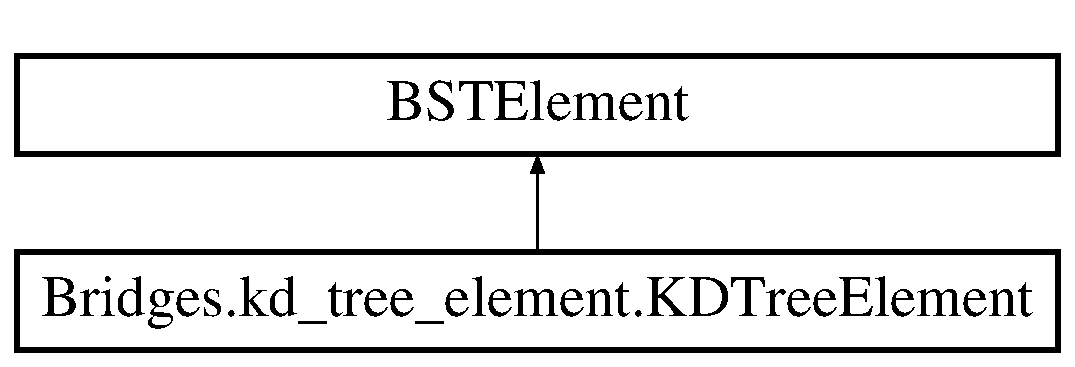
\includegraphics[height=2.000000cm]{class_bridges_1_1kd__tree__element_1_1_k_d_tree_element}
\end{center}
\end{figure}
\subsection*{Public Member Functions}
\begin{DoxyCompactItemize}
\item 
def \hyperlink{class_bridges_1_1kd__tree__element_1_1_k_d_tree_element_ada272bbaead31a3479c54fbbfa1ff467}{\+\_\+\+\_\+init\+\_\+\+\_\+}
\begin{DoxyCompactList}\small\item\em Constructs a Kd\+Tree\+Element wit the provided value, label, key, left and right Kd\+Tree elements. \end{DoxyCompactList}\item 
def \hyperlink{class_bridges_1_1kd__tree__element_1_1_k_d_tree_element_a2a835a57fdbcbad9f24f49421756b923}{get\+\_\+data\+\_\+structure\+\_\+type} (self)
\item 
def \hyperlink{class_bridges_1_1kd__tree__element_1_1_k_d_tree_element_a4ef9a82d8bb407f7e802fad23f0406ab}{get\+\_\+dimension} (self)
\item 
def \hyperlink{class_bridges_1_1kd__tree__element_1_1_k_d_tree_element_ae2c2dc60e110fbe64edd0e9b4a55094f}{set\+\_\+dimension} (self, dim)
\item 
def \hyperlink{class_bridges_1_1kd__tree__element_1_1_k_d_tree_element_a5148bf0c4272f62d7c055ebf2a6a6ede}{get\+\_\+thickness} (self)
\item 
def \hyperlink{class_bridges_1_1kd__tree__element_1_1_k_d_tree_element_ac100a47f4743452747c002dfda86e2b7}{set\+\_\+thickness} (self, th)
\item 
def \hyperlink{class_bridges_1_1kd__tree__element_1_1_k_d_tree_element_a0190cbbb6e52833d711be493af5bb2aa}{get\+\_\+left} (self)
\item 
def \hyperlink{class_bridges_1_1kd__tree__element_1_1_k_d_tree_element_ac02fbf728853a590d59e042110b9ce29}{get\+\_\+right} (self)
\end{DoxyCompactItemize}
\subsection*{Public Attributes}
\begin{DoxyCompactItemize}
\item 
\hyperlink{class_bridges_1_1kd__tree__element_1_1_k_d_tree_element_a530b78c2dcb601a9345b195c1b882d30}{thickness}
\item 
\hyperlink{class_bridges_1_1kd__tree__element_1_1_k_d_tree_element_ab5457d652eacbce763c8760b512ac7d7}{dimension}
\end{DoxyCompactItemize}


\subsection{Detailed Description}
The This class can be used to create K-\/d Tree elements, derived from B\+S\+T\+Element. 

K-\/\+D trees can be thought of as the spatial equivalent binary search trees and operate on multiple dimensions (2\+D and 3\+D are most common). These trees serve as a representation of the underlying geometrically defined spaces. Specialized versions of these trees include quadtrees and octrees, which subdivide into equal sized quadrants octants at each level, respectively. This class extends the B\+S\+T\+Element class by adding a dimension property. It also includes a thickness property for displaying the partitioning lines generated by the convex decomposition.

convenient to generate visual representation to allow for use in a binary search tree implementation.

\begin{DoxyAuthor}{Author}
Kalpathi Subramanian 
\end{DoxyAuthor}
\begin{DoxyDate}{Date}
12/26/18 
\end{DoxyDate}


\subsection{Constructor \& Destructor Documentation}
\hypertarget{class_bridges_1_1kd__tree__element_1_1_k_d_tree_element_ada272bbaead31a3479c54fbbfa1ff467}{}\index{Bridges\+::kd\+\_\+tree\+\_\+element\+::\+K\+D\+Tree\+Element@{Bridges\+::kd\+\_\+tree\+\_\+element\+::\+K\+D\+Tree\+Element}!\+\_\+\+\_\+init\+\_\+\+\_\+@{\+\_\+\+\_\+init\+\_\+\+\_\+}}
\index{\+\_\+\+\_\+init\+\_\+\+\_\+@{\+\_\+\+\_\+init\+\_\+\+\_\+}!Bridges\+::kd\+\_\+tree\+\_\+element\+::\+K\+D\+Tree\+Element@{Bridges\+::kd\+\_\+tree\+\_\+element\+::\+K\+D\+Tree\+Element}}
\subsubsection[{\+\_\+\+\_\+init\+\_\+\+\_\+}]{\setlength{\rightskip}{0pt plus 5cm}def Bridges.\+kd\+\_\+tree\+\_\+element.\+K\+D\+Tree\+Element.\+\_\+\+\_\+init\+\_\+\+\_\+ (
\begin{DoxyParamCaption}
\item[{}]{self, }
\item[{}]{key = {\ttfamily None}, }
\item[{}]{dim = {\ttfamily None}, }
\item[{}]{th = {\ttfamily None}, }
\item[{}]{left = {\ttfamily None}, }
\item[{}]{right = {\ttfamily None}, }
\item[{}]{val = {\ttfamily None}, }
\item[{}]{lab = {\ttfamily None}}
\end{DoxyParamCaption}
)}\label{class_bridges_1_1kd__tree__element_1_1_k_d_tree_element_ada272bbaead31a3479c54fbbfa1ff467}


Constructs a Kd\+Tree\+Element wit the provided value, label, key, left and right Kd\+Tree elements. 

The defaults will be used if not provided


\begin{DoxyParams}{Parameters}
{\em key} & The key for the ordering \\
\hline
{\em val} & The Data to hold \\
\hline
{\em lab} & the label to show \\
\hline
{\em left} & The left Kd\+Tree Element \\
\hline
{\em right} & the right Kd\+Tree element \\
\hline
\end{DoxyParams}


\subsection{Member Function Documentation}
\hypertarget{class_bridges_1_1kd__tree__element_1_1_k_d_tree_element_a2a835a57fdbcbad9f24f49421756b923}{}\index{Bridges\+::kd\+\_\+tree\+\_\+element\+::\+K\+D\+Tree\+Element@{Bridges\+::kd\+\_\+tree\+\_\+element\+::\+K\+D\+Tree\+Element}!get\+\_\+data\+\_\+structure\+\_\+type@{get\+\_\+data\+\_\+structure\+\_\+type}}
\index{get\+\_\+data\+\_\+structure\+\_\+type@{get\+\_\+data\+\_\+structure\+\_\+type}!Bridges\+::kd\+\_\+tree\+\_\+element\+::\+K\+D\+Tree\+Element@{Bridges\+::kd\+\_\+tree\+\_\+element\+::\+K\+D\+Tree\+Element}}
\subsubsection[{get\+\_\+data\+\_\+structure\+\_\+type(self)}]{\setlength{\rightskip}{0pt plus 5cm}def Bridges.\+kd\+\_\+tree\+\_\+element.\+K\+D\+Tree\+Element.\+get\+\_\+data\+\_\+structure\+\_\+type (
\begin{DoxyParamCaption}
\item[{}]{self}
\end{DoxyParamCaption}
)}\label{class_bridges_1_1kd__tree__element_1_1_k_d_tree_element_a2a835a57fdbcbad9f24f49421756b923}
\hypertarget{class_bridges_1_1kd__tree__element_1_1_k_d_tree_element_a4ef9a82d8bb407f7e802fad23f0406ab}{}\index{Bridges\+::kd\+\_\+tree\+\_\+element\+::\+K\+D\+Tree\+Element@{Bridges\+::kd\+\_\+tree\+\_\+element\+::\+K\+D\+Tree\+Element}!get\+\_\+dimension@{get\+\_\+dimension}}
\index{get\+\_\+dimension@{get\+\_\+dimension}!Bridges\+::kd\+\_\+tree\+\_\+element\+::\+K\+D\+Tree\+Element@{Bridges\+::kd\+\_\+tree\+\_\+element\+::\+K\+D\+Tree\+Element}}
\subsubsection[{get\+\_\+dimension(self)}]{\setlength{\rightskip}{0pt plus 5cm}def Bridges.\+kd\+\_\+tree\+\_\+element.\+K\+D\+Tree\+Element.\+get\+\_\+dimension (
\begin{DoxyParamCaption}
\item[{}]{self}
\end{DoxyParamCaption}
)}\label{class_bridges_1_1kd__tree__element_1_1_k_d_tree_element_a4ef9a82d8bb407f7e802fad23f0406ab}
\hypertarget{class_bridges_1_1kd__tree__element_1_1_k_d_tree_element_a0190cbbb6e52833d711be493af5bb2aa}{}\index{Bridges\+::kd\+\_\+tree\+\_\+element\+::\+K\+D\+Tree\+Element@{Bridges\+::kd\+\_\+tree\+\_\+element\+::\+K\+D\+Tree\+Element}!get\+\_\+left@{get\+\_\+left}}
\index{get\+\_\+left@{get\+\_\+left}!Bridges\+::kd\+\_\+tree\+\_\+element\+::\+K\+D\+Tree\+Element@{Bridges\+::kd\+\_\+tree\+\_\+element\+::\+K\+D\+Tree\+Element}}
\subsubsection[{get\+\_\+left(self)}]{\setlength{\rightskip}{0pt plus 5cm}def Bridges.\+kd\+\_\+tree\+\_\+element.\+K\+D\+Tree\+Element.\+get\+\_\+left (
\begin{DoxyParamCaption}
\item[{}]{self}
\end{DoxyParamCaption}
)}\label{class_bridges_1_1kd__tree__element_1_1_k_d_tree_element_a0190cbbb6e52833d711be493af5bb2aa}
\hypertarget{class_bridges_1_1kd__tree__element_1_1_k_d_tree_element_ac02fbf728853a590d59e042110b9ce29}{}\index{Bridges\+::kd\+\_\+tree\+\_\+element\+::\+K\+D\+Tree\+Element@{Bridges\+::kd\+\_\+tree\+\_\+element\+::\+K\+D\+Tree\+Element}!get\+\_\+right@{get\+\_\+right}}
\index{get\+\_\+right@{get\+\_\+right}!Bridges\+::kd\+\_\+tree\+\_\+element\+::\+K\+D\+Tree\+Element@{Bridges\+::kd\+\_\+tree\+\_\+element\+::\+K\+D\+Tree\+Element}}
\subsubsection[{get\+\_\+right(self)}]{\setlength{\rightskip}{0pt plus 5cm}def Bridges.\+kd\+\_\+tree\+\_\+element.\+K\+D\+Tree\+Element.\+get\+\_\+right (
\begin{DoxyParamCaption}
\item[{}]{self}
\end{DoxyParamCaption}
)}\label{class_bridges_1_1kd__tree__element_1_1_k_d_tree_element_ac02fbf728853a590d59e042110b9ce29}
\hypertarget{class_bridges_1_1kd__tree__element_1_1_k_d_tree_element_a5148bf0c4272f62d7c055ebf2a6a6ede}{}\index{Bridges\+::kd\+\_\+tree\+\_\+element\+::\+K\+D\+Tree\+Element@{Bridges\+::kd\+\_\+tree\+\_\+element\+::\+K\+D\+Tree\+Element}!get\+\_\+thickness@{get\+\_\+thickness}}
\index{get\+\_\+thickness@{get\+\_\+thickness}!Bridges\+::kd\+\_\+tree\+\_\+element\+::\+K\+D\+Tree\+Element@{Bridges\+::kd\+\_\+tree\+\_\+element\+::\+K\+D\+Tree\+Element}}
\subsubsection[{get\+\_\+thickness(self)}]{\setlength{\rightskip}{0pt plus 5cm}def Bridges.\+kd\+\_\+tree\+\_\+element.\+K\+D\+Tree\+Element.\+get\+\_\+thickness (
\begin{DoxyParamCaption}
\item[{}]{self}
\end{DoxyParamCaption}
)}\label{class_bridges_1_1kd__tree__element_1_1_k_d_tree_element_a5148bf0c4272f62d7c055ebf2a6a6ede}
\hypertarget{class_bridges_1_1kd__tree__element_1_1_k_d_tree_element_ae2c2dc60e110fbe64edd0e9b4a55094f}{}\index{Bridges\+::kd\+\_\+tree\+\_\+element\+::\+K\+D\+Tree\+Element@{Bridges\+::kd\+\_\+tree\+\_\+element\+::\+K\+D\+Tree\+Element}!set\+\_\+dimension@{set\+\_\+dimension}}
\index{set\+\_\+dimension@{set\+\_\+dimension}!Bridges\+::kd\+\_\+tree\+\_\+element\+::\+K\+D\+Tree\+Element@{Bridges\+::kd\+\_\+tree\+\_\+element\+::\+K\+D\+Tree\+Element}}
\subsubsection[{set\+\_\+dimension(self, dim)}]{\setlength{\rightskip}{0pt plus 5cm}def Bridges.\+kd\+\_\+tree\+\_\+element.\+K\+D\+Tree\+Element.\+set\+\_\+dimension (
\begin{DoxyParamCaption}
\item[{}]{self, }
\item[{}]{dim}
\end{DoxyParamCaption}
)}\label{class_bridges_1_1kd__tree__element_1_1_k_d_tree_element_ae2c2dc60e110fbe64edd0e9b4a55094f}
\hypertarget{class_bridges_1_1kd__tree__element_1_1_k_d_tree_element_ac100a47f4743452747c002dfda86e2b7}{}\index{Bridges\+::kd\+\_\+tree\+\_\+element\+::\+K\+D\+Tree\+Element@{Bridges\+::kd\+\_\+tree\+\_\+element\+::\+K\+D\+Tree\+Element}!set\+\_\+thickness@{set\+\_\+thickness}}
\index{set\+\_\+thickness@{set\+\_\+thickness}!Bridges\+::kd\+\_\+tree\+\_\+element\+::\+K\+D\+Tree\+Element@{Bridges\+::kd\+\_\+tree\+\_\+element\+::\+K\+D\+Tree\+Element}}
\subsubsection[{set\+\_\+thickness(self, th)}]{\setlength{\rightskip}{0pt plus 5cm}def Bridges.\+kd\+\_\+tree\+\_\+element.\+K\+D\+Tree\+Element.\+set\+\_\+thickness (
\begin{DoxyParamCaption}
\item[{}]{self, }
\item[{}]{th}
\end{DoxyParamCaption}
)}\label{class_bridges_1_1kd__tree__element_1_1_k_d_tree_element_ac100a47f4743452747c002dfda86e2b7}


\subsection{Member Data Documentation}
\hypertarget{class_bridges_1_1kd__tree__element_1_1_k_d_tree_element_ab5457d652eacbce763c8760b512ac7d7}{}\index{Bridges\+::kd\+\_\+tree\+\_\+element\+::\+K\+D\+Tree\+Element@{Bridges\+::kd\+\_\+tree\+\_\+element\+::\+K\+D\+Tree\+Element}!dimension@{dimension}}
\index{dimension@{dimension}!Bridges\+::kd\+\_\+tree\+\_\+element\+::\+K\+D\+Tree\+Element@{Bridges\+::kd\+\_\+tree\+\_\+element\+::\+K\+D\+Tree\+Element}}
\subsubsection[{dimension}]{\setlength{\rightskip}{0pt plus 5cm}Bridges.\+kd\+\_\+tree\+\_\+element.\+K\+D\+Tree\+Element.\+dimension}\label{class_bridges_1_1kd__tree__element_1_1_k_d_tree_element_ab5457d652eacbce763c8760b512ac7d7}
\hypertarget{class_bridges_1_1kd__tree__element_1_1_k_d_tree_element_a530b78c2dcb601a9345b195c1b882d30}{}\index{Bridges\+::kd\+\_\+tree\+\_\+element\+::\+K\+D\+Tree\+Element@{Bridges\+::kd\+\_\+tree\+\_\+element\+::\+K\+D\+Tree\+Element}!thickness@{thickness}}
\index{thickness@{thickness}!Bridges\+::kd\+\_\+tree\+\_\+element\+::\+K\+D\+Tree\+Element@{Bridges\+::kd\+\_\+tree\+\_\+element\+::\+K\+D\+Tree\+Element}}
\subsubsection[{thickness}]{\setlength{\rightskip}{0pt plus 5cm}Bridges.\+kd\+\_\+tree\+\_\+element.\+K\+D\+Tree\+Element.\+thickness}\label{class_bridges_1_1kd__tree__element_1_1_k_d_tree_element_a530b78c2dcb601a9345b195c1b882d30}


The documentation for this class was generated from the following file\+:\begin{DoxyCompactItemize}
\item 
/\+Users/kalpathi/gr/bridges/client/python/\+Bridges/\hyperlink{kd__tree__element_8py}{kd\+\_\+tree\+\_\+element.\+py}\end{DoxyCompactItemize}

\hypertarget{class_bridges_1_1label_1_1_label}{}\section{Bridges.\+label.\+Label Class Reference}
\label{class_bridges_1_1label_1_1_label}\index{Bridges.\+label.\+Label@{Bridges.\+label.\+Label}}
Inheritance diagram for Bridges.\+label.\+Label\+:\begin{figure}[H]
\begin{center}
\leavevmode
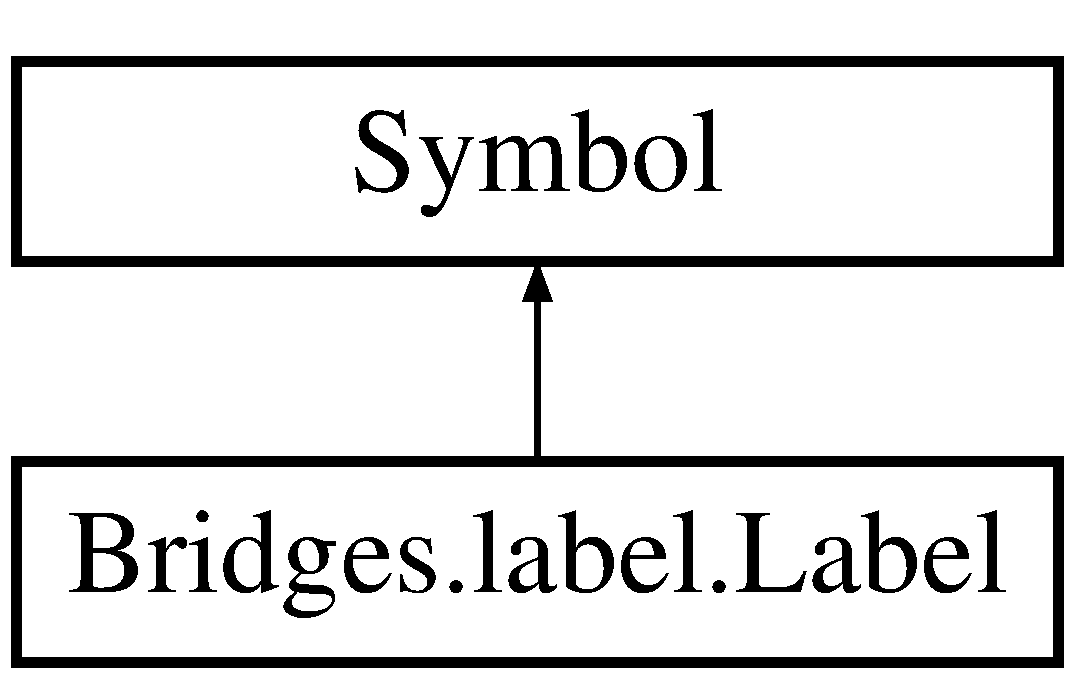
\includegraphics[height=2.000000cm]{class_bridges_1_1label_1_1_label}
\end{center}
\end{figure}
\subsection*{Public Member Functions}
\begin{DoxyCompactItemize}
\item 
def \mbox{\hyperlink{class_bridges_1_1label_1_1_label_a205d9bf35a670f9c3fc91dab4fd4c107}{\+\_\+\+\_\+init\+\_\+\+\_\+}} (self, label=None)
\item 
def \mbox{\hyperlink{class_bridges_1_1label_1_1_label_aff0f1dc269d7c98c77664d3ed9664001}{set\+\_\+font\+\_\+size}} (self, size)
\item 
def \mbox{\hyperlink{class_bridges_1_1label_1_1_label_a05a2618dc5e2350214fcacd5f210dcbc}{get\+\_\+dimensions}} (self)
\item 
def \mbox{\hyperlink{class_bridges_1_1label_1_1_label_a84b96a49d92ddc7ea0b387c37a6fadaf}{get\+\_\+json\+\_\+representation}} (self)
\end{DoxyCompactItemize}
\subsection*{Public Attributes}
\begin{DoxyCompactItemize}
\item 
\mbox{\hyperlink{class_bridges_1_1label_1_1_label_a47c8f760dbd7b2a2e5dc3b94bc9d9ce2}{width}}
\item 
\mbox{\hyperlink{class_bridges_1_1label_1_1_label_a99fa1d9cff754c373fac09b24427df49}{height}}
\item 
\mbox{\hyperlink{class_bridges_1_1label_1_1_label_a1e2e6070c858b66a3f97e7aa91a4ea66}{font\+\_\+size}}
\end{DoxyCompactItemize}


\subsection{Constructor \& Destructor Documentation}
\mbox{\Hypertarget{class_bridges_1_1label_1_1_label_a205d9bf35a670f9c3fc91dab4fd4c107}\label{class_bridges_1_1label_1_1_label_a205d9bf35a670f9c3fc91dab4fd4c107}} 
\index{Bridges\+::label\+::\+Label@{Bridges\+::label\+::\+Label}!\+\_\+\+\_\+init\+\_\+\+\_\+@{\+\_\+\+\_\+init\+\_\+\+\_\+}}
\index{\+\_\+\+\_\+init\+\_\+\+\_\+@{\+\_\+\+\_\+init\+\_\+\+\_\+}!Bridges\+::label\+::\+Label@{Bridges\+::label\+::\+Label}}
\subsubsection{\texorpdfstring{\+\_\+\+\_\+init\+\_\+\+\_\+()}{\_\_init\_\_()}}
{\footnotesize\ttfamily def Bridges.\+label.\+Label.\+\_\+\+\_\+init\+\_\+\+\_\+ (\begin{DoxyParamCaption}\item[{}]{self,  }\item[{}]{label = {\ttfamily None} }\end{DoxyParamCaption})}



\subsection{Member Function Documentation}
\mbox{\Hypertarget{class_bridges_1_1label_1_1_label_a05a2618dc5e2350214fcacd5f210dcbc}\label{class_bridges_1_1label_1_1_label_a05a2618dc5e2350214fcacd5f210dcbc}} 
\index{Bridges\+::label\+::\+Label@{Bridges\+::label\+::\+Label}!get\+\_\+dimensions@{get\+\_\+dimensions}}
\index{get\+\_\+dimensions@{get\+\_\+dimensions}!Bridges\+::label\+::\+Label@{Bridges\+::label\+::\+Label}}
\subsubsection{\texorpdfstring{get\+\_\+dimensions()}{get\_dimensions()}}
{\footnotesize\ttfamily def Bridges.\+label.\+Label.\+get\+\_\+dimensions (\begin{DoxyParamCaption}\item[{}]{self }\end{DoxyParamCaption})}

\mbox{\Hypertarget{class_bridges_1_1label_1_1_label_a84b96a49d92ddc7ea0b387c37a6fadaf}\label{class_bridges_1_1label_1_1_label_a84b96a49d92ddc7ea0b387c37a6fadaf}} 
\index{Bridges\+::label\+::\+Label@{Bridges\+::label\+::\+Label}!get\+\_\+json\+\_\+representation@{get\+\_\+json\+\_\+representation}}
\index{get\+\_\+json\+\_\+representation@{get\+\_\+json\+\_\+representation}!Bridges\+::label\+::\+Label@{Bridges\+::label\+::\+Label}}
\subsubsection{\texorpdfstring{get\+\_\+json\+\_\+representation()}{get\_json\_representation()}}
{\footnotesize\ttfamily def Bridges.\+label.\+Label.\+get\+\_\+json\+\_\+representation (\begin{DoxyParamCaption}\item[{}]{self }\end{DoxyParamCaption})}

\mbox{\Hypertarget{class_bridges_1_1label_1_1_label_aff0f1dc269d7c98c77664d3ed9664001}\label{class_bridges_1_1label_1_1_label_aff0f1dc269d7c98c77664d3ed9664001}} 
\index{Bridges\+::label\+::\+Label@{Bridges\+::label\+::\+Label}!set\+\_\+font\+\_\+size@{set\+\_\+font\+\_\+size}}
\index{set\+\_\+font\+\_\+size@{set\+\_\+font\+\_\+size}!Bridges\+::label\+::\+Label@{Bridges\+::label\+::\+Label}}
\subsubsection{\texorpdfstring{set\+\_\+font\+\_\+size()}{set\_font\_size()}}
{\footnotesize\ttfamily def Bridges.\+label.\+Label.\+set\+\_\+font\+\_\+size (\begin{DoxyParamCaption}\item[{}]{self,  }\item[{}]{size }\end{DoxyParamCaption})}



\subsection{Member Data Documentation}
\mbox{\Hypertarget{class_bridges_1_1label_1_1_label_a1e2e6070c858b66a3f97e7aa91a4ea66}\label{class_bridges_1_1label_1_1_label_a1e2e6070c858b66a3f97e7aa91a4ea66}} 
\index{Bridges\+::label\+::\+Label@{Bridges\+::label\+::\+Label}!font\+\_\+size@{font\+\_\+size}}
\index{font\+\_\+size@{font\+\_\+size}!Bridges\+::label\+::\+Label@{Bridges\+::label\+::\+Label}}
\subsubsection{\texorpdfstring{font\+\_\+size}{font\_size}}
{\footnotesize\ttfamily Bridges.\+label.\+Label.\+font\+\_\+size}

\mbox{\Hypertarget{class_bridges_1_1label_1_1_label_a99fa1d9cff754c373fac09b24427df49}\label{class_bridges_1_1label_1_1_label_a99fa1d9cff754c373fac09b24427df49}} 
\index{Bridges\+::label\+::\+Label@{Bridges\+::label\+::\+Label}!height@{height}}
\index{height@{height}!Bridges\+::label\+::\+Label@{Bridges\+::label\+::\+Label}}
\subsubsection{\texorpdfstring{height}{height}}
{\footnotesize\ttfamily Bridges.\+label.\+Label.\+height}

\mbox{\Hypertarget{class_bridges_1_1label_1_1_label_a47c8f760dbd7b2a2e5dc3b94bc9d9ce2}\label{class_bridges_1_1label_1_1_label_a47c8f760dbd7b2a2e5dc3b94bc9d9ce2}} 
\index{Bridges\+::label\+::\+Label@{Bridges\+::label\+::\+Label}!width@{width}}
\index{width@{width}!Bridges\+::label\+::\+Label@{Bridges\+::label\+::\+Label}}
\subsubsection{\texorpdfstring{width}{width}}
{\footnotesize\ttfamily Bridges.\+label.\+Label.\+width}



The documentation for this class was generated from the following file\+:\begin{DoxyCompactItemize}
\item 
/\+Users/kalpathi/gr/bridges/client/python/bridges18/\+Bridges/\mbox{\hyperlink{label_8py}{label.\+py}}\end{DoxyCompactItemize}

\hypertarget{class_bridges_1_1link__visualizer_1_1_link_visualizer}{}\section{Bridges.\+link\+\_\+visualizer.\+Link\+Visualizer Class Reference}
\label{class_bridges_1_1link__visualizer_1_1_link_visualizer}\index{Bridges.\+link\+\_\+visualizer.\+Link\+Visualizer@{Bridges.\+link\+\_\+visualizer.\+Link\+Visualizer}}


This class maintains the visual attributes of links that join bridges elements.  


Inheritance diagram for Bridges.\+link\+\_\+visualizer.\+Link\+Visualizer\+:\begin{figure}[H]
\begin{center}
\leavevmode
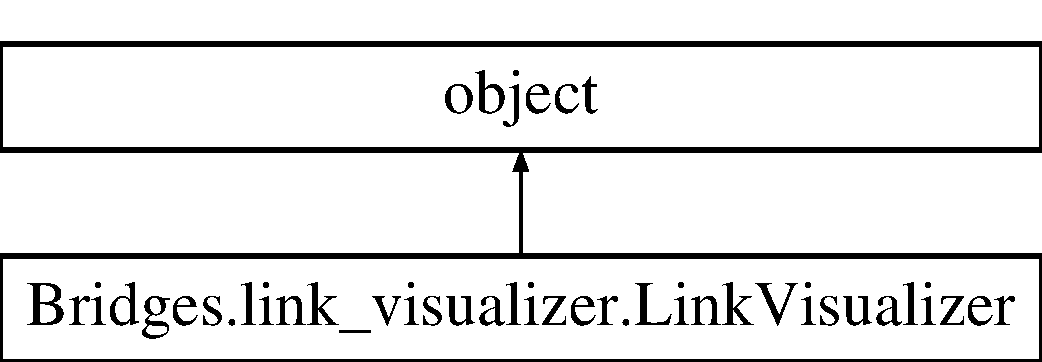
\includegraphics[height=2.000000cm]{class_bridges_1_1link__visualizer_1_1_link_visualizer}
\end{center}
\end{figure}
\subsection*{Public Member Functions}
\begin{DoxyCompactItemize}
\item 
def \mbox{\hyperlink{class_bridges_1_1link__visualizer_1_1_link_visualizer_abeac165689bb892581a9cf379a8e4c3f}{\+\_\+\+\_\+init\+\_\+\+\_\+}} (self)
\item 
def \mbox{\hyperlink{class_bridges_1_1link__visualizer_1_1_link_visualizer_ad29bf7c34d1cfc37e57f98cd539d6a71}{set\+\_\+thickness}} (self, th)
\begin{DoxyCompactList}\small\item\em Set the thickness of the link in the Bridge Visualization in pixels; thickness shoudl be in the range 0-\/50.\+0. \end{DoxyCompactList}\item 
def \mbox{\hyperlink{class_bridges_1_1link__visualizer_1_1_link_visualizer_a4e244bf5161201be4401abcc55af7b59}{get\+\_\+thickness}} (self)
\begin{DoxyCompactList}\small\item\em Get the thickness of the link in the bridges Visualiation. \end{DoxyCompactList}\item 
def \mbox{\hyperlink{class_bridges_1_1link__visualizer_1_1_link_visualizer_ae439433344182c699ba4363e47de3949}{set\+\_\+weight}} (self, wt)
\begin{DoxyCompactList}\small\item\em Set the weight of the link, useful in graph algorithms, for example. \end{DoxyCompactList}\item 
def \mbox{\hyperlink{class_bridges_1_1link__visualizer_1_1_link_visualizer_a90d526570f2c6cc485c465fe7ffc6ecf}{get\+\_\+weight}} (self)
\begin{DoxyCompactList}\small\item\em Get the weight of the link. \end{DoxyCompactList}\item 
def \mbox{\hyperlink{class_bridges_1_1link__visualizer_1_1_link_visualizer_a73841d196425d4688aba60226e891da5}{set\+\_\+color}} (self, args, kwargs)
\begin{DoxyCompactList}\small\item\em Set the color of the link in the bridges Visualization to \char`\"{}a\+Color\char`\"{}. \end{DoxyCompactList}\item 
def \mbox{\hyperlink{class_bridges_1_1link__visualizer_1_1_link_visualizer_af3b061f20b383565b99b9b80d4901a60}{get\+\_\+color}} (self)
\begin{DoxyCompactList}\small\item\em Get the color of the link in the bridges Visualization. \end{DoxyCompactList}\item 
def \mbox{\hyperlink{class_bridges_1_1link__visualizer_1_1_link_visualizer_a46cb7057831aba1a5cd25d49552629e5}{set\+\_\+opacity}} (self, opacity)
\begin{DoxyCompactList}\small\item\em Sets the opacity of the link in the bridges Visualization. \end{DoxyCompactList}\item 
def \mbox{\hyperlink{class_bridges_1_1link__visualizer_1_1_link_visualizer_ad9623595bcbe1da3a19368a89d3bc7cb}{get\+\_\+opacity}} (self)
\begin{DoxyCompactList}\small\item\em Get the opacity of the link in the bridges Visualization. \end{DoxyCompactList}\item 
def \mbox{\hyperlink{class_bridges_1_1link__visualizer_1_1_link_visualizer_a3ea7e9b8eda72169ca2819a84cb5faa7}{get\+\_\+link\+\_\+properties}} (self)
\end{DoxyCompactItemize}
\subsection*{Public Attributes}
\begin{DoxyCompactItemize}
\item 
\mbox{\hyperlink{class_bridges_1_1link__visualizer_1_1_link_visualizer_a66caf26ee75f2f33f650e76a40c72488}{color}}
\end{DoxyCompactItemize}
\subsection*{Static Public Attributes}
\begin{DoxyCompactItemize}
\item 
string \mbox{\hyperlink{class_bridges_1_1link__visualizer_1_1_link_visualizer_a46d14fbb36b1bc7a49803efe3ece1f23}{Q\+U\+O\+TE}} = \char`\"{}\textbackslash{}\char`\"{}\char`\"{}
\item 
string \mbox{\hyperlink{class_bridges_1_1link__visualizer_1_1_link_visualizer_a94ebac44734dfdd10964d2fc3d8f623a}{C\+O\+M\+MA}} = \char`\"{},\char`\"{}
\item 
string \mbox{\hyperlink{class_bridges_1_1link__visualizer_1_1_link_visualizer_ae2e8741c1e2d35554350c33e4feab0f4}{C\+O\+L\+ON}} = \char`\"{}\+:\char`\"{}
\item 
string \mbox{\hyperlink{class_bridges_1_1link__visualizer_1_1_link_visualizer_a3fccd1dbd36b6e1e6a4280196c0cda33}{O\+P\+E\+N\+\_\+\+C\+U\+R\+LY}} = \char`\"{}\{\char`\"{}
\item 
string \mbox{\hyperlink{class_bridges_1_1link__visualizer_1_1_link_visualizer_a29483e4a583457637b9aa0e215849fee}{C\+L\+O\+S\+E\+\_\+\+C\+U\+R\+LY}} = \char`\"{}\}\char`\"{}
\item 
string \mbox{\hyperlink{class_bridges_1_1link__visualizer_1_1_link_visualizer_ac0955586c3a02eff91be97724bcfbea0}{O\+P\+E\+N\+\_\+\+P\+A\+R\+EN}} = \char`\"{}(\char`\"{}
\item 
string \mbox{\hyperlink{class_bridges_1_1link__visualizer_1_1_link_visualizer_a71fd9eda5358b12793bbe9ca74cbc640}{C\+L\+O\+S\+E\+\_\+\+P\+A\+R\+EN}} = \char`\"{})\char`\"{}
\item 
string \mbox{\hyperlink{class_bridges_1_1link__visualizer_1_1_link_visualizer_a0b0c770c7e5f05774c376882619396e1}{O\+P\+E\+N\+\_\+\+B\+OX}} = \char`\"{}\mbox{[}\char`\"{}
\item 
string \mbox{\hyperlink{class_bridges_1_1link__visualizer_1_1_link_visualizer_a3cb1f0ee010a5173373a38a729164461}{C\+L\+O\+S\+E\+\_\+\+B\+OX}} = \char`\"{}\mbox{]}\char`\"{}
\item 
\mbox{\hyperlink{class_bridges_1_1link__visualizer_1_1_link_visualizer_acbc2abcd8584b20c14f3aa695cb5a668}{thickness}} = float()
\item 
\mbox{\hyperlink{class_bridges_1_1link__visualizer_1_1_link_visualizer_a3cf821801816ca20db68e8122b159e96}{weight}} = float()
\end{DoxyCompactItemize}


\subsection{Detailed Description}
This class maintains the visual attributes of links that join bridges elements. 

Visual properties include color, thickness, and opacity. Objects of this class are stored as part of the Element class. Generally, a user will manipulate the \mbox{\hyperlink{class_bridges_1_1link__visualizer_1_1_link_visualizer}{Link\+Visualizer}} returned from the Element\textquotesingle{}s get\+Link\+Visualizer(\+Element it) method (which it is the bridges element this element is linked to), and then set attributes using its methods. Links are utilized in all types of linked lists, tree and graph structures.

Supported attribute values are as follows\+:

{\bfseries Supported Colors (by name)}\+: 

\char`\"{}red\char`\"{}, \char`\"{}green\char`\"{}, \char`\"{}blue\char`\"{},\char`\"{}yellow\char`\"{},\char`\"{}cyan\char`\"{},\char`\"{}magenta\char`\"{}, \char`\"{}white\char`\"{},, \char`\"{}black\char`\"{}, \char`\"{}orange\char`\"{}, \char`\"{}turquoise\char`\"{}, \char`\"{}maroon\char`\"{}, ~\newline
 \char`\"{}aquamarine\char`\"{}, \char`\"{}azure\char`\"{}, \char`\"{}beige\char`\"{}, \char`\"{}brown\char`\"{}, \char`\"{}tan\char`\"{}, \char`\"{}olive\char`\"{}, \char`\"{}chartreuse\char`\"{}, \char`\"{}khaki\char`\"{}, \char`\"{}bisque\char`\"{}, \char`\"{}coral\char`\"{}, ~\newline
 \char`\"{}pink\char`\"{}, \char`\"{}lavender\char`\"{}, \char`\"{}purple\char`\"{}, \char`\"{}gold\char`\"{} 

{\bfseries  Color by R\+G\+BA Specification \+:} Range\+: 0-\/255 for each component 

{\bfseries  Thickness\+: } Range \+: 0.\+0-\/50.\+0

{\bfseries  Opacity\+: } Range (0.\+0-\/1.\+0) 

\begin{DoxyAuthor}{Author}
Mihai Mehedint, Kalpathi Subramanian
\end{DoxyAuthor}
\begin{DoxySeeAlso}{See also}
Example Tutorial at ~\newline
 \href{http://bridgesuncc.github.io/Hello_World_Tutorials/SLL.html}{\tt http\+://bridgesuncc.\+github.\+io/\+Hello\+\_\+\+World\+\_\+\+Tutorials/\+S\+L\+L.\+html} 
\end{DoxySeeAlso}


\subsection{Constructor \& Destructor Documentation}
\mbox{\Hypertarget{class_bridges_1_1link__visualizer_1_1_link_visualizer_abeac165689bb892581a9cf379a8e4c3f}\label{class_bridges_1_1link__visualizer_1_1_link_visualizer_abeac165689bb892581a9cf379a8e4c3f}} 
\index{Bridges\+::link\+\_\+visualizer\+::\+Link\+Visualizer@{Bridges\+::link\+\_\+visualizer\+::\+Link\+Visualizer}!\+\_\+\+\_\+init\+\_\+\+\_\+@{\+\_\+\+\_\+init\+\_\+\+\_\+}}
\index{\+\_\+\+\_\+init\+\_\+\+\_\+@{\+\_\+\+\_\+init\+\_\+\+\_\+}!Bridges\+::link\+\_\+visualizer\+::\+Link\+Visualizer@{Bridges\+::link\+\_\+visualizer\+::\+Link\+Visualizer}}
\subsubsection{\texorpdfstring{\+\_\+\+\_\+init\+\_\+\+\_\+()}{\_\_init\_\_()}}
{\footnotesize\ttfamily def Bridges.\+link\+\_\+visualizer.\+Link\+Visualizer.\+\_\+\+\_\+init\+\_\+\+\_\+ (\begin{DoxyParamCaption}\item[{}]{self }\end{DoxyParamCaption})}



\subsection{Member Function Documentation}
\mbox{\Hypertarget{class_bridges_1_1link__visualizer_1_1_link_visualizer_af3b061f20b383565b99b9b80d4901a60}\label{class_bridges_1_1link__visualizer_1_1_link_visualizer_af3b061f20b383565b99b9b80d4901a60}} 
\index{Bridges\+::link\+\_\+visualizer\+::\+Link\+Visualizer@{Bridges\+::link\+\_\+visualizer\+::\+Link\+Visualizer}!get\+\_\+color@{get\+\_\+color}}
\index{get\+\_\+color@{get\+\_\+color}!Bridges\+::link\+\_\+visualizer\+::\+Link\+Visualizer@{Bridges\+::link\+\_\+visualizer\+::\+Link\+Visualizer}}
\subsubsection{\texorpdfstring{get\+\_\+color()}{get\_color()}}
{\footnotesize\ttfamily def Bridges.\+link\+\_\+visualizer.\+Link\+Visualizer.\+get\+\_\+color (\begin{DoxyParamCaption}\item[{}]{self }\end{DoxyParamCaption})}



Get the color of the link in the bridges Visualization. 

\begin{DoxyReturn}{Returns}
the Color object representing the color of the link 
\end{DoxyReturn}
\mbox{\Hypertarget{class_bridges_1_1link__visualizer_1_1_link_visualizer_a3ea7e9b8eda72169ca2819a84cb5faa7}\label{class_bridges_1_1link__visualizer_1_1_link_visualizer_a3ea7e9b8eda72169ca2819a84cb5faa7}} 
\index{Bridges\+::link\+\_\+visualizer\+::\+Link\+Visualizer@{Bridges\+::link\+\_\+visualizer\+::\+Link\+Visualizer}!get\+\_\+link\+\_\+properties@{get\+\_\+link\+\_\+properties}}
\index{get\+\_\+link\+\_\+properties@{get\+\_\+link\+\_\+properties}!Bridges\+::link\+\_\+visualizer\+::\+Link\+Visualizer@{Bridges\+::link\+\_\+visualizer\+::\+Link\+Visualizer}}
\subsubsection{\texorpdfstring{get\+\_\+link\+\_\+properties()}{get\_link\_properties()}}
{\footnotesize\ttfamily def Bridges.\+link\+\_\+visualizer.\+Link\+Visualizer.\+get\+\_\+link\+\_\+properties (\begin{DoxyParamCaption}\item[{}]{self }\end{DoxyParamCaption})}

\mbox{\Hypertarget{class_bridges_1_1link__visualizer_1_1_link_visualizer_ad9623595bcbe1da3a19368a89d3bc7cb}\label{class_bridges_1_1link__visualizer_1_1_link_visualizer_ad9623595bcbe1da3a19368a89d3bc7cb}} 
\index{Bridges\+::link\+\_\+visualizer\+::\+Link\+Visualizer@{Bridges\+::link\+\_\+visualizer\+::\+Link\+Visualizer}!get\+\_\+opacity@{get\+\_\+opacity}}
\index{get\+\_\+opacity@{get\+\_\+opacity}!Bridges\+::link\+\_\+visualizer\+::\+Link\+Visualizer@{Bridges\+::link\+\_\+visualizer\+::\+Link\+Visualizer}}
\subsubsection{\texorpdfstring{get\+\_\+opacity()}{get\_opacity()}}
{\footnotesize\ttfamily def Bridges.\+link\+\_\+visualizer.\+Link\+Visualizer.\+get\+\_\+opacity (\begin{DoxyParamCaption}\item[{}]{self }\end{DoxyParamCaption})}



Get the opacity of the link in the bridges Visualization. 

\begin{DoxyReturn}{Returns}
the opacity value (in the range 0.\+0-\/1.\+0 
\end{DoxyReturn}
\mbox{\Hypertarget{class_bridges_1_1link__visualizer_1_1_link_visualizer_a4e244bf5161201be4401abcc55af7b59}\label{class_bridges_1_1link__visualizer_1_1_link_visualizer_a4e244bf5161201be4401abcc55af7b59}} 
\index{Bridges\+::link\+\_\+visualizer\+::\+Link\+Visualizer@{Bridges\+::link\+\_\+visualizer\+::\+Link\+Visualizer}!get\+\_\+thickness@{get\+\_\+thickness}}
\index{get\+\_\+thickness@{get\+\_\+thickness}!Bridges\+::link\+\_\+visualizer\+::\+Link\+Visualizer@{Bridges\+::link\+\_\+visualizer\+::\+Link\+Visualizer}}
\subsubsection{\texorpdfstring{get\+\_\+thickness()}{get\_thickness()}}
{\footnotesize\ttfamily def Bridges.\+link\+\_\+visualizer.\+Link\+Visualizer.\+get\+\_\+thickness (\begin{DoxyParamCaption}\item[{}]{self }\end{DoxyParamCaption})}



Get the thickness of the link in the bridges Visualiation. 

\begin{DoxyReturn}{Returns}
the size in pixels of the Element in the bridges Visualization 
\end{DoxyReturn}
\mbox{\Hypertarget{class_bridges_1_1link__visualizer_1_1_link_visualizer_a90d526570f2c6cc485c465fe7ffc6ecf}\label{class_bridges_1_1link__visualizer_1_1_link_visualizer_a90d526570f2c6cc485c465fe7ffc6ecf}} 
\index{Bridges\+::link\+\_\+visualizer\+::\+Link\+Visualizer@{Bridges\+::link\+\_\+visualizer\+::\+Link\+Visualizer}!get\+\_\+weight@{get\+\_\+weight}}
\index{get\+\_\+weight@{get\+\_\+weight}!Bridges\+::link\+\_\+visualizer\+::\+Link\+Visualizer@{Bridges\+::link\+\_\+visualizer\+::\+Link\+Visualizer}}
\subsubsection{\texorpdfstring{get\+\_\+weight()}{get\_weight()}}
{\footnotesize\ttfamily def Bridges.\+link\+\_\+visualizer.\+Link\+Visualizer.\+get\+\_\+weight (\begin{DoxyParamCaption}\item[{}]{self }\end{DoxyParamCaption})}



Get the weight of the link. 

\begin{DoxyReturn}{Returns}
the stored edge weight 
\end{DoxyReturn}
\mbox{\Hypertarget{class_bridges_1_1link__visualizer_1_1_link_visualizer_a73841d196425d4688aba60226e891da5}\label{class_bridges_1_1link__visualizer_1_1_link_visualizer_a73841d196425d4688aba60226e891da5}} 
\index{Bridges\+::link\+\_\+visualizer\+::\+Link\+Visualizer@{Bridges\+::link\+\_\+visualizer\+::\+Link\+Visualizer}!set\+\_\+color@{set\+\_\+color}}
\index{set\+\_\+color@{set\+\_\+color}!Bridges\+::link\+\_\+visualizer\+::\+Link\+Visualizer@{Bridges\+::link\+\_\+visualizer\+::\+Link\+Visualizer}}
\subsubsection{\texorpdfstring{set\+\_\+color()}{set\_color()}}
{\footnotesize\ttfamily def Bridges.\+link\+\_\+visualizer.\+Link\+Visualizer.\+set\+\_\+color (\begin{DoxyParamCaption}\item[{}]{self,  }\item[{}]{args,  }\item[{}]{kwargs }\end{DoxyParamCaption})}



Set the color of the link in the bridges Visualization to \char`\"{}a\+Color\char`\"{}. 


\begin{DoxyParams}{Parameters}
{\em col\+\_\+name} & the string reprsenting the color of the Element in the bridges Visualization; supported named colors are \char`\"{}red\char`\"{}, \char`\"{}green\char`\"{}, \char`\"{}blue\char`\"{}, \char`\"{}yellow\char`\"{}, \char`\"{}cyan\char`\"{}, \char`\"{}magenta\char`\"{}, \char`\"{}white\char`\"{}, \char`\"{}black\char`\"{}, \char`\"{}orange\char`\"{}, \char`\"{}turquoise\char`\"{}, \char`\"{}maroon\char`\"{}, \char`\"{}aquamarine\char`\"{}, \char`\"{}azure\char`\"{}, \char`\"{}beige\char`\"{}, \char`\"{}brown\char`\"{}, \char`\"{}tan\char`\"{}, \char`\"{}olive\char`\"{}, \char`\"{}chartreuse\char`\"{}, \char`\"{}khaki\char`\"{}, \char`\"{}bisque\char`\"{}, \char`\"{}coral\char`\"{}, \char`\"{}pink\char`\"{}, \char`\"{}lavender\char`\"{}, \char`\"{}purple\char`\"{}, \char`\"{}gold\char`\"{}\begin{DoxyVerb}Usage: requires either 3 ints 0-255 for RGB and an optional float 0.0-1.0 for alpha or a str of a web color
can also key the RGBA values with r, g, b, a or red, green, blue, alpha respectively and col_name for the str
:param args: int, int, int optional float or str
:param kwargs: r/red: int, b/blue: int, g/green: int optional a/alpha: float or col_name: str
:return: None
\end{DoxyVerb}
 \\
\hline
\end{DoxyParams}
\mbox{\Hypertarget{class_bridges_1_1link__visualizer_1_1_link_visualizer_a46cb7057831aba1a5cd25d49552629e5}\label{class_bridges_1_1link__visualizer_1_1_link_visualizer_a46cb7057831aba1a5cd25d49552629e5}} 
\index{Bridges\+::link\+\_\+visualizer\+::\+Link\+Visualizer@{Bridges\+::link\+\_\+visualizer\+::\+Link\+Visualizer}!set\+\_\+opacity@{set\+\_\+opacity}}
\index{set\+\_\+opacity@{set\+\_\+opacity}!Bridges\+::link\+\_\+visualizer\+::\+Link\+Visualizer@{Bridges\+::link\+\_\+visualizer\+::\+Link\+Visualizer}}
\subsubsection{\texorpdfstring{set\+\_\+opacity()}{set\_opacity()}}
{\footnotesize\ttfamily def Bridges.\+link\+\_\+visualizer.\+Link\+Visualizer.\+set\+\_\+opacity (\begin{DoxyParamCaption}\item[{}]{self,  }\item[{}]{opacity }\end{DoxyParamCaption})}



Sets the opacity of the link in the bridges Visualization. 


\begin{DoxyParams}{Parameters}
{\em opacity} & a float between 0 and 1 representing how transparent the node should be on the bridges Visualization. 0 for invisible, 1 for fully visible, a decimal between 0 and 1 for varying transparency. \\
\hline
\end{DoxyParams}
\mbox{\Hypertarget{class_bridges_1_1link__visualizer_1_1_link_visualizer_ad29bf7c34d1cfc37e57f98cd539d6a71}\label{class_bridges_1_1link__visualizer_1_1_link_visualizer_ad29bf7c34d1cfc37e57f98cd539d6a71}} 
\index{Bridges\+::link\+\_\+visualizer\+::\+Link\+Visualizer@{Bridges\+::link\+\_\+visualizer\+::\+Link\+Visualizer}!set\+\_\+thickness@{set\+\_\+thickness}}
\index{set\+\_\+thickness@{set\+\_\+thickness}!Bridges\+::link\+\_\+visualizer\+::\+Link\+Visualizer@{Bridges\+::link\+\_\+visualizer\+::\+Link\+Visualizer}}
\subsubsection{\texorpdfstring{set\+\_\+thickness()}{set\_thickness()}}
{\footnotesize\ttfamily def Bridges.\+link\+\_\+visualizer.\+Link\+Visualizer.\+set\+\_\+thickness (\begin{DoxyParamCaption}\item[{}]{self,  }\item[{}]{th }\end{DoxyParamCaption})}



Set the thickness of the link in the Bridge Visualization in pixels; thickness shoudl be in the range 0-\/50.\+0. 


\begin{DoxyParams}{Parameters}
{\em thickness} & \\
\hline
\end{DoxyParams}
\mbox{\Hypertarget{class_bridges_1_1link__visualizer_1_1_link_visualizer_ae439433344182c699ba4363e47de3949}\label{class_bridges_1_1link__visualizer_1_1_link_visualizer_ae439433344182c699ba4363e47de3949}} 
\index{Bridges\+::link\+\_\+visualizer\+::\+Link\+Visualizer@{Bridges\+::link\+\_\+visualizer\+::\+Link\+Visualizer}!set\+\_\+weight@{set\+\_\+weight}}
\index{set\+\_\+weight@{set\+\_\+weight}!Bridges\+::link\+\_\+visualizer\+::\+Link\+Visualizer@{Bridges\+::link\+\_\+visualizer\+::\+Link\+Visualizer}}
\subsubsection{\texorpdfstring{set\+\_\+weight()}{set\_weight()}}
{\footnotesize\ttfamily def Bridges.\+link\+\_\+visualizer.\+Link\+Visualizer.\+set\+\_\+weight (\begin{DoxyParamCaption}\item[{}]{self,  }\item[{}]{wt }\end{DoxyParamCaption})}



Set the weight of the link, useful in graph algorithms, for example. 

weight value is user defined, and determined by the input graph specification.


\begin{DoxyParams}{Parameters}
{\em weight} & \\
\hline
\end{DoxyParams}


\subsection{Member Data Documentation}
\mbox{\Hypertarget{class_bridges_1_1link__visualizer_1_1_link_visualizer_a3cb1f0ee010a5173373a38a729164461}\label{class_bridges_1_1link__visualizer_1_1_link_visualizer_a3cb1f0ee010a5173373a38a729164461}} 
\index{Bridges\+::link\+\_\+visualizer\+::\+Link\+Visualizer@{Bridges\+::link\+\_\+visualizer\+::\+Link\+Visualizer}!C\+L\+O\+S\+E\+\_\+\+B\+OX@{C\+L\+O\+S\+E\+\_\+\+B\+OX}}
\index{C\+L\+O\+S\+E\+\_\+\+B\+OX@{C\+L\+O\+S\+E\+\_\+\+B\+OX}!Bridges\+::link\+\_\+visualizer\+::\+Link\+Visualizer@{Bridges\+::link\+\_\+visualizer\+::\+Link\+Visualizer}}
\subsubsection{\texorpdfstring{C\+L\+O\+S\+E\+\_\+\+B\+OX}{CLOSE\_BOX}}
{\footnotesize\ttfamily string Bridges.\+link\+\_\+visualizer.\+Link\+Visualizer.\+C\+L\+O\+S\+E\+\_\+\+B\+OX = \char`\"{}\mbox{]}\char`\"{}\hspace{0.3cm}{\ttfamily [static]}}

\mbox{\Hypertarget{class_bridges_1_1link__visualizer_1_1_link_visualizer_a29483e4a583457637b9aa0e215849fee}\label{class_bridges_1_1link__visualizer_1_1_link_visualizer_a29483e4a583457637b9aa0e215849fee}} 
\index{Bridges\+::link\+\_\+visualizer\+::\+Link\+Visualizer@{Bridges\+::link\+\_\+visualizer\+::\+Link\+Visualizer}!C\+L\+O\+S\+E\+\_\+\+C\+U\+R\+LY@{C\+L\+O\+S\+E\+\_\+\+C\+U\+R\+LY}}
\index{C\+L\+O\+S\+E\+\_\+\+C\+U\+R\+LY@{C\+L\+O\+S\+E\+\_\+\+C\+U\+R\+LY}!Bridges\+::link\+\_\+visualizer\+::\+Link\+Visualizer@{Bridges\+::link\+\_\+visualizer\+::\+Link\+Visualizer}}
\subsubsection{\texorpdfstring{C\+L\+O\+S\+E\+\_\+\+C\+U\+R\+LY}{CLOSE\_CURLY}}
{\footnotesize\ttfamily string Bridges.\+link\+\_\+visualizer.\+Link\+Visualizer.\+C\+L\+O\+S\+E\+\_\+\+C\+U\+R\+LY = \char`\"{}\}\char`\"{}\hspace{0.3cm}{\ttfamily [static]}}

\mbox{\Hypertarget{class_bridges_1_1link__visualizer_1_1_link_visualizer_a71fd9eda5358b12793bbe9ca74cbc640}\label{class_bridges_1_1link__visualizer_1_1_link_visualizer_a71fd9eda5358b12793bbe9ca74cbc640}} 
\index{Bridges\+::link\+\_\+visualizer\+::\+Link\+Visualizer@{Bridges\+::link\+\_\+visualizer\+::\+Link\+Visualizer}!C\+L\+O\+S\+E\+\_\+\+P\+A\+R\+EN@{C\+L\+O\+S\+E\+\_\+\+P\+A\+R\+EN}}
\index{C\+L\+O\+S\+E\+\_\+\+P\+A\+R\+EN@{C\+L\+O\+S\+E\+\_\+\+P\+A\+R\+EN}!Bridges\+::link\+\_\+visualizer\+::\+Link\+Visualizer@{Bridges\+::link\+\_\+visualizer\+::\+Link\+Visualizer}}
\subsubsection{\texorpdfstring{C\+L\+O\+S\+E\+\_\+\+P\+A\+R\+EN}{CLOSE\_PAREN}}
{\footnotesize\ttfamily string Bridges.\+link\+\_\+visualizer.\+Link\+Visualizer.\+C\+L\+O\+S\+E\+\_\+\+P\+A\+R\+EN = \char`\"{})\char`\"{}\hspace{0.3cm}{\ttfamily [static]}}

\mbox{\Hypertarget{class_bridges_1_1link__visualizer_1_1_link_visualizer_ae2e8741c1e2d35554350c33e4feab0f4}\label{class_bridges_1_1link__visualizer_1_1_link_visualizer_ae2e8741c1e2d35554350c33e4feab0f4}} 
\index{Bridges\+::link\+\_\+visualizer\+::\+Link\+Visualizer@{Bridges\+::link\+\_\+visualizer\+::\+Link\+Visualizer}!C\+O\+L\+ON@{C\+O\+L\+ON}}
\index{C\+O\+L\+ON@{C\+O\+L\+ON}!Bridges\+::link\+\_\+visualizer\+::\+Link\+Visualizer@{Bridges\+::link\+\_\+visualizer\+::\+Link\+Visualizer}}
\subsubsection{\texorpdfstring{C\+O\+L\+ON}{COLON}}
{\footnotesize\ttfamily string Bridges.\+link\+\_\+visualizer.\+Link\+Visualizer.\+C\+O\+L\+ON = \char`\"{}\+:\char`\"{}\hspace{0.3cm}{\ttfamily [static]}}

\mbox{\Hypertarget{class_bridges_1_1link__visualizer_1_1_link_visualizer_a66caf26ee75f2f33f650e76a40c72488}\label{class_bridges_1_1link__visualizer_1_1_link_visualizer_a66caf26ee75f2f33f650e76a40c72488}} 
\index{Bridges\+::link\+\_\+visualizer\+::\+Link\+Visualizer@{Bridges\+::link\+\_\+visualizer\+::\+Link\+Visualizer}!color@{color}}
\index{color@{color}!Bridges\+::link\+\_\+visualizer\+::\+Link\+Visualizer@{Bridges\+::link\+\_\+visualizer\+::\+Link\+Visualizer}}
\subsubsection{\texorpdfstring{color}{color}}
{\footnotesize\ttfamily Bridges.\+link\+\_\+visualizer.\+Link\+Visualizer.\+color}

\mbox{\Hypertarget{class_bridges_1_1link__visualizer_1_1_link_visualizer_a94ebac44734dfdd10964d2fc3d8f623a}\label{class_bridges_1_1link__visualizer_1_1_link_visualizer_a94ebac44734dfdd10964d2fc3d8f623a}} 
\index{Bridges\+::link\+\_\+visualizer\+::\+Link\+Visualizer@{Bridges\+::link\+\_\+visualizer\+::\+Link\+Visualizer}!C\+O\+M\+MA@{C\+O\+M\+MA}}
\index{C\+O\+M\+MA@{C\+O\+M\+MA}!Bridges\+::link\+\_\+visualizer\+::\+Link\+Visualizer@{Bridges\+::link\+\_\+visualizer\+::\+Link\+Visualizer}}
\subsubsection{\texorpdfstring{C\+O\+M\+MA}{COMMA}}
{\footnotesize\ttfamily string Bridges.\+link\+\_\+visualizer.\+Link\+Visualizer.\+C\+O\+M\+MA = \char`\"{},\char`\"{}\hspace{0.3cm}{\ttfamily [static]}}

\mbox{\Hypertarget{class_bridges_1_1link__visualizer_1_1_link_visualizer_a0b0c770c7e5f05774c376882619396e1}\label{class_bridges_1_1link__visualizer_1_1_link_visualizer_a0b0c770c7e5f05774c376882619396e1}} 
\index{Bridges\+::link\+\_\+visualizer\+::\+Link\+Visualizer@{Bridges\+::link\+\_\+visualizer\+::\+Link\+Visualizer}!O\+P\+E\+N\+\_\+\+B\+OX@{O\+P\+E\+N\+\_\+\+B\+OX}}
\index{O\+P\+E\+N\+\_\+\+B\+OX@{O\+P\+E\+N\+\_\+\+B\+OX}!Bridges\+::link\+\_\+visualizer\+::\+Link\+Visualizer@{Bridges\+::link\+\_\+visualizer\+::\+Link\+Visualizer}}
\subsubsection{\texorpdfstring{O\+P\+E\+N\+\_\+\+B\+OX}{OPEN\_BOX}}
{\footnotesize\ttfamily string Bridges.\+link\+\_\+visualizer.\+Link\+Visualizer.\+O\+P\+E\+N\+\_\+\+B\+OX = \char`\"{}\mbox{[}\char`\"{}\hspace{0.3cm}{\ttfamily [static]}}

\mbox{\Hypertarget{class_bridges_1_1link__visualizer_1_1_link_visualizer_a3fccd1dbd36b6e1e6a4280196c0cda33}\label{class_bridges_1_1link__visualizer_1_1_link_visualizer_a3fccd1dbd36b6e1e6a4280196c0cda33}} 
\index{Bridges\+::link\+\_\+visualizer\+::\+Link\+Visualizer@{Bridges\+::link\+\_\+visualizer\+::\+Link\+Visualizer}!O\+P\+E\+N\+\_\+\+C\+U\+R\+LY@{O\+P\+E\+N\+\_\+\+C\+U\+R\+LY}}
\index{O\+P\+E\+N\+\_\+\+C\+U\+R\+LY@{O\+P\+E\+N\+\_\+\+C\+U\+R\+LY}!Bridges\+::link\+\_\+visualizer\+::\+Link\+Visualizer@{Bridges\+::link\+\_\+visualizer\+::\+Link\+Visualizer}}
\subsubsection{\texorpdfstring{O\+P\+E\+N\+\_\+\+C\+U\+R\+LY}{OPEN\_CURLY}}
{\footnotesize\ttfamily string Bridges.\+link\+\_\+visualizer.\+Link\+Visualizer.\+O\+P\+E\+N\+\_\+\+C\+U\+R\+LY = \char`\"{}\{\char`\"{}\hspace{0.3cm}{\ttfamily [static]}}

\mbox{\Hypertarget{class_bridges_1_1link__visualizer_1_1_link_visualizer_ac0955586c3a02eff91be97724bcfbea0}\label{class_bridges_1_1link__visualizer_1_1_link_visualizer_ac0955586c3a02eff91be97724bcfbea0}} 
\index{Bridges\+::link\+\_\+visualizer\+::\+Link\+Visualizer@{Bridges\+::link\+\_\+visualizer\+::\+Link\+Visualizer}!O\+P\+E\+N\+\_\+\+P\+A\+R\+EN@{O\+P\+E\+N\+\_\+\+P\+A\+R\+EN}}
\index{O\+P\+E\+N\+\_\+\+P\+A\+R\+EN@{O\+P\+E\+N\+\_\+\+P\+A\+R\+EN}!Bridges\+::link\+\_\+visualizer\+::\+Link\+Visualizer@{Bridges\+::link\+\_\+visualizer\+::\+Link\+Visualizer}}
\subsubsection{\texorpdfstring{O\+P\+E\+N\+\_\+\+P\+A\+R\+EN}{OPEN\_PAREN}}
{\footnotesize\ttfamily string Bridges.\+link\+\_\+visualizer.\+Link\+Visualizer.\+O\+P\+E\+N\+\_\+\+P\+A\+R\+EN = \char`\"{}(\char`\"{}\hspace{0.3cm}{\ttfamily [static]}}

\mbox{\Hypertarget{class_bridges_1_1link__visualizer_1_1_link_visualizer_a46d14fbb36b1bc7a49803efe3ece1f23}\label{class_bridges_1_1link__visualizer_1_1_link_visualizer_a46d14fbb36b1bc7a49803efe3ece1f23}} 
\index{Bridges\+::link\+\_\+visualizer\+::\+Link\+Visualizer@{Bridges\+::link\+\_\+visualizer\+::\+Link\+Visualizer}!Q\+U\+O\+TE@{Q\+U\+O\+TE}}
\index{Q\+U\+O\+TE@{Q\+U\+O\+TE}!Bridges\+::link\+\_\+visualizer\+::\+Link\+Visualizer@{Bridges\+::link\+\_\+visualizer\+::\+Link\+Visualizer}}
\subsubsection{\texorpdfstring{Q\+U\+O\+TE}{QUOTE}}
{\footnotesize\ttfamily string Bridges.\+link\+\_\+visualizer.\+Link\+Visualizer.\+Q\+U\+O\+TE = \char`\"{}\textbackslash{}\char`\"{}\char`\"{}\hspace{0.3cm}{\ttfamily [static]}}

\mbox{\Hypertarget{class_bridges_1_1link__visualizer_1_1_link_visualizer_acbc2abcd8584b20c14f3aa695cb5a668}\label{class_bridges_1_1link__visualizer_1_1_link_visualizer_acbc2abcd8584b20c14f3aa695cb5a668}} 
\index{Bridges\+::link\+\_\+visualizer\+::\+Link\+Visualizer@{Bridges\+::link\+\_\+visualizer\+::\+Link\+Visualizer}!thickness@{thickness}}
\index{thickness@{thickness}!Bridges\+::link\+\_\+visualizer\+::\+Link\+Visualizer@{Bridges\+::link\+\_\+visualizer\+::\+Link\+Visualizer}}
\subsubsection{\texorpdfstring{thickness}{thickness}}
{\footnotesize\ttfamily Bridges.\+link\+\_\+visualizer.\+Link\+Visualizer.\+thickness = float()\hspace{0.3cm}{\ttfamily [static]}}

\mbox{\Hypertarget{class_bridges_1_1link__visualizer_1_1_link_visualizer_a3cf821801816ca20db68e8122b159e96}\label{class_bridges_1_1link__visualizer_1_1_link_visualizer_a3cf821801816ca20db68e8122b159e96}} 
\index{Bridges\+::link\+\_\+visualizer\+::\+Link\+Visualizer@{Bridges\+::link\+\_\+visualizer\+::\+Link\+Visualizer}!weight@{weight}}
\index{weight@{weight}!Bridges\+::link\+\_\+visualizer\+::\+Link\+Visualizer@{Bridges\+::link\+\_\+visualizer\+::\+Link\+Visualizer}}
\subsubsection{\texorpdfstring{weight}{weight}}
{\footnotesize\ttfamily Bridges.\+link\+\_\+visualizer.\+Link\+Visualizer.\+weight = float()\hspace{0.3cm}{\ttfamily [static]}}



The documentation for this class was generated from the following file\+:\begin{DoxyCompactItemize}
\item 
/\+Users/kalpathi/gr/bridges/client/python/bridges18/\+Bridges/\mbox{\hyperlink{link__visualizer_8py}{link\+\_\+visualizer.\+py}}\end{DoxyCompactItemize}

\hypertarget{class_bridges_1_1ml__element_1_1_m_lelement}{}\section{Bridges.\+ml\+\_\+element.\+M\+Lelement Class Reference}
\label{class_bridges_1_1ml__element_1_1_m_lelement}\index{Bridges.\+ml\+\_\+element.\+M\+Lelement@{Bridges.\+ml\+\_\+element.\+M\+Lelement}}


This class can be used to instantiate Multi-\/list Elements.  


Inheritance diagram for Bridges.\+ml\+\_\+element.\+M\+Lelement\+:\begin{figure}[H]
\begin{center}
\leavevmode
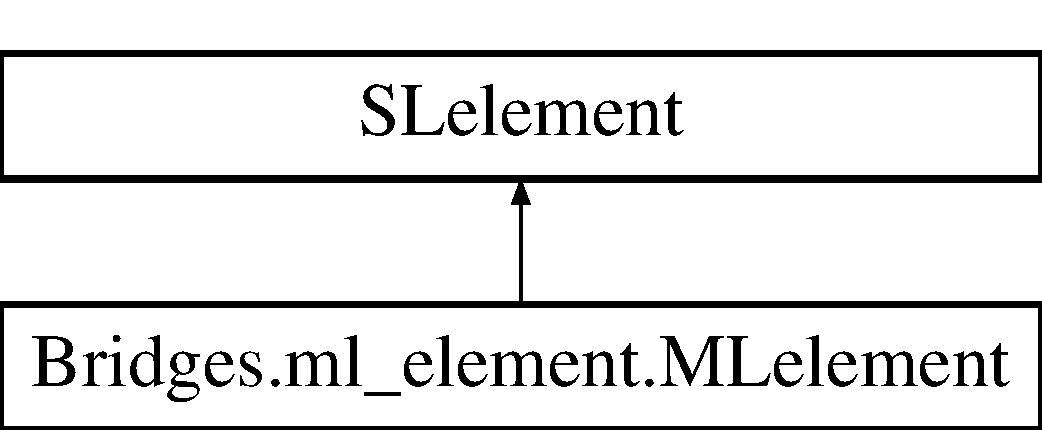
\includegraphics[height=2.000000cm]{class_bridges_1_1ml__element_1_1_m_lelement}
\end{center}
\end{figure}
\subsection*{Public Member Functions}
\begin{DoxyCompactItemize}
\item 
def \hyperlink{class_bridges_1_1ml__element_1_1_m_lelement_adf0e6222eabf94839df4106961c03a04}{\+\_\+\+\_\+init\+\_\+\+\_\+}
\begin{DoxyCompactList}\small\item\em This constructor creates an S\+Lelement object and sets the next pointer to null. \end{DoxyCompactList}\item 
def \hyperlink{class_bridges_1_1ml__element_1_1_m_lelement_ae1d401e972853ffab974aaa1dd44ab0e}{set\+\_\+sub\+\_\+list} (self, sl)
\begin{DoxyCompactList}\small\item\em Sets the start of a new sublist. \end{DoxyCompactList}\item 
def \hyperlink{class_bridges_1_1ml__element_1_1_m_lelement_ab60b9e960312e5210793bff87a6b81c8}{get\+\_\+sub\+\_\+list} (self)
\begin{DoxyCompactList}\small\item\em Gets the sublist at this node, if it exists. \end{DoxyCompactList}\item 
def \hyperlink{class_bridges_1_1ml__element_1_1_m_lelement_a66dc302580aedb52f17d138c54deceb2}{get\+\_\+data\+\_\+structure\+\_\+type} (self)
\begin{DoxyCompactList}\small\item\em This method gets the data structure type. \end{DoxyCompactList}\item 
def \hyperlink{class_bridges_1_1ml__element_1_1_m_lelement_ab4035d339d6133c3b2aab19028aafdf2}{get\+\_\+next} (self)
\begin{DoxyCompactList}\small\item\em Retrieves the element following this element. \end{DoxyCompactList}\item 
def \hyperlink{class_bridges_1_1ml__element_1_1_m_lelement_a5f093a6896365033a3a658a81b0024fe}{set\+\_\+tag} (self, t)
\begin{DoxyCompactList}\small\item\em Sets the tag of the element. \end{DoxyCompactList}\item 
def \hyperlink{class_bridges_1_1ml__element_1_1_m_lelement_a4657bdb7c765e5c0dac5e14fb6a61153}{get\+\_\+tag} (self)
\begin{DoxyCompactList}\small\item\em Gets the tag of the element. \end{DoxyCompactList}\item 
def \hyperlink{class_bridges_1_1ml__element_1_1_m_lelement_a3a511e7ec143ddc3a0ee5394dac76a0d}{get\+\_\+data\+\_\+structure\+\_\+representation} (self)
\item 
def \hyperlink{class_bridges_1_1ml__element_1_1_m_lelement_a6919e148ee1e2cf867f30240bf890ee7}{get\+\_\+list\+\_\+elements} (self, nodes)
\begin{DoxyCompactList}\small\item\em Get the elements of the list. \end{DoxyCompactList}\item 
def \hyperlink{class_bridges_1_1ml__element_1_1_m_lelement_a0bceedd612ad350144d1bc2cd0634291}{get\+\_\+list\+\_\+elements\+\_\+\+R} (self, list, nodes)
\end{DoxyCompactItemize}
\subsection*{Static Public Attributes}
\begin{DoxyCompactItemize}
\item 
\hyperlink{class_bridges_1_1ml__element_1_1_m_lelement_a08b50da0d31100920122df7df01c8abc}{sub\+\_\+list} = None
\item 
\hyperlink{class_bridges_1_1ml__element_1_1_m_lelement_aa9891ba8d6172b9ed65981f26036c213}{tag} = False
\end{DoxyCompactItemize}


\subsection{Detailed Description}
This class can be used to instantiate Multi-\/list Elements. 

This class extends S\+Lelement (singly linked list element) to build multi-\/lists; Multilist elements contain a tag that indicates if the element is a sublist or not; If the element points to a sublist, then the sublist field is the beginning of this sublist. If not, the data field contains the user specified data item and list continues (get\+Next()/set\+Next()). As in singly linked elements, the next pointer points to the following list element of the list or sublist.

Multi-\/list elements contain a visualizer (Element\+Visualizer) object for setting visual attributes (color, shape, opacity, size), necessary for displaying them in a web browser.

Elements also have a Link\+Visualizer object, that is used when they are linked to another element, appropriate for setting link attributes, for instance, between the current element and its next element. In this case, the link in question is that which connects the element to the following elements; a similar logic follows for sublists.

\begin{DoxyAuthor}{Author}
, Kalpathi Subramanian
\end{DoxyAuthor}
\begin{DoxyVerb}\sa Example Tutorial at <br> ??\end{DoxyVerb}
 

\subsection{Constructor \& Destructor Documentation}
\hypertarget{class_bridges_1_1ml__element_1_1_m_lelement_adf0e6222eabf94839df4106961c03a04}{}\index{Bridges\+::ml\+\_\+element\+::\+M\+Lelement@{Bridges\+::ml\+\_\+element\+::\+M\+Lelement}!\+\_\+\+\_\+init\+\_\+\+\_\+@{\+\_\+\+\_\+init\+\_\+\+\_\+}}
\index{\+\_\+\+\_\+init\+\_\+\+\_\+@{\+\_\+\+\_\+init\+\_\+\+\_\+}!Bridges\+::ml\+\_\+element\+::\+M\+Lelement@{Bridges\+::ml\+\_\+element\+::\+M\+Lelement}}
\subsubsection[{\+\_\+\+\_\+init\+\_\+\+\_\+}]{\setlength{\rightskip}{0pt plus 5cm}def Bridges.\+ml\+\_\+element.\+M\+Lelement.\+\_\+\+\_\+init\+\_\+\+\_\+ (
\begin{DoxyParamCaption}
\item[{}]{self, }
\item[{}]{label = {\ttfamily None}, }
\item[{}]{e = {\ttfamily None}, }
\item[{}]{next = {\ttfamily None}, }
\item[{}]{sublist = {\ttfamily None}}
\end{DoxyParamCaption}
)}\label{class_bridges_1_1ml__element_1_1_m_lelement_adf0e6222eabf94839df4106961c03a04}


This constructor creates an S\+Lelement object and sets the next pointer to null. 


\begin{DoxyParams}{Parameters}
{\em label} & the label of S\+Lelement that shows up on the bridges visualization \\
\hline
{\em e} & the generic object that this S\+Lelement will hold \\
\hline
{\em next} & the element that should be assigned to the next pointer \\
\hline
{\em sublist} & the \hyperlink{class_bridges_1_1ml__element_1_1_m_lelement}{M\+Lelement} that is the beginning of a sublist \\
\hline
\end{DoxyParams}


\subsection{Member Function Documentation}
\hypertarget{class_bridges_1_1ml__element_1_1_m_lelement_a3a511e7ec143ddc3a0ee5394dac76a0d}{}\index{Bridges\+::ml\+\_\+element\+::\+M\+Lelement@{Bridges\+::ml\+\_\+element\+::\+M\+Lelement}!get\+\_\+data\+\_\+structure\+\_\+representation@{get\+\_\+data\+\_\+structure\+\_\+representation}}
\index{get\+\_\+data\+\_\+structure\+\_\+representation@{get\+\_\+data\+\_\+structure\+\_\+representation}!Bridges\+::ml\+\_\+element\+::\+M\+Lelement@{Bridges\+::ml\+\_\+element\+::\+M\+Lelement}}
\subsubsection[{get\+\_\+data\+\_\+structure\+\_\+representation(self)}]{\setlength{\rightskip}{0pt plus 5cm}def Bridges.\+ml\+\_\+element.\+M\+Lelement.\+get\+\_\+data\+\_\+structure\+\_\+representation (
\begin{DoxyParamCaption}
\item[{}]{self}
\end{DoxyParamCaption}
)}\label{class_bridges_1_1ml__element_1_1_m_lelement_a3a511e7ec143ddc3a0ee5394dac76a0d}
\hypertarget{class_bridges_1_1ml__element_1_1_m_lelement_a66dc302580aedb52f17d138c54deceb2}{}\index{Bridges\+::ml\+\_\+element\+::\+M\+Lelement@{Bridges\+::ml\+\_\+element\+::\+M\+Lelement}!get\+\_\+data\+\_\+structure\+\_\+type@{get\+\_\+data\+\_\+structure\+\_\+type}}
\index{get\+\_\+data\+\_\+structure\+\_\+type@{get\+\_\+data\+\_\+structure\+\_\+type}!Bridges\+::ml\+\_\+element\+::\+M\+Lelement@{Bridges\+::ml\+\_\+element\+::\+M\+Lelement}}
\subsubsection[{get\+\_\+data\+\_\+structure\+\_\+type(self)}]{\setlength{\rightskip}{0pt plus 5cm}def Bridges.\+ml\+\_\+element.\+M\+Lelement.\+get\+\_\+data\+\_\+structure\+\_\+type (
\begin{DoxyParamCaption}
\item[{}]{self}
\end{DoxyParamCaption}
)}\label{class_bridges_1_1ml__element_1_1_m_lelement_a66dc302580aedb52f17d138c54deceb2}


This method gets the data structure type. 

\begin{DoxyReturn}{Returns}
The date structure type as a string 
\end{DoxyReturn}
\hypertarget{class_bridges_1_1ml__element_1_1_m_lelement_a6919e148ee1e2cf867f30240bf890ee7}{}\index{Bridges\+::ml\+\_\+element\+::\+M\+Lelement@{Bridges\+::ml\+\_\+element\+::\+M\+Lelement}!get\+\_\+list\+\_\+elements@{get\+\_\+list\+\_\+elements}}
\index{get\+\_\+list\+\_\+elements@{get\+\_\+list\+\_\+elements}!Bridges\+::ml\+\_\+element\+::\+M\+Lelement@{Bridges\+::ml\+\_\+element\+::\+M\+Lelement}}
\subsubsection[{get\+\_\+list\+\_\+elements(self, nodes)}]{\setlength{\rightskip}{0pt plus 5cm}def Bridges.\+ml\+\_\+element.\+M\+Lelement.\+get\+\_\+list\+\_\+elements (
\begin{DoxyParamCaption}
\item[{}]{self, }
\item[{}]{nodes}
\end{DoxyParamCaption}
)}\label{class_bridges_1_1ml__element_1_1_m_lelement_a6919e148ee1e2cf867f30240bf890ee7}


Get the elements of the list. 


\begin{DoxyParams}{Parameters}
{\em nodes} & a vector of the ndoes in the list \\
\hline
\end{DoxyParams}
\hypertarget{class_bridges_1_1ml__element_1_1_m_lelement_a0bceedd612ad350144d1bc2cd0634291}{}\index{Bridges\+::ml\+\_\+element\+::\+M\+Lelement@{Bridges\+::ml\+\_\+element\+::\+M\+Lelement}!get\+\_\+list\+\_\+elements\+\_\+\+R@{get\+\_\+list\+\_\+elements\+\_\+\+R}}
\index{get\+\_\+list\+\_\+elements\+\_\+\+R@{get\+\_\+list\+\_\+elements\+\_\+\+R}!Bridges\+::ml\+\_\+element\+::\+M\+Lelement@{Bridges\+::ml\+\_\+element\+::\+M\+Lelement}}
\subsubsection[{get\+\_\+list\+\_\+elements\+\_\+\+R(self, list, nodes)}]{\setlength{\rightskip}{0pt plus 5cm}def Bridges.\+ml\+\_\+element.\+M\+Lelement.\+get\+\_\+list\+\_\+elements\+\_\+\+R (
\begin{DoxyParamCaption}
\item[{}]{self, }
\item[{}]{list, }
\item[{}]{nodes}
\end{DoxyParamCaption}
)}\label{class_bridges_1_1ml__element_1_1_m_lelement_a0bceedd612ad350144d1bc2cd0634291}
\hypertarget{class_bridges_1_1ml__element_1_1_m_lelement_ab4035d339d6133c3b2aab19028aafdf2}{}\index{Bridges\+::ml\+\_\+element\+::\+M\+Lelement@{Bridges\+::ml\+\_\+element\+::\+M\+Lelement}!get\+\_\+next@{get\+\_\+next}}
\index{get\+\_\+next@{get\+\_\+next}!Bridges\+::ml\+\_\+element\+::\+M\+Lelement@{Bridges\+::ml\+\_\+element\+::\+M\+Lelement}}
\subsubsection[{get\+\_\+next(self)}]{\setlength{\rightskip}{0pt plus 5cm}def Bridges.\+ml\+\_\+element.\+M\+Lelement.\+get\+\_\+next (
\begin{DoxyParamCaption}
\item[{}]{self}
\end{DoxyParamCaption}
)}\label{class_bridges_1_1ml__element_1_1_m_lelement_ab4035d339d6133c3b2aab19028aafdf2}


Retrieves the element following this element. 

\begin{DoxyReturn}{Returns}
M\+Lelement$<$\+E$>$ assigned to next 
\end{DoxyReturn}
\hypertarget{class_bridges_1_1ml__element_1_1_m_lelement_ab60b9e960312e5210793bff87a6b81c8}{}\index{Bridges\+::ml\+\_\+element\+::\+M\+Lelement@{Bridges\+::ml\+\_\+element\+::\+M\+Lelement}!get\+\_\+sub\+\_\+list@{get\+\_\+sub\+\_\+list}}
\index{get\+\_\+sub\+\_\+list@{get\+\_\+sub\+\_\+list}!Bridges\+::ml\+\_\+element\+::\+M\+Lelement@{Bridges\+::ml\+\_\+element\+::\+M\+Lelement}}
\subsubsection[{get\+\_\+sub\+\_\+list(self)}]{\setlength{\rightskip}{0pt plus 5cm}def Bridges.\+ml\+\_\+element.\+M\+Lelement.\+get\+\_\+sub\+\_\+list (
\begin{DoxyParamCaption}
\item[{}]{self}
\end{DoxyParamCaption}
)}\label{class_bridges_1_1ml__element_1_1_m_lelement_ab60b9e960312e5210793bff87a6b81c8}


Gets the sublist at this node, if it exists. 

\begin{DoxyReturn}{Returns}
the sublist head element, if it exists 
\end{DoxyReturn}
\hypertarget{class_bridges_1_1ml__element_1_1_m_lelement_a4657bdb7c765e5c0dac5e14fb6a61153}{}\index{Bridges\+::ml\+\_\+element\+::\+M\+Lelement@{Bridges\+::ml\+\_\+element\+::\+M\+Lelement}!get\+\_\+tag@{get\+\_\+tag}}
\index{get\+\_\+tag@{get\+\_\+tag}!Bridges\+::ml\+\_\+element\+::\+M\+Lelement@{Bridges\+::ml\+\_\+element\+::\+M\+Lelement}}
\subsubsection[{get\+\_\+tag(self)}]{\setlength{\rightskip}{0pt plus 5cm}def Bridges.\+ml\+\_\+element.\+M\+Lelement.\+get\+\_\+tag (
\begin{DoxyParamCaption}
\item[{}]{self}
\end{DoxyParamCaption}
)}\label{class_bridges_1_1ml__element_1_1_m_lelement_a4657bdb7c765e5c0dac5e14fb6a61153}


Gets the tag of the element. 

\begin{DoxyReturn}{Returns}
tag of the element 
\end{DoxyReturn}
\hypertarget{class_bridges_1_1ml__element_1_1_m_lelement_ae1d401e972853ffab974aaa1dd44ab0e}{}\index{Bridges\+::ml\+\_\+element\+::\+M\+Lelement@{Bridges\+::ml\+\_\+element\+::\+M\+Lelement}!set\+\_\+sub\+\_\+list@{set\+\_\+sub\+\_\+list}}
\index{set\+\_\+sub\+\_\+list@{set\+\_\+sub\+\_\+list}!Bridges\+::ml\+\_\+element\+::\+M\+Lelement@{Bridges\+::ml\+\_\+element\+::\+M\+Lelement}}
\subsubsection[{set\+\_\+sub\+\_\+list(self, sl)}]{\setlength{\rightskip}{0pt plus 5cm}def Bridges.\+ml\+\_\+element.\+M\+Lelement.\+set\+\_\+sub\+\_\+list (
\begin{DoxyParamCaption}
\item[{}]{self, }
\item[{}]{sl}
\end{DoxyParamCaption}
)}\label{class_bridges_1_1ml__element_1_1_m_lelement_ae1d401e972853ffab974aaa1dd44ab0e}


Sets the start of a new sublist. 

to the S\+Lelement \char`\"{}next\char`\"{}


\begin{DoxyParams}{Parameters}
{\em sl} & the \hyperlink{class_bridges_1_1ml__element_1_1_m_lelement}{M\+Lelement} that is the beginning of a sublist \\
\hline
\end{DoxyParams}
\hypertarget{class_bridges_1_1ml__element_1_1_m_lelement_a5f093a6896365033a3a658a81b0024fe}{}\index{Bridges\+::ml\+\_\+element\+::\+M\+Lelement@{Bridges\+::ml\+\_\+element\+::\+M\+Lelement}!set\+\_\+tag@{set\+\_\+tag}}
\index{set\+\_\+tag@{set\+\_\+tag}!Bridges\+::ml\+\_\+element\+::\+M\+Lelement@{Bridges\+::ml\+\_\+element\+::\+M\+Lelement}}
\subsubsection[{set\+\_\+tag(self, t)}]{\setlength{\rightskip}{0pt plus 5cm}def Bridges.\+ml\+\_\+element.\+M\+Lelement.\+set\+\_\+tag (
\begin{DoxyParamCaption}
\item[{}]{self, }
\item[{}]{t}
\end{DoxyParamCaption}
)}\label{class_bridges_1_1ml__element_1_1_m_lelement_a5f093a6896365033a3a658a81b0024fe}


Sets the tag of the element. 


\begin{DoxyParams}{Parameters}
{\em boolean} & t \\
\hline
\end{DoxyParams}


\subsection{Member Data Documentation}
\hypertarget{class_bridges_1_1ml__element_1_1_m_lelement_a08b50da0d31100920122df7df01c8abc}{}\index{Bridges\+::ml\+\_\+element\+::\+M\+Lelement@{Bridges\+::ml\+\_\+element\+::\+M\+Lelement}!sub\+\_\+list@{sub\+\_\+list}}
\index{sub\+\_\+list@{sub\+\_\+list}!Bridges\+::ml\+\_\+element\+::\+M\+Lelement@{Bridges\+::ml\+\_\+element\+::\+M\+Lelement}}
\subsubsection[{sub\+\_\+list}]{\setlength{\rightskip}{0pt plus 5cm}Bridges.\+ml\+\_\+element.\+M\+Lelement.\+sub\+\_\+list = None\hspace{0.3cm}{\ttfamily [static]}}\label{class_bridges_1_1ml__element_1_1_m_lelement_a08b50da0d31100920122df7df01c8abc}
\hypertarget{class_bridges_1_1ml__element_1_1_m_lelement_aa9891ba8d6172b9ed65981f26036c213}{}\index{Bridges\+::ml\+\_\+element\+::\+M\+Lelement@{Bridges\+::ml\+\_\+element\+::\+M\+Lelement}!tag@{tag}}
\index{tag@{tag}!Bridges\+::ml\+\_\+element\+::\+M\+Lelement@{Bridges\+::ml\+\_\+element\+::\+M\+Lelement}}
\subsubsection[{tag}]{\setlength{\rightskip}{0pt plus 5cm}Bridges.\+ml\+\_\+element.\+M\+Lelement.\+tag = False\hspace{0.3cm}{\ttfamily [static]}}\label{class_bridges_1_1ml__element_1_1_m_lelement_aa9891ba8d6172b9ed65981f26036c213}


The documentation for this class was generated from the following file\+:\begin{DoxyCompactItemize}
\item 
/\+Users/kalpathi/gr/bridges/client/python/\+Bridges/\hyperlink{ml__element_8py}{ml\+\_\+element.\+py}\end{DoxyCompactItemize}

\hypertarget{class_bridges_1_1polygon_1_1_polygon}{}\section{Bridges.\+polygon.\+Polygon Class Reference}
\label{class_bridges_1_1polygon_1_1_polygon}\index{Bridges.\+polygon.\+Polygon@{Bridges.\+polygon.\+Polygon}}
Inheritance diagram for Bridges.\+polygon.\+Polygon\+:\begin{figure}[H]
\begin{center}
\leavevmode
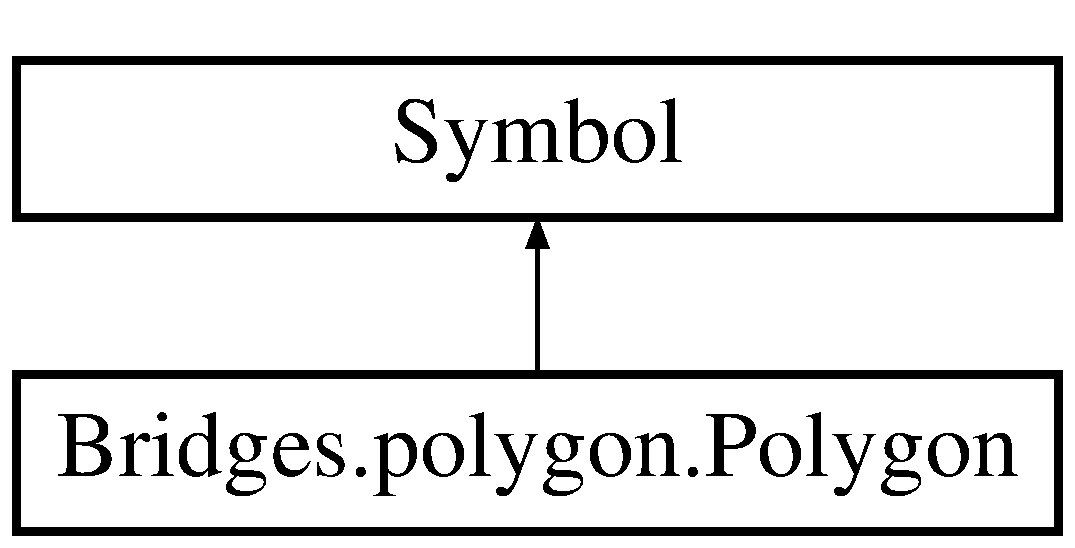
\includegraphics[height=2.000000cm]{class_bridges_1_1polygon_1_1_polygon}
\end{center}
\end{figure}
\subsection*{Public Member Functions}
\begin{DoxyCompactItemize}
\item 
def \mbox{\hyperlink{class_bridges_1_1polygon_1_1_polygon_a2fae05dc802684b344f111b274ac0c1a}{\+\_\+\+\_\+init\+\_\+\+\_\+}} (self, pts=None)
\item 
def \mbox{\hyperlink{class_bridges_1_1polygon_1_1_polygon_ac9356366dbc901727960f1453ebd5b9c}{get\+\_\+name}} (self)
\item 
def \mbox{\hyperlink{class_bridges_1_1polygon_1_1_polygon_a3c5d0d054fff18224cbd119c140f7992}{add\+\_\+point}} (self, x, y)
\item 
def \mbox{\hyperlink{class_bridges_1_1polygon_1_1_polygon_a2a4f182fb6f20ed0f4d2bef26ff4b856}{get\+\_\+points}} (self)
\item 
def \mbox{\hyperlink{class_bridges_1_1polygon_1_1_polygon_ac38b2fe8562b3419a8f2455cb0135f9b}{set\+\_\+polygon}} (self, pts)
\item 
def \mbox{\hyperlink{class_bridges_1_1polygon_1_1_polygon_a460fd0e58537beedf015ac7c092a6b8d}{get\+\_\+dimensions}} (self)
\item 
def \mbox{\hyperlink{class_bridges_1_1polygon_1_1_polygon_ac3ebc24755030ecad4508d8c89e7df9f}{get\+\_\+json\+\_\+representation}} (self)
\end{DoxyCompactItemize}
\subsection*{Public Attributes}
\begin{DoxyCompactItemize}
\item 
\mbox{\hyperlink{class_bridges_1_1polygon_1_1_polygon_a5303a39545d984b97ead1465ecbf9d1e}{points}}
\item 
\mbox{\hyperlink{class_bridges_1_1polygon_1_1_polygon_a764c8ae70e85104000e869dbcf23ac2c}{shape}}
\end{DoxyCompactItemize}


\subsection{Constructor \& Destructor Documentation}
\mbox{\Hypertarget{class_bridges_1_1polygon_1_1_polygon_a2fae05dc802684b344f111b274ac0c1a}\label{class_bridges_1_1polygon_1_1_polygon_a2fae05dc802684b344f111b274ac0c1a}} 
\index{Bridges\+::polygon\+::\+Polygon@{Bridges\+::polygon\+::\+Polygon}!\+\_\+\+\_\+init\+\_\+\+\_\+@{\+\_\+\+\_\+init\+\_\+\+\_\+}}
\index{\+\_\+\+\_\+init\+\_\+\+\_\+@{\+\_\+\+\_\+init\+\_\+\+\_\+}!Bridges\+::polygon\+::\+Polygon@{Bridges\+::polygon\+::\+Polygon}}
\subsubsection{\texorpdfstring{\+\_\+\+\_\+init\+\_\+\+\_\+()}{\_\_init\_\_()}}
{\footnotesize\ttfamily def Bridges.\+polygon.\+Polygon.\+\_\+\+\_\+init\+\_\+\+\_\+ (\begin{DoxyParamCaption}\item[{}]{self,  }\item[{}]{pts = {\ttfamily None} }\end{DoxyParamCaption})}



\subsection{Member Function Documentation}
\mbox{\Hypertarget{class_bridges_1_1polygon_1_1_polygon_a3c5d0d054fff18224cbd119c140f7992}\label{class_bridges_1_1polygon_1_1_polygon_a3c5d0d054fff18224cbd119c140f7992}} 
\index{Bridges\+::polygon\+::\+Polygon@{Bridges\+::polygon\+::\+Polygon}!add\+\_\+point@{add\+\_\+point}}
\index{add\+\_\+point@{add\+\_\+point}!Bridges\+::polygon\+::\+Polygon@{Bridges\+::polygon\+::\+Polygon}}
\subsubsection{\texorpdfstring{add\+\_\+point()}{add\_point()}}
{\footnotesize\ttfamily def Bridges.\+polygon.\+Polygon.\+add\+\_\+point (\begin{DoxyParamCaption}\item[{}]{self,  }\item[{}]{x,  }\item[{}]{y }\end{DoxyParamCaption})}

\mbox{\Hypertarget{class_bridges_1_1polygon_1_1_polygon_a460fd0e58537beedf015ac7c092a6b8d}\label{class_bridges_1_1polygon_1_1_polygon_a460fd0e58537beedf015ac7c092a6b8d}} 
\index{Bridges\+::polygon\+::\+Polygon@{Bridges\+::polygon\+::\+Polygon}!get\+\_\+dimensions@{get\+\_\+dimensions}}
\index{get\+\_\+dimensions@{get\+\_\+dimensions}!Bridges\+::polygon\+::\+Polygon@{Bridges\+::polygon\+::\+Polygon}}
\subsubsection{\texorpdfstring{get\+\_\+dimensions()}{get\_dimensions()}}
{\footnotesize\ttfamily def Bridges.\+polygon.\+Polygon.\+get\+\_\+dimensions (\begin{DoxyParamCaption}\item[{}]{self }\end{DoxyParamCaption})}

\mbox{\Hypertarget{class_bridges_1_1polygon_1_1_polygon_ac3ebc24755030ecad4508d8c89e7df9f}\label{class_bridges_1_1polygon_1_1_polygon_ac3ebc24755030ecad4508d8c89e7df9f}} 
\index{Bridges\+::polygon\+::\+Polygon@{Bridges\+::polygon\+::\+Polygon}!get\+\_\+json\+\_\+representation@{get\+\_\+json\+\_\+representation}}
\index{get\+\_\+json\+\_\+representation@{get\+\_\+json\+\_\+representation}!Bridges\+::polygon\+::\+Polygon@{Bridges\+::polygon\+::\+Polygon}}
\subsubsection{\texorpdfstring{get\+\_\+json\+\_\+representation()}{get\_json\_representation()}}
{\footnotesize\ttfamily def Bridges.\+polygon.\+Polygon.\+get\+\_\+json\+\_\+representation (\begin{DoxyParamCaption}\item[{}]{self }\end{DoxyParamCaption})}

\mbox{\Hypertarget{class_bridges_1_1polygon_1_1_polygon_ac9356366dbc901727960f1453ebd5b9c}\label{class_bridges_1_1polygon_1_1_polygon_ac9356366dbc901727960f1453ebd5b9c}} 
\index{Bridges\+::polygon\+::\+Polygon@{Bridges\+::polygon\+::\+Polygon}!get\+\_\+name@{get\+\_\+name}}
\index{get\+\_\+name@{get\+\_\+name}!Bridges\+::polygon\+::\+Polygon@{Bridges\+::polygon\+::\+Polygon}}
\subsubsection{\texorpdfstring{get\+\_\+name()}{get\_name()}}
{\footnotesize\ttfamily def Bridges.\+polygon.\+Polygon.\+get\+\_\+name (\begin{DoxyParamCaption}\item[{}]{self }\end{DoxyParamCaption})}

\mbox{\Hypertarget{class_bridges_1_1polygon_1_1_polygon_a2a4f182fb6f20ed0f4d2bef26ff4b856}\label{class_bridges_1_1polygon_1_1_polygon_a2a4f182fb6f20ed0f4d2bef26ff4b856}} 
\index{Bridges\+::polygon\+::\+Polygon@{Bridges\+::polygon\+::\+Polygon}!get\+\_\+points@{get\+\_\+points}}
\index{get\+\_\+points@{get\+\_\+points}!Bridges\+::polygon\+::\+Polygon@{Bridges\+::polygon\+::\+Polygon}}
\subsubsection{\texorpdfstring{get\+\_\+points()}{get\_points()}}
{\footnotesize\ttfamily def Bridges.\+polygon.\+Polygon.\+get\+\_\+points (\begin{DoxyParamCaption}\item[{}]{self }\end{DoxyParamCaption})}

\mbox{\Hypertarget{class_bridges_1_1polygon_1_1_polygon_ac38b2fe8562b3419a8f2455cb0135f9b}\label{class_bridges_1_1polygon_1_1_polygon_ac38b2fe8562b3419a8f2455cb0135f9b}} 
\index{Bridges\+::polygon\+::\+Polygon@{Bridges\+::polygon\+::\+Polygon}!set\+\_\+polygon@{set\+\_\+polygon}}
\index{set\+\_\+polygon@{set\+\_\+polygon}!Bridges\+::polygon\+::\+Polygon@{Bridges\+::polygon\+::\+Polygon}}
\subsubsection{\texorpdfstring{set\+\_\+polygon()}{set\_polygon()}}
{\footnotesize\ttfamily def Bridges.\+polygon.\+Polygon.\+set\+\_\+polygon (\begin{DoxyParamCaption}\item[{}]{self,  }\item[{}]{pts }\end{DoxyParamCaption})}



\subsection{Member Data Documentation}
\mbox{\Hypertarget{class_bridges_1_1polygon_1_1_polygon_a5303a39545d984b97ead1465ecbf9d1e}\label{class_bridges_1_1polygon_1_1_polygon_a5303a39545d984b97ead1465ecbf9d1e}} 
\index{Bridges\+::polygon\+::\+Polygon@{Bridges\+::polygon\+::\+Polygon}!points@{points}}
\index{points@{points}!Bridges\+::polygon\+::\+Polygon@{Bridges\+::polygon\+::\+Polygon}}
\subsubsection{\texorpdfstring{points}{points}}
{\footnotesize\ttfamily Bridges.\+polygon.\+Polygon.\+points}

\mbox{\Hypertarget{class_bridges_1_1polygon_1_1_polygon_a764c8ae70e85104000e869dbcf23ac2c}\label{class_bridges_1_1polygon_1_1_polygon_a764c8ae70e85104000e869dbcf23ac2c}} 
\index{Bridges\+::polygon\+::\+Polygon@{Bridges\+::polygon\+::\+Polygon}!shape@{shape}}
\index{shape@{shape}!Bridges\+::polygon\+::\+Polygon@{Bridges\+::polygon\+::\+Polygon}}
\subsubsection{\texorpdfstring{shape}{shape}}
{\footnotesize\ttfamily Bridges.\+polygon.\+Polygon.\+shape}



The documentation for this class was generated from the following file\+:\begin{DoxyCompactItemize}
\item 
/\+Users/kalpathi/gr/bridges/client/python/bridges18/\+Bridges/\mbox{\hyperlink{polygon_8py}{polygon.\+py}}\end{DoxyCompactItemize}

\hypertarget{class_bridges_1_1rectangle_1_1_rectangle}{}\section{Bridges.\+rectangle.\+Rectangle Class Reference}
\label{class_bridges_1_1rectangle_1_1_rectangle}\index{Bridges.\+rectangle.\+Rectangle@{Bridges.\+rectangle.\+Rectangle}}
Inheritance diagram for Bridges.\+rectangle.\+Rectangle\+:\begin{figure}[H]
\begin{center}
\leavevmode
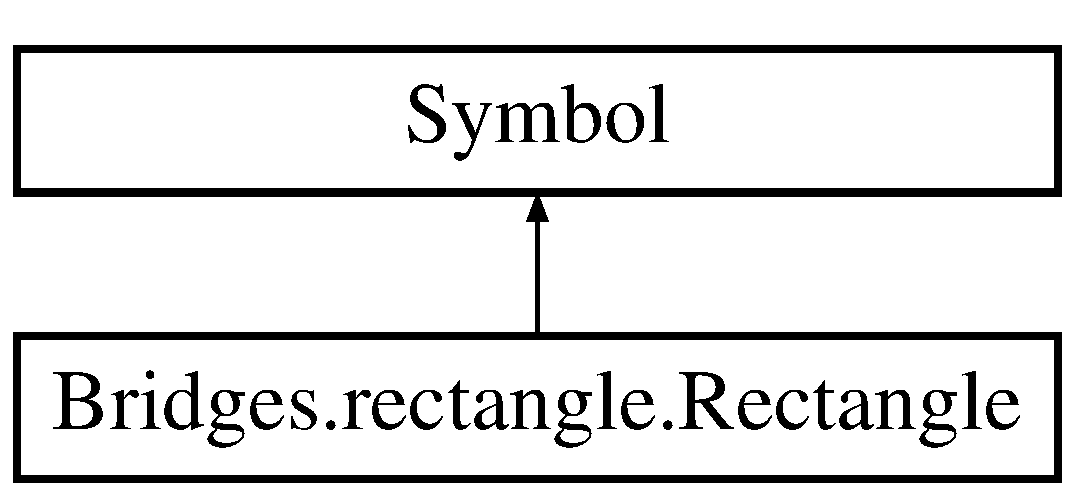
\includegraphics[height=2.000000cm]{class_bridges_1_1rectangle_1_1_rectangle}
\end{center}
\end{figure}
\subsection*{Public Member Functions}
\begin{DoxyCompactItemize}
\item 
def \mbox{\hyperlink{class_bridges_1_1rectangle_1_1_rectangle_aac3556ec035b237c15365ff5a23206f3}{\+\_\+\+\_\+init\+\_\+\+\_\+}} (self, w=None, h=None, locx=None, locy=None)
\item 
def \mbox{\hyperlink{class_bridges_1_1rectangle_1_1_rectangle_a6f2180be9e39b4e8ebb83dde0d2ae2e1}{get\+\_\+name}} (self)
\item 
def \mbox{\hyperlink{class_bridges_1_1rectangle_1_1_rectangle_a2f856ecb4decb067e258e4e9f7b2ad00}{set\+\_\+width}} (self, w)
\item 
def \mbox{\hyperlink{class_bridges_1_1rectangle_1_1_rectangle_a43141b79a309d329a166ddd6125f3fb7}{set\+\_\+height}} (self, h)
\item 
def \mbox{\hyperlink{class_bridges_1_1rectangle_1_1_rectangle_a63c94bd3ac867e615755664e70020cac}{get\+\_\+dimensions}} (self)
\item 
def \mbox{\hyperlink{class_bridges_1_1rectangle_1_1_rectangle_a140506622c30bf1e384b4c3d71892351}{set\+\_\+rectangle}} (self, locx, locy, w, h)
\item 
def \mbox{\hyperlink{class_bridges_1_1rectangle_1_1_rectangle_a5d45f960a05924df3184abf86085392b}{get\+\_\+json\+\_\+representation}} (self)
\end{DoxyCompactItemize}
\subsection*{Public Attributes}
\begin{DoxyCompactItemize}
\item 
\mbox{\hyperlink{class_bridges_1_1rectangle_1_1_rectangle_aaae9ea88bf002ce04c7a1b790d5e6426}{width}}
\item 
\mbox{\hyperlink{class_bridges_1_1rectangle_1_1_rectangle_a43de3ad0b917af8d8bb107e3113f6414}{height}}
\end{DoxyCompactItemize}


\subsection{Constructor \& Destructor Documentation}
\mbox{\Hypertarget{class_bridges_1_1rectangle_1_1_rectangle_aac3556ec035b237c15365ff5a23206f3}\label{class_bridges_1_1rectangle_1_1_rectangle_aac3556ec035b237c15365ff5a23206f3}} 
\index{Bridges\+::rectangle\+::\+Rectangle@{Bridges\+::rectangle\+::\+Rectangle}!\+\_\+\+\_\+init\+\_\+\+\_\+@{\+\_\+\+\_\+init\+\_\+\+\_\+}}
\index{\+\_\+\+\_\+init\+\_\+\+\_\+@{\+\_\+\+\_\+init\+\_\+\+\_\+}!Bridges\+::rectangle\+::\+Rectangle@{Bridges\+::rectangle\+::\+Rectangle}}
\subsubsection{\texorpdfstring{\+\_\+\+\_\+init\+\_\+\+\_\+()}{\_\_init\_\_()}}
{\footnotesize\ttfamily def Bridges.\+rectangle.\+Rectangle.\+\_\+\+\_\+init\+\_\+\+\_\+ (\begin{DoxyParamCaption}\item[{}]{self,  }\item[{}]{w = {\ttfamily None},  }\item[{}]{h = {\ttfamily None},  }\item[{}]{locx = {\ttfamily None},  }\item[{}]{locy = {\ttfamily None} }\end{DoxyParamCaption})}



\subsection{Member Function Documentation}
\mbox{\Hypertarget{class_bridges_1_1rectangle_1_1_rectangle_a63c94bd3ac867e615755664e70020cac}\label{class_bridges_1_1rectangle_1_1_rectangle_a63c94bd3ac867e615755664e70020cac}} 
\index{Bridges\+::rectangle\+::\+Rectangle@{Bridges\+::rectangle\+::\+Rectangle}!get\+\_\+dimensions@{get\+\_\+dimensions}}
\index{get\+\_\+dimensions@{get\+\_\+dimensions}!Bridges\+::rectangle\+::\+Rectangle@{Bridges\+::rectangle\+::\+Rectangle}}
\subsubsection{\texorpdfstring{get\+\_\+dimensions()}{get\_dimensions()}}
{\footnotesize\ttfamily def Bridges.\+rectangle.\+Rectangle.\+get\+\_\+dimensions (\begin{DoxyParamCaption}\item[{}]{self }\end{DoxyParamCaption})}

\mbox{\Hypertarget{class_bridges_1_1rectangle_1_1_rectangle_a5d45f960a05924df3184abf86085392b}\label{class_bridges_1_1rectangle_1_1_rectangle_a5d45f960a05924df3184abf86085392b}} 
\index{Bridges\+::rectangle\+::\+Rectangle@{Bridges\+::rectangle\+::\+Rectangle}!get\+\_\+json\+\_\+representation@{get\+\_\+json\+\_\+representation}}
\index{get\+\_\+json\+\_\+representation@{get\+\_\+json\+\_\+representation}!Bridges\+::rectangle\+::\+Rectangle@{Bridges\+::rectangle\+::\+Rectangle}}
\subsubsection{\texorpdfstring{get\+\_\+json\+\_\+representation()}{get\_json\_representation()}}
{\footnotesize\ttfamily def Bridges.\+rectangle.\+Rectangle.\+get\+\_\+json\+\_\+representation (\begin{DoxyParamCaption}\item[{}]{self }\end{DoxyParamCaption})}

\mbox{\Hypertarget{class_bridges_1_1rectangle_1_1_rectangle_a6f2180be9e39b4e8ebb83dde0d2ae2e1}\label{class_bridges_1_1rectangle_1_1_rectangle_a6f2180be9e39b4e8ebb83dde0d2ae2e1}} 
\index{Bridges\+::rectangle\+::\+Rectangle@{Bridges\+::rectangle\+::\+Rectangle}!get\+\_\+name@{get\+\_\+name}}
\index{get\+\_\+name@{get\+\_\+name}!Bridges\+::rectangle\+::\+Rectangle@{Bridges\+::rectangle\+::\+Rectangle}}
\subsubsection{\texorpdfstring{get\+\_\+name()}{get\_name()}}
{\footnotesize\ttfamily def Bridges.\+rectangle.\+Rectangle.\+get\+\_\+name (\begin{DoxyParamCaption}\item[{}]{self }\end{DoxyParamCaption})}

\mbox{\Hypertarget{class_bridges_1_1rectangle_1_1_rectangle_a43141b79a309d329a166ddd6125f3fb7}\label{class_bridges_1_1rectangle_1_1_rectangle_a43141b79a309d329a166ddd6125f3fb7}} 
\index{Bridges\+::rectangle\+::\+Rectangle@{Bridges\+::rectangle\+::\+Rectangle}!set\+\_\+height@{set\+\_\+height}}
\index{set\+\_\+height@{set\+\_\+height}!Bridges\+::rectangle\+::\+Rectangle@{Bridges\+::rectangle\+::\+Rectangle}}
\subsubsection{\texorpdfstring{set\+\_\+height()}{set\_height()}}
{\footnotesize\ttfamily def Bridges.\+rectangle.\+Rectangle.\+set\+\_\+height (\begin{DoxyParamCaption}\item[{}]{self,  }\item[{}]{h }\end{DoxyParamCaption})}

\mbox{\Hypertarget{class_bridges_1_1rectangle_1_1_rectangle_a140506622c30bf1e384b4c3d71892351}\label{class_bridges_1_1rectangle_1_1_rectangle_a140506622c30bf1e384b4c3d71892351}} 
\index{Bridges\+::rectangle\+::\+Rectangle@{Bridges\+::rectangle\+::\+Rectangle}!set\+\_\+rectangle@{set\+\_\+rectangle}}
\index{set\+\_\+rectangle@{set\+\_\+rectangle}!Bridges\+::rectangle\+::\+Rectangle@{Bridges\+::rectangle\+::\+Rectangle}}
\subsubsection{\texorpdfstring{set\+\_\+rectangle()}{set\_rectangle()}}
{\footnotesize\ttfamily def Bridges.\+rectangle.\+Rectangle.\+set\+\_\+rectangle (\begin{DoxyParamCaption}\item[{}]{self,  }\item[{}]{locx,  }\item[{}]{locy,  }\item[{}]{w,  }\item[{}]{h }\end{DoxyParamCaption})}

\mbox{\Hypertarget{class_bridges_1_1rectangle_1_1_rectangle_a2f856ecb4decb067e258e4e9f7b2ad00}\label{class_bridges_1_1rectangle_1_1_rectangle_a2f856ecb4decb067e258e4e9f7b2ad00}} 
\index{Bridges\+::rectangle\+::\+Rectangle@{Bridges\+::rectangle\+::\+Rectangle}!set\+\_\+width@{set\+\_\+width}}
\index{set\+\_\+width@{set\+\_\+width}!Bridges\+::rectangle\+::\+Rectangle@{Bridges\+::rectangle\+::\+Rectangle}}
\subsubsection{\texorpdfstring{set\+\_\+width()}{set\_width()}}
{\footnotesize\ttfamily def Bridges.\+rectangle.\+Rectangle.\+set\+\_\+width (\begin{DoxyParamCaption}\item[{}]{self,  }\item[{}]{w }\end{DoxyParamCaption})}



\subsection{Member Data Documentation}
\mbox{\Hypertarget{class_bridges_1_1rectangle_1_1_rectangle_a43de3ad0b917af8d8bb107e3113f6414}\label{class_bridges_1_1rectangle_1_1_rectangle_a43de3ad0b917af8d8bb107e3113f6414}} 
\index{Bridges\+::rectangle\+::\+Rectangle@{Bridges\+::rectangle\+::\+Rectangle}!height@{height}}
\index{height@{height}!Bridges\+::rectangle\+::\+Rectangle@{Bridges\+::rectangle\+::\+Rectangle}}
\subsubsection{\texorpdfstring{height}{height}}
{\footnotesize\ttfamily Bridges.\+rectangle.\+Rectangle.\+height}

\mbox{\Hypertarget{class_bridges_1_1rectangle_1_1_rectangle_aaae9ea88bf002ce04c7a1b790d5e6426}\label{class_bridges_1_1rectangle_1_1_rectangle_aaae9ea88bf002ce04c7a1b790d5e6426}} 
\index{Bridges\+::rectangle\+::\+Rectangle@{Bridges\+::rectangle\+::\+Rectangle}!width@{width}}
\index{width@{width}!Bridges\+::rectangle\+::\+Rectangle@{Bridges\+::rectangle\+::\+Rectangle}}
\subsubsection{\texorpdfstring{width}{width}}
{\footnotesize\ttfamily Bridges.\+rectangle.\+Rectangle.\+width}



The documentation for this class was generated from the following file\+:\begin{DoxyCompactItemize}
\item 
/\+Users/kalpathi/gr/bridges/client/python/bridges18/\+Bridges/\mbox{\hyperlink{rectangle_8py}{rectangle.\+py}}\end{DoxyCompactItemize}

\hypertarget{class_bridges_1_1sl__element_1_1_s_lelement}{}\section{Bridges.\+sl\+\_\+element.\+S\+Lelement Class Reference}
\label{class_bridges_1_1sl__element_1_1_s_lelement}\index{Bridges.\+sl\+\_\+element.\+S\+Lelement@{Bridges.\+sl\+\_\+element.\+S\+Lelement}}


This class can be used to instantiate Singly Linked Elements.  


Inheritance diagram for Bridges.\+sl\+\_\+element.\+S\+Lelement\+:\begin{figure}[H]
\begin{center}
\leavevmode
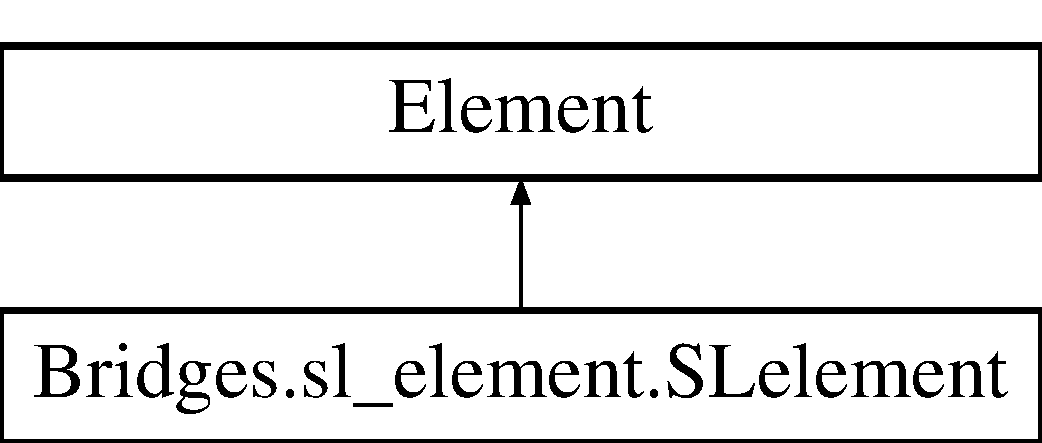
\includegraphics[height=2.000000cm]{class_bridges_1_1sl__element_1_1_s_lelement}
\end{center}
\end{figure}
\subsection*{Public Member Functions}
\begin{DoxyCompactItemize}
\item 
def \hyperlink{class_bridges_1_1sl__element_1_1_s_lelement_a7d6fa5bfb29d5b0e1cb1b7bf993391a5}{\+\_\+\+\_\+init\+\_\+\+\_\+}
\begin{DoxyCompactList}\small\item\em This constructor creates an \hyperlink{class_bridges_1_1sl__element_1_1_s_lelement}{S\+Lelement} object and sets the next pointer to null. \end{DoxyCompactList}\item 
def \hyperlink{class_bridges_1_1sl__element_1_1_s_lelement_a64621ee79ab3420c38f11f75c8af94e4}{get\+\_\+data\+\_\+structure\+\_\+type} (self)
\begin{DoxyCompactList}\small\item\em This method gets the data structure type. \end{DoxyCompactList}\item 
def \hyperlink{class_bridges_1_1sl__element_1_1_s_lelement_a9767c8fd4d69a721014d659f9d07dfe8}{get\+\_\+next} (self)
\begin{DoxyCompactList}\small\item\em Retrieves the element following this element. \end{DoxyCompactList}\item 
def \hyperlink{class_bridges_1_1sl__element_1_1_s_lelement_a2f489dc7aa2602c4bbb295a1cb4d4efb}{get\+\_\+value} (self)
\item 
def \hyperlink{class_bridges_1_1sl__element_1_1_s_lelement_a1db3bb6e3360c62fa293c2e5df7a93b3}{set\+\_\+next} (self, \hyperlink{class_bridges_1_1sl__element_1_1_s_lelement_a96a8af8acbfe6f35cfdd1fd8ab16281d}{next})
\begin{DoxyCompactList}\small\item\em Sets the element to point to the next \hyperlink{class_bridges_1_1sl__element_1_1_s_lelement}{S\+Lelement}. \end{DoxyCompactList}\item 
def \hyperlink{class_bridges_1_1sl__element_1_1_s_lelement_ae5cba7dbda33046b4cb47b6f08e0245c}{\+\_\+\+\_\+str\+\_\+\+\_\+} (self)
\item 
def \hyperlink{class_bridges_1_1sl__element_1_1_s_lelement_a840ee42b8296ef3380771aac60d352c3}{get\+\_\+data\+\_\+structure\+\_\+representation} (self)
\begin{DoxyCompactList}\small\item\em Get the J\+S\+O\+N representation of the the data structure. \end{DoxyCompactList}\item 
def \hyperlink{class_bridges_1_1sl__element_1_1_s_lelement_ac25a593141f89b0ca10ce2a083bac309}{get\+\_\+list\+\_\+elements} (self, nodes)
\begin{DoxyCompactList}\small\item\em Get the elements of the list. \end{DoxyCompactList}\end{DoxyCompactItemize}
\subsection*{Public Attributes}
\begin{DoxyCompactItemize}
\item 
\hyperlink{class_bridges_1_1sl__element_1_1_s_lelement_a96a8af8acbfe6f35cfdd1fd8ab16281d}{next}
\end{DoxyCompactItemize}


\subsection{Detailed Description}
This class can be used to instantiate Singly Linked Elements. 

This class extends Element and takes a generic parameter $<$\+E$>$ representing application specific data. This element forms the basic building block for singly linked lists. Singly linked elements have a field pointing to the next element along the list.

\begin{DoxyVerb}Elements contain a visualizer (ElementVisualizer) object for setting visual
attributes (color, shape, opacity, size), necessary for displaying them in a
web browser.

Elements also have a LinkVisualizer object, that is used when they are linked to
another element, appropriate for setting link attributes, for instance, between
the current element and its next element.
\end{DoxyVerb}


\begin{DoxyAuthor}{Author}
Mihai Mehedint, Kalpathi Subramanian
\end{DoxyAuthor}
\begin{DoxyDate}{Date}
6/22/16, 1/7/17, 5/17/17
\end{DoxyDate}

\begin{DoxyParams}{Parameters}
{\em $<$\+E$>$} & The generic parameter object that is part of this element, representing application specific data.\\
\hline
\end{DoxyParams}
\begin{DoxySeeAlso}{See also}
Example Tutorial at ~\newline
 \href{http://bridgesuncc.github.io/Hello_World_Tutorials/SLL.html}{\tt http\+://bridgesuncc.\+github.\+io/\+Hello\+\_\+\+World\+\_\+\+Tutorials/\+S\+L\+L.\+html} 
\end{DoxySeeAlso}


\subsection{Constructor \& Destructor Documentation}
\hypertarget{class_bridges_1_1sl__element_1_1_s_lelement_a7d6fa5bfb29d5b0e1cb1b7bf993391a5}{}\index{Bridges\+::sl\+\_\+element\+::\+S\+Lelement@{Bridges\+::sl\+\_\+element\+::\+S\+Lelement}!\+\_\+\+\_\+init\+\_\+\+\_\+@{\+\_\+\+\_\+init\+\_\+\+\_\+}}
\index{\+\_\+\+\_\+init\+\_\+\+\_\+@{\+\_\+\+\_\+init\+\_\+\+\_\+}!Bridges\+::sl\+\_\+element\+::\+S\+Lelement@{Bridges\+::sl\+\_\+element\+::\+S\+Lelement}}
\subsubsection[{\+\_\+\+\_\+init\+\_\+\+\_\+}]{\setlength{\rightskip}{0pt plus 5cm}def Bridges.\+sl\+\_\+element.\+S\+Lelement.\+\_\+\+\_\+init\+\_\+\+\_\+ (
\begin{DoxyParamCaption}
\item[{}]{self, }
\item[{}]{e = {\ttfamily None}, }
\item[{}]{label = {\ttfamily None}, }
\item[{}]{next = {\ttfamily None}}
\end{DoxyParamCaption}
)}\label{class_bridges_1_1sl__element_1_1_s_lelement_a7d6fa5bfb29d5b0e1cb1b7bf993391a5}


This constructor creates an \hyperlink{class_bridges_1_1sl__element_1_1_s_lelement}{S\+Lelement} object and sets the next pointer to null. 


\begin{DoxyParams}{Parameters}
{\em label} & the label of \hyperlink{class_bridges_1_1sl__element_1_1_s_lelement}{S\+Lelement} that shows up on the bridges visualization \\
\hline
{\em e} & the generic object that this \hyperlink{class_bridges_1_1sl__element_1_1_s_lelement}{S\+Lelement} will hold \\
\hline
{\em next} & the element that should be assigned to the next pointer \\
\hline
\end{DoxyParams}


\subsection{Member Function Documentation}
\hypertarget{class_bridges_1_1sl__element_1_1_s_lelement_ae5cba7dbda33046b4cb47b6f08e0245c}{}\index{Bridges\+::sl\+\_\+element\+::\+S\+Lelement@{Bridges\+::sl\+\_\+element\+::\+S\+Lelement}!\+\_\+\+\_\+str\+\_\+\+\_\+@{\+\_\+\+\_\+str\+\_\+\+\_\+}}
\index{\+\_\+\+\_\+str\+\_\+\+\_\+@{\+\_\+\+\_\+str\+\_\+\+\_\+}!Bridges\+::sl\+\_\+element\+::\+S\+Lelement@{Bridges\+::sl\+\_\+element\+::\+S\+Lelement}}
\subsubsection[{\+\_\+\+\_\+str\+\_\+\+\_\+(self)}]{\setlength{\rightskip}{0pt plus 5cm}def Bridges.\+sl\+\_\+element.\+S\+Lelement.\+\_\+\+\_\+str\+\_\+\+\_\+ (
\begin{DoxyParamCaption}
\item[{}]{self}
\end{DoxyParamCaption}
)}\label{class_bridges_1_1sl__element_1_1_s_lelement_ae5cba7dbda33046b4cb47b6f08e0245c}
\hypertarget{class_bridges_1_1sl__element_1_1_s_lelement_a840ee42b8296ef3380771aac60d352c3}{}\index{Bridges\+::sl\+\_\+element\+::\+S\+Lelement@{Bridges\+::sl\+\_\+element\+::\+S\+Lelement}!get\+\_\+data\+\_\+structure\+\_\+representation@{get\+\_\+data\+\_\+structure\+\_\+representation}}
\index{get\+\_\+data\+\_\+structure\+\_\+representation@{get\+\_\+data\+\_\+structure\+\_\+representation}!Bridges\+::sl\+\_\+element\+::\+S\+Lelement@{Bridges\+::sl\+\_\+element\+::\+S\+Lelement}}
\subsubsection[{get\+\_\+data\+\_\+structure\+\_\+representation(self)}]{\setlength{\rightskip}{0pt plus 5cm}def Bridges.\+sl\+\_\+element.\+S\+Lelement.\+get\+\_\+data\+\_\+structure\+\_\+representation (
\begin{DoxyParamCaption}
\item[{}]{self}
\end{DoxyParamCaption}
)}\label{class_bridges_1_1sl__element_1_1_s_lelement_a840ee42b8296ef3380771aac60d352c3}


Get the J\+S\+O\+N representation of the the data structure. 

\hypertarget{class_bridges_1_1sl__element_1_1_s_lelement_a64621ee79ab3420c38f11f75c8af94e4}{}\index{Bridges\+::sl\+\_\+element\+::\+S\+Lelement@{Bridges\+::sl\+\_\+element\+::\+S\+Lelement}!get\+\_\+data\+\_\+structure\+\_\+type@{get\+\_\+data\+\_\+structure\+\_\+type}}
\index{get\+\_\+data\+\_\+structure\+\_\+type@{get\+\_\+data\+\_\+structure\+\_\+type}!Bridges\+::sl\+\_\+element\+::\+S\+Lelement@{Bridges\+::sl\+\_\+element\+::\+S\+Lelement}}
\subsubsection[{get\+\_\+data\+\_\+structure\+\_\+type(self)}]{\setlength{\rightskip}{0pt plus 5cm}def Bridges.\+sl\+\_\+element.\+S\+Lelement.\+get\+\_\+data\+\_\+structure\+\_\+type (
\begin{DoxyParamCaption}
\item[{}]{self}
\end{DoxyParamCaption}
)}\label{class_bridges_1_1sl__element_1_1_s_lelement_a64621ee79ab3420c38f11f75c8af94e4}


This method gets the data structure type. 

\begin{DoxyReturn}{Returns}
The date structure type as a string 
\end{DoxyReturn}
\hypertarget{class_bridges_1_1sl__element_1_1_s_lelement_ac25a593141f89b0ca10ce2a083bac309}{}\index{Bridges\+::sl\+\_\+element\+::\+S\+Lelement@{Bridges\+::sl\+\_\+element\+::\+S\+Lelement}!get\+\_\+list\+\_\+elements@{get\+\_\+list\+\_\+elements}}
\index{get\+\_\+list\+\_\+elements@{get\+\_\+list\+\_\+elements}!Bridges\+::sl\+\_\+element\+::\+S\+Lelement@{Bridges\+::sl\+\_\+element\+::\+S\+Lelement}}
\subsubsection[{get\+\_\+list\+\_\+elements(self, nodes)}]{\setlength{\rightskip}{0pt plus 5cm}def Bridges.\+sl\+\_\+element.\+S\+Lelement.\+get\+\_\+list\+\_\+elements (
\begin{DoxyParamCaption}
\item[{}]{self, }
\item[{}]{nodes}
\end{DoxyParamCaption}
)}\label{class_bridges_1_1sl__element_1_1_s_lelement_ac25a593141f89b0ca10ce2a083bac309}


Get the elements of the list. 


\begin{DoxyParams}{Parameters}
{\em nodes} & a vector of the ndoes in the list \\
\hline
\end{DoxyParams}
\hypertarget{class_bridges_1_1sl__element_1_1_s_lelement_a9767c8fd4d69a721014d659f9d07dfe8}{}\index{Bridges\+::sl\+\_\+element\+::\+S\+Lelement@{Bridges\+::sl\+\_\+element\+::\+S\+Lelement}!get\+\_\+next@{get\+\_\+next}}
\index{get\+\_\+next@{get\+\_\+next}!Bridges\+::sl\+\_\+element\+::\+S\+Lelement@{Bridges\+::sl\+\_\+element\+::\+S\+Lelement}}
\subsubsection[{get\+\_\+next(self)}]{\setlength{\rightskip}{0pt plus 5cm}def Bridges.\+sl\+\_\+element.\+S\+Lelement.\+get\+\_\+next (
\begin{DoxyParamCaption}
\item[{}]{self}
\end{DoxyParamCaption}
)}\label{class_bridges_1_1sl__element_1_1_s_lelement_a9767c8fd4d69a721014d659f9d07dfe8}


Retrieves the element following this element. 

\begin{DoxyReturn}{Returns}
S\+Lelement$<$\+E$>$ assigned to next 
\end{DoxyReturn}
\hypertarget{class_bridges_1_1sl__element_1_1_s_lelement_a2f489dc7aa2602c4bbb295a1cb4d4efb}{}\index{Bridges\+::sl\+\_\+element\+::\+S\+Lelement@{Bridges\+::sl\+\_\+element\+::\+S\+Lelement}!get\+\_\+value@{get\+\_\+value}}
\index{get\+\_\+value@{get\+\_\+value}!Bridges\+::sl\+\_\+element\+::\+S\+Lelement@{Bridges\+::sl\+\_\+element\+::\+S\+Lelement}}
\subsubsection[{get\+\_\+value(self)}]{\setlength{\rightskip}{0pt plus 5cm}def Bridges.\+sl\+\_\+element.\+S\+Lelement.\+get\+\_\+value (
\begin{DoxyParamCaption}
\item[{}]{self}
\end{DoxyParamCaption}
)}\label{class_bridges_1_1sl__element_1_1_s_lelement_a2f489dc7aa2602c4bbb295a1cb4d4efb}
\hypertarget{class_bridges_1_1sl__element_1_1_s_lelement_a1db3bb6e3360c62fa293c2e5df7a93b3}{}\index{Bridges\+::sl\+\_\+element\+::\+S\+Lelement@{Bridges\+::sl\+\_\+element\+::\+S\+Lelement}!set\+\_\+next@{set\+\_\+next}}
\index{set\+\_\+next@{set\+\_\+next}!Bridges\+::sl\+\_\+element\+::\+S\+Lelement@{Bridges\+::sl\+\_\+element\+::\+S\+Lelement}}
\subsubsection[{set\+\_\+next(self, next)}]{\setlength{\rightskip}{0pt plus 5cm}def Bridges.\+sl\+\_\+element.\+S\+Lelement.\+set\+\_\+next (
\begin{DoxyParamCaption}
\item[{}]{self, }
\item[{}]{next}
\end{DoxyParamCaption}
)}\label{class_bridges_1_1sl__element_1_1_s_lelement_a1db3bb6e3360c62fa293c2e5df7a93b3}


Sets the element to point to the next \hyperlink{class_bridges_1_1sl__element_1_1_s_lelement}{S\+Lelement}. 


\begin{DoxyParams}{Parameters}
{\em next} & S\+Lelement$<$\+E$>$ that should be assigned to the next pointer \\
\hline
\end{DoxyParams}


\subsection{Member Data Documentation}
\hypertarget{class_bridges_1_1sl__element_1_1_s_lelement_a96a8af8acbfe6f35cfdd1fd8ab16281d}{}\index{Bridges\+::sl\+\_\+element\+::\+S\+Lelement@{Bridges\+::sl\+\_\+element\+::\+S\+Lelement}!next@{next}}
\index{next@{next}!Bridges\+::sl\+\_\+element\+::\+S\+Lelement@{Bridges\+::sl\+\_\+element\+::\+S\+Lelement}}
\subsubsection[{next}]{\setlength{\rightskip}{0pt plus 5cm}Bridges.\+sl\+\_\+element.\+S\+Lelement.\+next}\label{class_bridges_1_1sl__element_1_1_s_lelement_a96a8af8acbfe6f35cfdd1fd8ab16281d}


The documentation for this class was generated from the following file\+:\begin{DoxyCompactItemize}
\item 
/\+Users/kalpathi/gr/bridges/client/python/\+Bridges/\hyperlink{sl__element_8py}{sl\+\_\+element.\+py}\end{DoxyCompactItemize}

\hypertarget{class_bridges_1_1symbol_1_1_symbol}{}\section{Bridges.\+symbol.\+Symbol Class Reference}
\label{class_bridges_1_1symbol_1_1_symbol}\index{Bridges.\+symbol.\+Symbol@{Bridges.\+symbol.\+Symbol}}
\subsection*{Public Member Functions}
\begin{DoxyCompactItemize}
\item 
def \mbox{\hyperlink{class_bridges_1_1symbol_1_1_symbol_a992996d7f32baa51d1d79ef490a7f118}{\+\_\+\+\_\+init\+\_\+\+\_\+}} (self)
\item 
def \mbox{\hyperlink{class_bridges_1_1symbol_1_1_symbol_a75616da83e9f055698ad80f1dee77923}{get\+\_\+data\+\_\+structure\+\_\+type}} (self)
\item 
def \mbox{\hyperlink{class_bridges_1_1symbol_1_1_symbol_a812f6db48ba2d262ffad425081b4244f}{set\+\_\+label}} (self, \mbox{\hyperlink{class_bridges_1_1symbol_1_1_symbol_a271c2a9ba1b41c143af4192bfaf02ff4}{label}})
\item 
def \mbox{\hyperlink{class_bridges_1_1symbol_1_1_symbol_aa52a3204f4374f7ebdd9b7b027188b6b}{get\+\_\+label}} (self)
\item 
def \mbox{\hyperlink{class_bridges_1_1symbol_1_1_symbol_af8ebaf843878b84d0429042afd01d6c5}{get\+\_\+identifier}} (self)
\item 
def \mbox{\hyperlink{class_bridges_1_1symbol_1_1_symbol_a1398e836a3ff8950d98b4c6c8011c1c0}{set\+\_\+fill\+\_\+color}} (self, c)
\item 
def \mbox{\hyperlink{class_bridges_1_1symbol_1_1_symbol_a65c9e7f4784182e5359688700771a091}{get\+\_\+fill\+\_\+color}} (self)
\item 
def \mbox{\hyperlink{class_bridges_1_1symbol_1_1_symbol_a395a8591b086f4c4280333525296d28f}{set\+\_\+stroke\+\_\+color}} (self, c)
\item 
def \mbox{\hyperlink{class_bridges_1_1symbol_1_1_symbol_a494fa3ba09a9b01947ad877c64b1b7a7}{get\+\_\+stroke\+\_\+color}} (self)
\item 
def \mbox{\hyperlink{class_bridges_1_1symbol_1_1_symbol_affe02f71ce09ab7684b574414b89ddb8}{set\+\_\+stroke\+\_\+width}} (self, \mbox{\hyperlink{class_bridges_1_1symbol_1_1_symbol_a44ba84d33800816e0f2696739673190e}{stroke\+\_\+width}})
\item 
def \mbox{\hyperlink{class_bridges_1_1symbol_1_1_symbol_a3cec655755ddab9cfea29d0a3e5cc3ab}{get\+\_\+stroke\+\_\+width}} (self)
\item 
def \mbox{\hyperlink{class_bridges_1_1symbol_1_1_symbol_acdd20b04b5048a2fcac4397a334f617d}{set\+\_\+opacity}} (self, o)
\item 
def \mbox{\hyperlink{class_bridges_1_1symbol_1_1_symbol_aad6d83d8c566e5fa39fcfb1345303081}{get\+\_\+opacity}} (self)
\item 
def \mbox{\hyperlink{class_bridges_1_1symbol_1_1_symbol_a7f5b3b7bea8583f1b62bda78cfd6fdd9}{set\+\_\+stroke\+\_\+dash}} (self, dash)
\item 
def \mbox{\hyperlink{class_bridges_1_1symbol_1_1_symbol_aaf2333ce8bb554e099a9255d7339099a}{get\+\_\+stroke\+\_\+dash}} (self)
\item 
def \mbox{\hyperlink{class_bridges_1_1symbol_1_1_symbol_a3433212524654ab171aaba603642118f}{set\+\_\+location}} (self, x, y)
\item 
def \mbox{\hyperlink{class_bridges_1_1symbol_1_1_symbol_afb19293038b12e5a99528da7d23a39d8}{get\+\_\+location}} (self)
\item 
def \mbox{\hyperlink{class_bridges_1_1symbol_1_1_symbol_a10e39fcd3d90b45bbc77c95fe4ae280f}{get\+\_\+dimensions}} (self)
\item 
def \mbox{\hyperlink{class_bridges_1_1symbol_1_1_symbol_ae8b3173eee1c6732977bbf2395fb9e51}{get\+\_\+json\+\_\+representation}} (self)
\end{DoxyCompactItemize}
\subsection*{Public Attributes}
\begin{DoxyCompactItemize}
\item 
\mbox{\hyperlink{class_bridges_1_1symbol_1_1_symbol_a7f63dbea4b0eab72e121367d9ebfbedc}{identifier}}
\item 
\mbox{\hyperlink{class_bridges_1_1symbol_1_1_symbol_a271c2a9ba1b41c143af4192bfaf02ff4}{label}}
\item 
\mbox{\hyperlink{class_bridges_1_1symbol_1_1_symbol_a0c764842d581f3aabed97368837cfeba}{fill\+\_\+color}}
\item 
\mbox{\hyperlink{class_bridges_1_1symbol_1_1_symbol_aa0e4a61c8d77532b072d608c00e7a7be}{stroke\+\_\+color}}
\item 
\mbox{\hyperlink{class_bridges_1_1symbol_1_1_symbol_ad630b7cc4dfbf56f0eeb01430d2f988b}{opacity}}
\item 
\mbox{\hyperlink{class_bridges_1_1symbol_1_1_symbol_a44ba84d33800816e0f2696739673190e}{stroke\+\_\+width}}
\item 
\mbox{\hyperlink{class_bridges_1_1symbol_1_1_symbol_a3d8c7205acaf7a5d5cdbf0f2e0918dd7}{stroke\+\_\+dash}}
\item 
\mbox{\hyperlink{class_bridges_1_1symbol_1_1_symbol_a4cd3a5d0c4029805ebf7cd9c98bec227}{location\+\_\+y}}
\item 
\mbox{\hyperlink{class_bridges_1_1symbol_1_1_symbol_a9e39005d7c368fd598f19bd42e51d6dd}{location\+\_\+x}}
\end{DoxyCompactItemize}
\subsection*{Static Public Attributes}
\begin{DoxyCompactItemize}
\item 
int \mbox{\hyperlink{class_bridges_1_1symbol_1_1_symbol_a48d2d598cf3813125816475a69870bf5}{ids}} = 0
\end{DoxyCompactItemize}


\subsection{Constructor \& Destructor Documentation}
\mbox{\Hypertarget{class_bridges_1_1symbol_1_1_symbol_a992996d7f32baa51d1d79ef490a7f118}\label{class_bridges_1_1symbol_1_1_symbol_a992996d7f32baa51d1d79ef490a7f118}} 
\index{Bridges\+::symbol\+::\+Symbol@{Bridges\+::symbol\+::\+Symbol}!\+\_\+\+\_\+init\+\_\+\+\_\+@{\+\_\+\+\_\+init\+\_\+\+\_\+}}
\index{\+\_\+\+\_\+init\+\_\+\+\_\+@{\+\_\+\+\_\+init\+\_\+\+\_\+}!Bridges\+::symbol\+::\+Symbol@{Bridges\+::symbol\+::\+Symbol}}
\subsubsection{\texorpdfstring{\+\_\+\+\_\+init\+\_\+\+\_\+()}{\_\_init\_\_()}}
{\footnotesize\ttfamily def Bridges.\+symbol.\+Symbol.\+\_\+\+\_\+init\+\_\+\+\_\+ (\begin{DoxyParamCaption}\item[{}]{self }\end{DoxyParamCaption})}



\subsection{Member Function Documentation}
\mbox{\Hypertarget{class_bridges_1_1symbol_1_1_symbol_a75616da83e9f055698ad80f1dee77923}\label{class_bridges_1_1symbol_1_1_symbol_a75616da83e9f055698ad80f1dee77923}} 
\index{Bridges\+::symbol\+::\+Symbol@{Bridges\+::symbol\+::\+Symbol}!get\+\_\+data\+\_\+structure\+\_\+type@{get\+\_\+data\+\_\+structure\+\_\+type}}
\index{get\+\_\+data\+\_\+structure\+\_\+type@{get\+\_\+data\+\_\+structure\+\_\+type}!Bridges\+::symbol\+::\+Symbol@{Bridges\+::symbol\+::\+Symbol}}
\subsubsection{\texorpdfstring{get\+\_\+data\+\_\+structure\+\_\+type()}{get\_data\_structure\_type()}}
{\footnotesize\ttfamily def Bridges.\+symbol.\+Symbol.\+get\+\_\+data\+\_\+structure\+\_\+type (\begin{DoxyParamCaption}\item[{}]{self }\end{DoxyParamCaption})}

\mbox{\Hypertarget{class_bridges_1_1symbol_1_1_symbol_a10e39fcd3d90b45bbc77c95fe4ae280f}\label{class_bridges_1_1symbol_1_1_symbol_a10e39fcd3d90b45bbc77c95fe4ae280f}} 
\index{Bridges\+::symbol\+::\+Symbol@{Bridges\+::symbol\+::\+Symbol}!get\+\_\+dimensions@{get\+\_\+dimensions}}
\index{get\+\_\+dimensions@{get\+\_\+dimensions}!Bridges\+::symbol\+::\+Symbol@{Bridges\+::symbol\+::\+Symbol}}
\subsubsection{\texorpdfstring{get\+\_\+dimensions()}{get\_dimensions()}}
{\footnotesize\ttfamily def Bridges.\+symbol.\+Symbol.\+get\+\_\+dimensions (\begin{DoxyParamCaption}\item[{}]{self }\end{DoxyParamCaption})}

\mbox{\Hypertarget{class_bridges_1_1symbol_1_1_symbol_a65c9e7f4784182e5359688700771a091}\label{class_bridges_1_1symbol_1_1_symbol_a65c9e7f4784182e5359688700771a091}} 
\index{Bridges\+::symbol\+::\+Symbol@{Bridges\+::symbol\+::\+Symbol}!get\+\_\+fill\+\_\+color@{get\+\_\+fill\+\_\+color}}
\index{get\+\_\+fill\+\_\+color@{get\+\_\+fill\+\_\+color}!Bridges\+::symbol\+::\+Symbol@{Bridges\+::symbol\+::\+Symbol}}
\subsubsection{\texorpdfstring{get\+\_\+fill\+\_\+color()}{get\_fill\_color()}}
{\footnotesize\ttfamily def Bridges.\+symbol.\+Symbol.\+get\+\_\+fill\+\_\+color (\begin{DoxyParamCaption}\item[{}]{self }\end{DoxyParamCaption})}

\mbox{\Hypertarget{class_bridges_1_1symbol_1_1_symbol_af8ebaf843878b84d0429042afd01d6c5}\label{class_bridges_1_1symbol_1_1_symbol_af8ebaf843878b84d0429042afd01d6c5}} 
\index{Bridges\+::symbol\+::\+Symbol@{Bridges\+::symbol\+::\+Symbol}!get\+\_\+identifier@{get\+\_\+identifier}}
\index{get\+\_\+identifier@{get\+\_\+identifier}!Bridges\+::symbol\+::\+Symbol@{Bridges\+::symbol\+::\+Symbol}}
\subsubsection{\texorpdfstring{get\+\_\+identifier()}{get\_identifier()}}
{\footnotesize\ttfamily def Bridges.\+symbol.\+Symbol.\+get\+\_\+identifier (\begin{DoxyParamCaption}\item[{}]{self }\end{DoxyParamCaption})}

\mbox{\Hypertarget{class_bridges_1_1symbol_1_1_symbol_ae8b3173eee1c6732977bbf2395fb9e51}\label{class_bridges_1_1symbol_1_1_symbol_ae8b3173eee1c6732977bbf2395fb9e51}} 
\index{Bridges\+::symbol\+::\+Symbol@{Bridges\+::symbol\+::\+Symbol}!get\+\_\+json\+\_\+representation@{get\+\_\+json\+\_\+representation}}
\index{get\+\_\+json\+\_\+representation@{get\+\_\+json\+\_\+representation}!Bridges\+::symbol\+::\+Symbol@{Bridges\+::symbol\+::\+Symbol}}
\subsubsection{\texorpdfstring{get\+\_\+json\+\_\+representation()}{get\_json\_representation()}}
{\footnotesize\ttfamily def Bridges.\+symbol.\+Symbol.\+get\+\_\+json\+\_\+representation (\begin{DoxyParamCaption}\item[{}]{self }\end{DoxyParamCaption})}

\mbox{\Hypertarget{class_bridges_1_1symbol_1_1_symbol_aa52a3204f4374f7ebdd9b7b027188b6b}\label{class_bridges_1_1symbol_1_1_symbol_aa52a3204f4374f7ebdd9b7b027188b6b}} 
\index{Bridges\+::symbol\+::\+Symbol@{Bridges\+::symbol\+::\+Symbol}!get\+\_\+label@{get\+\_\+label}}
\index{get\+\_\+label@{get\+\_\+label}!Bridges\+::symbol\+::\+Symbol@{Bridges\+::symbol\+::\+Symbol}}
\subsubsection{\texorpdfstring{get\+\_\+label()}{get\_label()}}
{\footnotesize\ttfamily def Bridges.\+symbol.\+Symbol.\+get\+\_\+label (\begin{DoxyParamCaption}\item[{}]{self }\end{DoxyParamCaption})}

\mbox{\Hypertarget{class_bridges_1_1symbol_1_1_symbol_afb19293038b12e5a99528da7d23a39d8}\label{class_bridges_1_1symbol_1_1_symbol_afb19293038b12e5a99528da7d23a39d8}} 
\index{Bridges\+::symbol\+::\+Symbol@{Bridges\+::symbol\+::\+Symbol}!get\+\_\+location@{get\+\_\+location}}
\index{get\+\_\+location@{get\+\_\+location}!Bridges\+::symbol\+::\+Symbol@{Bridges\+::symbol\+::\+Symbol}}
\subsubsection{\texorpdfstring{get\+\_\+location()}{get\_location()}}
{\footnotesize\ttfamily def Bridges.\+symbol.\+Symbol.\+get\+\_\+location (\begin{DoxyParamCaption}\item[{}]{self }\end{DoxyParamCaption})}

\mbox{\Hypertarget{class_bridges_1_1symbol_1_1_symbol_aad6d83d8c566e5fa39fcfb1345303081}\label{class_bridges_1_1symbol_1_1_symbol_aad6d83d8c566e5fa39fcfb1345303081}} 
\index{Bridges\+::symbol\+::\+Symbol@{Bridges\+::symbol\+::\+Symbol}!get\+\_\+opacity@{get\+\_\+opacity}}
\index{get\+\_\+opacity@{get\+\_\+opacity}!Bridges\+::symbol\+::\+Symbol@{Bridges\+::symbol\+::\+Symbol}}
\subsubsection{\texorpdfstring{get\+\_\+opacity()}{get\_opacity()}}
{\footnotesize\ttfamily def Bridges.\+symbol.\+Symbol.\+get\+\_\+opacity (\begin{DoxyParamCaption}\item[{}]{self }\end{DoxyParamCaption})}

\mbox{\Hypertarget{class_bridges_1_1symbol_1_1_symbol_a494fa3ba09a9b01947ad877c64b1b7a7}\label{class_bridges_1_1symbol_1_1_symbol_a494fa3ba09a9b01947ad877c64b1b7a7}} 
\index{Bridges\+::symbol\+::\+Symbol@{Bridges\+::symbol\+::\+Symbol}!get\+\_\+stroke\+\_\+color@{get\+\_\+stroke\+\_\+color}}
\index{get\+\_\+stroke\+\_\+color@{get\+\_\+stroke\+\_\+color}!Bridges\+::symbol\+::\+Symbol@{Bridges\+::symbol\+::\+Symbol}}
\subsubsection{\texorpdfstring{get\+\_\+stroke\+\_\+color()}{get\_stroke\_color()}}
{\footnotesize\ttfamily def Bridges.\+symbol.\+Symbol.\+get\+\_\+stroke\+\_\+color (\begin{DoxyParamCaption}\item[{}]{self }\end{DoxyParamCaption})}

\mbox{\Hypertarget{class_bridges_1_1symbol_1_1_symbol_aaf2333ce8bb554e099a9255d7339099a}\label{class_bridges_1_1symbol_1_1_symbol_aaf2333ce8bb554e099a9255d7339099a}} 
\index{Bridges\+::symbol\+::\+Symbol@{Bridges\+::symbol\+::\+Symbol}!get\+\_\+stroke\+\_\+dash@{get\+\_\+stroke\+\_\+dash}}
\index{get\+\_\+stroke\+\_\+dash@{get\+\_\+stroke\+\_\+dash}!Bridges\+::symbol\+::\+Symbol@{Bridges\+::symbol\+::\+Symbol}}
\subsubsection{\texorpdfstring{get\+\_\+stroke\+\_\+dash()}{get\_stroke\_dash()}}
{\footnotesize\ttfamily def Bridges.\+symbol.\+Symbol.\+get\+\_\+stroke\+\_\+dash (\begin{DoxyParamCaption}\item[{}]{self }\end{DoxyParamCaption})}

\mbox{\Hypertarget{class_bridges_1_1symbol_1_1_symbol_a3cec655755ddab9cfea29d0a3e5cc3ab}\label{class_bridges_1_1symbol_1_1_symbol_a3cec655755ddab9cfea29d0a3e5cc3ab}} 
\index{Bridges\+::symbol\+::\+Symbol@{Bridges\+::symbol\+::\+Symbol}!get\+\_\+stroke\+\_\+width@{get\+\_\+stroke\+\_\+width}}
\index{get\+\_\+stroke\+\_\+width@{get\+\_\+stroke\+\_\+width}!Bridges\+::symbol\+::\+Symbol@{Bridges\+::symbol\+::\+Symbol}}
\subsubsection{\texorpdfstring{get\+\_\+stroke\+\_\+width()}{get\_stroke\_width()}}
{\footnotesize\ttfamily def Bridges.\+symbol.\+Symbol.\+get\+\_\+stroke\+\_\+width (\begin{DoxyParamCaption}\item[{}]{self }\end{DoxyParamCaption})}

\mbox{\Hypertarget{class_bridges_1_1symbol_1_1_symbol_a1398e836a3ff8950d98b4c6c8011c1c0}\label{class_bridges_1_1symbol_1_1_symbol_a1398e836a3ff8950d98b4c6c8011c1c0}} 
\index{Bridges\+::symbol\+::\+Symbol@{Bridges\+::symbol\+::\+Symbol}!set\+\_\+fill\+\_\+color@{set\+\_\+fill\+\_\+color}}
\index{set\+\_\+fill\+\_\+color@{set\+\_\+fill\+\_\+color}!Bridges\+::symbol\+::\+Symbol@{Bridges\+::symbol\+::\+Symbol}}
\subsubsection{\texorpdfstring{set\+\_\+fill\+\_\+color()}{set\_fill\_color()}}
{\footnotesize\ttfamily def Bridges.\+symbol.\+Symbol.\+set\+\_\+fill\+\_\+color (\begin{DoxyParamCaption}\item[{}]{self,  }\item[{}]{c }\end{DoxyParamCaption})}

\mbox{\Hypertarget{class_bridges_1_1symbol_1_1_symbol_a812f6db48ba2d262ffad425081b4244f}\label{class_bridges_1_1symbol_1_1_symbol_a812f6db48ba2d262ffad425081b4244f}} 
\index{Bridges\+::symbol\+::\+Symbol@{Bridges\+::symbol\+::\+Symbol}!set\+\_\+label@{set\+\_\+label}}
\index{set\+\_\+label@{set\+\_\+label}!Bridges\+::symbol\+::\+Symbol@{Bridges\+::symbol\+::\+Symbol}}
\subsubsection{\texorpdfstring{set\+\_\+label()}{set\_label()}}
{\footnotesize\ttfamily def Bridges.\+symbol.\+Symbol.\+set\+\_\+label (\begin{DoxyParamCaption}\item[{}]{self,  }\item[{}]{label }\end{DoxyParamCaption})}

\mbox{\Hypertarget{class_bridges_1_1symbol_1_1_symbol_a3433212524654ab171aaba603642118f}\label{class_bridges_1_1symbol_1_1_symbol_a3433212524654ab171aaba603642118f}} 
\index{Bridges\+::symbol\+::\+Symbol@{Bridges\+::symbol\+::\+Symbol}!set\+\_\+location@{set\+\_\+location}}
\index{set\+\_\+location@{set\+\_\+location}!Bridges\+::symbol\+::\+Symbol@{Bridges\+::symbol\+::\+Symbol}}
\subsubsection{\texorpdfstring{set\+\_\+location()}{set\_location()}}
{\footnotesize\ttfamily def Bridges.\+symbol.\+Symbol.\+set\+\_\+location (\begin{DoxyParamCaption}\item[{}]{self,  }\item[{}]{x,  }\item[{}]{y }\end{DoxyParamCaption})}

\mbox{\Hypertarget{class_bridges_1_1symbol_1_1_symbol_acdd20b04b5048a2fcac4397a334f617d}\label{class_bridges_1_1symbol_1_1_symbol_acdd20b04b5048a2fcac4397a334f617d}} 
\index{Bridges\+::symbol\+::\+Symbol@{Bridges\+::symbol\+::\+Symbol}!set\+\_\+opacity@{set\+\_\+opacity}}
\index{set\+\_\+opacity@{set\+\_\+opacity}!Bridges\+::symbol\+::\+Symbol@{Bridges\+::symbol\+::\+Symbol}}
\subsubsection{\texorpdfstring{set\+\_\+opacity()}{set\_opacity()}}
{\footnotesize\ttfamily def Bridges.\+symbol.\+Symbol.\+set\+\_\+opacity (\begin{DoxyParamCaption}\item[{}]{self,  }\item[{}]{o }\end{DoxyParamCaption})}

\mbox{\Hypertarget{class_bridges_1_1symbol_1_1_symbol_a395a8591b086f4c4280333525296d28f}\label{class_bridges_1_1symbol_1_1_symbol_a395a8591b086f4c4280333525296d28f}} 
\index{Bridges\+::symbol\+::\+Symbol@{Bridges\+::symbol\+::\+Symbol}!set\+\_\+stroke\+\_\+color@{set\+\_\+stroke\+\_\+color}}
\index{set\+\_\+stroke\+\_\+color@{set\+\_\+stroke\+\_\+color}!Bridges\+::symbol\+::\+Symbol@{Bridges\+::symbol\+::\+Symbol}}
\subsubsection{\texorpdfstring{set\+\_\+stroke\+\_\+color()}{set\_stroke\_color()}}
{\footnotesize\ttfamily def Bridges.\+symbol.\+Symbol.\+set\+\_\+stroke\+\_\+color (\begin{DoxyParamCaption}\item[{}]{self,  }\item[{}]{c }\end{DoxyParamCaption})}

\mbox{\Hypertarget{class_bridges_1_1symbol_1_1_symbol_a7f5b3b7bea8583f1b62bda78cfd6fdd9}\label{class_bridges_1_1symbol_1_1_symbol_a7f5b3b7bea8583f1b62bda78cfd6fdd9}} 
\index{Bridges\+::symbol\+::\+Symbol@{Bridges\+::symbol\+::\+Symbol}!set\+\_\+stroke\+\_\+dash@{set\+\_\+stroke\+\_\+dash}}
\index{set\+\_\+stroke\+\_\+dash@{set\+\_\+stroke\+\_\+dash}!Bridges\+::symbol\+::\+Symbol@{Bridges\+::symbol\+::\+Symbol}}
\subsubsection{\texorpdfstring{set\+\_\+stroke\+\_\+dash()}{set\_stroke\_dash()}}
{\footnotesize\ttfamily def Bridges.\+symbol.\+Symbol.\+set\+\_\+stroke\+\_\+dash (\begin{DoxyParamCaption}\item[{}]{self,  }\item[{}]{dash }\end{DoxyParamCaption})}

\mbox{\Hypertarget{class_bridges_1_1symbol_1_1_symbol_affe02f71ce09ab7684b574414b89ddb8}\label{class_bridges_1_1symbol_1_1_symbol_affe02f71ce09ab7684b574414b89ddb8}} 
\index{Bridges\+::symbol\+::\+Symbol@{Bridges\+::symbol\+::\+Symbol}!set\+\_\+stroke\+\_\+width@{set\+\_\+stroke\+\_\+width}}
\index{set\+\_\+stroke\+\_\+width@{set\+\_\+stroke\+\_\+width}!Bridges\+::symbol\+::\+Symbol@{Bridges\+::symbol\+::\+Symbol}}
\subsubsection{\texorpdfstring{set\+\_\+stroke\+\_\+width()}{set\_stroke\_width()}}
{\footnotesize\ttfamily def Bridges.\+symbol.\+Symbol.\+set\+\_\+stroke\+\_\+width (\begin{DoxyParamCaption}\item[{}]{self,  }\item[{}]{stroke\+\_\+width }\end{DoxyParamCaption})}



\subsection{Member Data Documentation}
\mbox{\Hypertarget{class_bridges_1_1symbol_1_1_symbol_a0c764842d581f3aabed97368837cfeba}\label{class_bridges_1_1symbol_1_1_symbol_a0c764842d581f3aabed97368837cfeba}} 
\index{Bridges\+::symbol\+::\+Symbol@{Bridges\+::symbol\+::\+Symbol}!fill\+\_\+color@{fill\+\_\+color}}
\index{fill\+\_\+color@{fill\+\_\+color}!Bridges\+::symbol\+::\+Symbol@{Bridges\+::symbol\+::\+Symbol}}
\subsubsection{\texorpdfstring{fill\+\_\+color}{fill\_color}}
{\footnotesize\ttfamily Bridges.\+symbol.\+Symbol.\+fill\+\_\+color}

\mbox{\Hypertarget{class_bridges_1_1symbol_1_1_symbol_a7f63dbea4b0eab72e121367d9ebfbedc}\label{class_bridges_1_1symbol_1_1_symbol_a7f63dbea4b0eab72e121367d9ebfbedc}} 
\index{Bridges\+::symbol\+::\+Symbol@{Bridges\+::symbol\+::\+Symbol}!identifier@{identifier}}
\index{identifier@{identifier}!Bridges\+::symbol\+::\+Symbol@{Bridges\+::symbol\+::\+Symbol}}
\subsubsection{\texorpdfstring{identifier}{identifier}}
{\footnotesize\ttfamily Bridges.\+symbol.\+Symbol.\+identifier}

\mbox{\Hypertarget{class_bridges_1_1symbol_1_1_symbol_a48d2d598cf3813125816475a69870bf5}\label{class_bridges_1_1symbol_1_1_symbol_a48d2d598cf3813125816475a69870bf5}} 
\index{Bridges\+::symbol\+::\+Symbol@{Bridges\+::symbol\+::\+Symbol}!ids@{ids}}
\index{ids@{ids}!Bridges\+::symbol\+::\+Symbol@{Bridges\+::symbol\+::\+Symbol}}
\subsubsection{\texorpdfstring{ids}{ids}}
{\footnotesize\ttfamily int Bridges.\+symbol.\+Symbol.\+ids = 0\hspace{0.3cm}{\ttfamily [static]}}

\mbox{\Hypertarget{class_bridges_1_1symbol_1_1_symbol_a271c2a9ba1b41c143af4192bfaf02ff4}\label{class_bridges_1_1symbol_1_1_symbol_a271c2a9ba1b41c143af4192bfaf02ff4}} 
\index{Bridges\+::symbol\+::\+Symbol@{Bridges\+::symbol\+::\+Symbol}!label@{label}}
\index{label@{label}!Bridges\+::symbol\+::\+Symbol@{Bridges\+::symbol\+::\+Symbol}}
\subsubsection{\texorpdfstring{label}{label}}
{\footnotesize\ttfamily Bridges.\+symbol.\+Symbol.\+label}

\mbox{\Hypertarget{class_bridges_1_1symbol_1_1_symbol_a9e39005d7c368fd598f19bd42e51d6dd}\label{class_bridges_1_1symbol_1_1_symbol_a9e39005d7c368fd598f19bd42e51d6dd}} 
\index{Bridges\+::symbol\+::\+Symbol@{Bridges\+::symbol\+::\+Symbol}!location\+\_\+x@{location\+\_\+x}}
\index{location\+\_\+x@{location\+\_\+x}!Bridges\+::symbol\+::\+Symbol@{Bridges\+::symbol\+::\+Symbol}}
\subsubsection{\texorpdfstring{location\+\_\+x}{location\_x}}
{\footnotesize\ttfamily Bridges.\+symbol.\+Symbol.\+location\+\_\+x}

\mbox{\Hypertarget{class_bridges_1_1symbol_1_1_symbol_a4cd3a5d0c4029805ebf7cd9c98bec227}\label{class_bridges_1_1symbol_1_1_symbol_a4cd3a5d0c4029805ebf7cd9c98bec227}} 
\index{Bridges\+::symbol\+::\+Symbol@{Bridges\+::symbol\+::\+Symbol}!location\+\_\+y@{location\+\_\+y}}
\index{location\+\_\+y@{location\+\_\+y}!Bridges\+::symbol\+::\+Symbol@{Bridges\+::symbol\+::\+Symbol}}
\subsubsection{\texorpdfstring{location\+\_\+y}{location\_y}}
{\footnotesize\ttfamily Bridges.\+symbol.\+Symbol.\+location\+\_\+y}

\mbox{\Hypertarget{class_bridges_1_1symbol_1_1_symbol_ad630b7cc4dfbf56f0eeb01430d2f988b}\label{class_bridges_1_1symbol_1_1_symbol_ad630b7cc4dfbf56f0eeb01430d2f988b}} 
\index{Bridges\+::symbol\+::\+Symbol@{Bridges\+::symbol\+::\+Symbol}!opacity@{opacity}}
\index{opacity@{opacity}!Bridges\+::symbol\+::\+Symbol@{Bridges\+::symbol\+::\+Symbol}}
\subsubsection{\texorpdfstring{opacity}{opacity}}
{\footnotesize\ttfamily Bridges.\+symbol.\+Symbol.\+opacity}

\mbox{\Hypertarget{class_bridges_1_1symbol_1_1_symbol_aa0e4a61c8d77532b072d608c00e7a7be}\label{class_bridges_1_1symbol_1_1_symbol_aa0e4a61c8d77532b072d608c00e7a7be}} 
\index{Bridges\+::symbol\+::\+Symbol@{Bridges\+::symbol\+::\+Symbol}!stroke\+\_\+color@{stroke\+\_\+color}}
\index{stroke\+\_\+color@{stroke\+\_\+color}!Bridges\+::symbol\+::\+Symbol@{Bridges\+::symbol\+::\+Symbol}}
\subsubsection{\texorpdfstring{stroke\+\_\+color}{stroke\_color}}
{\footnotesize\ttfamily Bridges.\+symbol.\+Symbol.\+stroke\+\_\+color}

\mbox{\Hypertarget{class_bridges_1_1symbol_1_1_symbol_a3d8c7205acaf7a5d5cdbf0f2e0918dd7}\label{class_bridges_1_1symbol_1_1_symbol_a3d8c7205acaf7a5d5cdbf0f2e0918dd7}} 
\index{Bridges\+::symbol\+::\+Symbol@{Bridges\+::symbol\+::\+Symbol}!stroke\+\_\+dash@{stroke\+\_\+dash}}
\index{stroke\+\_\+dash@{stroke\+\_\+dash}!Bridges\+::symbol\+::\+Symbol@{Bridges\+::symbol\+::\+Symbol}}
\subsubsection{\texorpdfstring{stroke\+\_\+dash}{stroke\_dash}}
{\footnotesize\ttfamily Bridges.\+symbol.\+Symbol.\+stroke\+\_\+dash}

\mbox{\Hypertarget{class_bridges_1_1symbol_1_1_symbol_a44ba84d33800816e0f2696739673190e}\label{class_bridges_1_1symbol_1_1_symbol_a44ba84d33800816e0f2696739673190e}} 
\index{Bridges\+::symbol\+::\+Symbol@{Bridges\+::symbol\+::\+Symbol}!stroke\+\_\+width@{stroke\+\_\+width}}
\index{stroke\+\_\+width@{stroke\+\_\+width}!Bridges\+::symbol\+::\+Symbol@{Bridges\+::symbol\+::\+Symbol}}
\subsubsection{\texorpdfstring{stroke\+\_\+width}{stroke\_width}}
{\footnotesize\ttfamily Bridges.\+symbol.\+Symbol.\+stroke\+\_\+width}



The documentation for this class was generated from the following file\+:\begin{DoxyCompactItemize}
\item 
/\+Users/kalpathi/gr/bridges/client/python/bridges18/\+Bridges/\mbox{\hyperlink{symbol_8py}{symbol.\+py}}\end{DoxyCompactItemize}

\hypertarget{class_bridges_1_1symbol__collection_1_1_symbol_collection}{}\section{Bridges.\+symbol\+\_\+collection.\+Symbol\+Collection Class Reference}
\label{class_bridges_1_1symbol__collection_1_1_symbol_collection}\index{Bridges.\+symbol\+\_\+collection.\+Symbol\+Collection@{Bridges.\+symbol\+\_\+collection.\+Symbol\+Collection}}
\subsection*{Public Member Functions}
\begin{DoxyCompactItemize}
\item 
def \mbox{\hyperlink{class_bridges_1_1symbol__collection_1_1_symbol_collection_a13e7b6cfe7ef998efd4ecad6a93a7b01}{\+\_\+\+\_\+init\+\_\+\+\_\+}} (self)
\item 
def \mbox{\hyperlink{class_bridges_1_1symbol__collection_1_1_symbol_collection_a4366067de7e25c3381e387f99ec37371}{get\+\_\+data\+\_\+structure\+\_\+type}} (self)
\item 
def \mbox{\hyperlink{class_bridges_1_1symbol__collection_1_1_symbol_collection_a583c30c2c5a631a18b483ad4b30ba74d}{add\+\_\+symbol}} (self, s)
\item 
def \mbox{\hyperlink{class_bridges_1_1symbol__collection_1_1_symbol_collection_adec8ee6f33a7c9bfb5c6c745e306bc92}{update\+\_\+axis\+\_\+domains}} (self, s)
\item 
def \mbox{\hyperlink{class_bridges_1_1symbol__collection_1_1_symbol_collection_ad68d163bf1af42da799c97b523d92a47}{get\+\_\+data\+\_\+structure\+\_\+representation}} (self)
\end{DoxyCompactItemize}
\subsection*{Public Attributes}
\begin{DoxyCompactItemize}
\item 
\mbox{\hyperlink{class_bridges_1_1symbol__collection_1_1_symbol_collection_a4d579bd5bc28eeaa30da8ef91b7cb722}{symbols}}
\item 
\mbox{\hyperlink{class_bridges_1_1symbol__collection_1_1_symbol_collection_a40513e14b3981a73c0886fb4e8afe1e1}{domain}}
\end{DoxyCompactItemize}


\subsection{Constructor \& Destructor Documentation}
\mbox{\Hypertarget{class_bridges_1_1symbol__collection_1_1_symbol_collection_a13e7b6cfe7ef998efd4ecad6a93a7b01}\label{class_bridges_1_1symbol__collection_1_1_symbol_collection_a13e7b6cfe7ef998efd4ecad6a93a7b01}} 
\index{Bridges\+::symbol\+\_\+collection\+::\+Symbol\+Collection@{Bridges\+::symbol\+\_\+collection\+::\+Symbol\+Collection}!\+\_\+\+\_\+init\+\_\+\+\_\+@{\+\_\+\+\_\+init\+\_\+\+\_\+}}
\index{\+\_\+\+\_\+init\+\_\+\+\_\+@{\+\_\+\+\_\+init\+\_\+\+\_\+}!Bridges\+::symbol\+\_\+collection\+::\+Symbol\+Collection@{Bridges\+::symbol\+\_\+collection\+::\+Symbol\+Collection}}
\subsubsection{\texorpdfstring{\+\_\+\+\_\+init\+\_\+\+\_\+()}{\_\_init\_\_()}}
{\footnotesize\ttfamily def Bridges.\+symbol\+\_\+collection.\+Symbol\+Collection.\+\_\+\+\_\+init\+\_\+\+\_\+ (\begin{DoxyParamCaption}\item[{}]{self }\end{DoxyParamCaption})}



\subsection{Member Function Documentation}
\mbox{\Hypertarget{class_bridges_1_1symbol__collection_1_1_symbol_collection_a583c30c2c5a631a18b483ad4b30ba74d}\label{class_bridges_1_1symbol__collection_1_1_symbol_collection_a583c30c2c5a631a18b483ad4b30ba74d}} 
\index{Bridges\+::symbol\+\_\+collection\+::\+Symbol\+Collection@{Bridges\+::symbol\+\_\+collection\+::\+Symbol\+Collection}!add\+\_\+symbol@{add\+\_\+symbol}}
\index{add\+\_\+symbol@{add\+\_\+symbol}!Bridges\+::symbol\+\_\+collection\+::\+Symbol\+Collection@{Bridges\+::symbol\+\_\+collection\+::\+Symbol\+Collection}}
\subsubsection{\texorpdfstring{add\+\_\+symbol()}{add\_symbol()}}
{\footnotesize\ttfamily def Bridges.\+symbol\+\_\+collection.\+Symbol\+Collection.\+add\+\_\+symbol (\begin{DoxyParamCaption}\item[{}]{self,  }\item[{}]{s }\end{DoxyParamCaption})}

\mbox{\Hypertarget{class_bridges_1_1symbol__collection_1_1_symbol_collection_ad68d163bf1af42da799c97b523d92a47}\label{class_bridges_1_1symbol__collection_1_1_symbol_collection_ad68d163bf1af42da799c97b523d92a47}} 
\index{Bridges\+::symbol\+\_\+collection\+::\+Symbol\+Collection@{Bridges\+::symbol\+\_\+collection\+::\+Symbol\+Collection}!get\+\_\+data\+\_\+structure\+\_\+representation@{get\+\_\+data\+\_\+structure\+\_\+representation}}
\index{get\+\_\+data\+\_\+structure\+\_\+representation@{get\+\_\+data\+\_\+structure\+\_\+representation}!Bridges\+::symbol\+\_\+collection\+::\+Symbol\+Collection@{Bridges\+::symbol\+\_\+collection\+::\+Symbol\+Collection}}
\subsubsection{\texorpdfstring{get\+\_\+data\+\_\+structure\+\_\+representation()}{get\_data\_structure\_representation()}}
{\footnotesize\ttfamily def Bridges.\+symbol\+\_\+collection.\+Symbol\+Collection.\+get\+\_\+data\+\_\+structure\+\_\+representation (\begin{DoxyParamCaption}\item[{}]{self }\end{DoxyParamCaption})}

\mbox{\Hypertarget{class_bridges_1_1symbol__collection_1_1_symbol_collection_a4366067de7e25c3381e387f99ec37371}\label{class_bridges_1_1symbol__collection_1_1_symbol_collection_a4366067de7e25c3381e387f99ec37371}} 
\index{Bridges\+::symbol\+\_\+collection\+::\+Symbol\+Collection@{Bridges\+::symbol\+\_\+collection\+::\+Symbol\+Collection}!get\+\_\+data\+\_\+structure\+\_\+type@{get\+\_\+data\+\_\+structure\+\_\+type}}
\index{get\+\_\+data\+\_\+structure\+\_\+type@{get\+\_\+data\+\_\+structure\+\_\+type}!Bridges\+::symbol\+\_\+collection\+::\+Symbol\+Collection@{Bridges\+::symbol\+\_\+collection\+::\+Symbol\+Collection}}
\subsubsection{\texorpdfstring{get\+\_\+data\+\_\+structure\+\_\+type()}{get\_data\_structure\_type()}}
{\footnotesize\ttfamily def Bridges.\+symbol\+\_\+collection.\+Symbol\+Collection.\+get\+\_\+data\+\_\+structure\+\_\+type (\begin{DoxyParamCaption}\item[{}]{self }\end{DoxyParamCaption})}

\mbox{\Hypertarget{class_bridges_1_1symbol__collection_1_1_symbol_collection_adec8ee6f33a7c9bfb5c6c745e306bc92}\label{class_bridges_1_1symbol__collection_1_1_symbol_collection_adec8ee6f33a7c9bfb5c6c745e306bc92}} 
\index{Bridges\+::symbol\+\_\+collection\+::\+Symbol\+Collection@{Bridges\+::symbol\+\_\+collection\+::\+Symbol\+Collection}!update\+\_\+axis\+\_\+domains@{update\+\_\+axis\+\_\+domains}}
\index{update\+\_\+axis\+\_\+domains@{update\+\_\+axis\+\_\+domains}!Bridges\+::symbol\+\_\+collection\+::\+Symbol\+Collection@{Bridges\+::symbol\+\_\+collection\+::\+Symbol\+Collection}}
\subsubsection{\texorpdfstring{update\+\_\+axis\+\_\+domains()}{update\_axis\_domains()}}
{\footnotesize\ttfamily def Bridges.\+symbol\+\_\+collection.\+Symbol\+Collection.\+update\+\_\+axis\+\_\+domains (\begin{DoxyParamCaption}\item[{}]{self,  }\item[{}]{s }\end{DoxyParamCaption})}



\subsection{Member Data Documentation}
\mbox{\Hypertarget{class_bridges_1_1symbol__collection_1_1_symbol_collection_a40513e14b3981a73c0886fb4e8afe1e1}\label{class_bridges_1_1symbol__collection_1_1_symbol_collection_a40513e14b3981a73c0886fb4e8afe1e1}} 
\index{Bridges\+::symbol\+\_\+collection\+::\+Symbol\+Collection@{Bridges\+::symbol\+\_\+collection\+::\+Symbol\+Collection}!domain@{domain}}
\index{domain@{domain}!Bridges\+::symbol\+\_\+collection\+::\+Symbol\+Collection@{Bridges\+::symbol\+\_\+collection\+::\+Symbol\+Collection}}
\subsubsection{\texorpdfstring{domain}{domain}}
{\footnotesize\ttfamily Bridges.\+symbol\+\_\+collection.\+Symbol\+Collection.\+domain}

\mbox{\Hypertarget{class_bridges_1_1symbol__collection_1_1_symbol_collection_a4d579bd5bc28eeaa30da8ef91b7cb722}\label{class_bridges_1_1symbol__collection_1_1_symbol_collection_a4d579bd5bc28eeaa30da8ef91b7cb722}} 
\index{Bridges\+::symbol\+\_\+collection\+::\+Symbol\+Collection@{Bridges\+::symbol\+\_\+collection\+::\+Symbol\+Collection}!symbols@{symbols}}
\index{symbols@{symbols}!Bridges\+::symbol\+\_\+collection\+::\+Symbol\+Collection@{Bridges\+::symbol\+\_\+collection\+::\+Symbol\+Collection}}
\subsubsection{\texorpdfstring{symbols}{symbols}}
{\footnotesize\ttfamily Bridges.\+symbol\+\_\+collection.\+Symbol\+Collection.\+symbols}



The documentation for this class was generated from the following file\+:\begin{DoxyCompactItemize}
\item 
/\+Users/kalpathi/gr/bridges/client/python/bridges18/\+Bridges/\mbox{\hyperlink{symbol__collection_8py}{symbol\+\_\+collection.\+py}}\end{DoxyCompactItemize}

\hypertarget{class_bridges_1_1tree__element_1_1_tree_element}{}\section{Bridges.\+tree\+\_\+element.\+Tree\+Element Class Reference}
\label{class_bridges_1_1tree__element_1_1_tree_element}\index{Bridges.\+tree\+\_\+element.\+Tree\+Element@{Bridges.\+tree\+\_\+element.\+Tree\+Element}}


This class extends Element to represent general trees with arbitrary number of children.  


Inheritance diagram for Bridges.\+tree\+\_\+element.\+Tree\+Element\+:\begin{figure}[H]
\begin{center}
\leavevmode
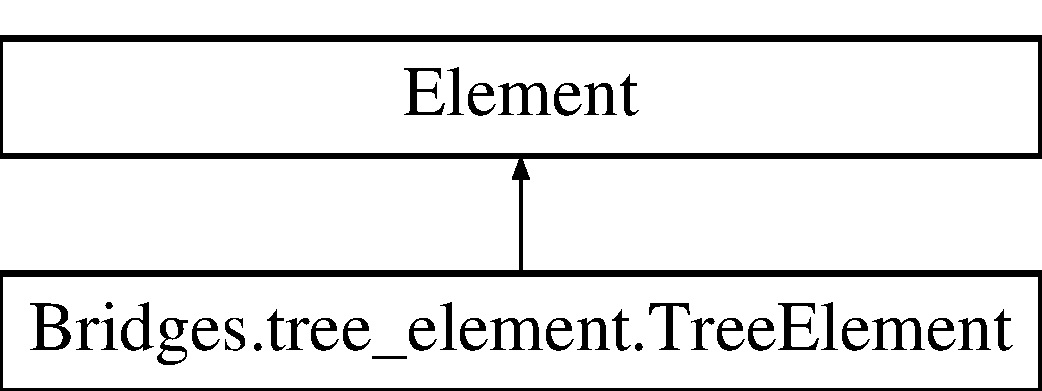
\includegraphics[height=2.000000cm]{class_bridges_1_1tree__element_1_1_tree_element}
\end{center}
\end{figure}
\subsection*{Public Member Functions}
\begin{DoxyCompactItemize}
\item 
def \mbox{\hyperlink{class_bridges_1_1tree__element_1_1_tree_element_a62b157ce953614dc9ac28b5361c3febf}{\+\_\+\+\_\+init\+\_\+\+\_\+}} (self, label=None, e=None, left=None, right=None)
\begin{DoxyCompactList}\small\item\em Constructs an \mbox{\hyperlink{class_bridges_1_1tree__element_1_1_tree_element}{Tree\+Element}} set to null. \end{DoxyCompactList}\item 
def \mbox{\hyperlink{class_bridges_1_1tree__element_1_1_tree_element_a943d5ba52e289152f700fad7650bfc18}{get\+\_\+data\+\_\+structure\+\_\+type}} (self)
\begin{DoxyCompactList}\small\item\em This method gets the data structure type. \end{DoxyCompactList}\item 
def \mbox{\hyperlink{class_bridges_1_1tree__element_1_1_tree_element_a5cc7c317f44d0c19e76f05ed70b78bb4}{add\+\_\+child}} (self, child)
\begin{DoxyCompactList}\small\item\em Adds a child to the node. \end{DoxyCompactList}\item 
def \mbox{\hyperlink{class_bridges_1_1tree__element_1_1_tree_element_a10d73cf3beac493c8ea835326fd0d84b}{get\+\_\+number\+\_\+of\+\_\+children}} (self)
\begin{DoxyCompactList}\small\item\em Returns the number of children at this node. \end{DoxyCompactList}\item 
def \mbox{\hyperlink{class_bridges_1_1tree__element_1_1_tree_element_af6bb2b4b836002c3ebdf0fda35251df5}{set\+\_\+child}} (self, index, child)
\begin{DoxyCompactList}\small\item\em adds a child to the node -\/ will be added at the next open position \end{DoxyCompactList}\item 
def \mbox{\hyperlink{class_bridges_1_1tree__element_1_1_tree_element_a637130167474ec5ddffd62652fab2abb}{get\+\_\+child}} (self, index)
\begin{DoxyCompactList}\small\item\em gets a child at a particular index \end{DoxyCompactList}\item 
def \mbox{\hyperlink{class_bridges_1_1tree__element_1_1_tree_element_a080c9c808fc5fe3b551ed6eae276d168}{get\+\_\+data\+\_\+structure\+\_\+representation}} (self)
\begin{DoxyCompactList}\small\item\em Get hierarchical J\+S\+ON of the tree representation. \end{DoxyCompactList}\item 
def \mbox{\hyperlink{class_bridges_1_1tree__element_1_1_tree_element_a4b036840b8ba63d789a94d9a68c2aa75}{pre\+\_\+order}} (self, root)
\begin{DoxyCompactList}\small\item\em Use a preorder traversal to directly extract a hierarchical J\+S\+ON representation of the tree. \end{DoxyCompactList}\end{DoxyCompactItemize}
\subsection*{Public Attributes}
\begin{DoxyCompactItemize}
\item 
\mbox{\hyperlink{class_bridges_1_1tree__element_1_1_tree_element_a8857c49f462f75b3f8b4ff4296948420}{children}}
\end{DoxyCompactItemize}
\subsection*{Static Public Attributes}
\begin{DoxyCompactItemize}
\item 
list \mbox{\hyperlink{class_bridges_1_1tree__element_1_1_tree_element_ae60bd5a03a4dcfb9cbc75d0f990afc09}{children}} = \mbox{[}$\,$\mbox{]}
\item 
string \mbox{\hyperlink{class_bridges_1_1tree__element_1_1_tree_element_af14308b7ca08bea361da3578def2fbd3}{Q\+U\+O\+TE}} = \char`\"{}\textbackslash{}\char`\"{}\char`\"{}
\item 
string \mbox{\hyperlink{class_bridges_1_1tree__element_1_1_tree_element_a86ddb269cd60bbebdeb19ceda3e3b364}{C\+O\+M\+MA}} = \char`\"{},\char`\"{}
\item 
string \mbox{\hyperlink{class_bridges_1_1tree__element_1_1_tree_element_afdd07830c301e15c61c30b02ddce845f}{C\+O\+L\+ON}} = \char`\"{}\+:\char`\"{}
\item 
string \mbox{\hyperlink{class_bridges_1_1tree__element_1_1_tree_element_a7eaef303a46a18faa572f54c9f5bb956}{O\+P\+E\+N\+\_\+\+C\+U\+R\+LY}} = \char`\"{}\{\char`\"{}
\item 
string \mbox{\hyperlink{class_bridges_1_1tree__element_1_1_tree_element_ac12400eb161e8402ede3c69c231d8fe4}{C\+L\+O\+S\+E\+\_\+\+C\+U\+R\+LY}} = \char`\"{}\}\char`\"{}
\item 
string \mbox{\hyperlink{class_bridges_1_1tree__element_1_1_tree_element_af79b871189bd339d5f7e9d49c4eac947}{O\+P\+E\+N\+\_\+\+P\+A\+R\+EN}} = \char`\"{}(\char`\"{}
\item 
string \mbox{\hyperlink{class_bridges_1_1tree__element_1_1_tree_element_a7d36a749d78f10cfa6057c1ffba1b6d8}{C\+L\+O\+S\+E\+\_\+\+P\+A\+R\+EN}} = \char`\"{})\char`\"{}
\item 
string \mbox{\hyperlink{class_bridges_1_1tree__element_1_1_tree_element_a171eccb97594115dfdf80f835561c0eb}{O\+P\+E\+N\+\_\+\+B\+OX}} = \char`\"{}\mbox{[}\char`\"{}
\item 
string \mbox{\hyperlink{class_bridges_1_1tree__element_1_1_tree_element_a87b30ef7a835013a12af51f1469b24e3}{C\+L\+O\+S\+E\+\_\+\+B\+OX}} = \char`\"{}\mbox{]}\char`\"{}
\end{DoxyCompactItemize}


\subsection{Detailed Description}
This class extends Element to represent general trees with arbitrary number of children. 

\mbox{\hyperlink{class_bridges_1_1tree__element_1_1_tree_element}{Tree\+Element}} nodes can have an arbitrary number of child nodes(held in in a vector in the order in which they were added). The visualization of trees assumes that the children are drawn in order from left to right.

Tree Elements have labels (string) that are displayed on the visualization. Elements take an generic object E as a user defined parameter, which can be any native type or object.

Elements contain a visualizer (Element\+Visualizer) object for setting visual attributes (color, shape, opacity, size), necessary for displaying them in a web browser.

Elements also have a Link\+Visualizer object that is used when they are linked to another element, appropriate for setting link attributes, between parent and child nodes.

\begin{DoxyAuthor}{Author}
Matthew Mc\+Quaigue 
\end{DoxyAuthor}


\subsection{Constructor \& Destructor Documentation}
\mbox{\Hypertarget{class_bridges_1_1tree__element_1_1_tree_element_a62b157ce953614dc9ac28b5361c3febf}\label{class_bridges_1_1tree__element_1_1_tree_element_a62b157ce953614dc9ac28b5361c3febf}} 
\index{Bridges\+::tree\+\_\+element\+::\+Tree\+Element@{Bridges\+::tree\+\_\+element\+::\+Tree\+Element}!\+\_\+\+\_\+init\+\_\+\+\_\+@{\+\_\+\+\_\+init\+\_\+\+\_\+}}
\index{\+\_\+\+\_\+init\+\_\+\+\_\+@{\+\_\+\+\_\+init\+\_\+\+\_\+}!Bridges\+::tree\+\_\+element\+::\+Tree\+Element@{Bridges\+::tree\+\_\+element\+::\+Tree\+Element}}
\subsubsection{\texorpdfstring{\+\_\+\+\_\+init\+\_\+\+\_\+()}{\_\_init\_\_()}}
{\footnotesize\ttfamily def Bridges.\+tree\+\_\+element.\+Tree\+Element.\+\_\+\+\_\+init\+\_\+\+\_\+ (\begin{DoxyParamCaption}\item[{}]{self,  }\item[{}]{label = {\ttfamily None},  }\item[{}]{e = {\ttfamily None},  }\item[{}]{left = {\ttfamily None},  }\item[{}]{right = {\ttfamily None} }\end{DoxyParamCaption})}



Constructs an \mbox{\hyperlink{class_bridges_1_1tree__element_1_1_tree_element}{Tree\+Element}} set to null. 


\begin{DoxyParams}{Parameters}
{\em e} & the generic object that \mbox{\hyperlink{class_bridges_1_1tree__element_1_1_tree_element}{Tree\+Element}} will hold \\
\hline
{\em label} & the label of \mbox{\hyperlink{class_bridges_1_1tree__element_1_1_tree_element}{Tree\+Element}} that shows up on the bridges \\
\hline
{\em left} & the \mbox{\hyperlink{class_bridges_1_1tree__element_1_1_tree_element}{Tree\+Element}} to be assigned to the child 0 \\
\hline
{\em right} & the \mbox{\hyperlink{class_bridges_1_1tree__element_1_1_tree_element}{Tree\+Element}} to be assigned to the child 1 \\
\hline
\end{DoxyParams}


\subsection{Member Function Documentation}
\mbox{\Hypertarget{class_bridges_1_1tree__element_1_1_tree_element_a5cc7c317f44d0c19e76f05ed70b78bb4}\label{class_bridges_1_1tree__element_1_1_tree_element_a5cc7c317f44d0c19e76f05ed70b78bb4}} 
\index{Bridges\+::tree\+\_\+element\+::\+Tree\+Element@{Bridges\+::tree\+\_\+element\+::\+Tree\+Element}!add\+\_\+child@{add\+\_\+child}}
\index{add\+\_\+child@{add\+\_\+child}!Bridges\+::tree\+\_\+element\+::\+Tree\+Element@{Bridges\+::tree\+\_\+element\+::\+Tree\+Element}}
\subsubsection{\texorpdfstring{add\+\_\+child()}{add\_child()}}
{\footnotesize\ttfamily def Bridges.\+tree\+\_\+element.\+Tree\+Element.\+add\+\_\+child (\begin{DoxyParamCaption}\item[{}]{self,  }\item[{}]{child }\end{DoxyParamCaption})}



Adds a child to the node. 

\mbox{\Hypertarget{class_bridges_1_1tree__element_1_1_tree_element_a637130167474ec5ddffd62652fab2abb}\label{class_bridges_1_1tree__element_1_1_tree_element_a637130167474ec5ddffd62652fab2abb}} 
\index{Bridges\+::tree\+\_\+element\+::\+Tree\+Element@{Bridges\+::tree\+\_\+element\+::\+Tree\+Element}!get\+\_\+child@{get\+\_\+child}}
\index{get\+\_\+child@{get\+\_\+child}!Bridges\+::tree\+\_\+element\+::\+Tree\+Element@{Bridges\+::tree\+\_\+element\+::\+Tree\+Element}}
\subsubsection{\texorpdfstring{get\+\_\+child()}{get\_child()}}
{\footnotesize\ttfamily def Bridges.\+tree\+\_\+element.\+Tree\+Element.\+get\+\_\+child (\begin{DoxyParamCaption}\item[{}]{self,  }\item[{}]{index }\end{DoxyParamCaption})}



gets a child at a particular index 


\begin{DoxyParams}{Parameters}
{\em index} & into the list of children\\
\hline
\end{DoxyParams}
\begin{DoxyReturn}{Returns}
child to be returned 
\end{DoxyReturn}
\mbox{\Hypertarget{class_bridges_1_1tree__element_1_1_tree_element_a080c9c808fc5fe3b551ed6eae276d168}\label{class_bridges_1_1tree__element_1_1_tree_element_a080c9c808fc5fe3b551ed6eae276d168}} 
\index{Bridges\+::tree\+\_\+element\+::\+Tree\+Element@{Bridges\+::tree\+\_\+element\+::\+Tree\+Element}!get\+\_\+data\+\_\+structure\+\_\+representation@{get\+\_\+data\+\_\+structure\+\_\+representation}}
\index{get\+\_\+data\+\_\+structure\+\_\+representation@{get\+\_\+data\+\_\+structure\+\_\+representation}!Bridges\+::tree\+\_\+element\+::\+Tree\+Element@{Bridges\+::tree\+\_\+element\+::\+Tree\+Element}}
\subsubsection{\texorpdfstring{get\+\_\+data\+\_\+structure\+\_\+representation()}{get\_data\_structure\_representation()}}
{\footnotesize\ttfamily def Bridges.\+tree\+\_\+element.\+Tree\+Element.\+get\+\_\+data\+\_\+structure\+\_\+representation (\begin{DoxyParamCaption}\item[{}]{self }\end{DoxyParamCaption})}



Get hierarchical J\+S\+ON of the tree representation. 

\begin{DoxyReturn}{Returns}
the J\+S\+ON string 
\end{DoxyReturn}
\mbox{\Hypertarget{class_bridges_1_1tree__element_1_1_tree_element_a943d5ba52e289152f700fad7650bfc18}\label{class_bridges_1_1tree__element_1_1_tree_element_a943d5ba52e289152f700fad7650bfc18}} 
\index{Bridges\+::tree\+\_\+element\+::\+Tree\+Element@{Bridges\+::tree\+\_\+element\+::\+Tree\+Element}!get\+\_\+data\+\_\+structure\+\_\+type@{get\+\_\+data\+\_\+structure\+\_\+type}}
\index{get\+\_\+data\+\_\+structure\+\_\+type@{get\+\_\+data\+\_\+structure\+\_\+type}!Bridges\+::tree\+\_\+element\+::\+Tree\+Element@{Bridges\+::tree\+\_\+element\+::\+Tree\+Element}}
\subsubsection{\texorpdfstring{get\+\_\+data\+\_\+structure\+\_\+type()}{get\_data\_structure\_type()}}
{\footnotesize\ttfamily def Bridges.\+tree\+\_\+element.\+Tree\+Element.\+get\+\_\+data\+\_\+structure\+\_\+type (\begin{DoxyParamCaption}\item[{}]{self }\end{DoxyParamCaption})}



This method gets the data structure type. 

\begin{DoxyReturn}{Returns}
The date structure type as a string 
\end{DoxyReturn}
\mbox{\Hypertarget{class_bridges_1_1tree__element_1_1_tree_element_a10d73cf3beac493c8ea835326fd0d84b}\label{class_bridges_1_1tree__element_1_1_tree_element_a10d73cf3beac493c8ea835326fd0d84b}} 
\index{Bridges\+::tree\+\_\+element\+::\+Tree\+Element@{Bridges\+::tree\+\_\+element\+::\+Tree\+Element}!get\+\_\+number\+\_\+of\+\_\+children@{get\+\_\+number\+\_\+of\+\_\+children}}
\index{get\+\_\+number\+\_\+of\+\_\+children@{get\+\_\+number\+\_\+of\+\_\+children}!Bridges\+::tree\+\_\+element\+::\+Tree\+Element@{Bridges\+::tree\+\_\+element\+::\+Tree\+Element}}
\subsubsection{\texorpdfstring{get\+\_\+number\+\_\+of\+\_\+children()}{get\_number\_of\_children()}}
{\footnotesize\ttfamily def Bridges.\+tree\+\_\+element.\+Tree\+Element.\+get\+\_\+number\+\_\+of\+\_\+children (\begin{DoxyParamCaption}\item[{}]{self }\end{DoxyParamCaption})}



Returns the number of children at this node. 

\begin{DoxyReturn}{Returns}
number of children 
\end{DoxyReturn}
\mbox{\Hypertarget{class_bridges_1_1tree__element_1_1_tree_element_a4b036840b8ba63d789a94d9a68c2aa75}\label{class_bridges_1_1tree__element_1_1_tree_element_a4b036840b8ba63d789a94d9a68c2aa75}} 
\index{Bridges\+::tree\+\_\+element\+::\+Tree\+Element@{Bridges\+::tree\+\_\+element\+::\+Tree\+Element}!pre\+\_\+order@{pre\+\_\+order}}
\index{pre\+\_\+order@{pre\+\_\+order}!Bridges\+::tree\+\_\+element\+::\+Tree\+Element@{Bridges\+::tree\+\_\+element\+::\+Tree\+Element}}
\subsubsection{\texorpdfstring{pre\+\_\+order()}{pre\_order()}}
{\footnotesize\ttfamily def Bridges.\+tree\+\_\+element.\+Tree\+Element.\+pre\+\_\+order (\begin{DoxyParamCaption}\item[{}]{self,  }\item[{}]{root }\end{DoxyParamCaption})}



Use a preorder traversal to directly extract a hierarchical J\+S\+ON representation of the tree. 

\mbox{\Hypertarget{class_bridges_1_1tree__element_1_1_tree_element_af6bb2b4b836002c3ebdf0fda35251df5}\label{class_bridges_1_1tree__element_1_1_tree_element_af6bb2b4b836002c3ebdf0fda35251df5}} 
\index{Bridges\+::tree\+\_\+element\+::\+Tree\+Element@{Bridges\+::tree\+\_\+element\+::\+Tree\+Element}!set\+\_\+child@{set\+\_\+child}}
\index{set\+\_\+child@{set\+\_\+child}!Bridges\+::tree\+\_\+element\+::\+Tree\+Element@{Bridges\+::tree\+\_\+element\+::\+Tree\+Element}}
\subsubsection{\texorpdfstring{set\+\_\+child()}{set\_child()}}
{\footnotesize\ttfamily def Bridges.\+tree\+\_\+element.\+Tree\+Element.\+set\+\_\+child (\begin{DoxyParamCaption}\item[{}]{self,  }\item[{}]{index,  }\item[{}]{child }\end{DoxyParamCaption})}



adds a child to the node -\/ will be added at the next open position 


\begin{DoxyParams}{Parameters}
{\em child} & to be added\\
\hline
\end{DoxyParams}
\begin{DoxyReturn}{Returns}
none 
\end{DoxyReturn}


\subsection{Member Data Documentation}
\mbox{\Hypertarget{class_bridges_1_1tree__element_1_1_tree_element_ae60bd5a03a4dcfb9cbc75d0f990afc09}\label{class_bridges_1_1tree__element_1_1_tree_element_ae60bd5a03a4dcfb9cbc75d0f990afc09}} 
\index{Bridges\+::tree\+\_\+element\+::\+Tree\+Element@{Bridges\+::tree\+\_\+element\+::\+Tree\+Element}!children@{children}}
\index{children@{children}!Bridges\+::tree\+\_\+element\+::\+Tree\+Element@{Bridges\+::tree\+\_\+element\+::\+Tree\+Element}}
\subsubsection{\texorpdfstring{children}{children}\hspace{0.1cm}{\footnotesize\ttfamily [1/2]}}
{\footnotesize\ttfamily list Bridges.\+tree\+\_\+element.\+Tree\+Element.\+children = \mbox{[}$\,$\mbox{]}\hspace{0.3cm}{\ttfamily [static]}}

\mbox{\Hypertarget{class_bridges_1_1tree__element_1_1_tree_element_a8857c49f462f75b3f8b4ff4296948420}\label{class_bridges_1_1tree__element_1_1_tree_element_a8857c49f462f75b3f8b4ff4296948420}} 
\index{Bridges\+::tree\+\_\+element\+::\+Tree\+Element@{Bridges\+::tree\+\_\+element\+::\+Tree\+Element}!children@{children}}
\index{children@{children}!Bridges\+::tree\+\_\+element\+::\+Tree\+Element@{Bridges\+::tree\+\_\+element\+::\+Tree\+Element}}
\subsubsection{\texorpdfstring{children}{children}\hspace{0.1cm}{\footnotesize\ttfamily [2/2]}}
{\footnotesize\ttfamily Bridges.\+tree\+\_\+element.\+Tree\+Element.\+children}

\mbox{\Hypertarget{class_bridges_1_1tree__element_1_1_tree_element_a87b30ef7a835013a12af51f1469b24e3}\label{class_bridges_1_1tree__element_1_1_tree_element_a87b30ef7a835013a12af51f1469b24e3}} 
\index{Bridges\+::tree\+\_\+element\+::\+Tree\+Element@{Bridges\+::tree\+\_\+element\+::\+Tree\+Element}!C\+L\+O\+S\+E\+\_\+\+B\+OX@{C\+L\+O\+S\+E\+\_\+\+B\+OX}}
\index{C\+L\+O\+S\+E\+\_\+\+B\+OX@{C\+L\+O\+S\+E\+\_\+\+B\+OX}!Bridges\+::tree\+\_\+element\+::\+Tree\+Element@{Bridges\+::tree\+\_\+element\+::\+Tree\+Element}}
\subsubsection{\texorpdfstring{C\+L\+O\+S\+E\+\_\+\+B\+OX}{CLOSE\_BOX}}
{\footnotesize\ttfamily string Bridges.\+tree\+\_\+element.\+Tree\+Element.\+C\+L\+O\+S\+E\+\_\+\+B\+OX = \char`\"{}\mbox{]}\char`\"{}\hspace{0.3cm}{\ttfamily [static]}}

\mbox{\Hypertarget{class_bridges_1_1tree__element_1_1_tree_element_ac12400eb161e8402ede3c69c231d8fe4}\label{class_bridges_1_1tree__element_1_1_tree_element_ac12400eb161e8402ede3c69c231d8fe4}} 
\index{Bridges\+::tree\+\_\+element\+::\+Tree\+Element@{Bridges\+::tree\+\_\+element\+::\+Tree\+Element}!C\+L\+O\+S\+E\+\_\+\+C\+U\+R\+LY@{C\+L\+O\+S\+E\+\_\+\+C\+U\+R\+LY}}
\index{C\+L\+O\+S\+E\+\_\+\+C\+U\+R\+LY@{C\+L\+O\+S\+E\+\_\+\+C\+U\+R\+LY}!Bridges\+::tree\+\_\+element\+::\+Tree\+Element@{Bridges\+::tree\+\_\+element\+::\+Tree\+Element}}
\subsubsection{\texorpdfstring{C\+L\+O\+S\+E\+\_\+\+C\+U\+R\+LY}{CLOSE\_CURLY}}
{\footnotesize\ttfamily string Bridges.\+tree\+\_\+element.\+Tree\+Element.\+C\+L\+O\+S\+E\+\_\+\+C\+U\+R\+LY = \char`\"{}\}\char`\"{}\hspace{0.3cm}{\ttfamily [static]}}

\mbox{\Hypertarget{class_bridges_1_1tree__element_1_1_tree_element_a7d36a749d78f10cfa6057c1ffba1b6d8}\label{class_bridges_1_1tree__element_1_1_tree_element_a7d36a749d78f10cfa6057c1ffba1b6d8}} 
\index{Bridges\+::tree\+\_\+element\+::\+Tree\+Element@{Bridges\+::tree\+\_\+element\+::\+Tree\+Element}!C\+L\+O\+S\+E\+\_\+\+P\+A\+R\+EN@{C\+L\+O\+S\+E\+\_\+\+P\+A\+R\+EN}}
\index{C\+L\+O\+S\+E\+\_\+\+P\+A\+R\+EN@{C\+L\+O\+S\+E\+\_\+\+P\+A\+R\+EN}!Bridges\+::tree\+\_\+element\+::\+Tree\+Element@{Bridges\+::tree\+\_\+element\+::\+Tree\+Element}}
\subsubsection{\texorpdfstring{C\+L\+O\+S\+E\+\_\+\+P\+A\+R\+EN}{CLOSE\_PAREN}}
{\footnotesize\ttfamily string Bridges.\+tree\+\_\+element.\+Tree\+Element.\+C\+L\+O\+S\+E\+\_\+\+P\+A\+R\+EN = \char`\"{})\char`\"{}\hspace{0.3cm}{\ttfamily [static]}}

\mbox{\Hypertarget{class_bridges_1_1tree__element_1_1_tree_element_afdd07830c301e15c61c30b02ddce845f}\label{class_bridges_1_1tree__element_1_1_tree_element_afdd07830c301e15c61c30b02ddce845f}} 
\index{Bridges\+::tree\+\_\+element\+::\+Tree\+Element@{Bridges\+::tree\+\_\+element\+::\+Tree\+Element}!C\+O\+L\+ON@{C\+O\+L\+ON}}
\index{C\+O\+L\+ON@{C\+O\+L\+ON}!Bridges\+::tree\+\_\+element\+::\+Tree\+Element@{Bridges\+::tree\+\_\+element\+::\+Tree\+Element}}
\subsubsection{\texorpdfstring{C\+O\+L\+ON}{COLON}}
{\footnotesize\ttfamily string Bridges.\+tree\+\_\+element.\+Tree\+Element.\+C\+O\+L\+ON = \char`\"{}\+:\char`\"{}\hspace{0.3cm}{\ttfamily [static]}}

\mbox{\Hypertarget{class_bridges_1_1tree__element_1_1_tree_element_a86ddb269cd60bbebdeb19ceda3e3b364}\label{class_bridges_1_1tree__element_1_1_tree_element_a86ddb269cd60bbebdeb19ceda3e3b364}} 
\index{Bridges\+::tree\+\_\+element\+::\+Tree\+Element@{Bridges\+::tree\+\_\+element\+::\+Tree\+Element}!C\+O\+M\+MA@{C\+O\+M\+MA}}
\index{C\+O\+M\+MA@{C\+O\+M\+MA}!Bridges\+::tree\+\_\+element\+::\+Tree\+Element@{Bridges\+::tree\+\_\+element\+::\+Tree\+Element}}
\subsubsection{\texorpdfstring{C\+O\+M\+MA}{COMMA}}
{\footnotesize\ttfamily string Bridges.\+tree\+\_\+element.\+Tree\+Element.\+C\+O\+M\+MA = \char`\"{},\char`\"{}\hspace{0.3cm}{\ttfamily [static]}}

\mbox{\Hypertarget{class_bridges_1_1tree__element_1_1_tree_element_a171eccb97594115dfdf80f835561c0eb}\label{class_bridges_1_1tree__element_1_1_tree_element_a171eccb97594115dfdf80f835561c0eb}} 
\index{Bridges\+::tree\+\_\+element\+::\+Tree\+Element@{Bridges\+::tree\+\_\+element\+::\+Tree\+Element}!O\+P\+E\+N\+\_\+\+B\+OX@{O\+P\+E\+N\+\_\+\+B\+OX}}
\index{O\+P\+E\+N\+\_\+\+B\+OX@{O\+P\+E\+N\+\_\+\+B\+OX}!Bridges\+::tree\+\_\+element\+::\+Tree\+Element@{Bridges\+::tree\+\_\+element\+::\+Tree\+Element}}
\subsubsection{\texorpdfstring{O\+P\+E\+N\+\_\+\+B\+OX}{OPEN\_BOX}}
{\footnotesize\ttfamily string Bridges.\+tree\+\_\+element.\+Tree\+Element.\+O\+P\+E\+N\+\_\+\+B\+OX = \char`\"{}\mbox{[}\char`\"{}\hspace{0.3cm}{\ttfamily [static]}}

\mbox{\Hypertarget{class_bridges_1_1tree__element_1_1_tree_element_a7eaef303a46a18faa572f54c9f5bb956}\label{class_bridges_1_1tree__element_1_1_tree_element_a7eaef303a46a18faa572f54c9f5bb956}} 
\index{Bridges\+::tree\+\_\+element\+::\+Tree\+Element@{Bridges\+::tree\+\_\+element\+::\+Tree\+Element}!O\+P\+E\+N\+\_\+\+C\+U\+R\+LY@{O\+P\+E\+N\+\_\+\+C\+U\+R\+LY}}
\index{O\+P\+E\+N\+\_\+\+C\+U\+R\+LY@{O\+P\+E\+N\+\_\+\+C\+U\+R\+LY}!Bridges\+::tree\+\_\+element\+::\+Tree\+Element@{Bridges\+::tree\+\_\+element\+::\+Tree\+Element}}
\subsubsection{\texorpdfstring{O\+P\+E\+N\+\_\+\+C\+U\+R\+LY}{OPEN\_CURLY}}
{\footnotesize\ttfamily string Bridges.\+tree\+\_\+element.\+Tree\+Element.\+O\+P\+E\+N\+\_\+\+C\+U\+R\+LY = \char`\"{}\{\char`\"{}\hspace{0.3cm}{\ttfamily [static]}}

\mbox{\Hypertarget{class_bridges_1_1tree__element_1_1_tree_element_af79b871189bd339d5f7e9d49c4eac947}\label{class_bridges_1_1tree__element_1_1_tree_element_af79b871189bd339d5f7e9d49c4eac947}} 
\index{Bridges\+::tree\+\_\+element\+::\+Tree\+Element@{Bridges\+::tree\+\_\+element\+::\+Tree\+Element}!O\+P\+E\+N\+\_\+\+P\+A\+R\+EN@{O\+P\+E\+N\+\_\+\+P\+A\+R\+EN}}
\index{O\+P\+E\+N\+\_\+\+P\+A\+R\+EN@{O\+P\+E\+N\+\_\+\+P\+A\+R\+EN}!Bridges\+::tree\+\_\+element\+::\+Tree\+Element@{Bridges\+::tree\+\_\+element\+::\+Tree\+Element}}
\subsubsection{\texorpdfstring{O\+P\+E\+N\+\_\+\+P\+A\+R\+EN}{OPEN\_PAREN}}
{\footnotesize\ttfamily string Bridges.\+tree\+\_\+element.\+Tree\+Element.\+O\+P\+E\+N\+\_\+\+P\+A\+R\+EN = \char`\"{}(\char`\"{}\hspace{0.3cm}{\ttfamily [static]}}

\mbox{\Hypertarget{class_bridges_1_1tree__element_1_1_tree_element_af14308b7ca08bea361da3578def2fbd3}\label{class_bridges_1_1tree__element_1_1_tree_element_af14308b7ca08bea361da3578def2fbd3}} 
\index{Bridges\+::tree\+\_\+element\+::\+Tree\+Element@{Bridges\+::tree\+\_\+element\+::\+Tree\+Element}!Q\+U\+O\+TE@{Q\+U\+O\+TE}}
\index{Q\+U\+O\+TE@{Q\+U\+O\+TE}!Bridges\+::tree\+\_\+element\+::\+Tree\+Element@{Bridges\+::tree\+\_\+element\+::\+Tree\+Element}}
\subsubsection{\texorpdfstring{Q\+U\+O\+TE}{QUOTE}}
{\footnotesize\ttfamily string Bridges.\+tree\+\_\+element.\+Tree\+Element.\+Q\+U\+O\+TE = \char`\"{}\textbackslash{}\char`\"{}\char`\"{}\hspace{0.3cm}{\ttfamily [static]}}



The documentation for this class was generated from the following file\+:\begin{DoxyCompactItemize}
\item 
/\+Users/kalpathi/gr/bridges/client/python/bridges18/\+Bridges/\mbox{\hyperlink{tree__element_8py}{tree\+\_\+element.\+py}}\end{DoxyCompactItemize}

\chapter{File Documentation}
\hypertarget{____init_____8py}{}\section{/\+Users/krs/pysrc/\+Bridges/\+\_\+\+\_\+init\+\_\+\+\_\+.py File Reference}
\label{____init_____8py}\index{/\+Users/krs/pysrc/\+Bridges/\+\_\+\+\_\+init\+\_\+\+\_\+.\+py@{/\+Users/krs/pysrc/\+Bridges/\+\_\+\+\_\+init\+\_\+\+\_\+.\+py}}
\subsection*{Namespaces}
\begin{DoxyCompactItemize}
\item 
 \hyperlink{namespace_bridges}{Bridges}
\end{DoxyCompactItemize}

\hypertarget{array_8py}{}\section{/\+Users/kalpathi/gr/bridges/client/python/bridges/array.py File Reference}
\label{array_8py}\index{/\+Users/kalpathi/gr/bridges/client/python/bridges/array.\+py@{/\+Users/kalpathi/gr/bridges/client/python/bridges/array.\+py}}
\subsection*{Classes}
\begin{DoxyCompactItemize}
\item 
class \hyperlink{classbridges_1_1array_1_1_array}{bridges.\+array.\+Array}
\begin{DoxyCompactList}\small\item\em This class can be used to create arrays of type Element$<$\+E$>$. \end{DoxyCompactList}\end{DoxyCompactItemize}
\subsection*{Namespaces}
\begin{DoxyCompactItemize}
\item 
 \hyperlink{namespacebridges_1_1array}{bridges.\+array}
\end{DoxyCompactItemize}

\hypertarget{avl__tree__element_8py}{}\section{/\+Users/kalpathi/gr/bridges/python/bridges/avl\+\_\+tree\+\_\+element.py File Reference}
\label{avl__tree__element_8py}\index{/Users/kalpathi/gr/bridges/python/bridges/avl\_tree\_element.py@{/Users/kalpathi/gr/bridges/python/bridges/avl\_tree\_element.py}}
\subsection*{Classes}
\begin{DoxyCompactItemize}
\item 
class \mbox{\hyperlink{classbridges_1_1avl__tree__element_1_1_a_v_l_tree_element}{bridges.\+avl\+\_\+tree\+\_\+element.\+A\+V\+L\+Tree\+Element}}
\begin{DoxyCompactList}\small\item\em This class extends the B\+S\+T\+Element class by adding a height and balance factor fields that are useful in A\+VL trees. \end{DoxyCompactList}\end{DoxyCompactItemize}
\subsection*{Namespaces}
\begin{DoxyCompactItemize}
\item 
 \mbox{\hyperlink{namespacebridges_1_1avl__tree__element}{bridges.\+avl\+\_\+tree\+\_\+element}}
\end{DoxyCompactItemize}

\hypertarget{bin__tree__element_8py}{}\section{/\+Users/kalpathi/gr/bridges/client/python/bridges18/\+Bridges/bin\+\_\+tree\+\_\+element.py File Reference}
\label{bin__tree__element_8py}\index{/\+Users/kalpathi/gr/bridges/client/python/bridges18/\+Bridges/bin\+\_\+tree\+\_\+element.\+py@{/\+Users/kalpathi/gr/bridges/client/python/bridges18/\+Bridges/bin\+\_\+tree\+\_\+element.\+py}}
\subsection*{Classes}
\begin{DoxyCompactItemize}
\item 
class \mbox{\hyperlink{class_bridges_1_1bin__tree__element_1_1_bin_tree_element}{Bridges.\+bin\+\_\+tree\+\_\+element.\+Bin\+Tree\+Element}}
\begin{DoxyCompactList}\small\item\em This class is extended from the Tree\+Element class and can be used to create binary tree element objects. \end{DoxyCompactList}\end{DoxyCompactItemize}
\subsection*{Namespaces}
\begin{DoxyCompactItemize}
\item 
 \mbox{\hyperlink{namespace_bridges_1_1bin__tree__element}{Bridges.\+bin\+\_\+tree\+\_\+element}}
\end{DoxyCompactItemize}

\hypertarget{bridges_8py}{}\section{/\+Users/kalpathi/gr/bridges/python/bridges/bridges.py File Reference}
\label{bridges_8py}\index{/Users/kalpathi/gr/bridges/python/bridges/bridges.py@{/Users/kalpathi/gr/bridges/python/bridges/bridges.py}}
\subsection*{Classes}
\begin{DoxyCompactItemize}
\item 
class \mbox{\hyperlink{classbridges_1_1bridges_1_1_bridges}{bridges.\+bridges.\+Bridges}}
\begin{DoxyCompactList}\small\item\em The bridges class is the main class that provides interfaces to datasets, maintains user and assignment information, and connects to the bridges server. \end{DoxyCompactList}\end{DoxyCompactItemize}
\subsection*{Namespaces}
\begin{DoxyCompactItemize}
\item 
 \mbox{\hyperlink{namespacebridges_1_1bridges}{bridges.\+bridges}}
\end{DoxyCompactItemize}

\hypertarget{bst__element_8py}{}\section{/home/erik/work/bridges/bridges-\/python/bridges/bst\+\_\+element.py File Reference}
\label{bst__element_8py}\index{/home/erik/work/bridges/bridges-\/python/bridges/bst\+\_\+element.\+py@{/home/erik/work/bridges/bridges-\/python/bridges/bst\+\_\+element.\+py}}
\subsection*{Classes}
\begin{DoxyCompactItemize}
\item 
class \hyperlink{classbridges_1_1bst__element_1_1_b_s_t_element}{bridges.\+bst\+\_\+element.\+B\+S\+T\+Element}
\begin{DoxyCompactList}\small\item\em The \hyperlink{classbridges_1_1bst__element_1_1_b_s_t_element}{B\+S\+T\+Element} class is the building block for creating binary search trees. \end{DoxyCompactList}\end{DoxyCompactItemize}
\subsection*{Namespaces}
\begin{DoxyCompactItemize}
\item 
 \hyperlink{namespacebridges_1_1bst__element}{bridges.\+bst\+\_\+element}
\end{DoxyCompactItemize}

\hypertarget{circ__dl__element_8py}{}\section{/home/erik/work/bridges/bridges-\/python/bridges/circ\+\_\+dl\+\_\+element.py File Reference}
\label{circ__dl__element_8py}\index{/home/erik/work/bridges/bridges-\/python/bridges/circ\+\_\+dl\+\_\+element.\+py@{/home/erik/work/bridges/bridges-\/python/bridges/circ\+\_\+dl\+\_\+element.\+py}}
\subsection*{Classes}
\begin{DoxyCompactItemize}
\item 
class \hyperlink{classbridges_1_1circ__dl__element_1_1_circ_d_lelement}{bridges.\+circ\+\_\+dl\+\_\+element.\+Circ\+D\+Lelement}
\begin{DoxyCompactList}\small\item\em This class can be used to instantiate Circular Doubly Linked List Elements. \end{DoxyCompactList}\end{DoxyCompactItemize}
\subsection*{Namespaces}
\begin{DoxyCompactItemize}
\item 
 \hyperlink{namespacebridges_1_1circ__dl__element}{bridges.\+circ\+\_\+dl\+\_\+element}
\end{DoxyCompactItemize}

\hypertarget{circ__sl__element_8py}{}\section{/home/erik/work/bridges/bridges-\/python/bridges/circ\+\_\+sl\+\_\+element.py File Reference}
\label{circ__sl__element_8py}\index{/home/erik/work/bridges/bridges-\/python/bridges/circ\+\_\+sl\+\_\+element.\+py@{/home/erik/work/bridges/bridges-\/python/bridges/circ\+\_\+sl\+\_\+element.\+py}}
\subsection*{Classes}
\begin{DoxyCompactItemize}
\item 
class \hyperlink{classbridges_1_1circ__sl__element_1_1_circ_s_lelement}{bridges.\+circ\+\_\+sl\+\_\+element.\+Circ\+S\+Lelement}
\begin{DoxyCompactList}\small\item\em This class can be used to instantiate Singly Linked Circular List Elements. \end{DoxyCompactList}\item 
class \hyperlink{classbridges_1_1circ__sl__element_1_1_circ_slelement_iterator}{bridges.\+circ\+\_\+sl\+\_\+element.\+Circ\+Slelement\+Iterator}
\end{DoxyCompactItemize}
\subsection*{Namespaces}
\begin{DoxyCompactItemize}
\item 
 \hyperlink{namespacebridges_1_1circ__sl__element}{bridges.\+circ\+\_\+sl\+\_\+element}
\end{DoxyCompactItemize}

\hypertarget{circle_8py}{}\section{/\+Users/kalpathi/gr/bridges/client/python/bridges/circle.py File Reference}
\label{circle_8py}\index{/\+Users/kalpathi/gr/bridges/client/python/bridges/circle.\+py@{/\+Users/kalpathi/gr/bridges/client/python/bridges/circle.\+py}}
\subsection*{Classes}
\begin{DoxyCompactItemize}
\item 
class \mbox{\hyperlink{classbridges_1_1circle_1_1_circle}{bridges.\+circle.\+Circle}}
\begin{DoxyCompactList}\small\item\em This class defines a circle and is part of the symbol collection. \end{DoxyCompactList}\end{DoxyCompactItemize}
\subsection*{Namespaces}
\begin{DoxyCompactItemize}
\item 
 \mbox{\hyperlink{namespacebridges_1_1circle}{bridges.\+circle}}
\end{DoxyCompactItemize}

\hypertarget{color_8py}{}\section{/\+Users/kalpathi/gr/bridges/client/python/bridges/color.py File Reference}
\label{color_8py}\index{/\+Users/kalpathi/gr/bridges/client/python/bridges/color.\+py@{/\+Users/kalpathi/gr/bridges/client/python/bridges/color.\+py}}
\subsection*{Classes}
\begin{DoxyCompactItemize}
\item 
class \hyperlink{classbridges_1_1color_1_1_color}{bridges.\+color.\+Color}
\end{DoxyCompactItemize}
\subsection*{Namespaces}
\begin{DoxyCompactItemize}
\item 
 \hyperlink{namespacebridges_1_1color}{bridges.\+color}
\end{DoxyCompactItemize}

\hypertarget{color__grid_8py}{}\section{/\+Users/kalpathi/gr/bridges/client/python/\+Bridges/color\+\_\+grid.py File Reference}
\label{color__grid_8py}\index{/\+Users/kalpathi/gr/bridges/client/python/\+Bridges/color\+\_\+grid.\+py@{/\+Users/kalpathi/gr/bridges/client/python/\+Bridges/color\+\_\+grid.\+py}}
\subsection*{Classes}
\begin{DoxyCompactItemize}
\item 
class \hyperlink{class_bridges_1_1color__grid_1_1_color_grid}{Bridges.\+color\+\_\+grid.\+Color\+Grid}
\begin{DoxyCompactList}\small\item\em This is a class in B\+R\+I\+D\+G\+E\+S for representing an (n x n) grid. \end{DoxyCompactList}\end{DoxyCompactItemize}
\subsection*{Namespaces}
\begin{DoxyCompactItemize}
\item 
 \hyperlink{namespace_bridges_1_1color__grid}{Bridges.\+color\+\_\+grid}
\end{DoxyCompactItemize}

\hypertarget{connector_8py}{}\section{/\+Users/kalpathi/gr/bridges/client/python/bridges18/\+Bridges/connector.py File Reference}
\label{connector_8py}\index{/\+Users/kalpathi/gr/bridges/client/python/bridges18/\+Bridges/connector.\+py@{/\+Users/kalpathi/gr/bridges/client/python/bridges18/\+Bridges/connector.\+py}}
\subsection*{Classes}
\begin{DoxyCompactItemize}
\item 
class \mbox{\hyperlink{class_bridges_1_1connector_1_1_connector}{Bridges.\+connector.\+Connector}}
\end{DoxyCompactItemize}
\subsection*{Namespaces}
\begin{DoxyCompactItemize}
\item 
 \mbox{\hyperlink{namespace_bridges_1_1connector}{Bridges.\+connector}}
\end{DoxyCompactItemize}

\hypertarget{dl__element_8py}{}\section{/\+Users/kalpathi/gr/bridges/client/python/bridges/dl\+\_\+element.py File Reference}
\label{dl__element_8py}\index{/\+Users/kalpathi/gr/bridges/client/python/bridges/dl\+\_\+element.\+py@{/\+Users/kalpathi/gr/bridges/client/python/bridges/dl\+\_\+element.\+py}}
\subsection*{Classes}
\begin{DoxyCompactItemize}
\item 
class \mbox{\hyperlink{classbridges_1_1dl__element_1_1_d_lelement}{bridges.\+dl\+\_\+element.\+D\+Lelement}}
\begin{DoxyCompactList}\small\item\em This class is used to create doubly linked element objects. \end{DoxyCompactList}\end{DoxyCompactItemize}
\subsection*{Namespaces}
\begin{DoxyCompactItemize}
\item 
 \mbox{\hyperlink{namespacebridges_1_1dl__element}{bridges.\+dl\+\_\+element}}
\end{DoxyCompactItemize}

\hypertarget{edge_8py}{}\section{/\+Users/kalpathi/gr/bridges/client/python/bridges18/\+Bridges/edge.py File Reference}
\label{edge_8py}\index{/\+Users/kalpathi/gr/bridges/client/python/bridges18/\+Bridges/edge.\+py@{/\+Users/kalpathi/gr/bridges/client/python/bridges18/\+Bridges/edge.\+py}}
\subsection*{Classes}
\begin{DoxyCompactItemize}
\item 
class \mbox{\hyperlink{class_bridges_1_1edge_1_1_edge}{Bridges.\+edge.\+Edge}}
\begin{DoxyCompactList}\small\item\em This class is used to represent the edges in a graph and will appear as links in the B\+R\+I\+D\+G\+ES graph visualization. \end{DoxyCompactList}\end{DoxyCompactItemize}
\subsection*{Namespaces}
\begin{DoxyCompactItemize}
\item 
 \mbox{\hyperlink{namespace_bridges_1_1edge}{Bridges.\+edge}}
\end{DoxyCompactItemize}

\hypertarget{element_8py}{}\section{/\+Users/kalpathi/gr/bridges/client/python/bridges/element.py File Reference}
\label{element_8py}\index{/\+Users/kalpathi/gr/bridges/client/python/bridges/element.\+py@{/\+Users/kalpathi/gr/bridges/client/python/bridges/element.\+py}}
\subsection*{Classes}
\begin{DoxyCompactItemize}
\item 
class \mbox{\hyperlink{classbridges_1_1element_1_1_element}{bridges.\+element.\+Element}}
\begin{DoxyCompactList}\small\item\em This is the main superclass in B\+R\+I\+D\+G\+ES for deriving a number of elements used in building data structures, viz., arrays, lists, trees and graphs. \end{DoxyCompactList}\end{DoxyCompactItemize}
\subsection*{Namespaces}
\begin{DoxyCompactItemize}
\item 
 \mbox{\hyperlink{namespacebridges_1_1element}{bridges.\+element}}
\end{DoxyCompactItemize}

\hypertarget{element__visualizer_8py}{}\section{/\+Users/kalpathi/gr/bridges/client/python/bridges18/\+Bridges/element\+\_\+visualizer.py File Reference}
\label{element__visualizer_8py}\index{/\+Users/kalpathi/gr/bridges/client/python/bridges18/\+Bridges/element\+\_\+visualizer.\+py@{/\+Users/kalpathi/gr/bridges/client/python/bridges18/\+Bridges/element\+\_\+visualizer.\+py}}
\subsection*{Classes}
\begin{DoxyCompactItemize}
\item 
class \mbox{\hyperlink{class_bridges_1_1element__visualizer_1_1_element_visualizer}{Bridges.\+element\+\_\+visualizer.\+Element\+Visualizer}}
\begin{DoxyCompactList}\small\item\em This class is used to store the visualization elements on the for the bridges Visualiztion, including the color, shape, opacity, and size of the node. \end{DoxyCompactList}\end{DoxyCompactItemize}
\subsection*{Namespaces}
\begin{DoxyCompactItemize}
\item 
 \mbox{\hyperlink{namespace_bridges_1_1element__visualizer}{Bridges.\+element\+\_\+visualizer}}
\end{DoxyCompactItemize}

\hypertarget{graph__adj__list_8py}{}\doxysection{/\+Users/kalpathi/gr/bridges/client/python/bridges/graph\+\_\+adj\+\_\+list.py File Reference}
\label{graph__adj__list_8py}\index{/Users/kalpathi/gr/bridges/client/python/bridges/graph\_adj\_list.py@{/Users/kalpathi/gr/bridges/client/python/bridges/graph\_adj\_list.py}}
\doxysubsection*{Classes}
\begin{DoxyCompactItemize}
\item 
class \mbox{\hyperlink{classbridges_1_1graph__adj__list_1_1_graph_adj_list}{bridges.\+graph\+\_\+adj\+\_\+list.\+Graph\+Adj\+List}}
\end{DoxyCompactItemize}
\doxysubsection*{Namespaces}
\begin{DoxyCompactItemize}
\item 
 \mbox{\hyperlink{namespacebridges_1_1graph__adj__list}{bridges.\+graph\+\_\+adj\+\_\+list}}
\end{DoxyCompactItemize}

\hypertarget{graph__adj__matrix_8py}{}\section{/\+Users/kalpathi/gr/bridges/client/python/bridges18/\+Bridges/graph\+\_\+adj\+\_\+matrix.py File Reference}
\label{graph__adj__matrix_8py}\index{/\+Users/kalpathi/gr/bridges/client/python/bridges18/\+Bridges/graph\+\_\+adj\+\_\+matrix.\+py@{/\+Users/kalpathi/gr/bridges/client/python/bridges18/\+Bridges/graph\+\_\+adj\+\_\+matrix.\+py}}
\subsection*{Classes}
\begin{DoxyCompactItemize}
\item 
class \mbox{\hyperlink{class_bridges_1_1graph__adj__matrix_1_1_graph_adj_matrix}{Bridges.\+graph\+\_\+adj\+\_\+matrix.\+Graph\+Adj\+Matrix}}
\begin{DoxyCompactList}\small\item\em The \mbox{\hyperlink{class_bridges_1_1graph__adj__matrix_1_1_graph_adj_matrix}{Graph\+Adj\+Matrix}} class can be used to represent adjacency matrix based graphs in B\+R\+I\+D\+G\+ES. \end{DoxyCompactList}\end{DoxyCompactItemize}
\subsection*{Namespaces}
\begin{DoxyCompactItemize}
\item 
 \mbox{\hyperlink{namespace_bridges_1_1graph__adj__matrix}{Bridges.\+graph\+\_\+adj\+\_\+matrix}}
\end{DoxyCompactItemize}

\hypertarget{grid_8py}{}\section{/\+Users/kalpathi/gr/bridges/client/python/\+Bridges/grid.py File Reference}
\label{grid_8py}\index{/\+Users/kalpathi/gr/bridges/client/python/\+Bridges/grid.\+py@{/\+Users/kalpathi/gr/bridges/client/python/\+Bridges/grid.\+py}}
\subsection*{Classes}
\begin{DoxyCompactItemize}
\item 
class \hyperlink{class_bridges_1_1grid_1_1_grid}{Bridges.\+grid.\+Grid}
\end{DoxyCompactItemize}
\subsection*{Namespaces}
\begin{DoxyCompactItemize}
\item 
 \hyperlink{namespace_bridges_1_1grid}{Bridges.\+grid}
\end{DoxyCompactItemize}

\hypertarget{kd__tree__element_8py}{}\section{/\+Users/kalpathi/gr/bridges/client/python/bridges/kd\+\_\+tree\+\_\+element.py File Reference}
\label{kd__tree__element_8py}\index{/\+Users/kalpathi/gr/bridges/client/python/bridges/kd\+\_\+tree\+\_\+element.\+py@{/\+Users/kalpathi/gr/bridges/client/python/bridges/kd\+\_\+tree\+\_\+element.\+py}}
\subsection*{Classes}
\begin{DoxyCompactItemize}
\item 
class \mbox{\hyperlink{classbridges_1_1kd__tree__element_1_1_k_d_tree_element}{bridges.\+kd\+\_\+tree\+\_\+element.\+K\+D\+Tree\+Element}}
\begin{DoxyCompactList}\small\item\em The This class can be used to create K-\/d Tree elements, derived from B\+S\+T\+Element. \end{DoxyCompactList}\end{DoxyCompactItemize}
\subsection*{Namespaces}
\begin{DoxyCompactItemize}
\item 
 \mbox{\hyperlink{namespacebridges_1_1kd__tree__element}{bridges.\+kd\+\_\+tree\+\_\+element}}
\end{DoxyCompactItemize}

\hypertarget{label_8py}{}\section{/home/erik/work/bridges/bridges-\/python/bridges/label.py File Reference}
\label{label_8py}\index{/home/erik/work/bridges/bridges-\/python/bridges/label.\+py@{/home/erik/work/bridges/bridges-\/python/bridges/label.\+py}}
\subsection*{Classes}
\begin{DoxyCompactItemize}
\item 
class \hyperlink{classbridges_1_1label_1_1_label}{bridges.\+label.\+Label}
\begin{DoxyCompactList}\small\item\em This class provides support for text labels to be associated with shapes. \end{DoxyCompactList}\end{DoxyCompactItemize}
\subsection*{Namespaces}
\begin{DoxyCompactItemize}
\item 
 \hyperlink{namespacebridges_1_1label}{bridges.\+label}
\end{DoxyCompactItemize}

\hypertarget{link__visualizer_8py}{}\section{/\+Users/kalpathi/gr/bridges/python/bridges/link\+\_\+visualizer.py File Reference}
\label{link__visualizer_8py}\index{/Users/kalpathi/gr/bridges/python/bridges/link\_visualizer.py@{/Users/kalpathi/gr/bridges/python/bridges/link\_visualizer.py}}
\subsection*{Classes}
\begin{DoxyCompactItemize}
\item 
class \mbox{\hyperlink{classbridges_1_1link__visualizer_1_1_link_visualizer}{bridges.\+link\+\_\+visualizer.\+Link\+Visualizer}}
\begin{DoxyCompactList}\small\item\em This class maintains the visual attributes of links that join bridges elements. \end{DoxyCompactList}\end{DoxyCompactItemize}
\subsection*{Namespaces}
\begin{DoxyCompactItemize}
\item 
 \mbox{\hyperlink{namespacebridges_1_1link__visualizer}{bridges.\+link\+\_\+visualizer}}
\end{DoxyCompactItemize}

\hypertarget{ml__element_8py}{}\section{/\+Users/kalpathi/gr/bridges/client/python/\+Bridges/ml\+\_\+element.py File Reference}
\label{ml__element_8py}\index{/\+Users/kalpathi/gr/bridges/client/python/\+Bridges/ml\+\_\+element.\+py@{/\+Users/kalpathi/gr/bridges/client/python/\+Bridges/ml\+\_\+element.\+py}}
\subsection*{Classes}
\begin{DoxyCompactItemize}
\item 
class \hyperlink{class_bridges_1_1ml__element_1_1_m_lelement}{Bridges.\+ml\+\_\+element.\+M\+Lelement}
\begin{DoxyCompactList}\small\item\em This class can be used to instantiate Multi-\/list Elements. \end{DoxyCompactList}\end{DoxyCompactItemize}
\subsection*{Namespaces}
\begin{DoxyCompactItemize}
\item 
 \hyperlink{namespace_bridges_1_1ml__element}{Bridges.\+ml\+\_\+element}
\end{DoxyCompactItemize}

\hypertarget{polygon_8py}{}\section{/\+Users/kalpathi/gr/bridges/client/python/bridges18/bridges/polygon.py File Reference}
\label{polygon_8py}\index{/\+Users/kalpathi/gr/bridges/client/python/bridges18/bridges/polygon.\+py@{/\+Users/kalpathi/gr/bridges/client/python/bridges18/bridges/polygon.\+py}}
\subsection*{Classes}
\begin{DoxyCompactItemize}
\item 
class \mbox{\hyperlink{classbridges_1_1polygon_1_1_polygon}{bridges.\+polygon.\+Polygon}}
\end{DoxyCompactItemize}
\subsection*{Namespaces}
\begin{DoxyCompactItemize}
\item 
 \mbox{\hyperlink{namespacebridges_1_1polygon}{bridges.\+polygon}}
\end{DoxyCompactItemize}

\hypertarget{rectangle_8py}{}\section{/\+Users/kalpathi/gr/bridges/client/python/bridges18/bridges/rectangle.py File Reference}
\label{rectangle_8py}\index{/\+Users/kalpathi/gr/bridges/client/python/bridges18/bridges/rectangle.\+py@{/\+Users/kalpathi/gr/bridges/client/python/bridges18/bridges/rectangle.\+py}}
\subsection*{Classes}
\begin{DoxyCompactItemize}
\item 
class \mbox{\hyperlink{classbridges_1_1rectangle_1_1_rectangle}{bridges.\+rectangle.\+Rectangle}}
\end{DoxyCompactItemize}
\subsection*{Namespaces}
\begin{DoxyCompactItemize}
\item 
 \mbox{\hyperlink{namespacebridges_1_1rectangle}{bridges.\+rectangle}}
\end{DoxyCompactItemize}

\hypertarget{sl__element_8py}{}\section{/home/erik/work/bridges/bridges-\/python/bridges/sl\+\_\+element.py File Reference}
\label{sl__element_8py}\index{/home/erik/work/bridges/bridges-\/python/bridges/sl\+\_\+element.\+py@{/home/erik/work/bridges/bridges-\/python/bridges/sl\+\_\+element.\+py}}
\subsection*{Classes}
\begin{DoxyCompactItemize}
\item 
class \hyperlink{classbridges_1_1sl__element_1_1_s_lelement}{bridges.\+sl\+\_\+element.\+S\+Lelement}
\begin{DoxyCompactList}\small\item\em This class can be used to instantiate Singly Linked Elements. \end{DoxyCompactList}\end{DoxyCompactItemize}
\subsection*{Namespaces}
\begin{DoxyCompactItemize}
\item 
 \hyperlink{namespacebridges_1_1sl__element}{bridges.\+sl\+\_\+element}
\end{DoxyCompactItemize}

\hypertarget{symbol_8py}{}\doxysection{/\+Users/kalpathi/gr/bridges/client/python/bridges/symbol.py File Reference}
\label{symbol_8py}\index{/Users/kalpathi/gr/bridges/client/python/bridges/symbol.py@{/Users/kalpathi/gr/bridges/client/python/bridges/symbol.py}}
\doxysubsection*{Classes}
\begin{DoxyCompactItemize}
\item 
class \mbox{\hyperlink{classbridges_1_1symbol_1_1_symbol}{bridges.\+symbol.\+Symbol}}
\begin{DoxyCompactList}\small\item\em This is the base class for constructing simple shapes in BRIDGES. \end{DoxyCompactList}\end{DoxyCompactItemize}
\doxysubsection*{Namespaces}
\begin{DoxyCompactItemize}
\item 
 \mbox{\hyperlink{namespacebridges_1_1symbol}{bridges.\+symbol}}
\end{DoxyCompactItemize}

\hypertarget{symbol__collection_8py}{}\section{/home/erik/work/bridges/bridges-\/python/bridges/symbol\+\_\+collection.py File Reference}
\label{symbol__collection_8py}\index{/home/erik/work/bridges/bridges-\/python/bridges/symbol\+\_\+collection.\+py@{/home/erik/work/bridges/bridges-\/python/bridges/symbol\+\_\+collection.\+py}}
\subsection*{Classes}
\begin{DoxyCompactItemize}
\item 
class \hyperlink{classbridges_1_1symbol__collection_1_1_symbol_collection}{bridges.\+symbol\+\_\+collection.\+Symbol\+Collection}
\end{DoxyCompactItemize}
\subsection*{Namespaces}
\begin{DoxyCompactItemize}
\item 
 \hyperlink{namespacebridges_1_1symbol__collection}{bridges.\+symbol\+\_\+collection}
\end{DoxyCompactItemize}

\hypertarget{tree__element_8py}{}\section{/home/erik/work/bridges/bridges-\/python/bridges/tree\+\_\+element.py File Reference}
\label{tree__element_8py}\index{/home/erik/work/bridges/bridges-\/python/bridges/tree\+\_\+element.\+py@{/home/erik/work/bridges/bridges-\/python/bridges/tree\+\_\+element.\+py}}
\subsection*{Classes}
\begin{DoxyCompactItemize}
\item 
class \hyperlink{classbridges_1_1tree__element_1_1_tree_element}{bridges.\+tree\+\_\+element.\+Tree\+Element}
\begin{DoxyCompactList}\small\item\em This class extends Element to represent general trees with arbitrary number of children. \end{DoxyCompactList}\end{DoxyCompactItemize}
\subsection*{Namespaces}
\begin{DoxyCompactItemize}
\item 
 \hyperlink{namespacebridges_1_1tree__element}{bridges.\+tree\+\_\+element}
\end{DoxyCompactItemize}

%--- End generated contents ---

% Index
\backmatter
\newpage
\phantomsection
\clearemptydoublepage
\addcontentsline{toc}{chapter}{Index}
\printindex

\end{document}
